\documentclass{article}

\usepackage{arxiv}
\usepackage[utf8]{inputenc} 	% allow utf-8 input
\usepackage[T1]{fontenc}    	% use 8-bit T1 fonts
\usepackage{hyperref}       	% hyperlinks
\usepackage{url}            		% simple URL typesetting
\usepackage{booktabs}       	% professional-quality tables
\usepackage{amsfonts}       	% blackboard math symbols
\usepackage{nicefrac}       	% compact symbols for 1/2, etc.
\usepackage{microtype}      	% microtypography
\usepackage{lipsum}
\usepackage{verbatim}
\usepackage[]{algorithm2e}
\usepackage{graphicx}
\usepackage{float}
\usepackage{caption}
\usepackage[letterpaper,a4paper]{geometry}

\captionsetup[figure]{labelfont=bf}
\captionsetup[table]{labelfont=bf}

\title{Mutation ratios of proteoglycan synthesis genes in organisms with different bone classifications}
\author{
    	Flaviu Vadan \\
    	\small{Department of Computer Science} \\
	\small{University of Saskatchewan} \\
    	\small{Saskatoon, SK, Canada}
    	\and
    	Ian McQuillan \\
    	\small{Department of Computer Science} \\
	\small{University of Saskatchewan} \\
	\small{Saskatoon, SK, Canada}
	\and
	Brian F. Eames \\
	\small{Department of Anatomy \& Cell Biology} \\
	\small{University of Saskatchewan} \\
	\small{Saskatoon, SK, Canada}
}

\begin{document}
\maketitle

\begin{abstract}
Proteoglycans are a class of macromolecules comprised of proteins to which carbohydrate groups are attached. They serve important functions in the synthesis of bone and cartilage. In addition, proteoglycans are known to function as extracellular signal molecules and have been identified intracellularly as well. The loss of proteoglycans is associated with debilitating diseases such as osteoarthritis. Therefore, an enriched knowledge of proteoglycans may aid osteoarthritis research by suggesting significant genes of the synthesis pathway, which can become subjects for more detailed studies. This research focused on collecting \textit{Homo sapiens} orthologs of the proteoglycan synthesis pathway genes. Data for this study were collected from Ensembl. Multiple sequence alignments were performed to investigate gene sequence conservation across organisms. Phylogenetic analyses and an investigation of non-synonymous vs. synonymous mutation ratios of proteoglycan synthesis genes were conducted with the intent of verifying whether organisms that synthesize bone and cartilage exhibit higher mutation ratios compared to organisms that do not synthesize bone and cartilage. Organisms that synthesize bone and cartilage were hypothesized to showcase higher non-synonymous vs. synonymous mutation ratios compared to organisms that do not as a consequence of evolutionary pressures caused by environmental factors, such as the transition from water to land. Contrary to expectation, the research identified that organisms that synthesize bone and cartilage exhibit lower non-synonymous vs. synonymous mutation ratios compared to organism that do not synthesize bone and cartilage. \footnote{The code for data collection, parsing, and visualization, is available at: https://github.com/flaviuvadan/proteoglycan-pathway-evolution Study data are available in the same repository.}
\end{abstract}

\newpage

\section{Introduction}
Proteoglycans are a class of macromolecules comprised of core proteins to which glycosaminoglycans are attached \cite{pg_struct_func}. The glycosaminoglycans are carbohydrate chains that are constructed from different types of sugars. Their configuration dictates the structure and function of the proteoglycans \cite{pg_chapter}. Proteoglycans can be found in the extracellular matrix \cite{pg_aggrecan}, where they are involved in synthesizing articular cartilage and have been identified to function in processes such as growth factor signalling. Proteoglycans have been identified to be present intracellularly as well \cite{pg_intro}. Proteoglycans are composed of a core protein onto which different carbohydrates are attached. The function of the proteoglycan and its tissue presence is dictated by the types of surface-attached carbohydrates. For example, chondroitin sulfate has repeating disaccharides of glucoronic acid and N-acetylgalactosamine whereas heparan sulfate has glucoronic acid and N-acetylglucosamine repeats \cite{pg_chapter}.

The loss of extracellular proteoglycans is associated with debilitating diseases such as osteoarthritis. In addition to being known to be present in the extracellular matrix, recent findings that suggest proteoglycan to be located intracellularly have helped gain a better understanding of the consequences of proteoglycan loss \cite{pg_intro, osteo1, proteo_osteo1}. In the extracellular matrix, proteoglycans are known to bind collagen to facilitate the formation of cartilage \cite{proteo_osteo2, proteo_osteo3}. For example, \textit{Acan} encodes a highly sulfated protein that is known to facilitate bone shock absorption because of its capacity to bind water effectively \cite{proteo_osteo1, proteo_osteo3, proteo_form_function}. 

One of the current problems in the field of skeletal evolution is the lack of understanding of the evolutionary trends of the genes present in the proteoglycan synthesis pathway. While efforts to understand genes independently have been previously pursued (\cite{fam20}), an understanding of the evolutionary path of the genes of the proteoglycan synthesis pathway may guide future efforts towards studying specific genes in relation to their potential contribution towards the onset of osteoarthritis and guide decisions of organism model choices. In addition, the practical utilities of a richer understanding of evolutionary biology have been explored previously \cite{evobio}.

One of the standard approaches for performing comparative genomics analyses involves the use of multiple sequence alignments and phylogenetic profile similarities. Multiple sequence alignments are an essential tool in computational biology and bioinformatics for analyzing the homology of multiples sequences. Multiple sequence alignments involve aligning nucleotide, or protein, sequences to identify regions of similarity between sequences \cite{msas}. Phylogenetic profiling and phylogenetic trees are techniques used for identifying genes or proteins that coevolve and aid with identifying evolutionary relationships between proteins as interacting proteins tend to have similar tree topologies \cite{protein_protein, graur}. Lastly, an approach for studying molecular evolution is the use of statistical methods such as comparisons between non-synonymous and synonymous substitution rates in protein-coding genes. Briefly, non-synonymous mutations are mutations that change the amino acid sequence of protein-coding genes while synonymous mutations are silent - they do not alter the amino acid composition but change codon composition. The non-synonymous to synonymous mutations ratio measures the evolutionary pressure that hypothetically acted on the selection of genes - a ratio less than 1 represents purifying/negative selection, a ratio of approximately 1 suggests neutrality, and a ratio greater than one represents positive selection \cite{dnds, graur}.

In this study, we investigated the homology of the genes of the proteoglycan synthesis pathway by employing comparative genomics techniques such as multiple sequence, phylogenetic, clustering, and dN/dS analyses. The group hypothesized that genes of the proteoglycan synthesis pathway exhibit higher non-synonymous vs. synonymous mutation ratios in organisms that synthesize bone/cartilage as a consequence of evolutionary pressures imposed by environmental factors such as the migration from water to land. The study performed a multiple sequence analysis of each gene of the proteoglycan synthesis pathway using genomes from 187 organisms from Ensembl. Phylogenetic analyses have been performed to indicate gene presence and gene clustering for all organisms. Non-synonymous vs. synonymous mutation ratios have been evaluated using genomes from several representative organisms. Out of 187 organisms, 21 were selected as representatives in an effort to reduce the dimensionality of the dataset and facilitate the visualization of results. Finally, the results suggest that, contrary to the initial hypothesis, organisms that synthesize bone and cartilage tend to have lower rates of non-synonymous vs. synonymous mutation ratios compared to organisms that do not. In addition, groups of genes that perform similar functions tend to contain a subset of genes that exhibit sparse sequence conservation by comparison to other intergroup genes that have regions of high conservation.

\section{Objectives}
\begin{itemize}
	\item Understand how genes of the proteoglycan synthesis pathway are distributed across multiple organisms;
	\item Investigate whether phylogenetic relationships between a subset of representative organisms from different taxonomic ranks is indicative of conservation of gene function
	\item Quantify the mutation ratios between genes of organisms from different clades
\end{itemize}

\section{Materials and Methods}

The following section will describe how data used for this research was collected and parsed. Specifically, the section touches on how \textit{Homo sapiens} orthologs were collected from Ensembl and how multiple sequence alignments were generated for the respective orthologs' genes. In addition, the section covers how orthologs' taxonomic information was collected and how genes were mapped to their respective functions. Lastly, a discussion of how the phylogenetic trees were produced is provided and directions on how non-synonymous vs. synonymous mutation ratios were computed for the genes of a subset of the organisms collected from Ensembl.

\subsection{Collection of orthologs}
The 51 genes of the proteoglycan synthesis pathway were taken from \cite{pg_chapter} and their respective Ensembl IDs were manually curated by searching the Ensembl \textit{Homo sapiens} build. The \textit{Homo sapiens} orthologs of the 51 genes were collected using the REST homology information API hosted by Ensembl. The following parameters were passed to the API:
\begin{itemize}
	\item $type=orthologues$;
	\item $sequence=dna$;
	\item $cigar\_line=0$.
\end{itemize}
The returned homology information was parsed to extract the returned sequences and the corresponding species. The API requests were executed using the Python3 package "requests", version 2.18.4. Organisms with automatically annotated genomes were removed. Specifically, \textit{Vicugna pacos}, \textit{Tursiops truncatus}, \textit{Erinaceus europaeus}, \textit{Procavia capensis}, \textit{Echinops telfairi}, \textit{Pteropus vampyrus}, \textit{Pongo abelii}, \textit{Ochotona princeps}, \textit{Sorex araneus}, \textit{Choloepus hoffmanni}, \textit{Tupaia burgeri}, and \textit{Notamacropus eugenii} were excluded from the identified organisms. The gene sequences of the collected organisms were grouped based on the 51 genes used in the study. 

\subsection{Multiple sequence alignments (MSAs)}
An MSA was generated for each of the 51 genes using EBI's \textit{kalign} alignment tool \cite{kalign}. The alignments were performed with default parameters and saved in FASTA format.

An MSA column similarity was defined as the ratio between the number of non-gap characters in an alignment's column and the total number of characters in the column. Column similarity ratios were computed for each MSA and the results were visualized using \cite{matplotlib} (version 3.1.0).

\subsection{Collection of taxonomic information}
Taxonomic information was obtained for all the organisms identified in the orthologs collection step by accessing the REST API hosted by EBI's Taxonomy Service. All organisms' taxonomic information was collected by fetching data using their respective scientific names (e.g \textit{Homo sapiens}). The data were parsed to obtain the following taxonomic ranks: kingdom, subkingdom, phylum, clade, subphylum, clade, class, subclass, superorder, order, suborder, subsuborder, family, genus, and species. The API requests were executed using the Python3 package "requests", version 2.18.4.

\subsection{Taxonomic and gene function mapping}
Taxonomic frequencies were computed for each organism class and visualized using \cite{matplotlib} (version 3.1.0). Similarly, genes were binned according to the function classification outlined in \cite{pg_chapter} and the classification was visualized using the same version of \cite{matplotlib}.

\subsection{Phylogenetic trees}
The phylogenetic relationship between the organisms used in this study was modelled using NCBI's Common Tree \cite{ncbi_tax_1, ncbi_tax_2}. The data were saved in phylip format and a central species phylogenetic tree was created. As a visualization technique, fifty one species phylogenetic trees were generated based on the topology of central tree. For every gene, the organisms that do not have the respective gene in their genome were marked in the phylogenetic tree. The generated species phylogenetic trees were grouped based on the organisms that are marked to have the gene that is represented by the tree. An NCBI nucleotide BLAST gene search was performed against the set of organisms of each tree whose genomes were reported to not contain the gene of interest.

Algorithm \ref{alg_1} was used to group trees based on their organism gene presence similarities. The algorithm initializes a queue that initially contains all the 51 phylogenetic trees. As long as the queue is not empty, the algorithm removes a tree from the queue and finds another tree in the queue. Similarity is assessed based on an index obtained by taking the ratio between the intersection of the number of elements in the list of organisms represented by each tree and the total number of organisms in the study \cite{jaccard}. If a similarity of 0.8 (on a scale from 0 to 1) is identified, the algorithm joins the two trees by creating a new phylogenetic tree that represents the organisms from the original intersection of the trees, discards the trees that were initially extracted from the queue, and adds the newly created tree back to the queue. If the similarity threshold of 0.8 is not satisfied, the removed tree cannot be joined with another tree so it is added to the final list of trees, which is returned when the algorithm halts. Algorithm \ref{alg_1} represents the pseudocode for grouping trees based on similarity.

\begin{algorithm}[h!]
\SetAlgoLined
\KwResult{A collection of grouped phylogenetic trees}
trees = an empty list\;
Q = an empty queue\;
Add all the trees to Q\;
\While{Q is not empty}{
	T = Q.pop()\;
	similarT, score = findSimilarTree(T, Q)\;
  	\eIf{$score \geq 0.8$}{
   		newT = joinTrees(T, similarT)\;
   		Q.remove(similarT)\;
		Q.push(newT)\;
   	}{
		trees.append(T)
  	}
}
return trees\;
\caption{The algorithm that was used for grouping similar trees}
\label{alg_1}
\end{algorithm}

\subsection{\textit{Reductio ad significans}}
Clade representatives from each taxonomic group were selected and used as model organisms. The organisms were chosen based on their frequent use as model organisms and their record of good quality genomes.

\subsection{Computing the ratio of non-synonymous to synonymous mutation ratios (dN/dS)}
The ape package in R was used to compute mutation ratios \cite{ape}. ape was accessed using the Python3 rpy2 package (version 3.2.4). For every gene, ape's "dnds" function was used to compute the mutation ratios between every pair of organisms whose genomes include the respective gene. The results were visualized in 2D grids using the Python3 seaborn package (version 0.9.0). In addition, distributions of dN/dS ratios were constructed for each significant organism. Genes that were only present in a single organism out of a pair of organisms that were used for computing dN/dS were given scores of 1 for neutrality.

\section{Results}
This section offers a description of how many organisms were collected, along with the reasoning behind removing some of them. The MSAs of all the genes will be described by offering a intra-group comparison between genes that have similar function e.g sulfatases. An outline of an observation of the types of organisms the scientific community has access to through Ensembl will be constructed. The phylogenetic relationships between clades of organisms with different genetic traits will be described. All the generated trees are available as supplementary information. Lastly, the differences in dN/dS ratio distributions of different organism groups will be described. 

\subsection{Collection of orthologs}

The collection of orthologs from Ensembl resulted in 199 unique organisms. Of 199 collected organisms, 187 were used. The 12 organisms that were not used represented Ensembl genome records that are projection builds, which are low coverage genomes that have genes annotated by mapping to the human genome. 

\subsection{Multiple sequence alignments (MSAs)}

The genetic sequences were grouped based on the 51 genes of the proteoglycan synthesis pathway. An MSA of the ortholog sequences for each gene was constructed, which resulted in 51 MSA plots. Figure \ref{fig_1} shows a subset of the generated MSAs; the entire set of MSAs is available as supplementary information.

\begin{figure*}
\centering
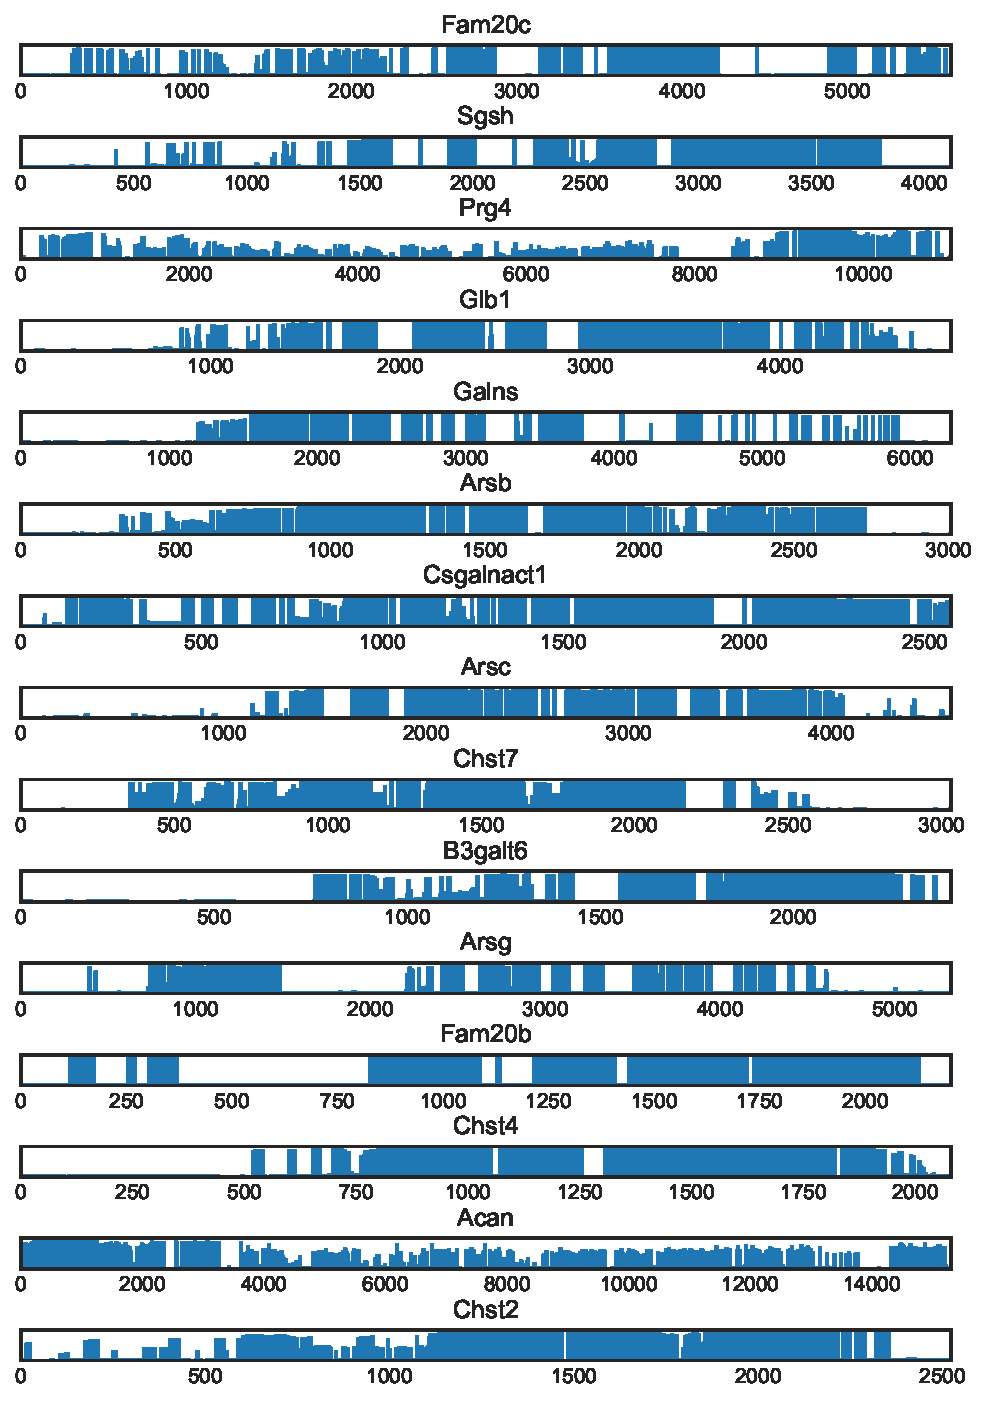
\includegraphics[height=5.5in]{./images/sample_msa.pdf}
\caption{\textbf{A subset of a representation of the gene MSAs.} The \textit{x} axis represents the length of the alignment (number of nucleotides) whereas the \textit{y} axis represents the column similarity, which is the ratio between the number of non-gap characters in a sequence alignment column and the total number of characters in the column. The column similarity is calculated from the MSA of all the organisms whose genomes contain the gene that an MSA represents.}
\label{fig_1}
\end{figure*}

\subsubsection{Core proteins}
The two core genes that were evaluated are \textit{Acan} and \textit{Prg4}. The MSA of \textit{Acan} contains regions that were successfully aligned across the entire length of the gene. Multiple column similarities values that are not higher than 50\% are present throughout the alignment. The MSA of \textit{Prg4} showcases similarities with the MSA of \textit{Acan} but contains a higher proportion of regions of column similarities that are less than 50\%.

\subsubsection{Xylosyltransferases}
The two xylosyltransferase genes that were evaluated are \textit{Xylt1} and \textit{Xylt2}. The MSA of \textit{Xylt1} and \textit{Xylt2} showcase similar patterns. Both MSAs showcase regions that exhibit high conservation based on column similarity indices but have flanking regions with low similarity/a large number of alignment gaps.

\subsubsection{Galactosyltransferases}
The evaluated galactosyltransferase genes are \textit{B3galt6, B4galt7, Chsy1, Chsy3, Csgalnact1,} and \textit{Csgalnact2}. The MSA of \textit{B3galt6} showcases two regions of high conservation between nucleotide 1500 and the end of the sequence. The MSA of \textit{B4galt7} exhibits four regions of high conservation, which are separated by shorter regions of several hundreds of nucleotides. The MSA of \textit{Chsy1} showcases high conservation based on the number of regions that are conserved and the consistently high ratio of column similarity. In addition, the region spanning the first 600 nucleotides showcases low column similarity. The MSA of \textit{Chsy3} showcases similar conservation patterns to \textit{Chsy1} as both genes have a starting region spanning several hundreds of nucleotides with low column similarity but exhibit wide regions of conservation. The alignments of \textit{Csgalnact1} and \textit{Csgalnact2} exhibit wide regions of similarity. However, \textit{Csgalnact2} contains a region of low similarity from position 0 to position 100 of the alignment. In addition, \textit{Csgalnact2} contains 3 regions of low similarity within the alignment. 

\subsubsection{Glucuronyltransferases}
The evaluated glucuronyltransferase genes are \textit{B3gat3, Chpf,} and \textit{Chst1}. The alignment of \textit{B3gat3} contains two regions of approximately 400 nucleotides that are conserved across all organisms' genes. In addition, the alignment showcases interspersed short regions that are conserved - approximately 50-100 nucleotides - with varying column similarities. The MSA of \textit{Chpf} showcases conserved regions across the lengths of the aligned genes. However, the first 250 nucleotides were either not aligned and resulted in multiple gaps or were aligned but resulted in low similarity scores. Lastly, the alignment of \textit{Chst1} showcases a conserved region of approximately 750 nucleotides with the rest of the alignment containing short regions of approximately 50 nucleotides that were aligned.

\subsubsection{Glycosyltransferases}
The evaluated glycosyltransferase genes are \textit{Ext1} and \textit{Ext2}. The MSA of \textit{Ext1} showcases conservation across the gene with the exception of a short region of approximately 400 nucleotides at the beginning of the alignment. The alignment of \textit{Ext2} exhibits conservation across the second half of the gene with the first half of approximately 2000 nucleotides showcasing low or not conservation - low column similarity score or gaps across the entire column.

\subsubsection{Sulfotransferases}
The evaluated sulfotransferase genes are \textit{Chst1, Chst11, Chst12, Chst13, Chst14, Chst15, Chst2, Chst3, Chst4, Chst7, Chst9,} and \textit{Ust}. The alignment of \textit{Chst1} presents a conserved region from nucleotide 2200 to 3100 with the rest of the alignment showcasing either low column similarity or no conservation. \textit{Chst11} exhibits a conserved region from nucleotide 1000 to approximately 1800 with the rest of the alignment containing short regions of high similarity interspersed between regions of low or non-existing column similarity. The alignment of \textit{Chst12} showcases conservation from location 1600 to the end of the gene sequence with multiple short regions of several hundreds of nucleotides that are conserved. \textit{Chst13}'s alignment contains a conserved region from nucleotide 1600 towards the end of the gene alignment. The first half of the alignment showcases 6 short regions that exhibit conservation with the rest being either low conservation or no conservation. The alignment of \textit{Chst14} showcases a conserved region of approximately 750 nucleotides towards the end of the alignment with the first half containing either non-existing or low conservation patterns. The MSA of \textit{Chst15} showcases long conserved regions of approximately 1500 and 500 nucleotides, respectively, separated by a short region of low column similarity of approximately 100 nucleotides. In addition, the beginning of the alignment contains a region of approximately 300 nucleotides that showcase low column similarity. The alignment of \textit{Chst2} showcases a continuous region of high similarity between nucleotides 1000 and approximately 2600. The alignment region before nucleotide 1000 showcases column similarity values between 50 and approximately 80\%. The alignment of \textit{Chst3} showcases a conserved region from nucleotide 1000 to approximately 2400 with the region between nucleotide 500 and 1000 showcasing high and low column similarity ranging from approximately 10 to 80\%. The alignment of \textit{Chst4} showcases 3 highly conserved regions between nucleotide 750 and 1000, 1100 and 1250, and 1300 and 2000, respectively. The first 500 nucleotides in the alignment showcase low to no column similarity. The alignment of \textit{Chst7} showcases regions of similarity clustered towards the middle of the alignment from nucleotide 400 to 2200. The conserved regions contain column similarity values ranging from approximately 10 to 100\%. Lastly, the alignment of \textit{Chst9} showcases a conserved region from nucleotide 800 to 1750 and from nucleotide 1800 to 2200. The first 800 nucleotides contain short conserved regions with length ranging from 20 to 100 nucleotides. 

\subsubsection{Sulfatases}
The evaluated sulfatase genes are \textit{Arsa, Arsb, Arsc, Arsd, Arse, Arsf, Arsg, Arsi, Arsj, Arsk, Galns, Gns, Ids, Sulf1, Sumf1,} and \textit{Sumf2}. The alignment of \textit{Arsa} showcases multiple short conserved regions ranging in length from approximately 50 nucleotides  to 400 nucleotides. The beginning of the alignment contains a region of 500 nucleotides that showcase low conservation while the end of the alignment showcases a region of approximately 300 nucleotides with low conservation. The MSA of \textit{Arsb} showcases long conserved regions from nucleotide 500 to approximately 2700 with the first 400 and the last 300 nucleotide regions showcasing low similarity. The MSA of \textit{Arsc} showcases interspersed regions of high similarity between nucleotide 1100 and 4000 with the start and end regions of the alignment showcasing low similarity ranging from approximately 10 to 40\%. The alignment of \textit{Arsd} exhibits a conserved region from nucleotide 1500 towards the end of the sequence. The first 1500 nucleotides showcase low similarity ranging from approximately 10 to 80\%. The alignment of \textit{Arse} showcases conserved regions ranging from approximately 10 to 100\% across a region from nucleotide 500 to 5200 with the flanking regions of the alignment showcasing no similarity. The alignment of \textit{Arsf} showcases similar patterns to the alignment of \textit{Arse} with conserved regions from nucleotide 500 to 4500 and flanking regions of low similarity. The alignment of \textit{Arsg} showcases multiple conserved regions. The conserved regions range from nucleotide 500 to 1500 and 2200 to 4500 with interspersed regions of low similarity. The alignment of \textit{Arsi} showcases 9 regions of high similarity separated by a region of no similarity from nucleotide 2500 to approximately 3800. The MSA of \textit{Arsj} showcases high similarity spread throughout the alignment with short regions of low similarity of lengths ranging from 10 to 50 nucleotides. The alignment of \textit{Arsk} showcases multiple regions of high similarity ranging from nucleotide 1500 to 3300 with multiple short regions of lengths ranging from 20 to 50 nucleotides surrounding the regions of high similarity. The flanking regions of the alignment represent conservation regions of 500 nucleotides. The MSA of \textit{Galns} showcases a conserved region from nucleotide 1000 to approximately 3000, which are separated by approximately 8 regions of low similarity of length 10 to 50 nucleotides. The rest of the alignment showcases multiple short regions of 10 to 40 nucleotides that showcase high similarity across the alignment. The MSA of \textit{Gns} showcases a conserved gene region from nucleotide 1700 to 3500. The first half of the alignment contains a highly conserved region from nucleotide 1000 to 1400 with the rest of the alignment showcasing low to no similarity. The MSA of \textit{Ids} showcases multiple regions that are highly conserved across the gene with lengths ranging from 50 to 200 nucleotides. The first 1800 nucleotides of the alignment showcase column similarity values ranging from approximately 10 to 50\%. The alignment of \textit{Sulf1} showcases 3 highly conserved regions of approximately 500 nucleotides with multiple, short, highly conserved regions spread throughout the alignment. The region from nucleotide 5000 to 7000 contains similarity values ranging from 40 to approximately 80\%. The MSA of \textit{Sumf1} contains two regions of high similarity from nucleotide 1500 to 2000 and 2200 to 2400, respectively. The region from nucleotide 500 to 1500 showcases similarity values ranging from 20 to 80\% with the flanking regions of the alignment showcasing low column similarity values of approximately 10\%. Lastly, the MSA of \textit{Sumf2} showcases conserved regions ranging from the start of the gene alignment to nucleotide 2000. The second half of the alignment contains either low similarity or no similarities. 

\subsubsection{Kinases}
The evaluated kinase genes are \textit{Fam20a, Fam20b,} and \textit{Fam20c}. The MSA of \textit{Fam20a} contains a highly conserved region from nucleotide 4000 to the end of the alignment. The first 4000 nucleotides contain interspersed regions of short length - approximately 50 nucleotides - but high column similarity values - approximately 80\%. The alignment of \textit{Fam20b} showcases 9 distinct nucleotide regions that are highly conserved with regions of low conservation scattered between. The longest region of low similarity ranges from nucleotide 400 to approximately 800. The alignment of \textit{Fam20c} showcases three regions of high similarity with length ranging from 200 to 400 nucleotides. The rest of the alignment contains short regions of 20 to 100 nucleotides that are highly conserved.

\subsubsection{Epimerases}
The evaluated epimerase gene is \textit{Dse}. The MSA of \textit{Dse} showcases a highly conserved region of approximately 3000 nucleotides. In addition, the alignment showcases multiple short regions ranging from 50 to 200 nucleotides that are highly conserved. The first 600 nucleotides showcase low similarity across the alignment. 

\subsubsection{Glycosidases}
The evaluated glycosides gene is \textit{Gusb}. The alignment of \textit{Gusb} contains several highly conserved regions. Specifically, the alignment showcases 4 regions of lengths ranging from 200 to 600 nucleotides that are highly conserved. In addition, the alignment showcases multiple short regions of length ranging from 20 to 100 nucleotides that are highly conserved.

\subsubsection{Sulfohydrolases}
The evaluated sulfohydrolase gene is \textit{Sgsh}. The MSA of \textit{Sgsh} contains a region that is highly conserved between nucleotide 2800 to 3700. In addition, the alignment showcases 4 regions that are approximately 200 nucleotides in length and showcase high similarity. The rest of the alignment contains scattered regions of low column similarity. 

\subsection{Taxonomic information}
The collection of taxonomic information resulted in a record being produced for every organism used in this study. Organisms were grouped by taxonomic class. Figure \ref{fig_2} provides a summary of the number of organisms in each taxonomic category that was used for categorizing organisms. Significant organisms were selected from each taxonomic group outlined in Figure \ref{fig_2}, which resulted in the 21 organisms outlined in Table \ref{tab_2}.

\subsection{Phylogenetic relationships}
The phylogenetic relationships between all the genes used in this study were captured and visualized, which resulted in 51 "gene trees". Figure \ref{fig_3} represents a sample "gene tree" that was constructed from a phylogenetic tree that represents the evolutionary relationship between all the organisms used in this study. Trees were grouped based on organisms' genetic similarity using Algorithm \ref{alg_1}, which resulted in a reduction from 51 trees to 16. Table \ref{tab_1} outlines the "gene trees" that were combined into a single tree.

\begin{figure}[]
\centering
\makebox[\textwidth][c]{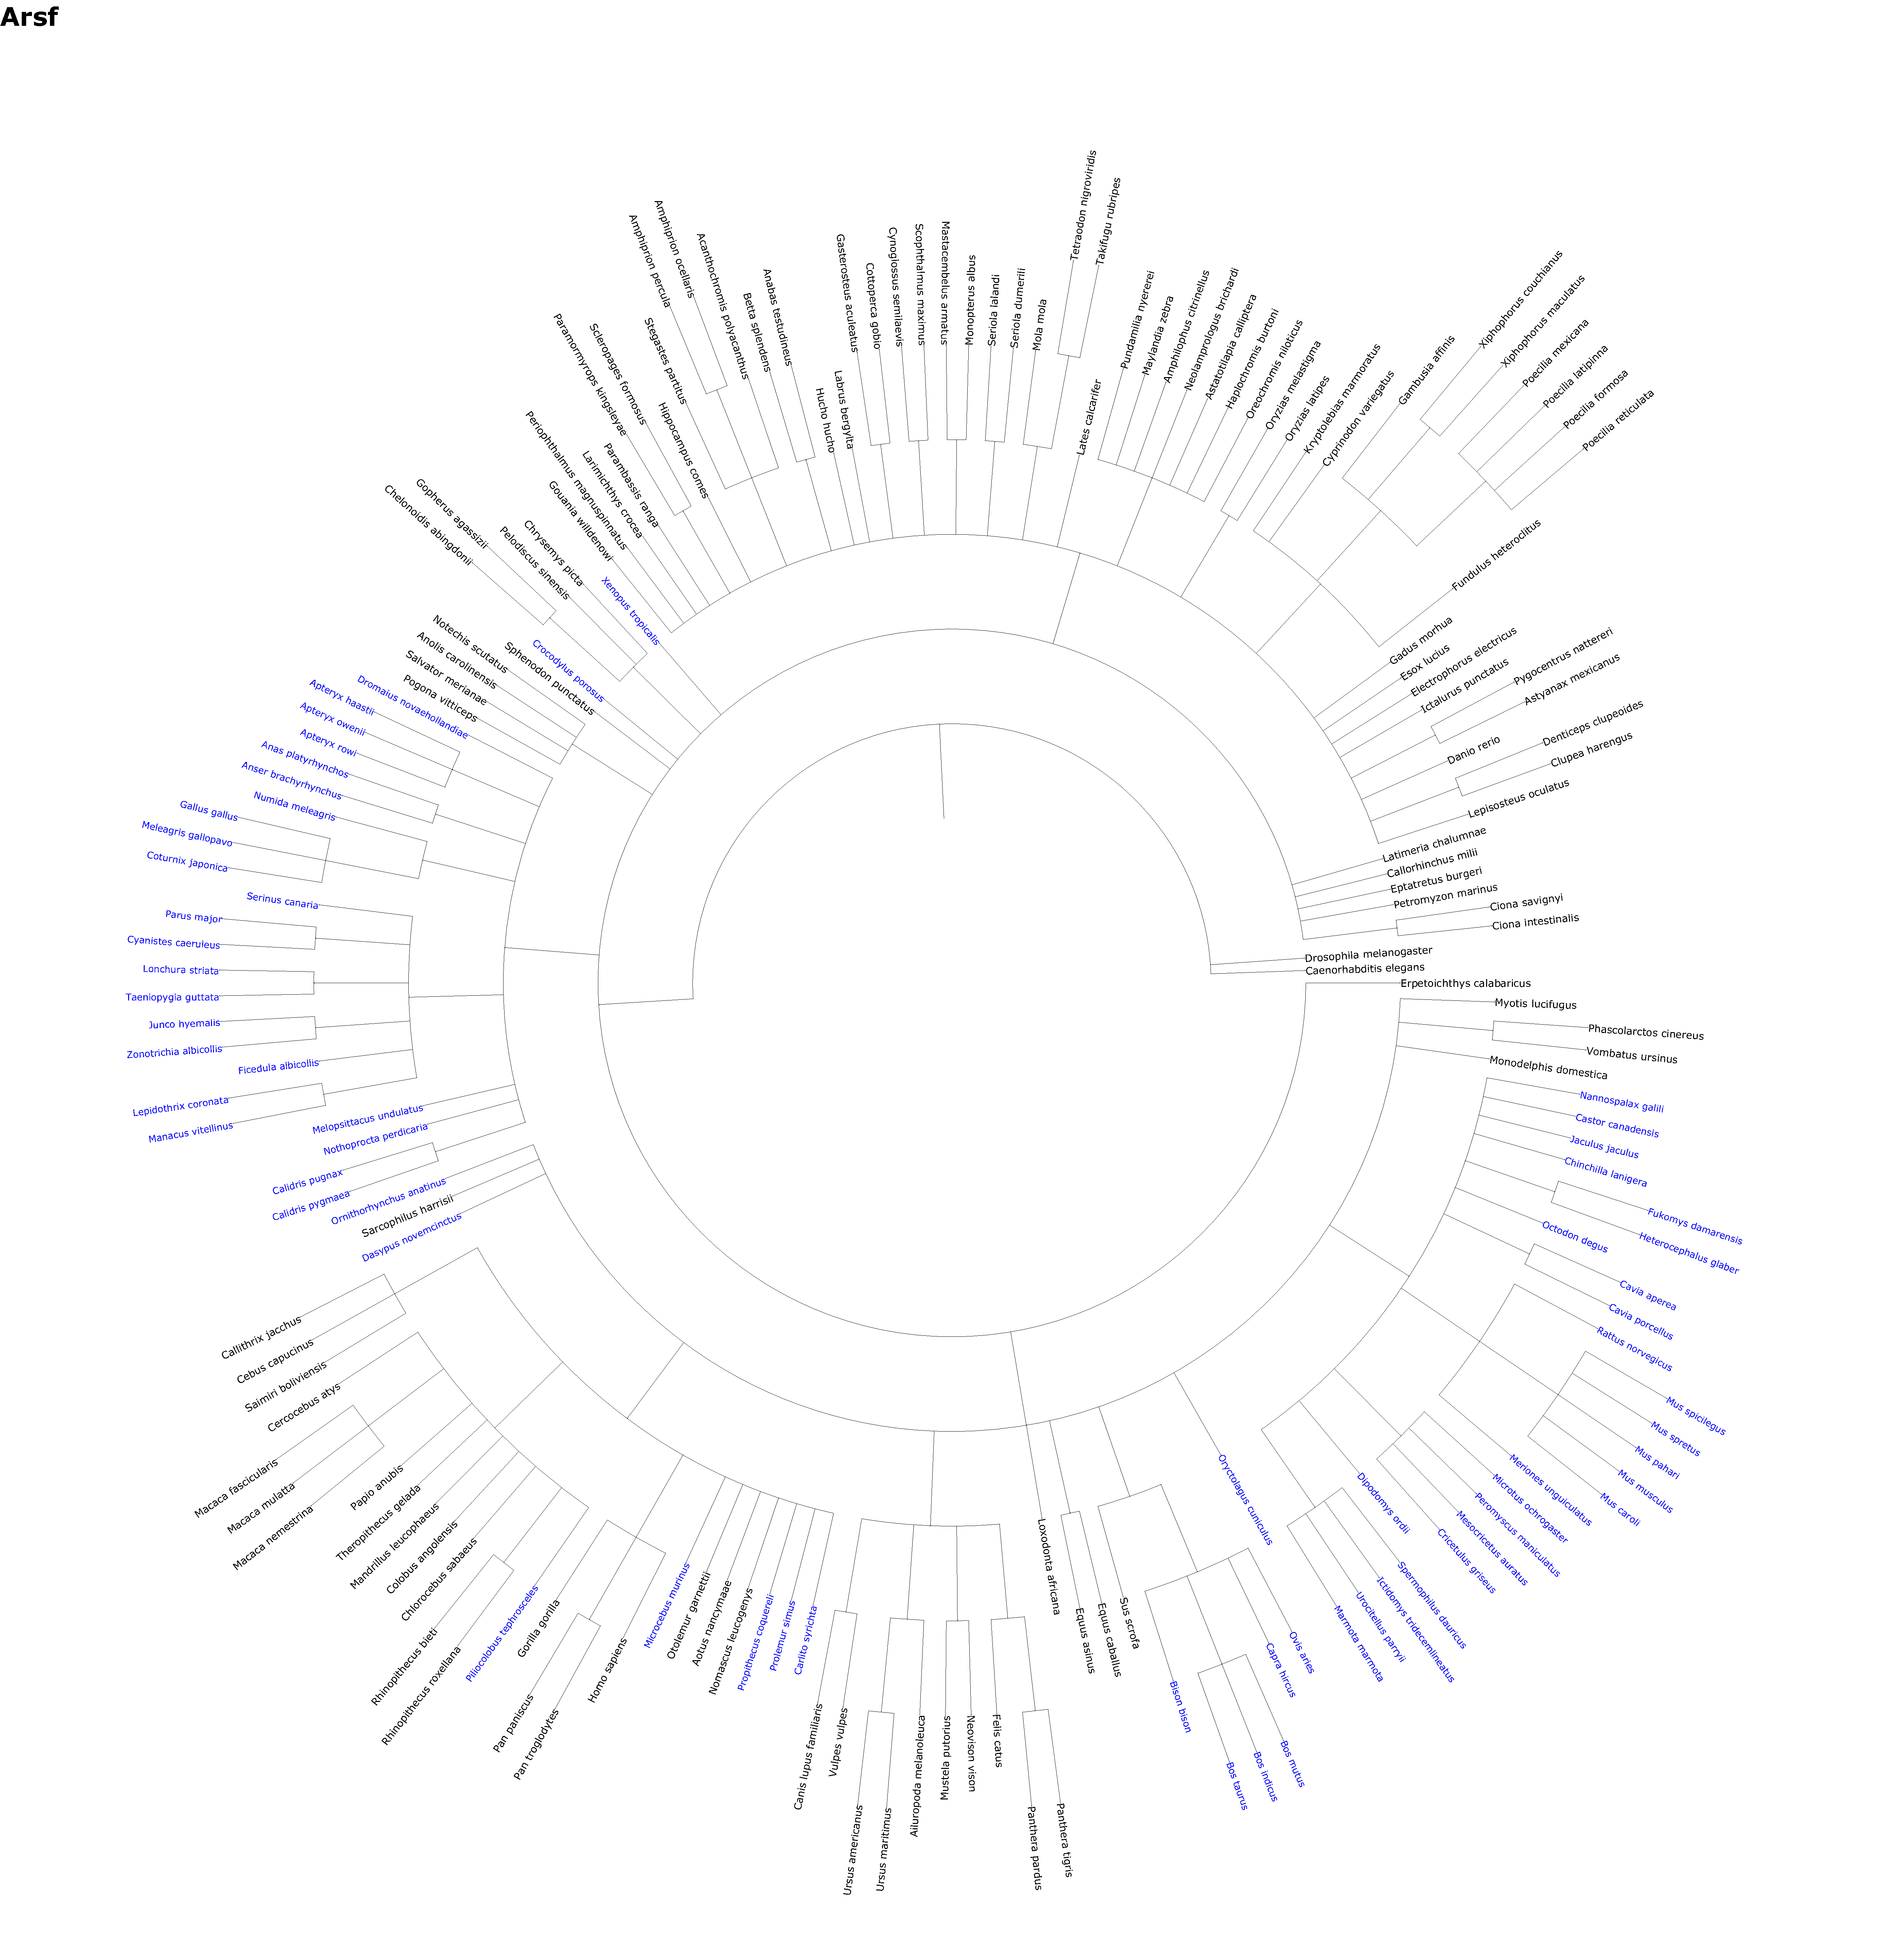
\includegraphics[height=7in,trim={0 0 0 3in},clip]{./images/tree_sample_arsf.pdf}}
\caption{\textbf{The gene tree for \textit{Arsf}.} The blue leaves represent organisms that do not have \textit{Arsf} in their genomes whereas black leaves represent organisms that have \textit{Arsf} in their genomes. The tree was constructed from a global phylogenetic tree representing the relationships between the organisms included in this study.}
\label{fig_3}
\end{figure}

\begin{table}[]
\begin{tabular}{llllll}
\hline
Class             		& Organism                          		& Terrestrial	& Aquatic		& Cartilage                 & Bone	\\ 
\hline
Mammalia        		& \textit{Homo sapiens}             		& \checkmark 	&              		& \checkmark & \checkmark 	\\
                  		& \textit{Mus musculus}             		& \checkmark 	&              		& \checkmark & \checkmark 	\\
                  		& \textit{Ornithorhynchus anatinus} 	& \checkmark 	&			& \checkmark & \checkmark 	\\
Actinopterygii    	& \textit{Danio rerio}              		&                       & \checkmark 	& \checkmark & \checkmark 	\\
                  		& \textit{Oryzias latipes}          		&                       & \checkmark 	& \checkmark &                    	\\
                  		& \textit{Takifugu rubripes}        		&                       & \checkmark 	& \checkmark &                       	\\
                  		& \textit{Lepisosteus oculatus}     	&                       & \checkmark 	& \checkmark &                        	\\
Archelosauria   		& \textit{Anas platyrhynchos}       	& \checkmark 	& \checkmark 	& \checkmark & \checkmark 	\\
                  		& \textit{Gallus gallus}            		& \checkmark 	&                       & \checkmark & \checkmark 	\\
                  		& \textit{Chrysemys picta bellii}   	&                       & \checkmark 	& \checkmark & \checkmark 	\\
                  		& \textit{Crocodylus Porosus}       	& \checkmark 	& \checkmark 	& \checkmark & \checkmark 	\\
Lepidosauria    		& \textit{Notechis scutatus}        	& \checkmark 	&                       & \checkmark & \checkmark 	\\
                  		& \textit{Anolis carolinensis}      		& \checkmark 	&                       & \checkmark & \checkmark 	\\
Amphibia          		& \textit{Xenopus tropicalis}       	& \checkmark 	& \checkmark 	& \checkmark & \checkmark 	\\
Holocephali      		& \textit{Callorhinchus milii}      		&                       & \checkmark 	& \checkmark &                 	\\
Coelacanthiformes 	& \textit{Latimeria chalumnae}      	&                       & \checkmark 	& \checkmark & \checkmark 	\\
Hyperoartia       	& \textit{Petromyzon marinus}       	&                       & \checkmark 	& \checkmark & \checkmark 	\\
Hyperotreti       		& \textit{Eptatretus burgeri}       		&                       & \checkmark 	& \checkmark & \checkmark 	\\
Phlebobranchia    	& \textit{Ciona intestinalis}       		&                       & \checkmark 	&                           &                  	\\
Pterygota         		& \textit{Drosophila melanogaster}  	& \checkmark 	&                       &                           &                 	\\
Rhabditina        		& \textit{Caenorhabditis elegans}   	& \checkmark 	& \checkmark 	&                           &                   \\
\hline       
\end{tabular}
\caption{\textbf{An outline of the subset of organisms chosen as representatives.}}
\label{tab_2}
\end{table}

\begin{table}[]
\begin{tabular}{ll}
\hline
\textbf{Tree} & \textbf{Genes}													\\ 
\hline
1             & \textit{Arsc, Arsi, Dse, Ext1}                                               						\\
2             & \textit{Arsd, Arsj}                                                          						\\
3             & \textit{Arse}                                                                							\\
4             & \textit{Arsf}                                                                							\\
5             & \textit{B3galt6, Chst13}                                                     						\\
6             & \textit{Chst3, Xylt2, Gns, Acan, Chst1}                                      					\\
7             & \textit{Chst4}                                                               						\\
8             & \textit{Chst7, B4galt7, Fam20b}                                              					\\
9             & \textit{Chst9}                                                               						\\
10            & \textit{Chst12, Chst15, Glb1, Arsg, Fam20a, Chst2, Chpf, Gusb, Chsy1, Sumf1} 	\\
11            & \textit{Chst14}                                                              						\\
12            & \textit{Chsy3}                                                               						\\
13            & \textit{Sulf2, Chst11, Csgalnact2, Arsb, Galns, Fam20c, Prg4}                			\\
14            & \textit{Sumf2}                                                               						\\
15            & \textit{Ust, Chpf2, Ext2, Arsa, Sulf1, Arsk, Xylt1}                          				\\ 
\hline
\end{tabular}
\caption{\textbf{An outline of the gene trees that were combined based on organisms' similarity.}}
\label{tab_1}
\end{table}


\begin{figure}[]
\centering
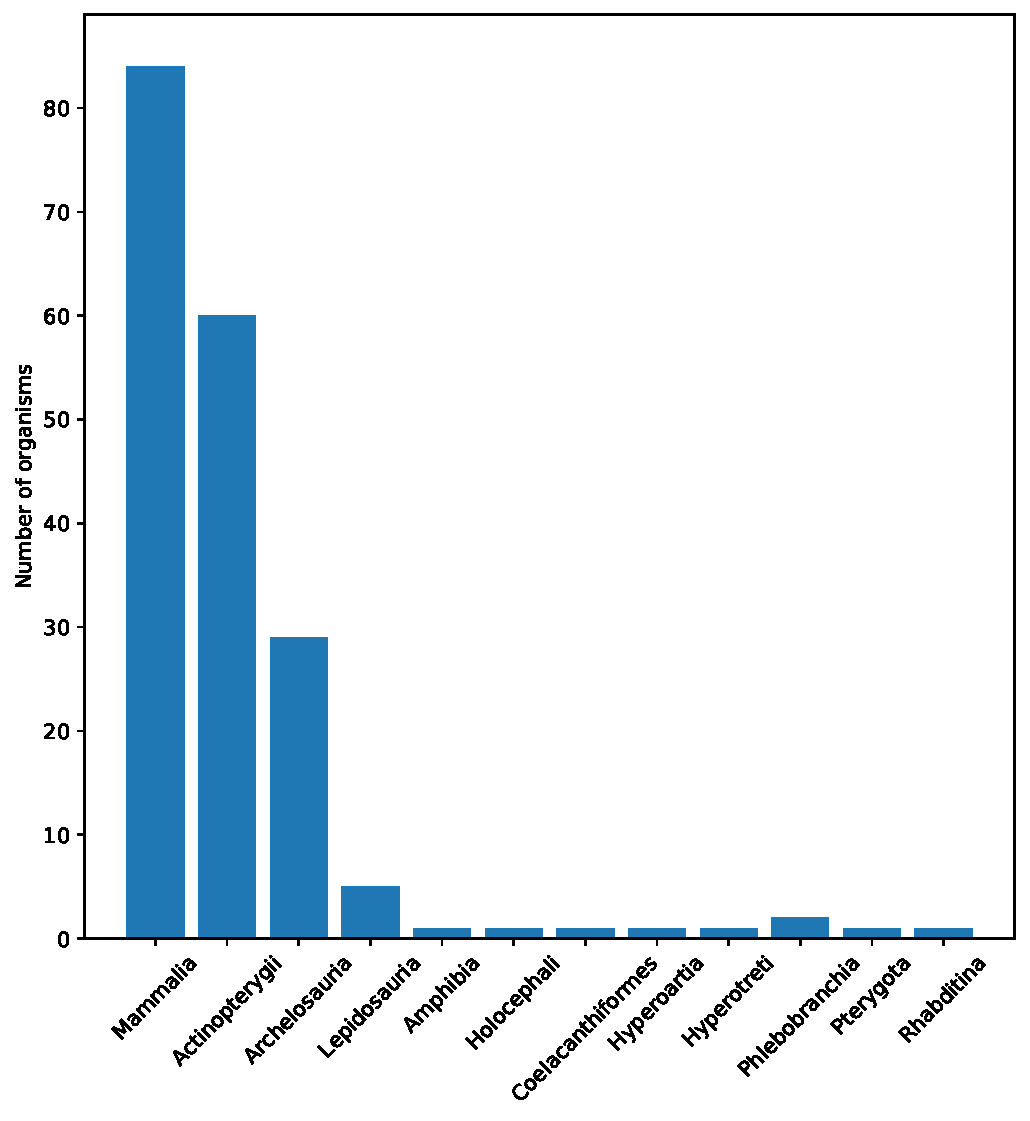
\includegraphics[height=4in]{./images/taxa_info.pdf}
\caption{\textbf{Taxonomic frequency of the analyzed organisms.} The presented classes are: Mammalia - mammals; Actinopterygii - ray-finned fish; Archelosauria - turtles and archosaurs; Lepidosauria - scaly reptiles; Amphibia - amphibians; Holocephali - cartilaginous fish; Coelacanthiformes - bony fish (ancient); Hyperoartia - jawless bony fish; Hyperotreti - hagfish; Phlebobranchia - sea squirts; Pterygota - winged insects; Rhabditina - nematodes.}
\label{fig_2}
\end{figure}

\subsection{dN/dS ratios}

The dN/dS ratios were computed for the chosen significant organisms, which lead to the creation of 21 dN/dS plots. A sample plot is outlined in Figure \ref{fig_4} with the rest of the dN/dS plots available as supplementary information. The results of all 21 dN/dS plots were summarized in Figure \ref{fig_5}. 

The dN/dS summaries of \textit{Homo sapiens, Mus musculus, Ornithorhynchus anatinus, Danio rerio, Oryzias latipes, Takifugu rubripes, Lepisosteus oculatus, Anas platyrhynchos, Gallus gallus, Chrysemys picta, Crocodylus porosus, Notechis scutatus, Anolis carolinensis, Xenopus tropicalis, Callorhinchus millii}, and \textit{Latimeria chalumnae} showcase bimodal distributions with an average of 48\% of the dN/dS values being less than 1 while 52\% of the values are greater than or equal to 1. The dN/dS summaries of \textit{Petromyzon marinus, Eptatretus burgeri, Ciona intestinalis, Drosophila melanogaster}, and \textit{Caernohabditis elegans} showcase the values are approximately normally distributed with a high proportion of the values clustered at the mean and a small variance. Approximately 23\% of the dN/dS values are less than 1. 

The genes dN/dS distributions illustrated by the classification of organisms based on bone, cartilage, or absence of bone and cartilage do not showcase clear statistically significant general differences between the distributions of the genes. The median of the dN/dS distribution for \textit{Fam20b} in organisms without bone or cartilage is approximately 1, compared to the distributions of organisms with bone and organisms with cartilage only that showcase a median of approximately 0.1. By comparison to organisms with bone and organisms without bone and cartilage, the distribution of \textit{Chst4} in cartilaginous organisms is clustered at 1. The dN/dS distribution of \textit{Acan, Chst15, Ext1, Chst13, Chst12, Chst11, Chst1}, and \textit{Chst9} are all clustered at 1 compared to the corresponding distributions in bony organisms and cartilaginous organisms. 

The genes dN/dS distributions illustrated by the classification of organisms based on terrestrial, aquatic, or both terrestrial and aquatic habitats do not showcase clear statistically significant inter-group differences. The distribution of \textit{Sumf2} in organisms that live in terrestrial and aquatic environments is clustered at 1 compared to the distribution of the same gene in organisms that are terrestrial and organisms that are aquatic. 

\begin{figure}[]
\centering
\makebox[\textwidth][c]{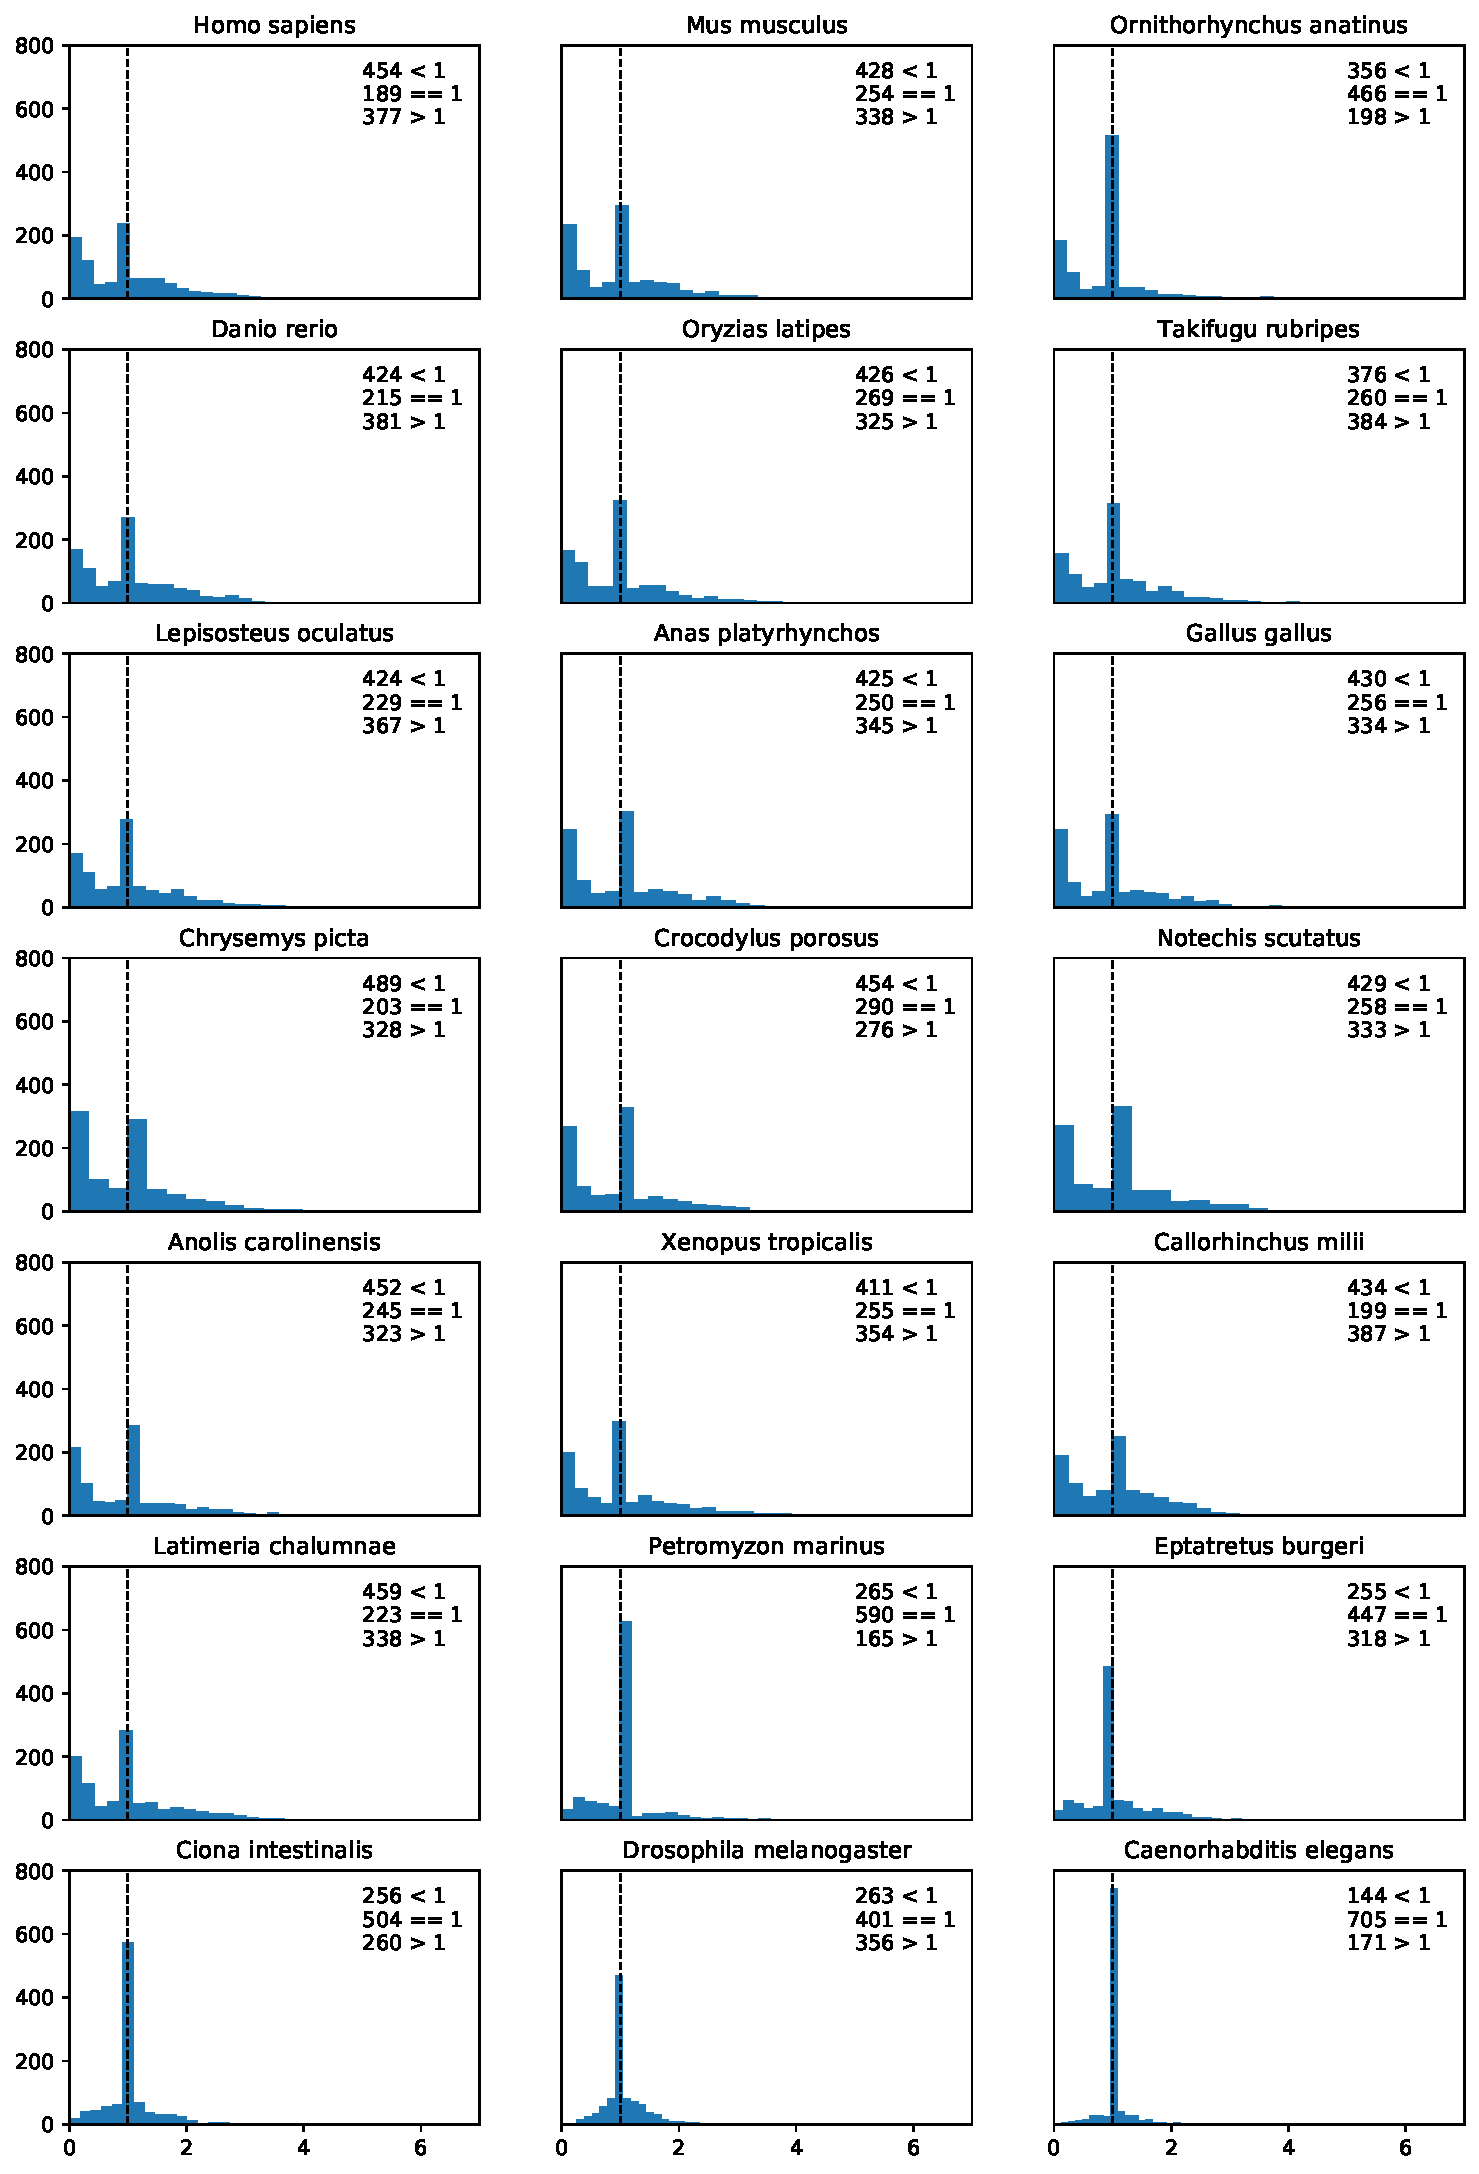
\includegraphics[height=7in,trim={0 0 0 0in},clip]{./images/dnds_histo.pdf}}
\caption{\textbf{Histograms representing the distribution of dN/dS values for each significant organism.} The histograms include a marker at the value of 1 to represent neutrality. The number of dN/dS values less than and greater than or equal to 1 are indicated.}
\label{fig_5}
\end{figure}

\begin{figure}[]
\centering
\makebox[\textwidth][c]{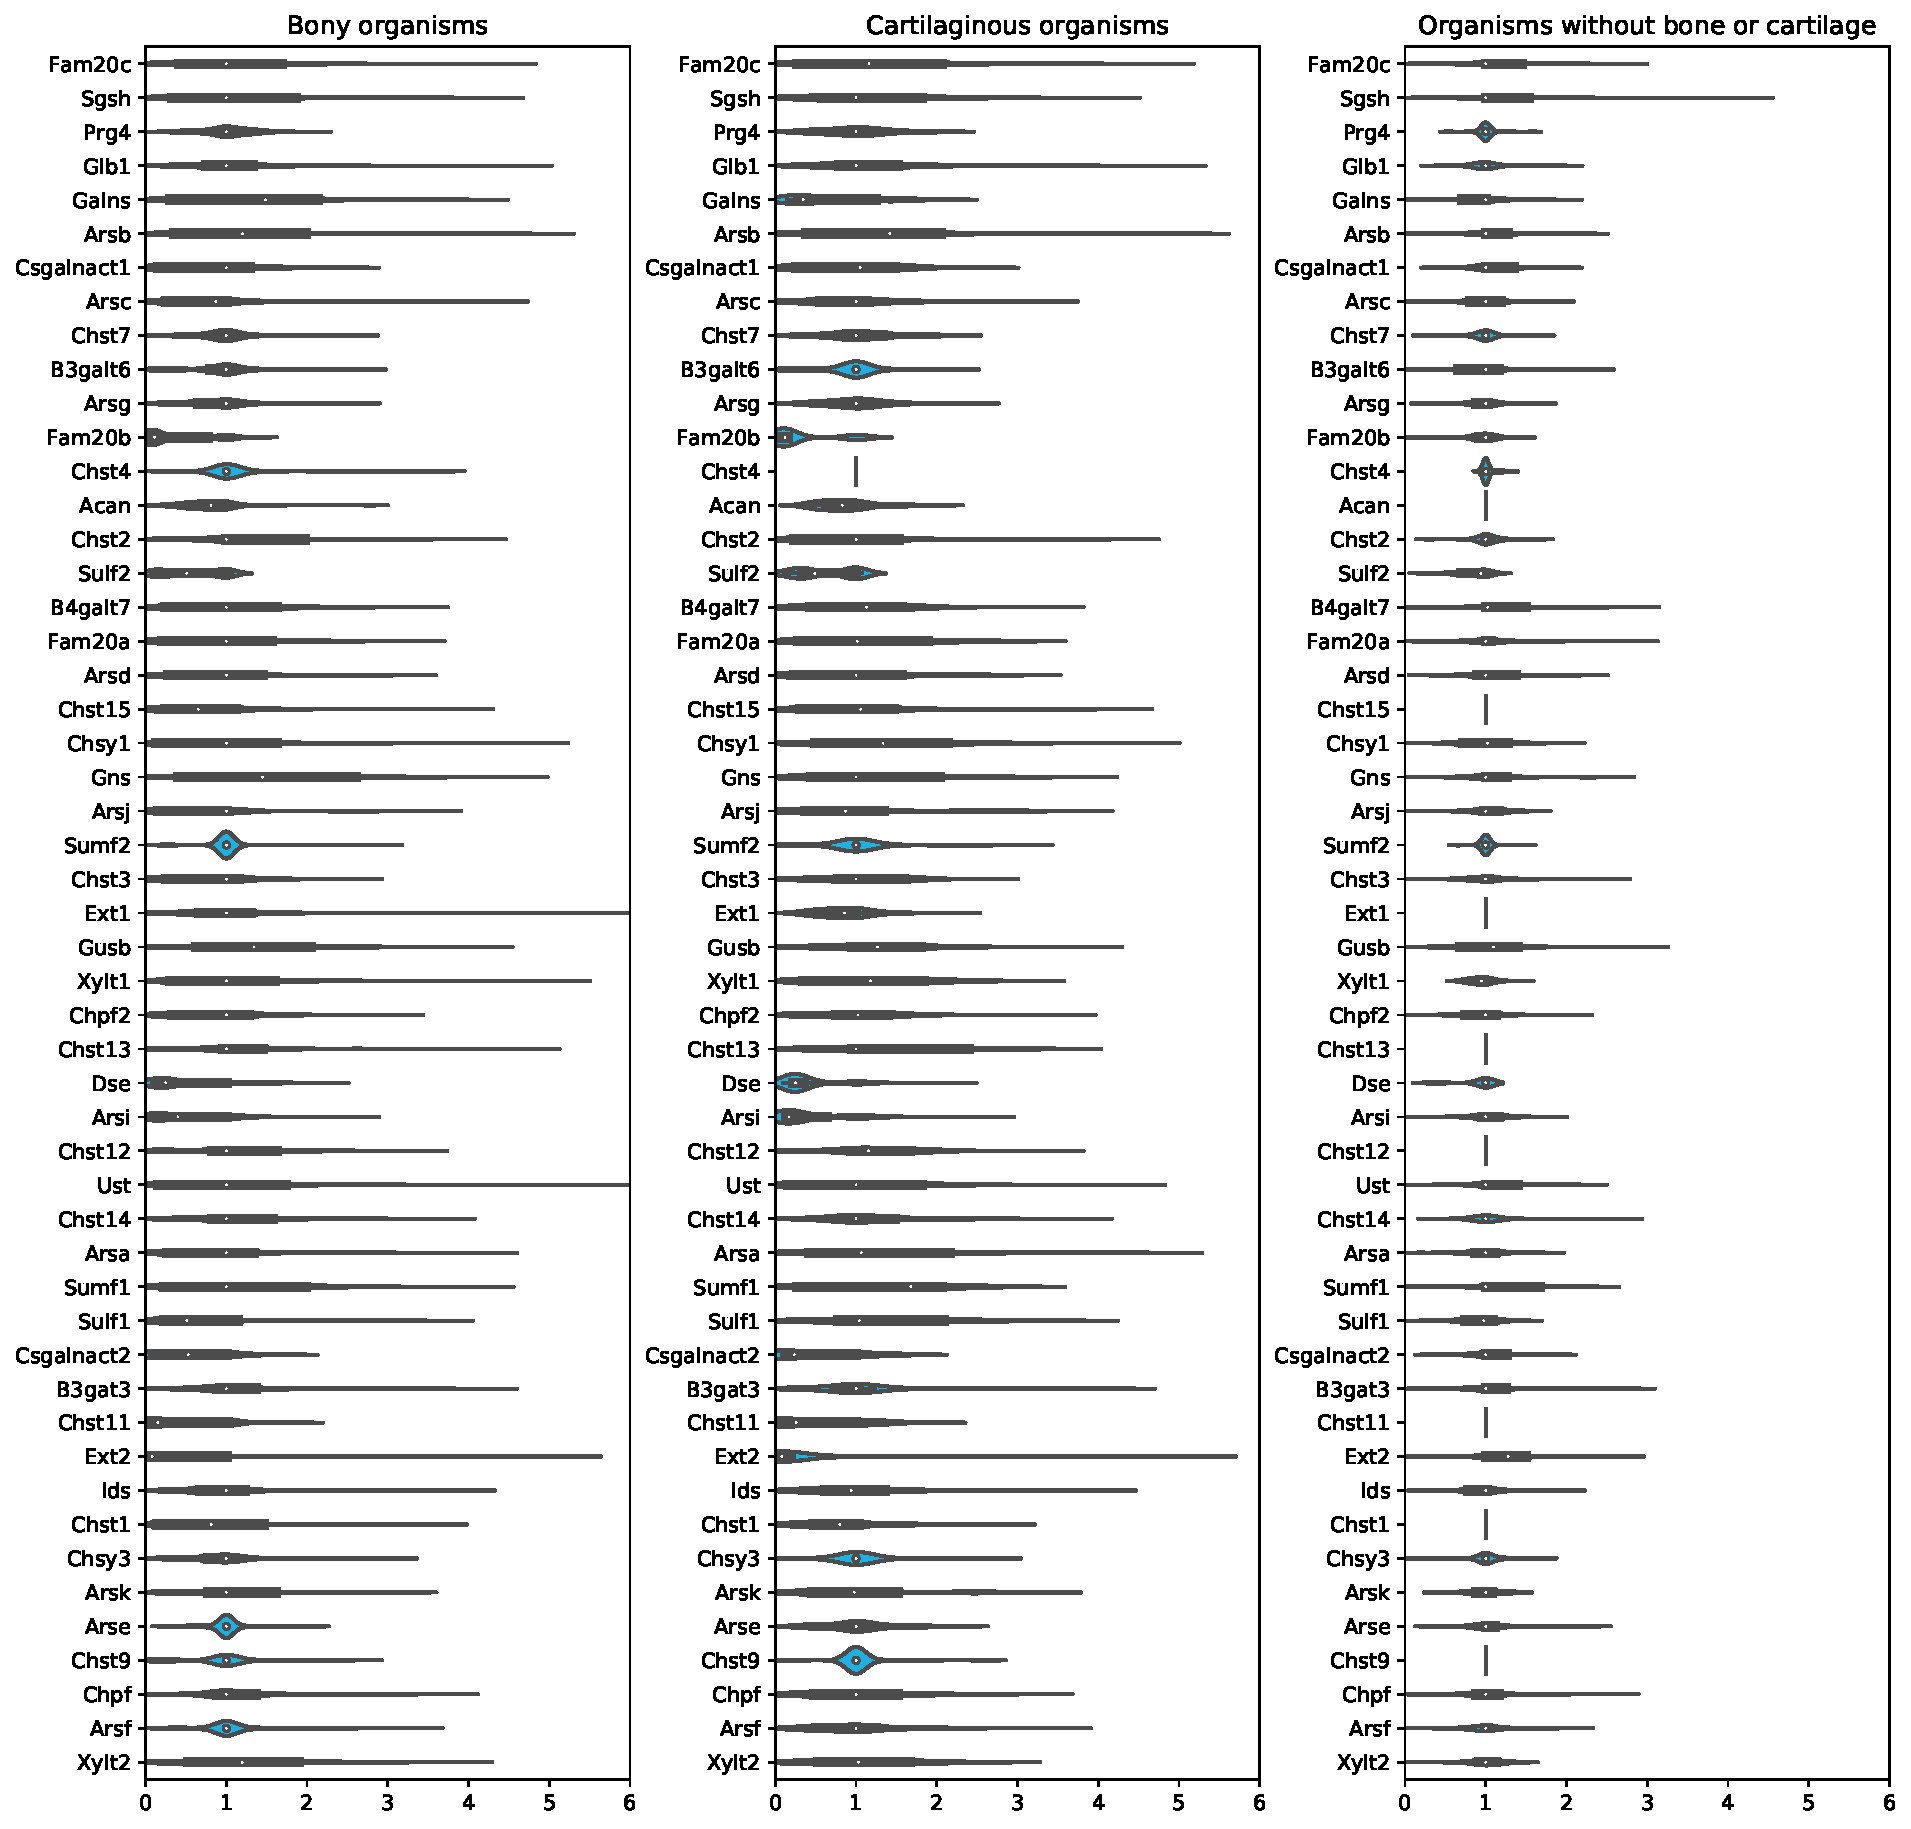
\includegraphics[height=7in,trim={0 0 0 0in},clip]{./images/bone_dist.pdf}}
\caption{\textbf{Violin plots for the dN/dS values of each independent gene binned by organism bone or cartilage presence presence.}}
\label{fig_6}
\end{figure}

\begin{figure}[]
\centering
\makebox[\textwidth][c]{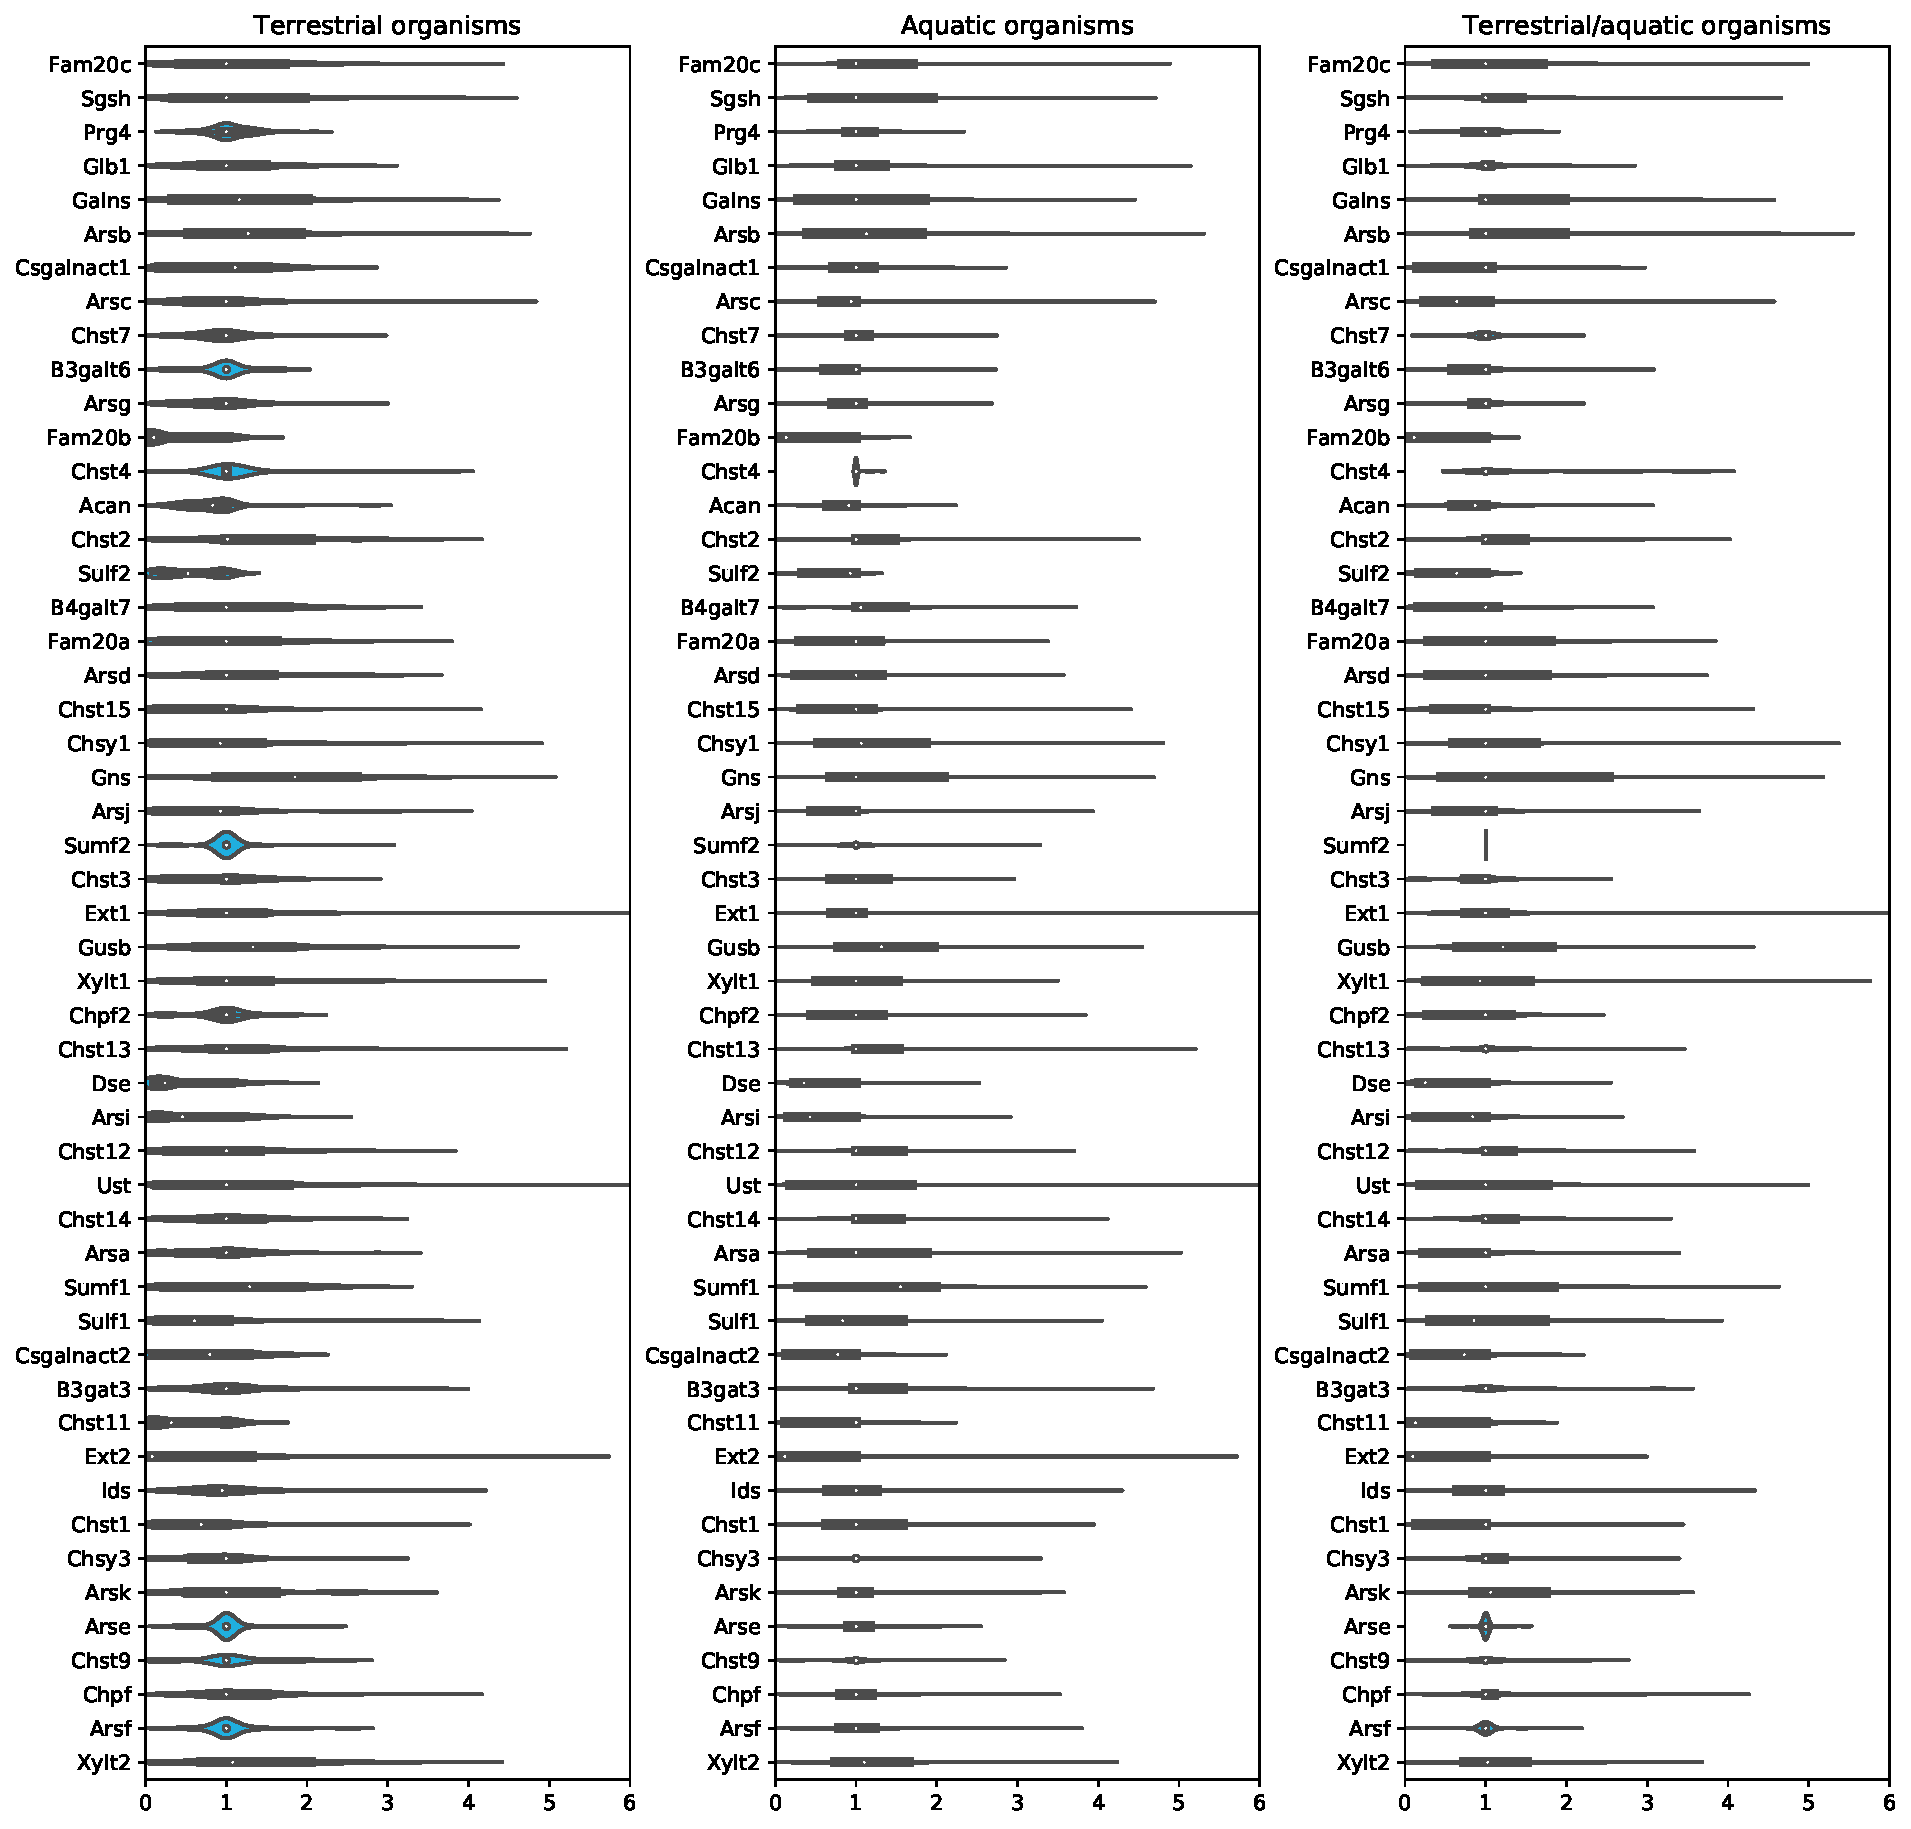
\includegraphics[height=7in,trim={0 0 0 0in},clip]{./images/habitat_dist.pdf}}
\caption{\textbf{Violin plots for the dN/dS values of each independent gene binned by organism habitat.}}
\label{fig_7}
\end{figure}

\begin{figure}[]
\centering
\makebox[\textwidth][c]{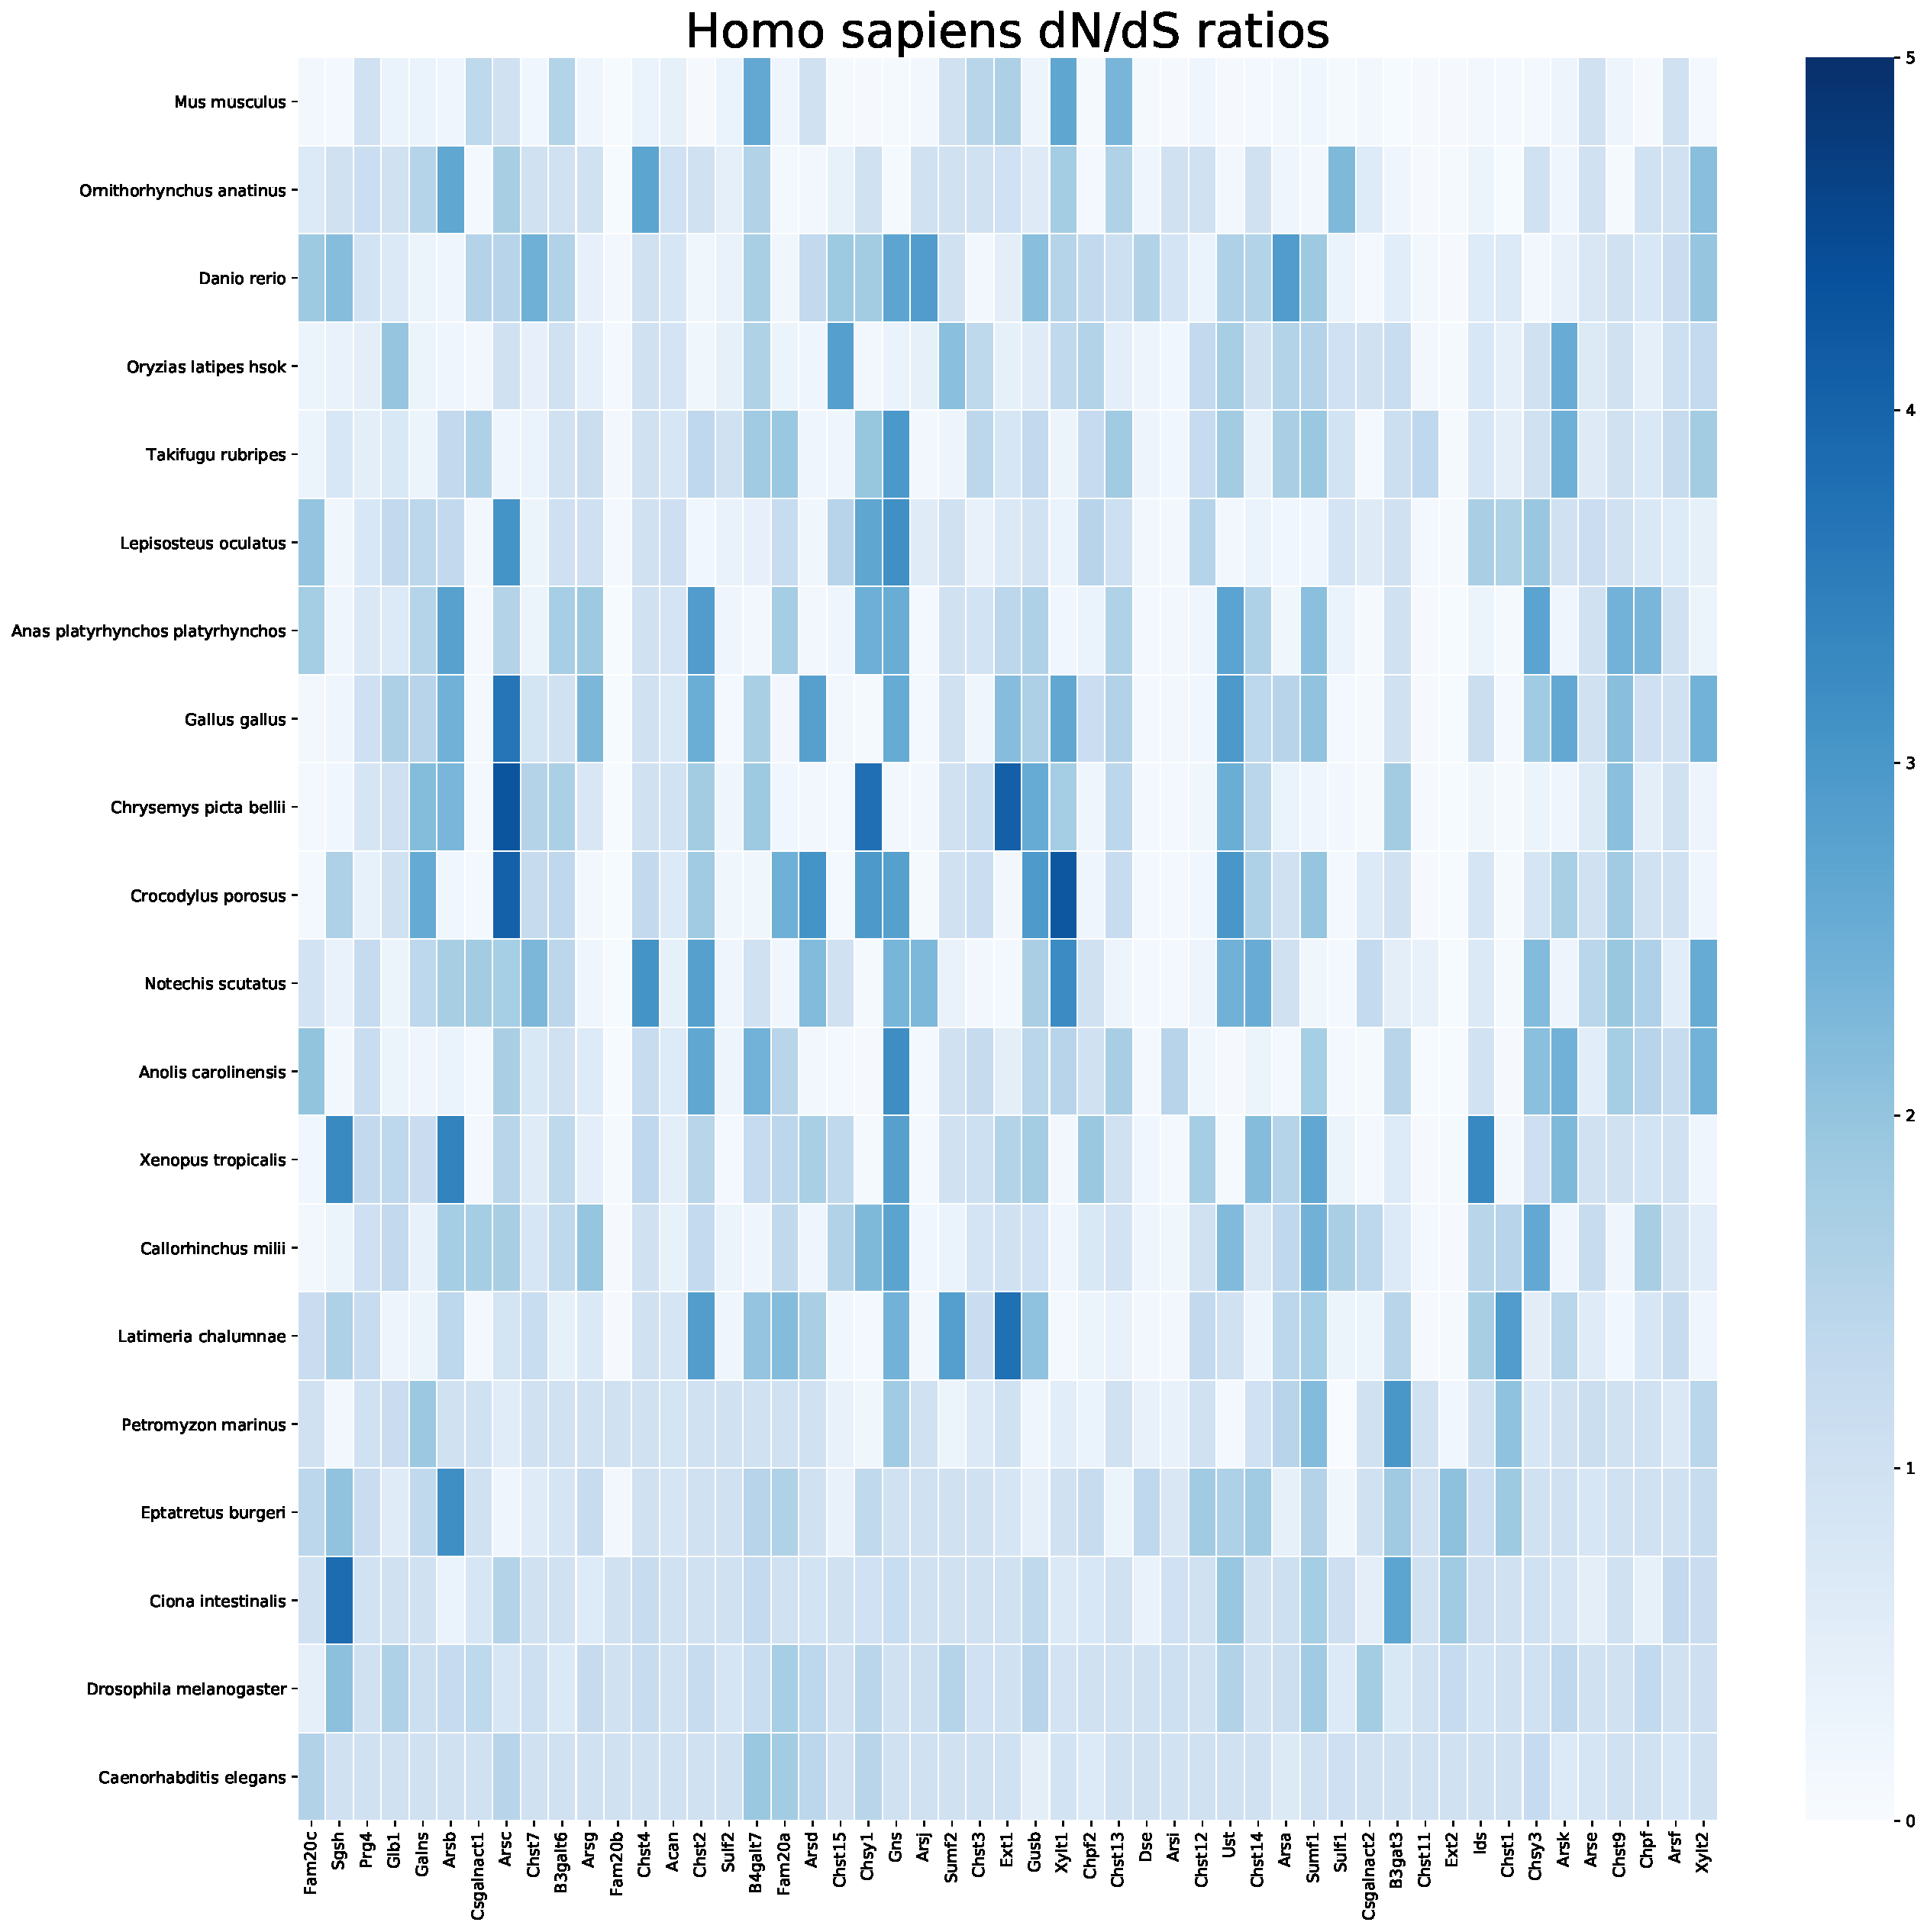
\includegraphics[height=7in,trim={0 0 0 0in},clip]{./images/homo_sapiens_dnds.pdf}}
\caption{\textbf{A sample dN/dS 2D grid for \textit{Homo sapiens} computed against the other significant organisms.} The intensity values represent the dN/dS ratio - values lighter in colour are less than 1 and purifying selection while values darker in colour are greater than 1 and represent positive selection.}
\label{fig_4}
\end{figure}

\section{Discussion}
In this research, the sequence conservation, phylogenetic relationships, and mutation rates of genes of the proteoglycan synthesis pathway were inspected. The study was initiated by first collecting all the proteogylcan synthesis pathway gene orthologs of \textit{Homo sapiens} from Ensembl. \textit{Homo sapiens} was chosen as the model organism as it contains all the 51 genes that are involved in the synthesis of proteoglycan. Ensembl was chosen as the source database as the genomes of the organisms present in Ensembl are annotated and curated. Of the 199 collected organisms, only 187 were used. The 12 organisms that were excluded were projection builds, which were removed due to the uncertainty associated with the correctness of gene presence. For example, \textit{Vicugna pacos}' genome is reported to not contain \textit{Acan}, which is a core protein-coding gene involved in synthesizing proteoglycan. Errors such as the previously mentioned example may serve to motivate additional effort expenditure in the area of genome annotation, which is critical for performing inferences and testing hypotheses. 

Collected gene sequences were aligned, which resulted in 51 MSAs. The alignment results were enumerated by grouping genes according to their function as it was expected for genes with similar function to showcase intergroup alignment similarities. The group of core proteins showcase alignments that contain conserved regions across their entirety. Conservation in the alignments of core proteins suggests that the sequences of these core proteins is generally undergoing negative selection (conservation). This is an expected outcome since it is accepted that \textit{Acan} is an important protein-coding gene involved in binding water molecules within cartilage \cite{proteo_osteo1}, suggesting it's sequence should be highly conserved across organisms. Xylosyltransferase showcased similar conservation patterns within the alignment but contained flanking regions that were less conserved. It is possible that sections of the sequence of \textit{Xylt1} and \textit{Xylt2} are critical for normal proteoglycan function, since xylosyltransferases catalyze the carbohydrate chain addition to core proteoglycan proteins \cite{xylt}. Galactosyltransferase genes showcased several differences between sequence conservation patterns, which is inconsistent with previous findings that illustrate the importance of their conservation. Significant parts of alignments have not been identified to have high column similarity, as exemplified by the alignment of \textit{B3galt6}. While it has been previously suggested that sequence conservation in galactosyltransferase genes is important, it may be manifested independently within genes rather than between them. Since the group of galactosyltransferases contains 6 genes (\ref{sup_fig_2}), it is possible for gene redundancy to manifest as some genes may have higher transcription rates compared to others \cite{galt}. Glucuronyltransferases showcased similar sequence alignment patterns to galactosyltransferases but exhibited more sparsity, which suggests this group of genes may undergo higher mutation rates compared to galactosyltransferases. \textit{Ext1} and \textit{Ext2}, which are glycosyltransferase protein-coding genes, showcased unexpected alignments as \textit{Ext1} exhibited highly conserved nucleotide regions across the entire alignment by comparison to \textit{Ext2}, which showcased almost no conservation across the first 2000 nucleotides. Since \textit{Ext1} binds \textit{Ext2} to form a complex that modifies heparan sulfate, it is possible that \textit{Ext1}'s amino acid sequence to contain multiple binding regions for \textit{Ext2}, while \textit{Ext2} contains one highly conserved region that \textit{Ext1} attaches to with the first 2000 nucleotides performing a different function across organisms \cite{ext}. The 12 sulfotransferase genes that were included in the analysis showcased no general regularity in alignment patterns. However, \textit{Chst7, Chst4, Chst12, Chst15}, and \textit{Chst3} showcased a tendency for conserved region presences in the middle of the alignment while \textit{Chst1, Chst11, Chst14, Chst12}, and \textit{Chst13} showcased nucleotide region conservation in the second half of the alignment. It is possible that the conserved regions that are showcased by the two gene subgroups of sulfotransferases to contain critical amino acids that influence binding behaviour. It has been previously suggested that loss of \textit{Chst3} function is associated with a mutation in R304, which corresponds to the conserved region showcased by the MSA of \textit{Chst3} in the nucleotide region 500-1100 \cite{chst}. There are 16 sulfatases present in the proteoglycan synthesis pathway. The alignments of the 16 genes are similar to the ones observed in sulfotransferases - no general patterns within the group or between genes in the group. It is worth noting that all the alignments of the sulfotransferases group showcase an element of sparsity, which is supported by the presence of short and numerous nucleotide regions that showcase low column similarity suggesting how conservation. The \textit{Fam} family of kinases have been extensively studied. The sequences of the \textit{Fam} kinases showcase a higher number of conservation regions for \textit{Fam20c}, which is consistent with previous research that provided evidence for the importance of conserved regions of \textit{Fam20c} that serve to form dimers with \textit{Fam20a}\cite{fam20}. It is possible that the conserved nucleotide region observed towards the end of the alignment of \textit{Fam20a} represents the region that is bound by \textit{Fam20c}. By comparison to \textit{Fam20c}, \textit{Fam20b} showcases multiple regions of high conservation with a region of low conservation between nucleotides 300 and 800, which may be explained by the precedence in development of \textit{Fam20b} ahead of \textit{Fam20a}, as previously suggested \cite{fam20}. The only epimerase that is involved in proteoglycan synthesis is \textit{Dse}. The alignment of \textit{Dse} showcases a large region that is conserved across all organisms' genetic sequences, with the exception of a region of 500 nucleotides at the beginning of the gene. In \textit{Homo sapiens}, \textit{Dse} is known to be present in multiple major tissues such as spinal cord, heart, intestines, kidney, etc. Given the highly conserved region after the first 500 nucleotides, it is possible for that region to code for important amino acids that are critical for the binding patterns of the protein encoded by \textit{Dse}. The evaluated glycosides are \textit{Galns} and \textit{Gusb}. By comparison to \textit{Gusb}, \textit{Galns} shows more sparsity in its MSA, suggesting this gene has a higher mutation frequency. Since both \textit{Galns} and \textit{Gusb} are responsible for the breakdown of glycosaminoglycans in the lysosome \cite{galns, gusb}, it is possible that this is another example of gene redundancy due to function and localization. The only evaluated sulfohydrolase is \textit{Sgsh}. The alignment of \textit{Sgsh} is comparable with that of \textit{Galns} as it contains several regions that are conserved but also exhibits high sparsity. \textit{Sgsh} performs a similar function to \textit{Galns} and \textit{Gusb} and is present in the same organelle - the lysosome \cite{sgsh}. It is also worth noting that \textit{Homo sapiens} mutations in all three genes - \textit{Galns, Gusb}, and \textit{Sgsh} - lead to mucopolysaccharidosis disorders, supporting the notion of co-localization of the three genes and similar function.

The collection of taxonomic information resulted in 187 records representing individual taxonomic information for each organism in this study. The collection resulted in an unequal distribution of taxonomic groups, as outlined in Figure \ref{fig_2}. Due to the high dimensionality of the data that would result from analyzing all of the organisms, this research used a subset of the organisms as a representative sample (Table \ref{tab_2}). Organisms were chosen based on to their importance as models in biological research, accessibility to higher quality genome data for the models, and their representation of specific types of organisms. The evident high number of organisms from the clades Mammalia, Actinopterygii, and relatively high number of organisms in the clade Archelosauria, by comparison to the other clades, may motivate additional efforts and resources to be allocated towards sequencing organisms from clades with a low organisms representation. It is worth mentioning that the study searched and collected sequences that were orthologs of \textit{Homo sapiens}. It is possible that other organisms from clades with a low representation in this study to be present in public databases but contain no orthologs of proteoglycan synthesis pathway genes of \textit{Homo sapiens}. 

The phylogenetic analysis and grouping resulted in a reduction from 51 phylogenetic trees containing gene presence markers to 15 (Figure \ref{fig_3}). Phylogenetic analysis is typically used to infer and propose hypotheses regarding the co-evolution of collections of genes \cite{protein_protein}. In addition, gene clustering based on vectors that indicate gene presence, as illustrated in Appendix Figure \ref{sup_fig_3}, is an additional approach for inferring gene co-evolution. Both phylogenetic analysis and gene clustering were pursued for identifying genes of the proteoglycan synthesis pathway that may have co-evolved. However, the evidence that has been identified is inconclusive. No clear consistencies have been observed between the clustering that resulted from grouping trees based on 75, 80, and 85\% similarity (Algorithm \ref{alg_1}) and the clustering presented in Appendix Figure \ref{sup_fig_3}. 

The research started with the initial hypothesis that dN/dS values of organisms that synthesize bone and cartilage are higher by comparison to dN/dS values of organisms that do not synthesize bone and cartilage as a consequence of evolutionary pressures caused by environmental factors, such as the transition from water to land. The transition from water to land exposes organisms to the force of gravity by comparison to an aquatic environment, in which the primary environmental factor that may influence bone presence is the drag associated with movement through water. The summary of dN/dS distributions outlined in Figure \ref{fig_5} suggests that organisms that synthesize bone, such as \textit{Homo sapiens, Mus musculus, Danio rerio}, etc, exhibit lower dN/dS values compared to the expected trend. The study hypothesized that this might be caused by higher conservation rates of important genes in the proteoglycan synthesis pathway for organisms that synthesize bone and cartilage. In addition, representative organisms that synthesize bone are higher-order organisms that are more complex by comparison to, for instance, \textit{Ciona intestinalis}. Organisms that do not synthesize bone or cartilage, such as \textit{Drosophila melanogaster}, may have higher dN/dS ratios because their rates of reproduction are much higher compared to more complex organisms, resulting in higher mutation rates over time. A comparison of dN/dS values from Figure \ref{fig_4} between \textit{Homo sapiens} and \textit{Drosophila melanogaster} and \textit{Homo sapiens} and \textit{Mus musculus} is evidence of the difference between the conservation of proteoglycan synthesis pathway genes in \textit{Homo sapiens} compared to the other two organisms - \textit{Drosophila melanogaster} showcases higher dN/dS values compared to \textit{Mus musculus}. It is also worth mentioning organisms that synthesize bone and/or cartilage, such as \textit{Homo sapiens}, exhibit a bimodal distribution, as outlined by Figure \ref{fig_5}, which may be caused by a collection of low dN/dS values caused by comparing complex organisms with other complex organisms, such as \textit{Homo sapiens} and \textit{Mus musculus}, which result in lower values due to conservation of genes, and \textit{Homo sapiens} and \textit{Drosophila melanogaster}, which differ significantly and have higher dN/dS values. The group found no significantly different gene distributions while inspecting the dN/dS distributions created based on grouping significant organisms based on bone and cartilage presence, or absence thereof, and habitat such as terrestrial, aquatic, or both.

\section{Conclusions}
This research started with the hypothesis that organisms that synthesize bone and cartilage have higher mutation rates, as exhibited by dN/dS ratios, compared to organisms that do not. We have performed a multiple sequence analysis of all the genes across 187 of 199 organisms whose gene sequences were collected from Ensembl. A phylogenetic analysis was performed with the intent of finding genes that have potentially co-evolved. Of all the organisms that were collected, a subset was selected to for analysis. Surprisingly, the opposite trend to the expected one was identified - organisms that synthesize bone and cartilage have lower dN/dS ratios compared to organisms that do not. Lastly, the evidence for significantly different dN/dS distributions of genes of the proteoglycan synthesis pathway is inconclusive and cannot be used to suggest specific genes that may be investigated further as an attempt to identify genes that may be important to research for enriching the field's knowledge of osteoarthritis. 

\section{Future Work}
In light of current results, it may be beneficial for future work to investigate genes independently, similar to how previous work focused on the \textit{Fam20} family of genes \cite{fam20}. It is possible that studying an ensemble of genes concurrently adds too much noise to data, resulting in most distributions to tend to normality, which can be observed in the trends presented in Figure \ref{fig_5} - there are numerous values centred at 1. In addition, it may be beneficial for future work to focus on small subsets of genes, such as suflotransferases, to investigate how they have co-evolved and whether evolutionary patterns are indicative of gene redundancy, which may lead to function loss. Effort should be directed at investigating groups of genes similarly to how this research has conducted an analysis of the whole proteoglycan synthesis pathway. Furthermore, different approaches of grouping genes, such as grouping based on organelle presence, may result in different perspectives, which may offer further insight into the evolution of the pathway. 

\bibliographystyle{unsrt}
\bibliography{paper.bib}

\appendix

\section{Alignments}
The complete MSA that includes all the genes is available at: \url{https://github.com/flaviuvadan/proteoglycan-pathway-evolution/blob/master/src/data/visualizations/alignments/MSAs.pdf}

\section{Genes}
This section includes supplementary material generated for visualizing organism gene frequencies, gene functions, and genes' clustering.

\begin{figure}[H]
\centering
\makebox[\textwidth][c]{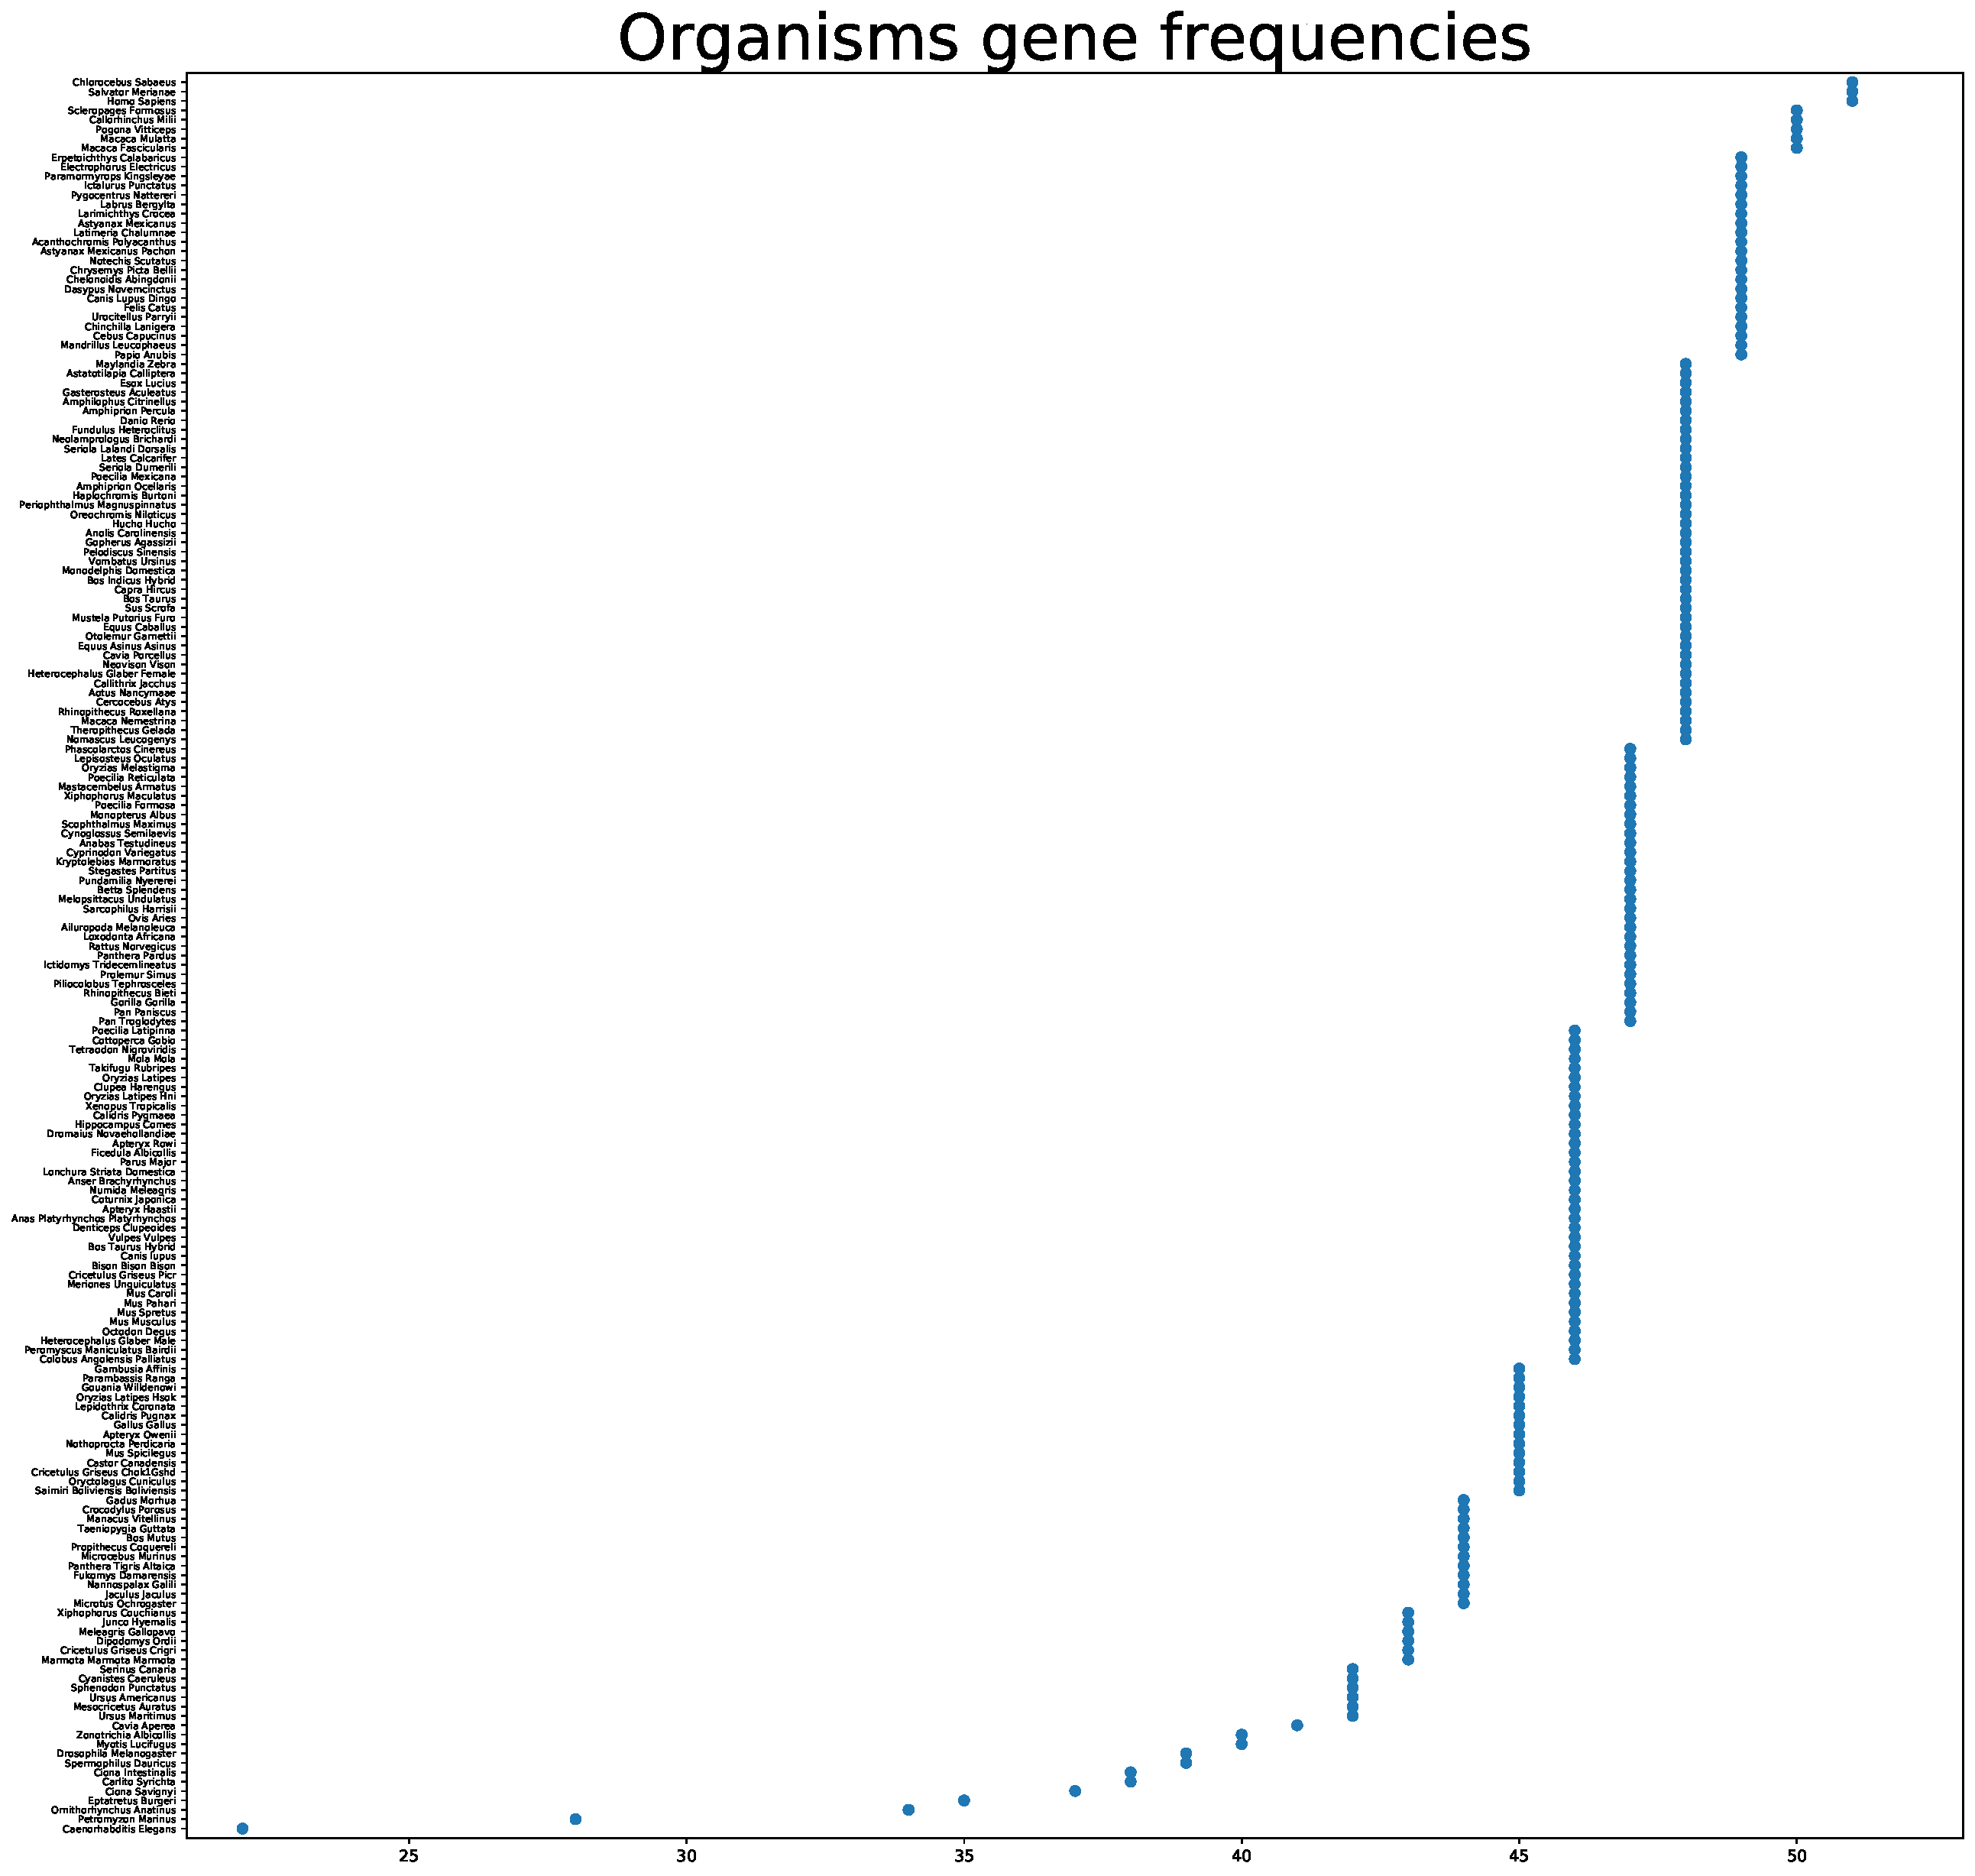
\includegraphics[height=6in,trim={0 0 0 0.628in},clip]{./appendix_images/gene_frequencies.pdf}}
\caption{\textbf{A plot of gene organisms vs. gene frequencies.} The organisms were sorted in ascending order based on the number of genes their genomes include out of the 51 gene present in the proteoglycan synthesis pathway.}
\label{sup_fig_1}
\end{figure}

\begin{figure}[H]
\centering
\makebox[\textwidth][c]{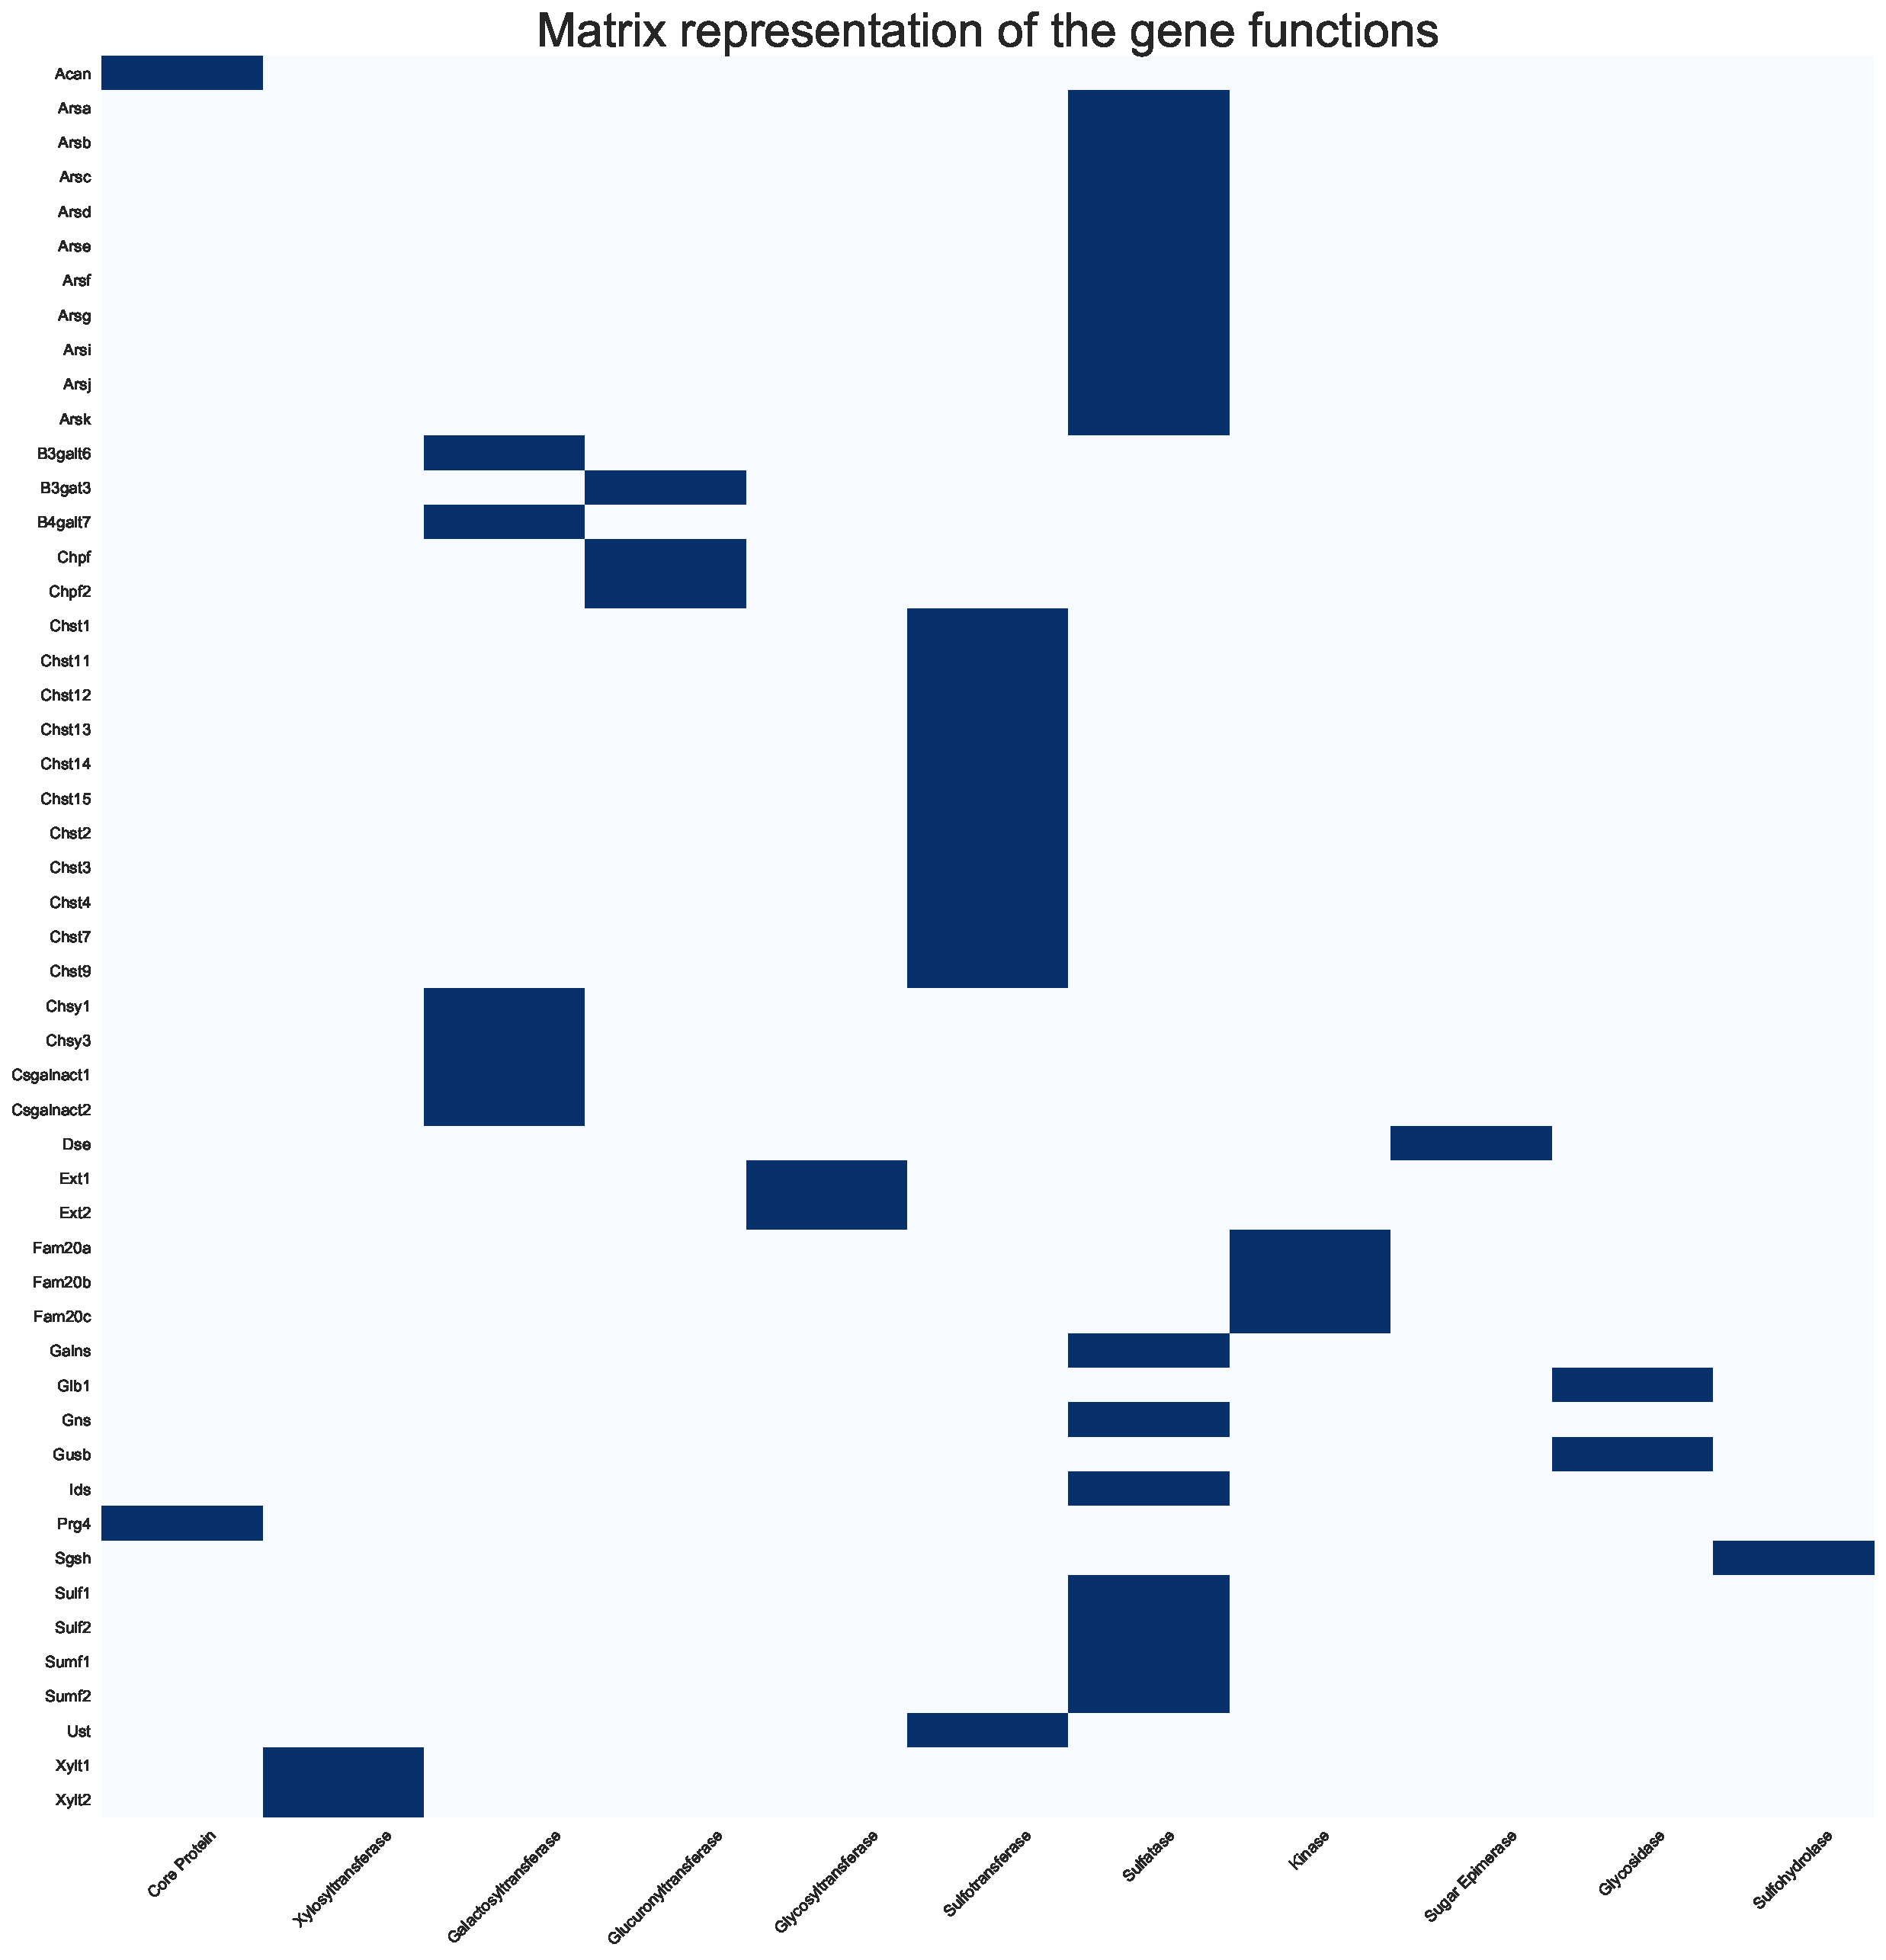
\includegraphics[height=7in,trim={0 0 0 0.5in},clip]{./appendix_images/gene_functions.pdf}}
\caption{\textbf{A matrix representation of gene function.} Gene are plotted against known functions. Dark blue coloured cells indicate that gene on axis y performs the corresponding x axis function.}
\label{sup_fig_2}
\end{figure}

\begin{figure}[H]
\centering
\makebox[\textwidth][c]{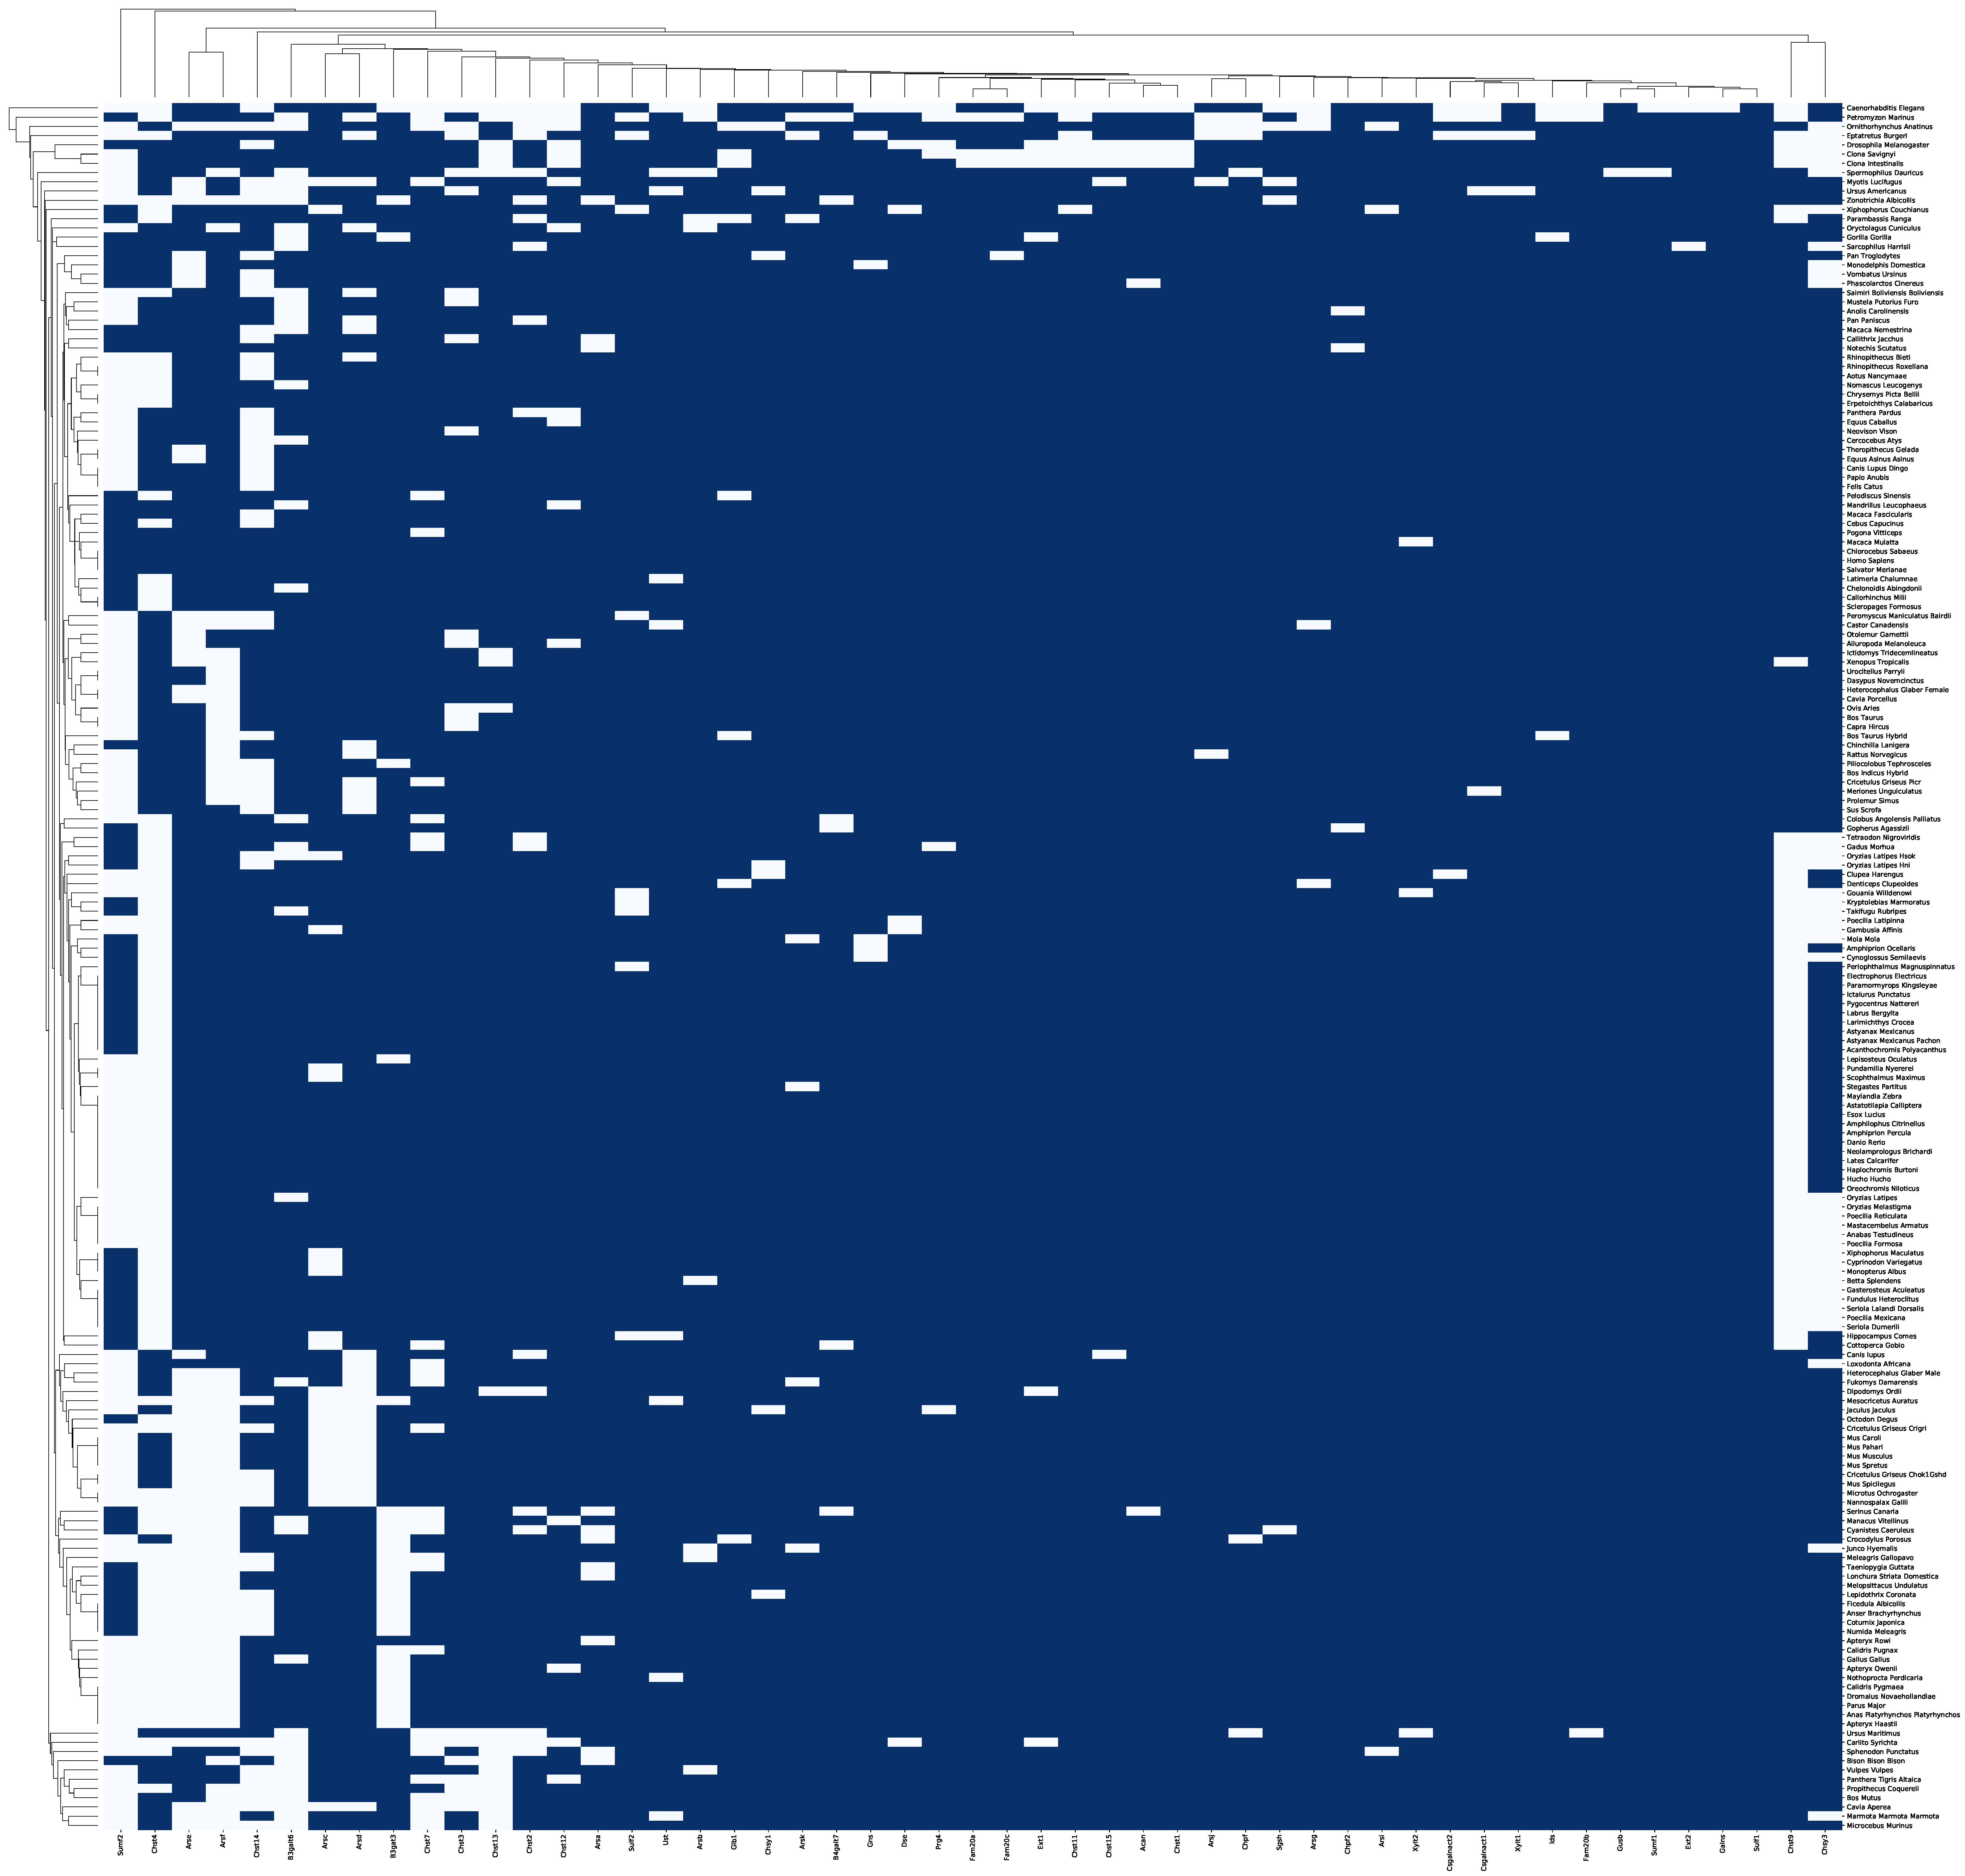
\includegraphics[height=7in,trim={0 0 0 0in},clip]{./appendix_images/genes_clustermap.pdf}}
\caption{\textbf{A clustermap of organisms vs. genes.} Dark blue coloured cells indicate that the genome of the organism listed on the y axis contains the corresponding gene on the x axis. Organisms were clustered based on gene presence using the Euclidean distance between binary vectors indicating what genes are present in a specific genome.}
\label{sup_fig_3}
\end{figure}

\newpage
\section{Phylogeny}
This section includes supplementary material generated for visualizing paired phylogenetic trees. 

\begin{figure}[H]
\centering
\makebox[\textwidth][c]{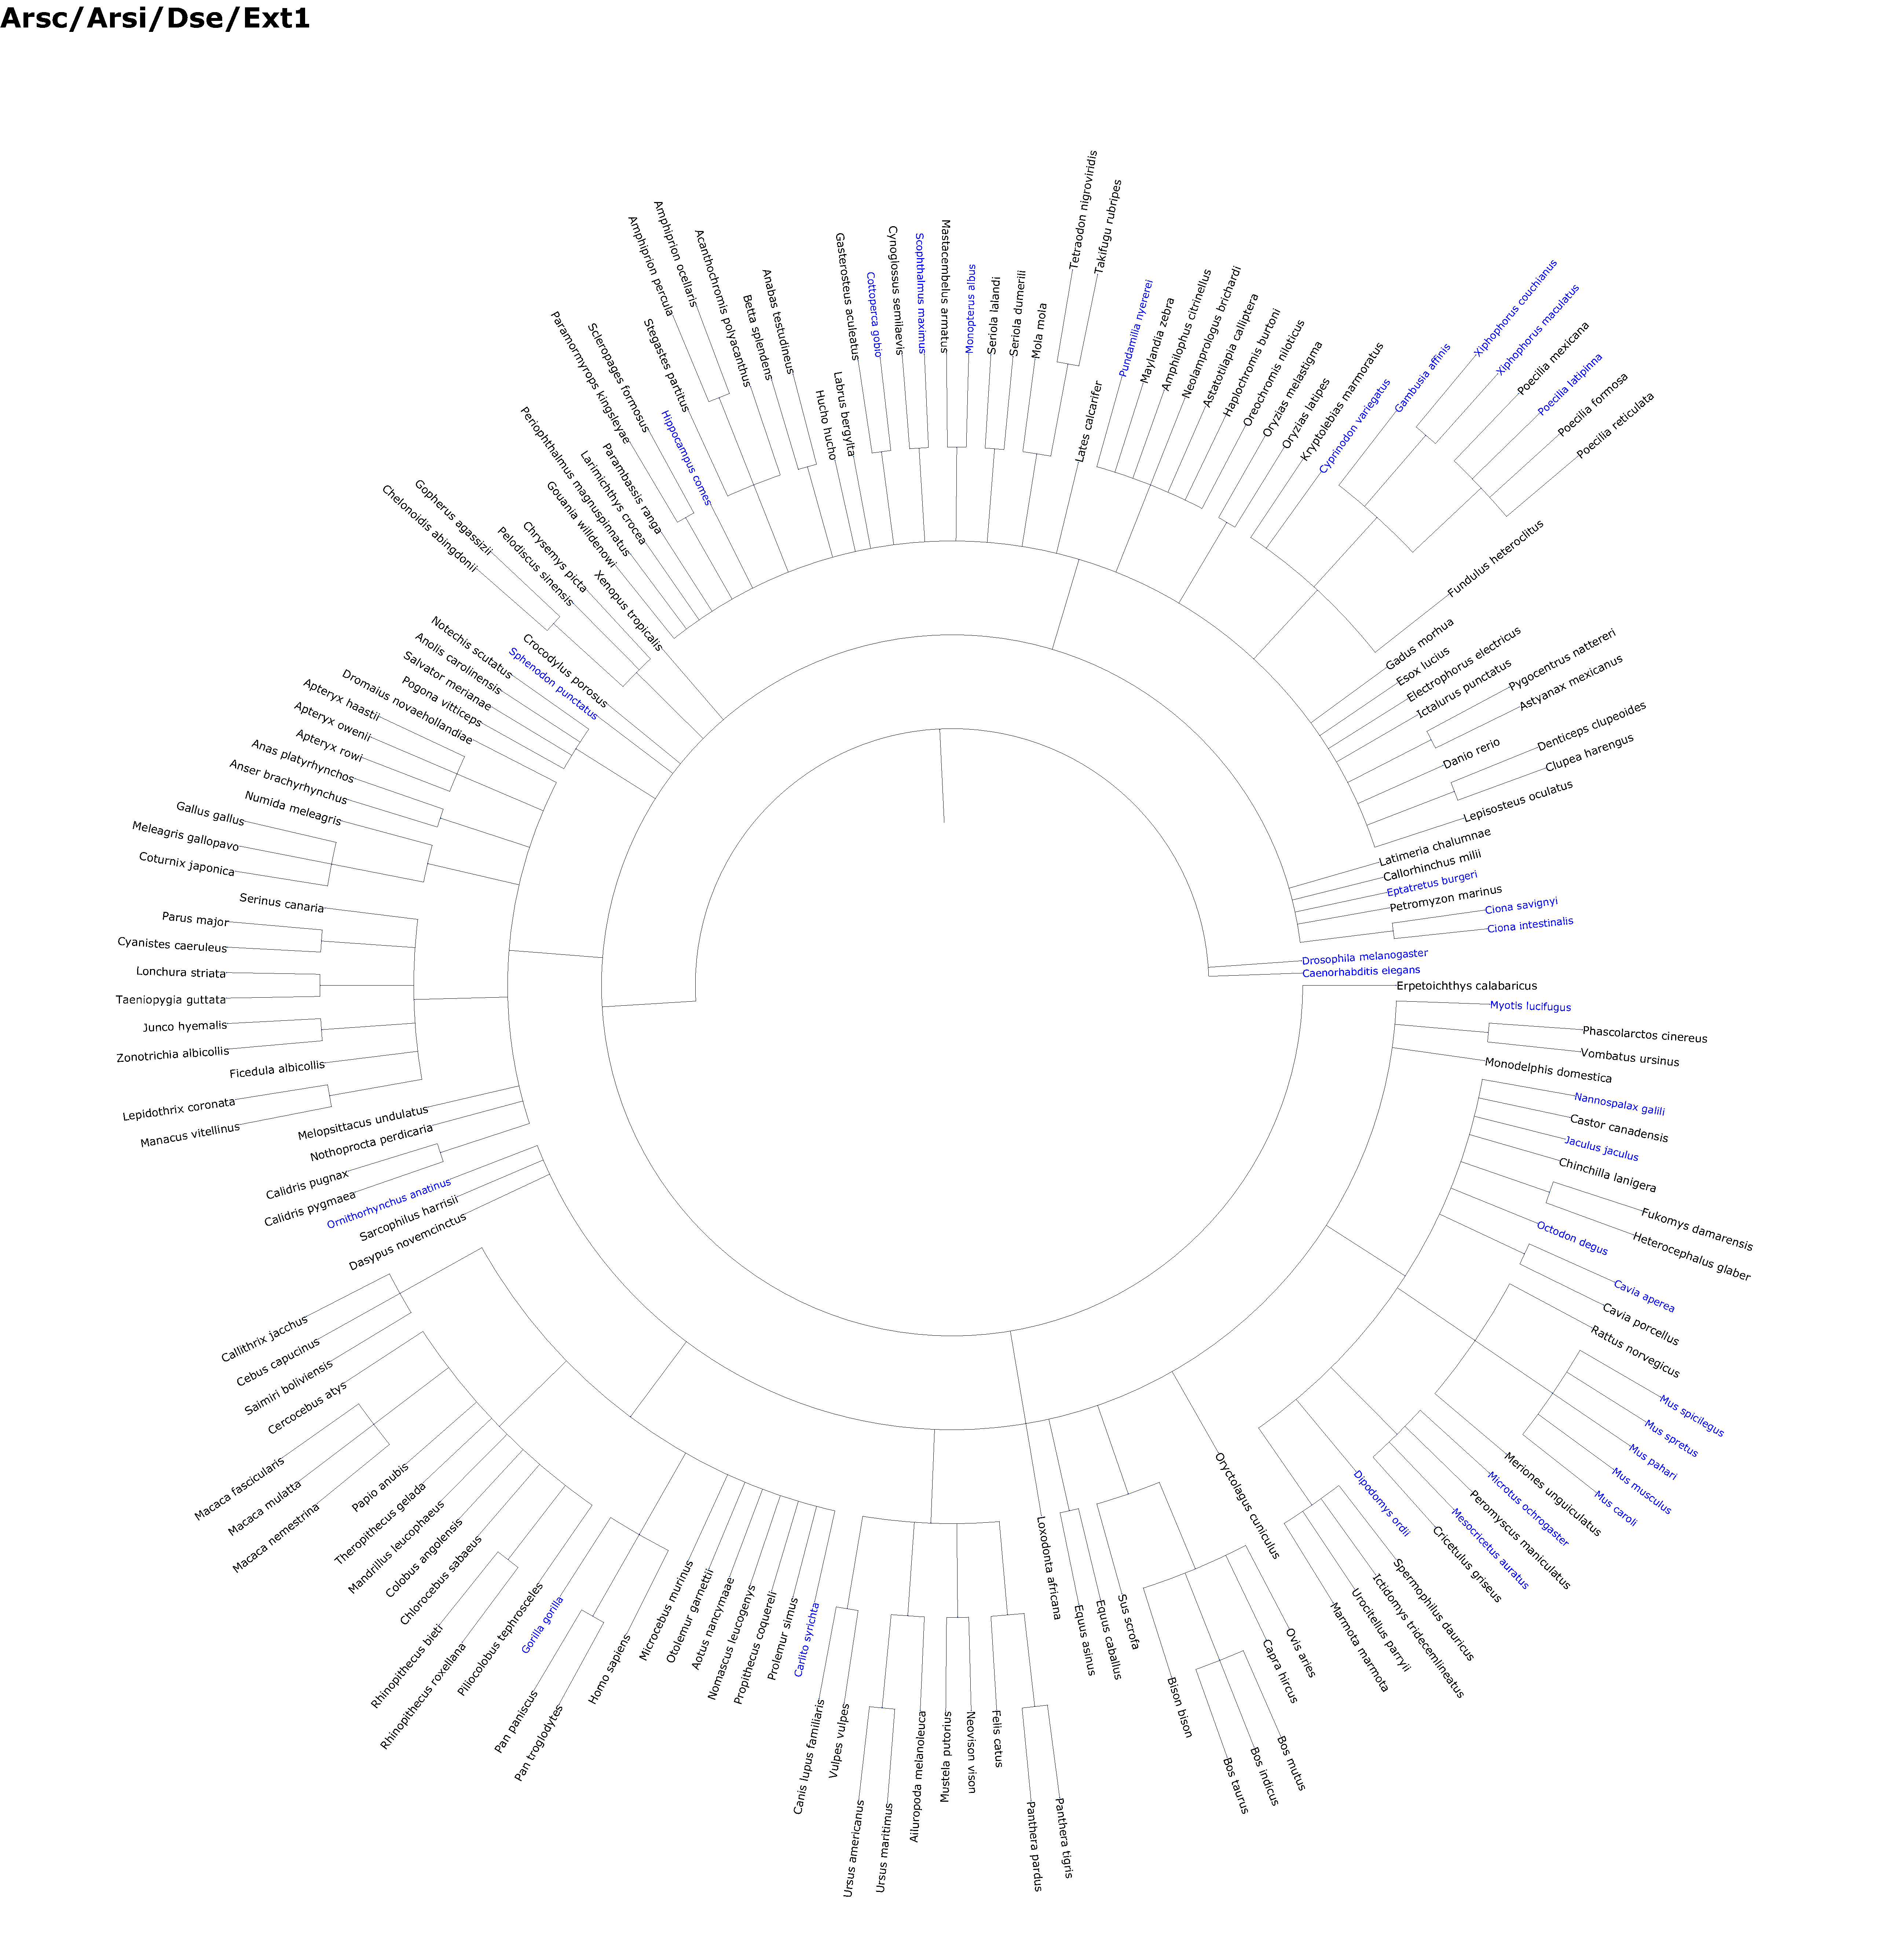
\includegraphics[height=6.5in,trim={0 0 0 3in},clip]{./appendix_images/trees/Arsc_Arsi_Dse_Ext1.pdf}}
\caption{\textbf{The paired gene tree for \textit{Arsc, Arsi, Dse}, and \textit{Ext1}.}}
\label{sup_fig_4}
\end{figure}

\begin{figure}[H]
\centering
\makebox[\textwidth][c]{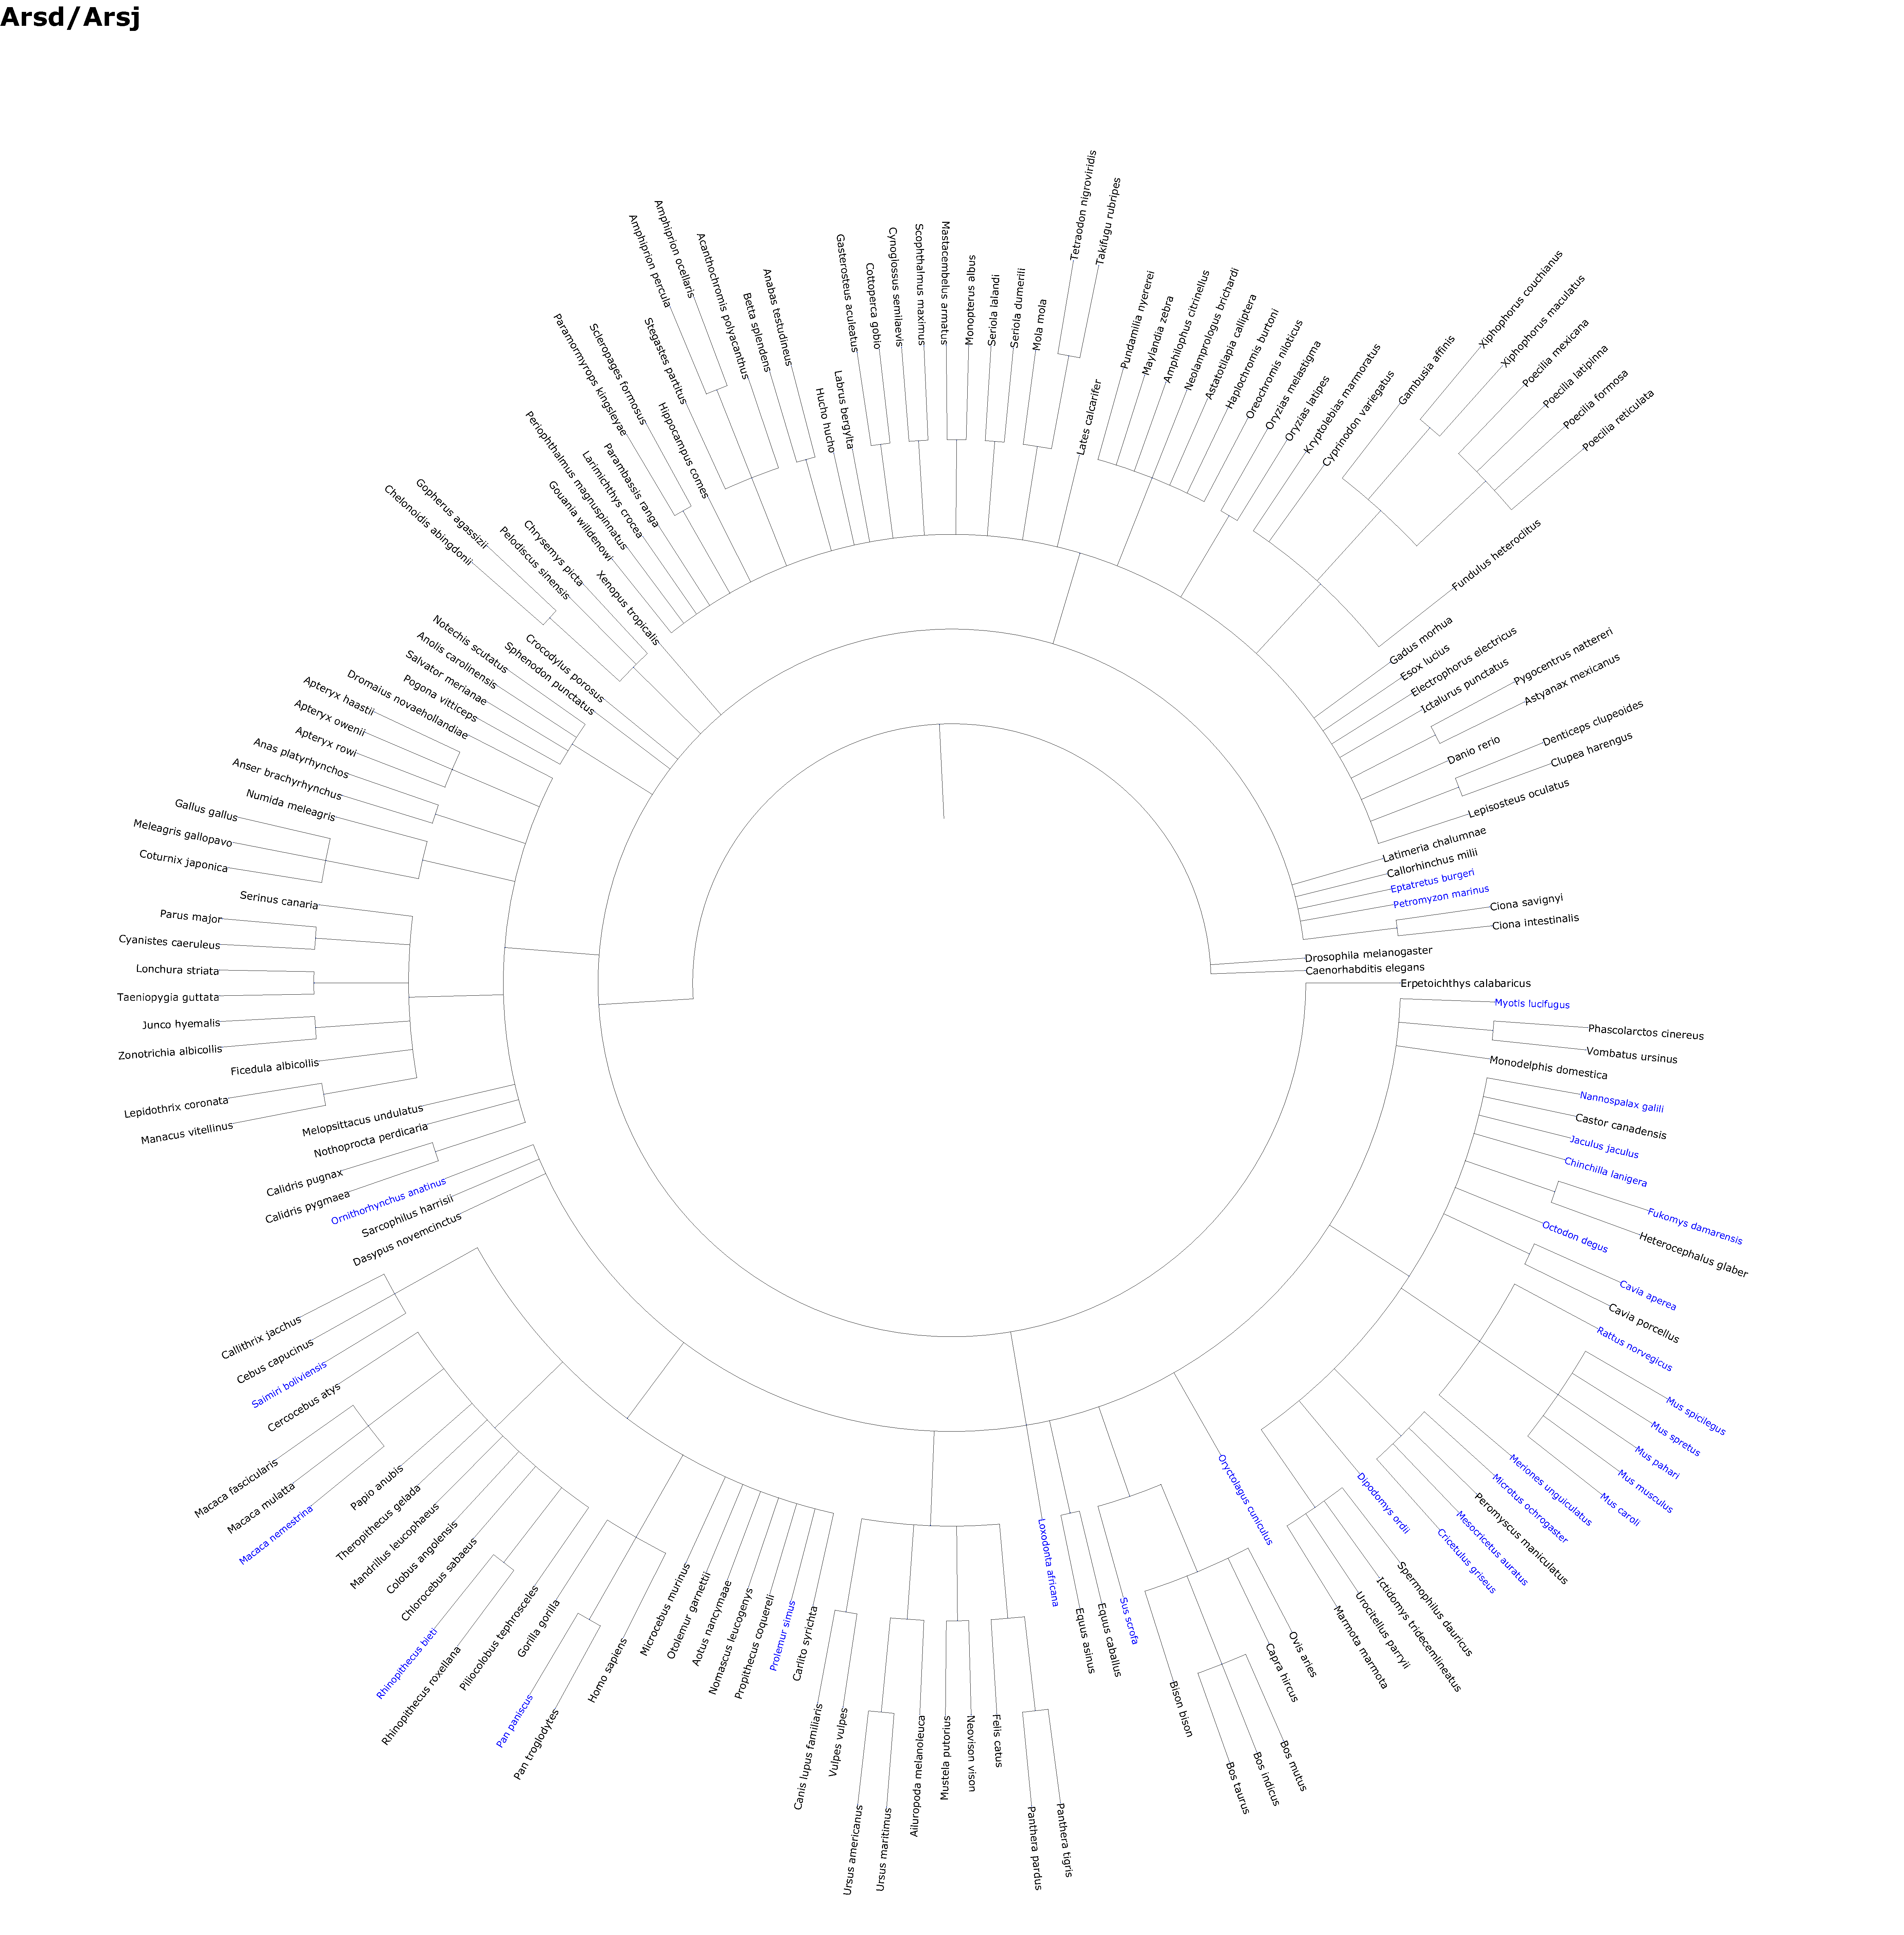
\includegraphics[height=7in,trim={0 0 0 3in},clip]{./appendix_images/trees/Arsd_Arsj.pdf}}
\caption{\textbf{The paired gene tree for \textit{Arsd}, and \textit{Arsj}.}}
\label{sup_fig_5}
\end{figure}

\begin{figure}[H]
\centering
\makebox[\textwidth][c]{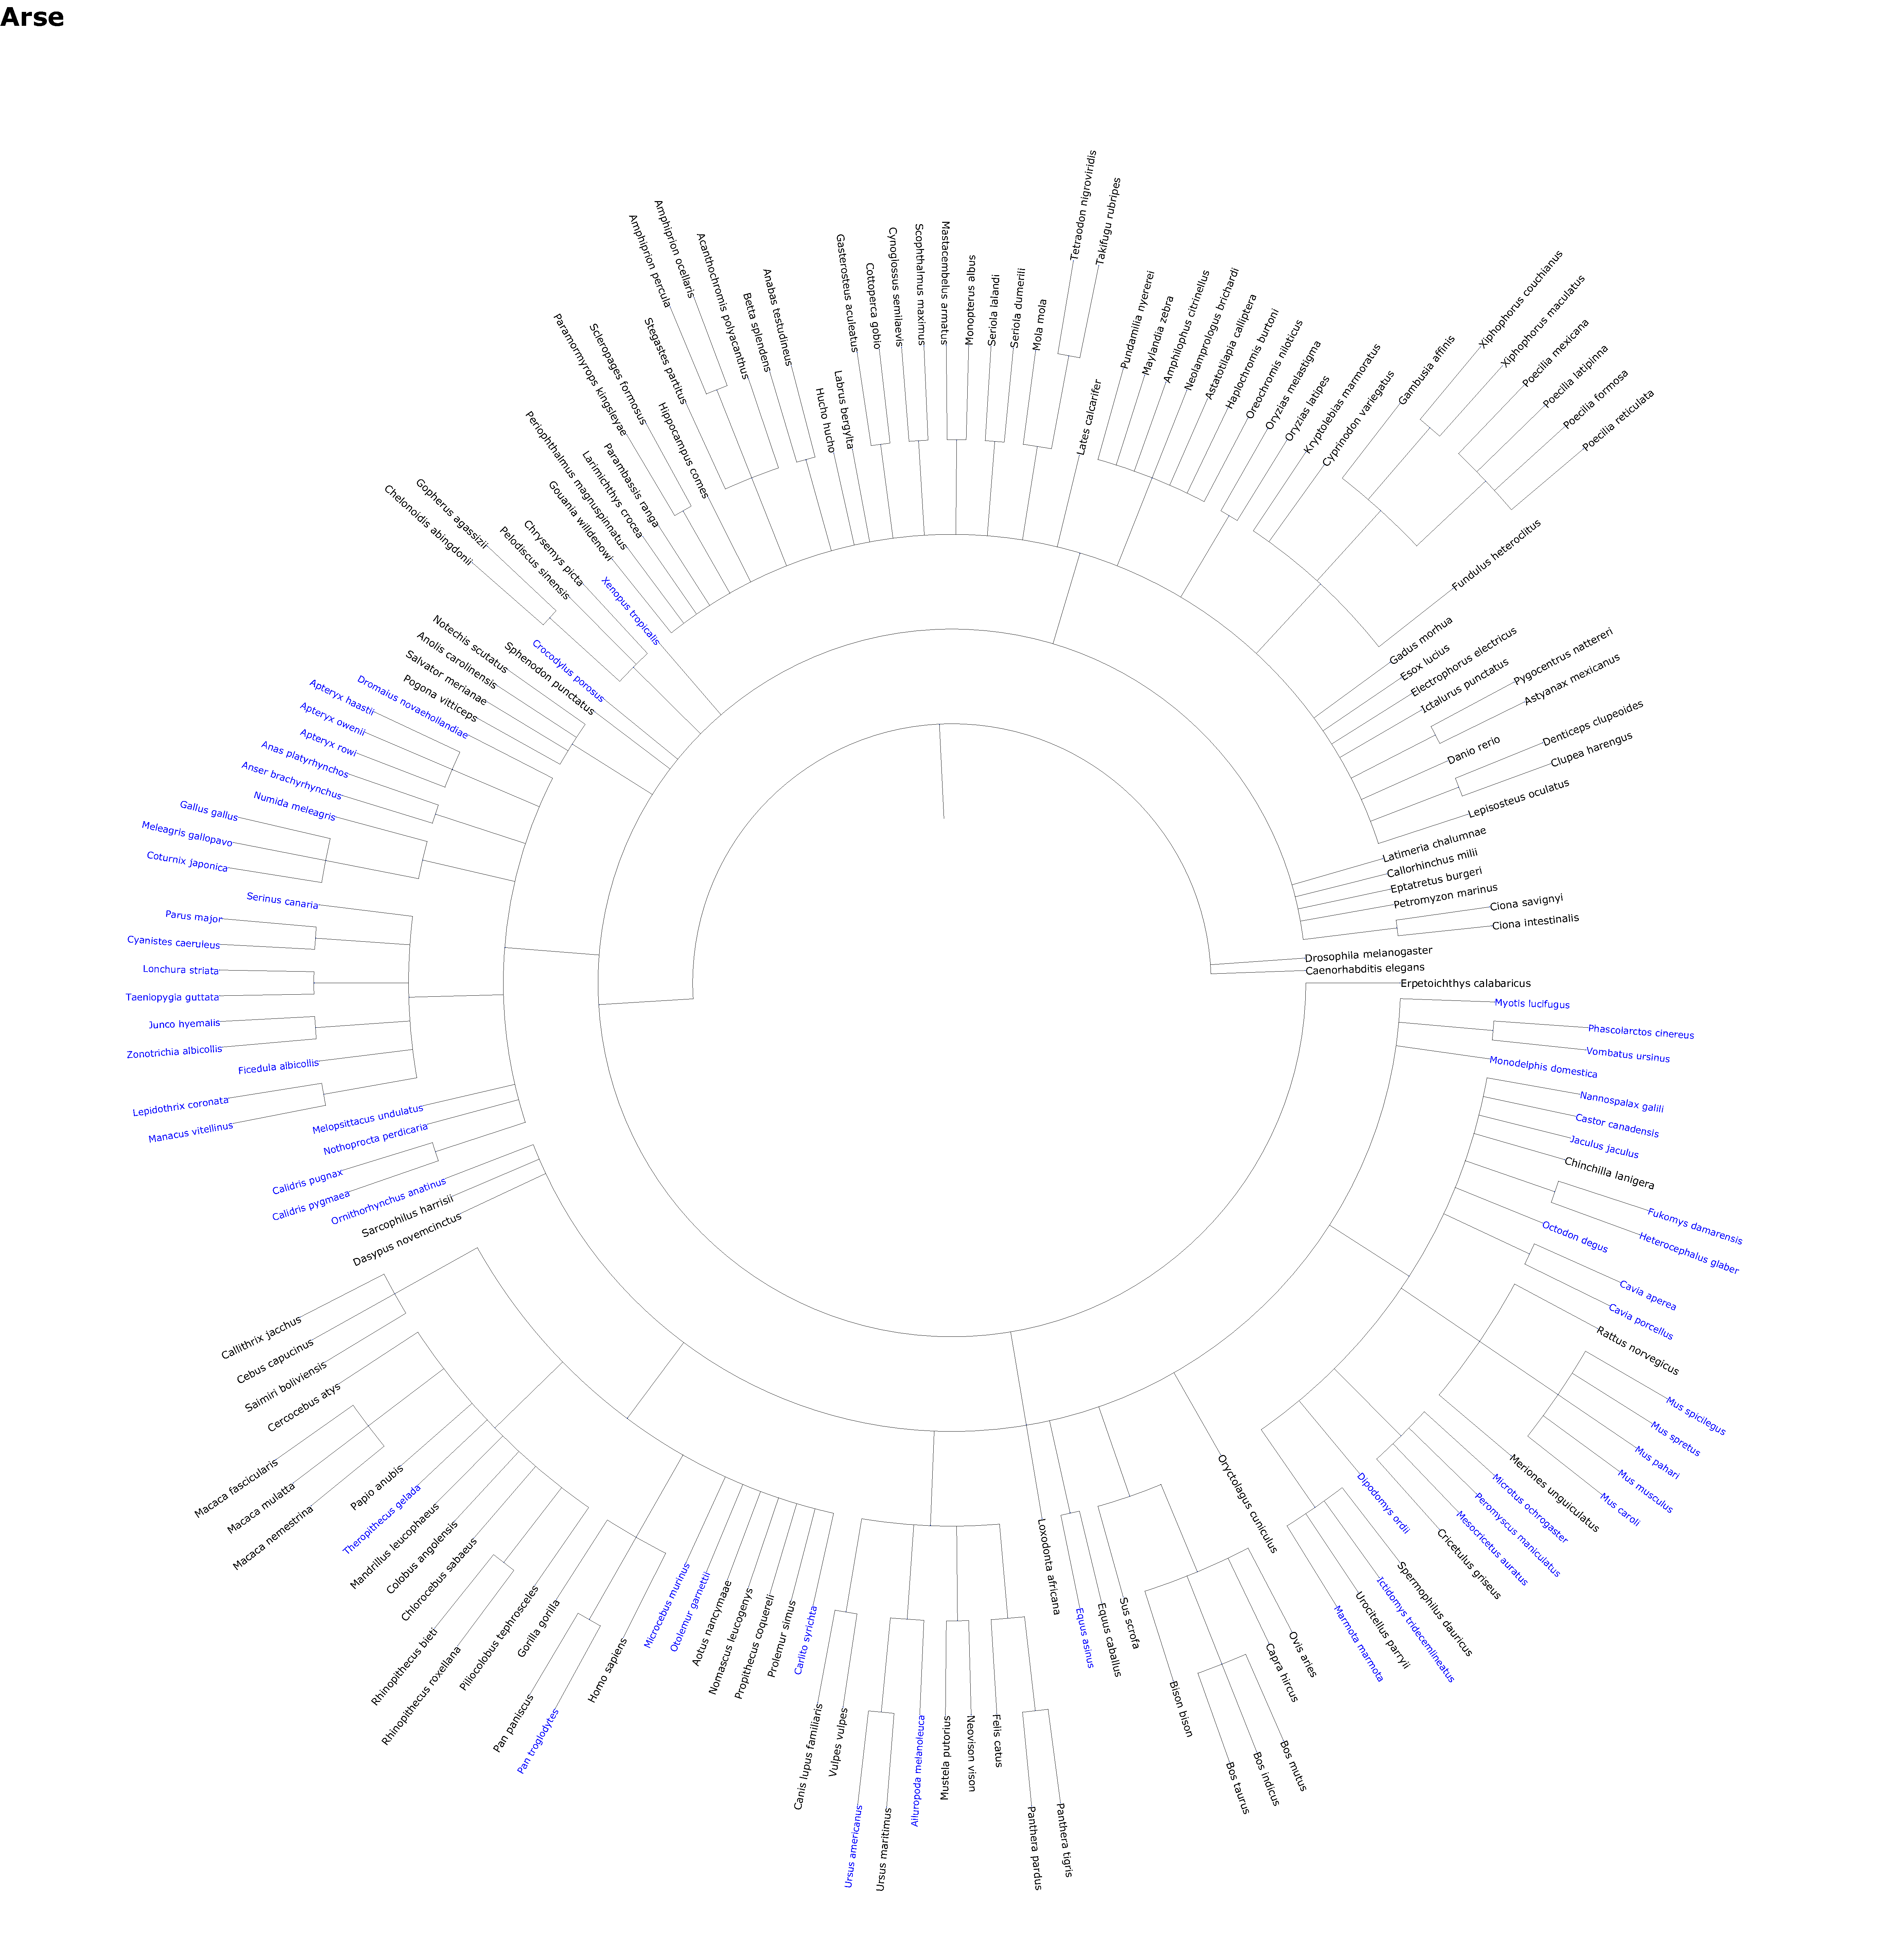
\includegraphics[height=7in,trim={0 0 0 3in},clip]{./appendix_images/trees/Arse.pdf}}
\caption{\textbf{The gene tree for \textit{Arse}.}}
\label{sup_fig_6}
\end{figure}

\begin{figure}[H]
\centering
\makebox[\textwidth][c]{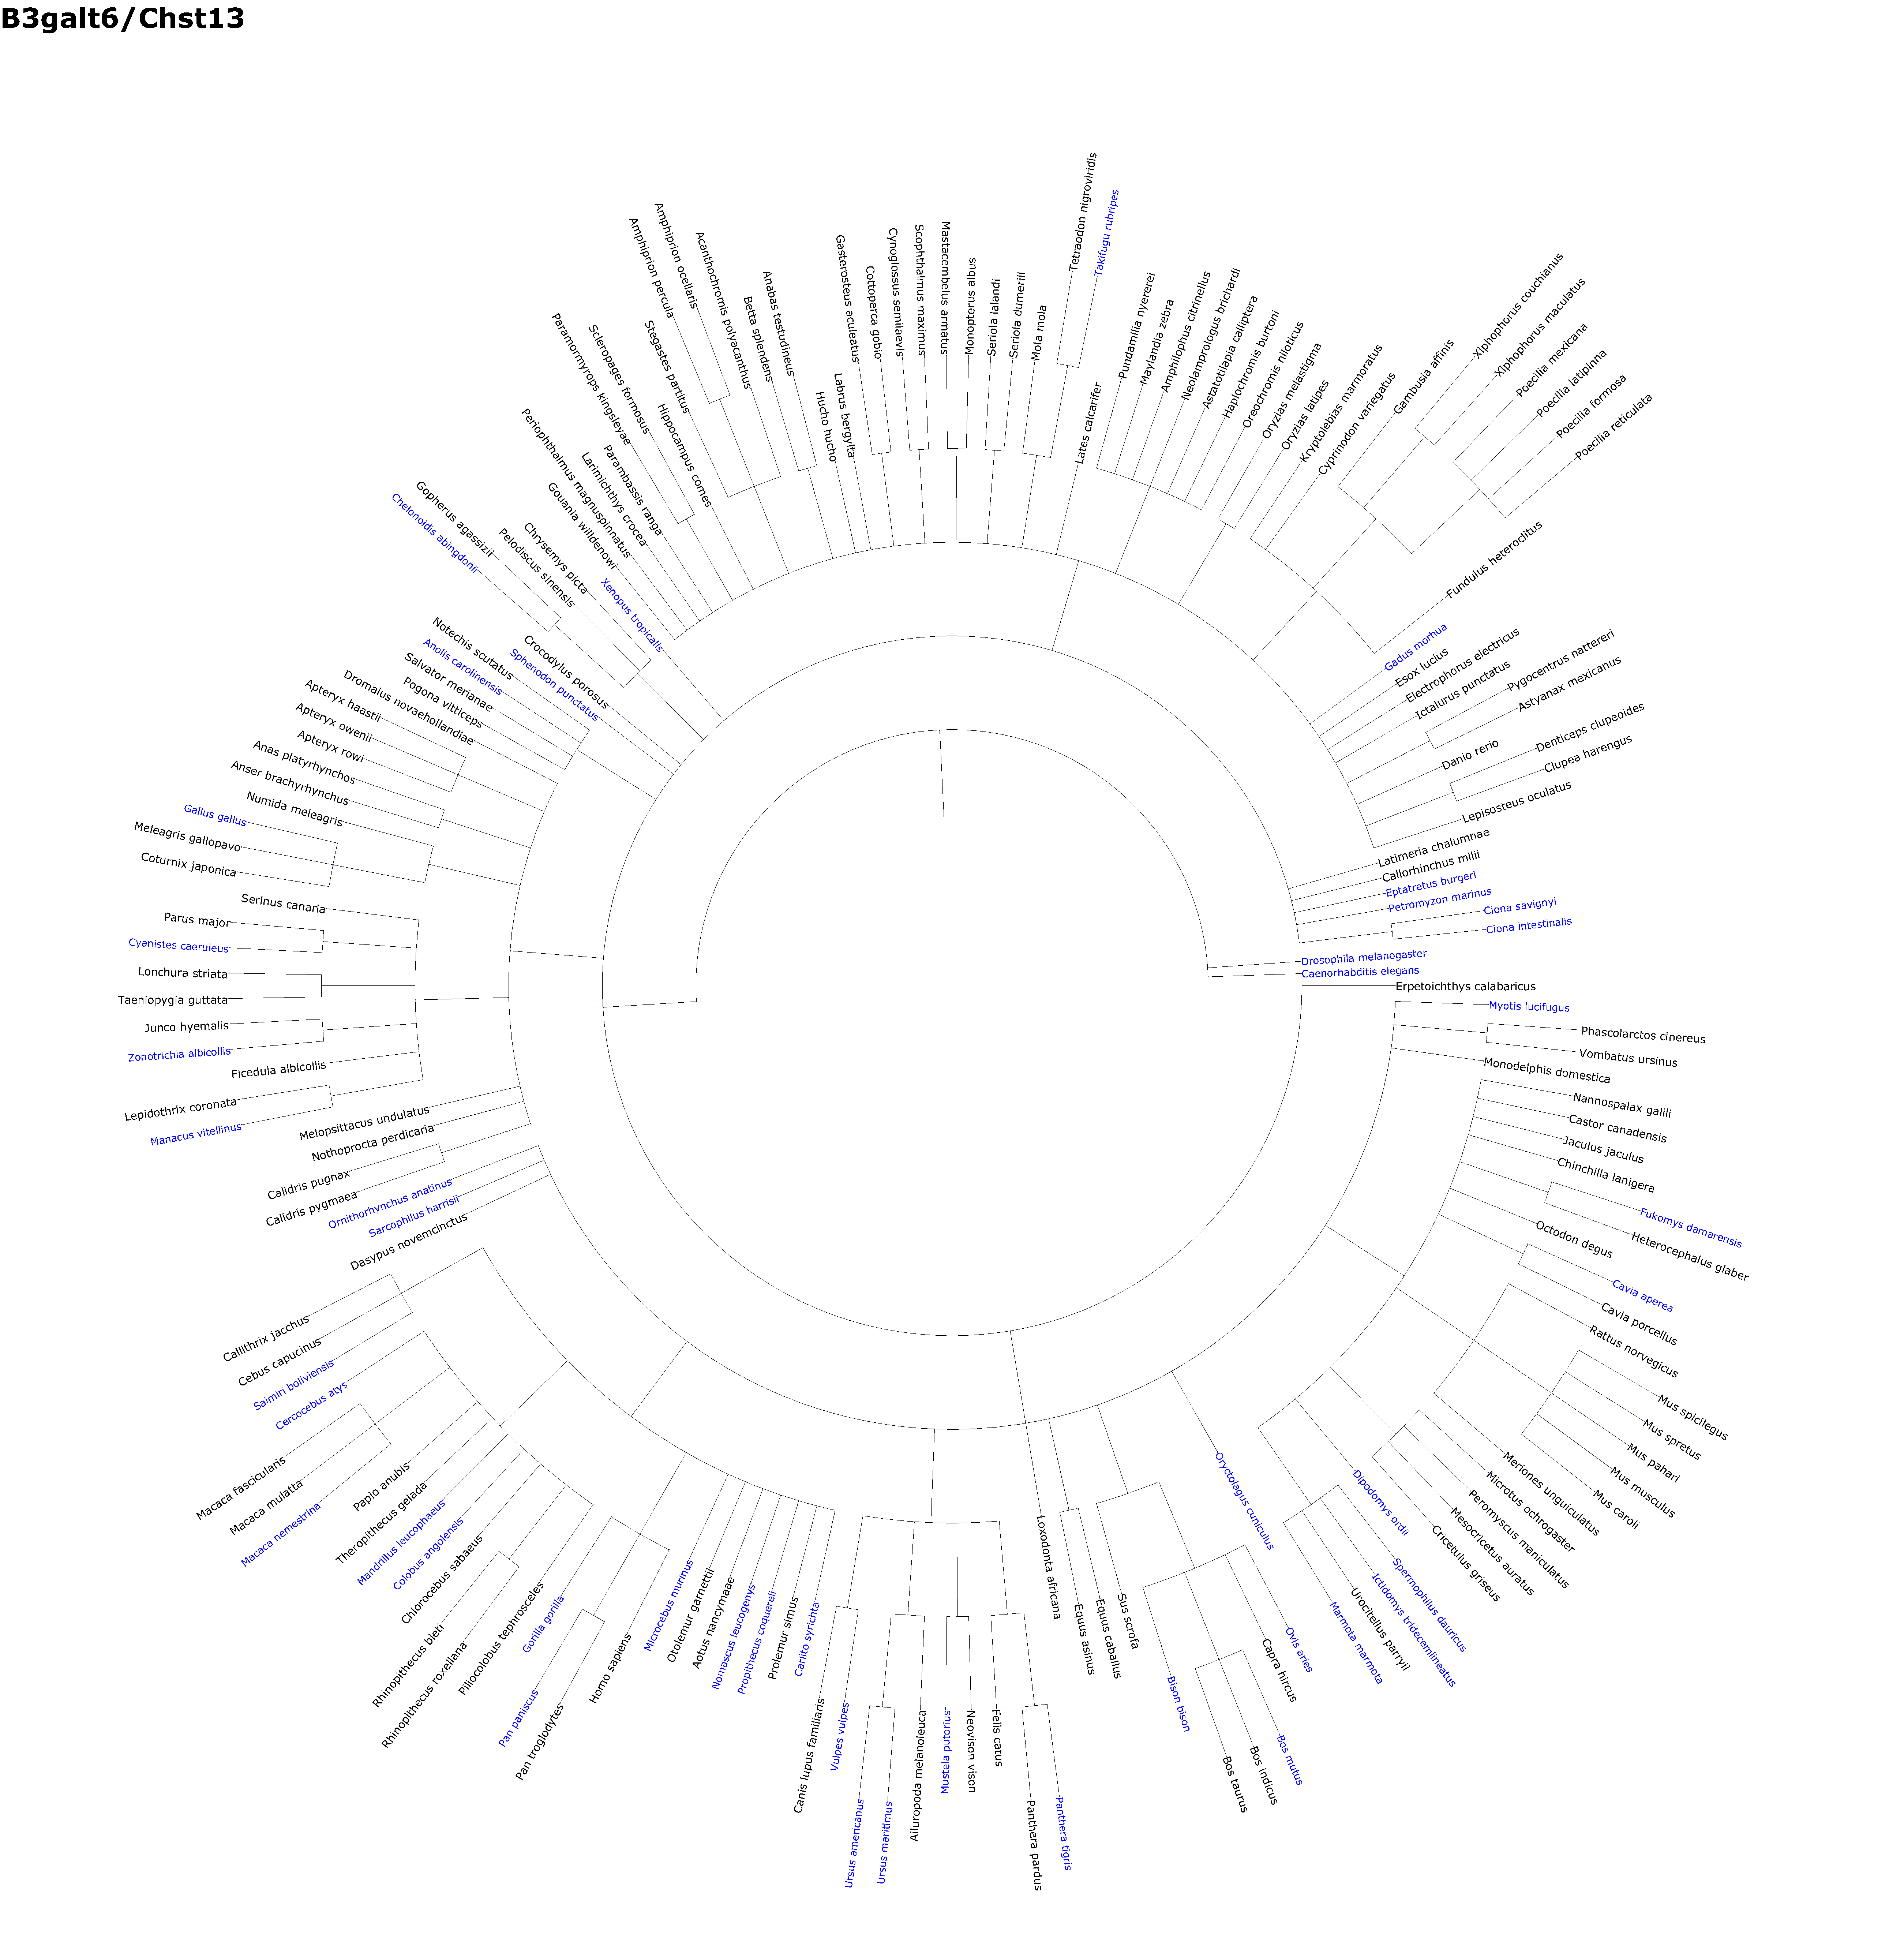
\includegraphics[height=7in,trim={0 0 0 3in},clip]{./appendix_images/trees/B3galt6_Chst13.pdf}}
\caption{\textbf{The gene tree for \textit{B3galt6} and \textit{Chst13}.}}
\label{sup_fig_7}
\end{figure}

\begin{figure}[H]
\centering
\makebox[\textwidth][c]{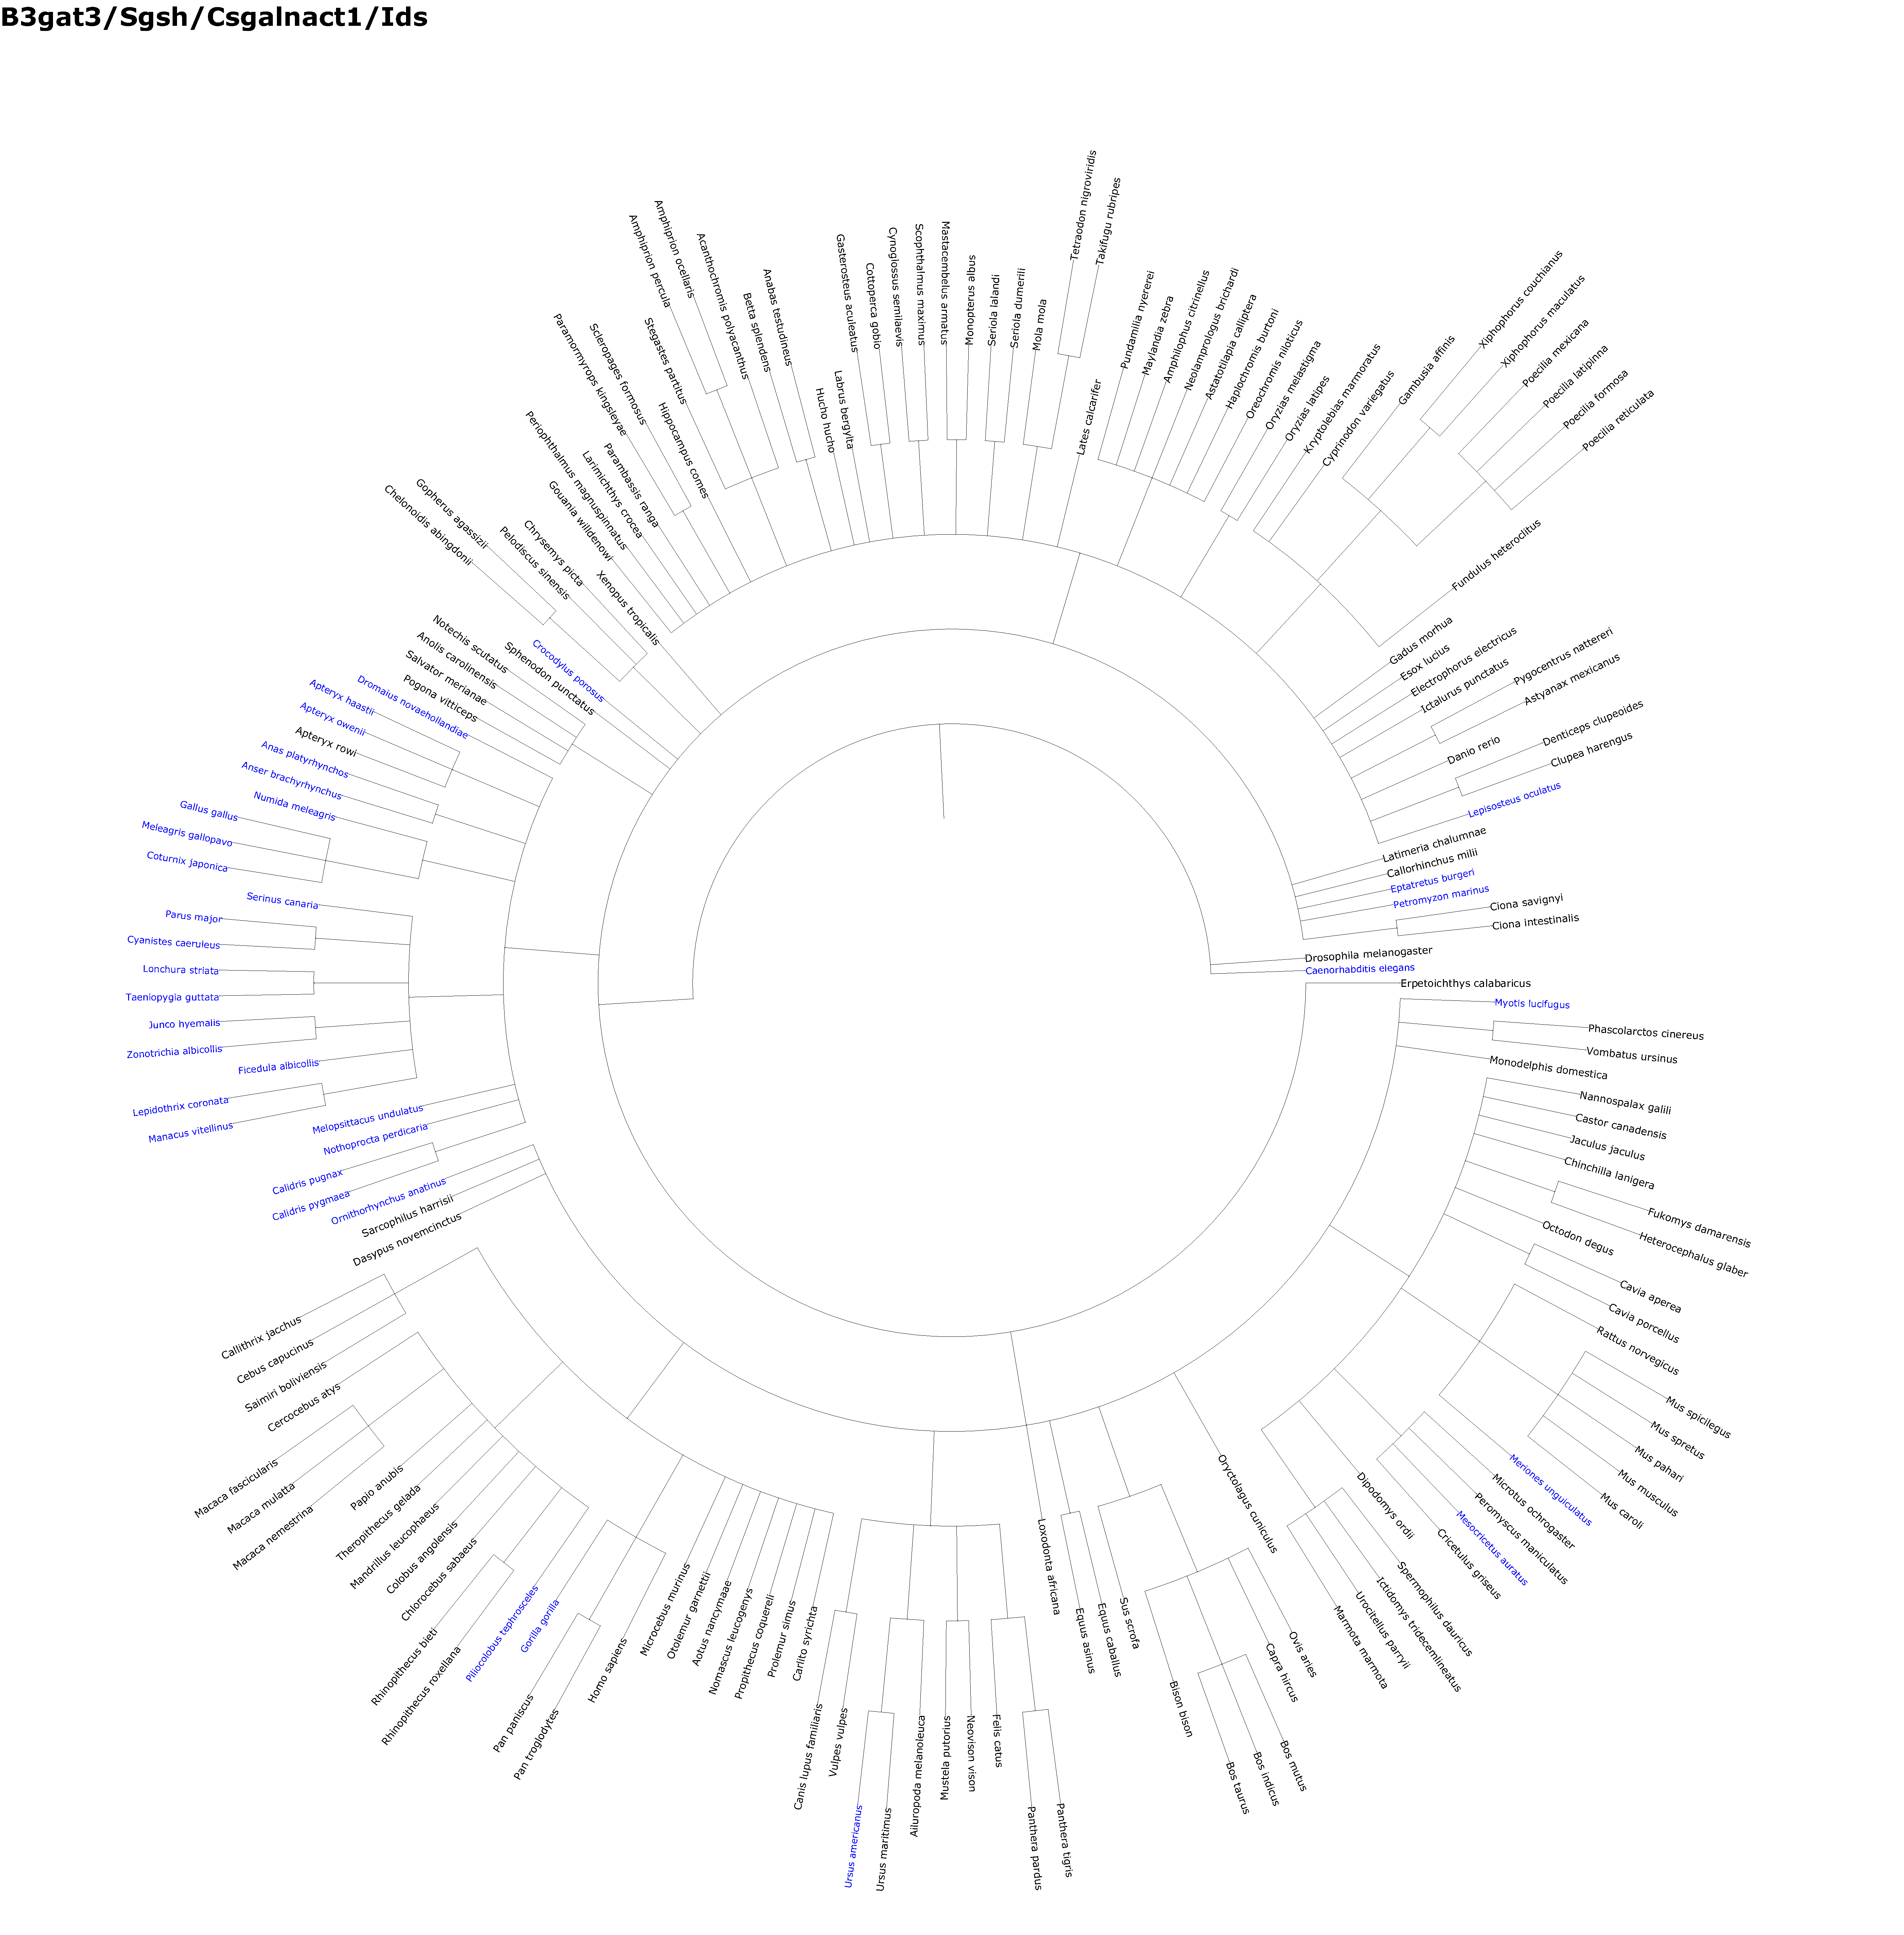
\includegraphics[height=7in,trim={0 0 0 3in},clip]{./appendix_images/trees/B3gat3_Sgsh_Csgalnact1_Ids.pdf}}
\caption{\textbf{The gene tree for \textit{B3gat6, Sgsh, Csgalnact1} and \textit{Ids}.}}
\label{sup_fig_8}
\end{figure}

\begin{figure}[H]
\centering
\makebox[\textwidth][c]{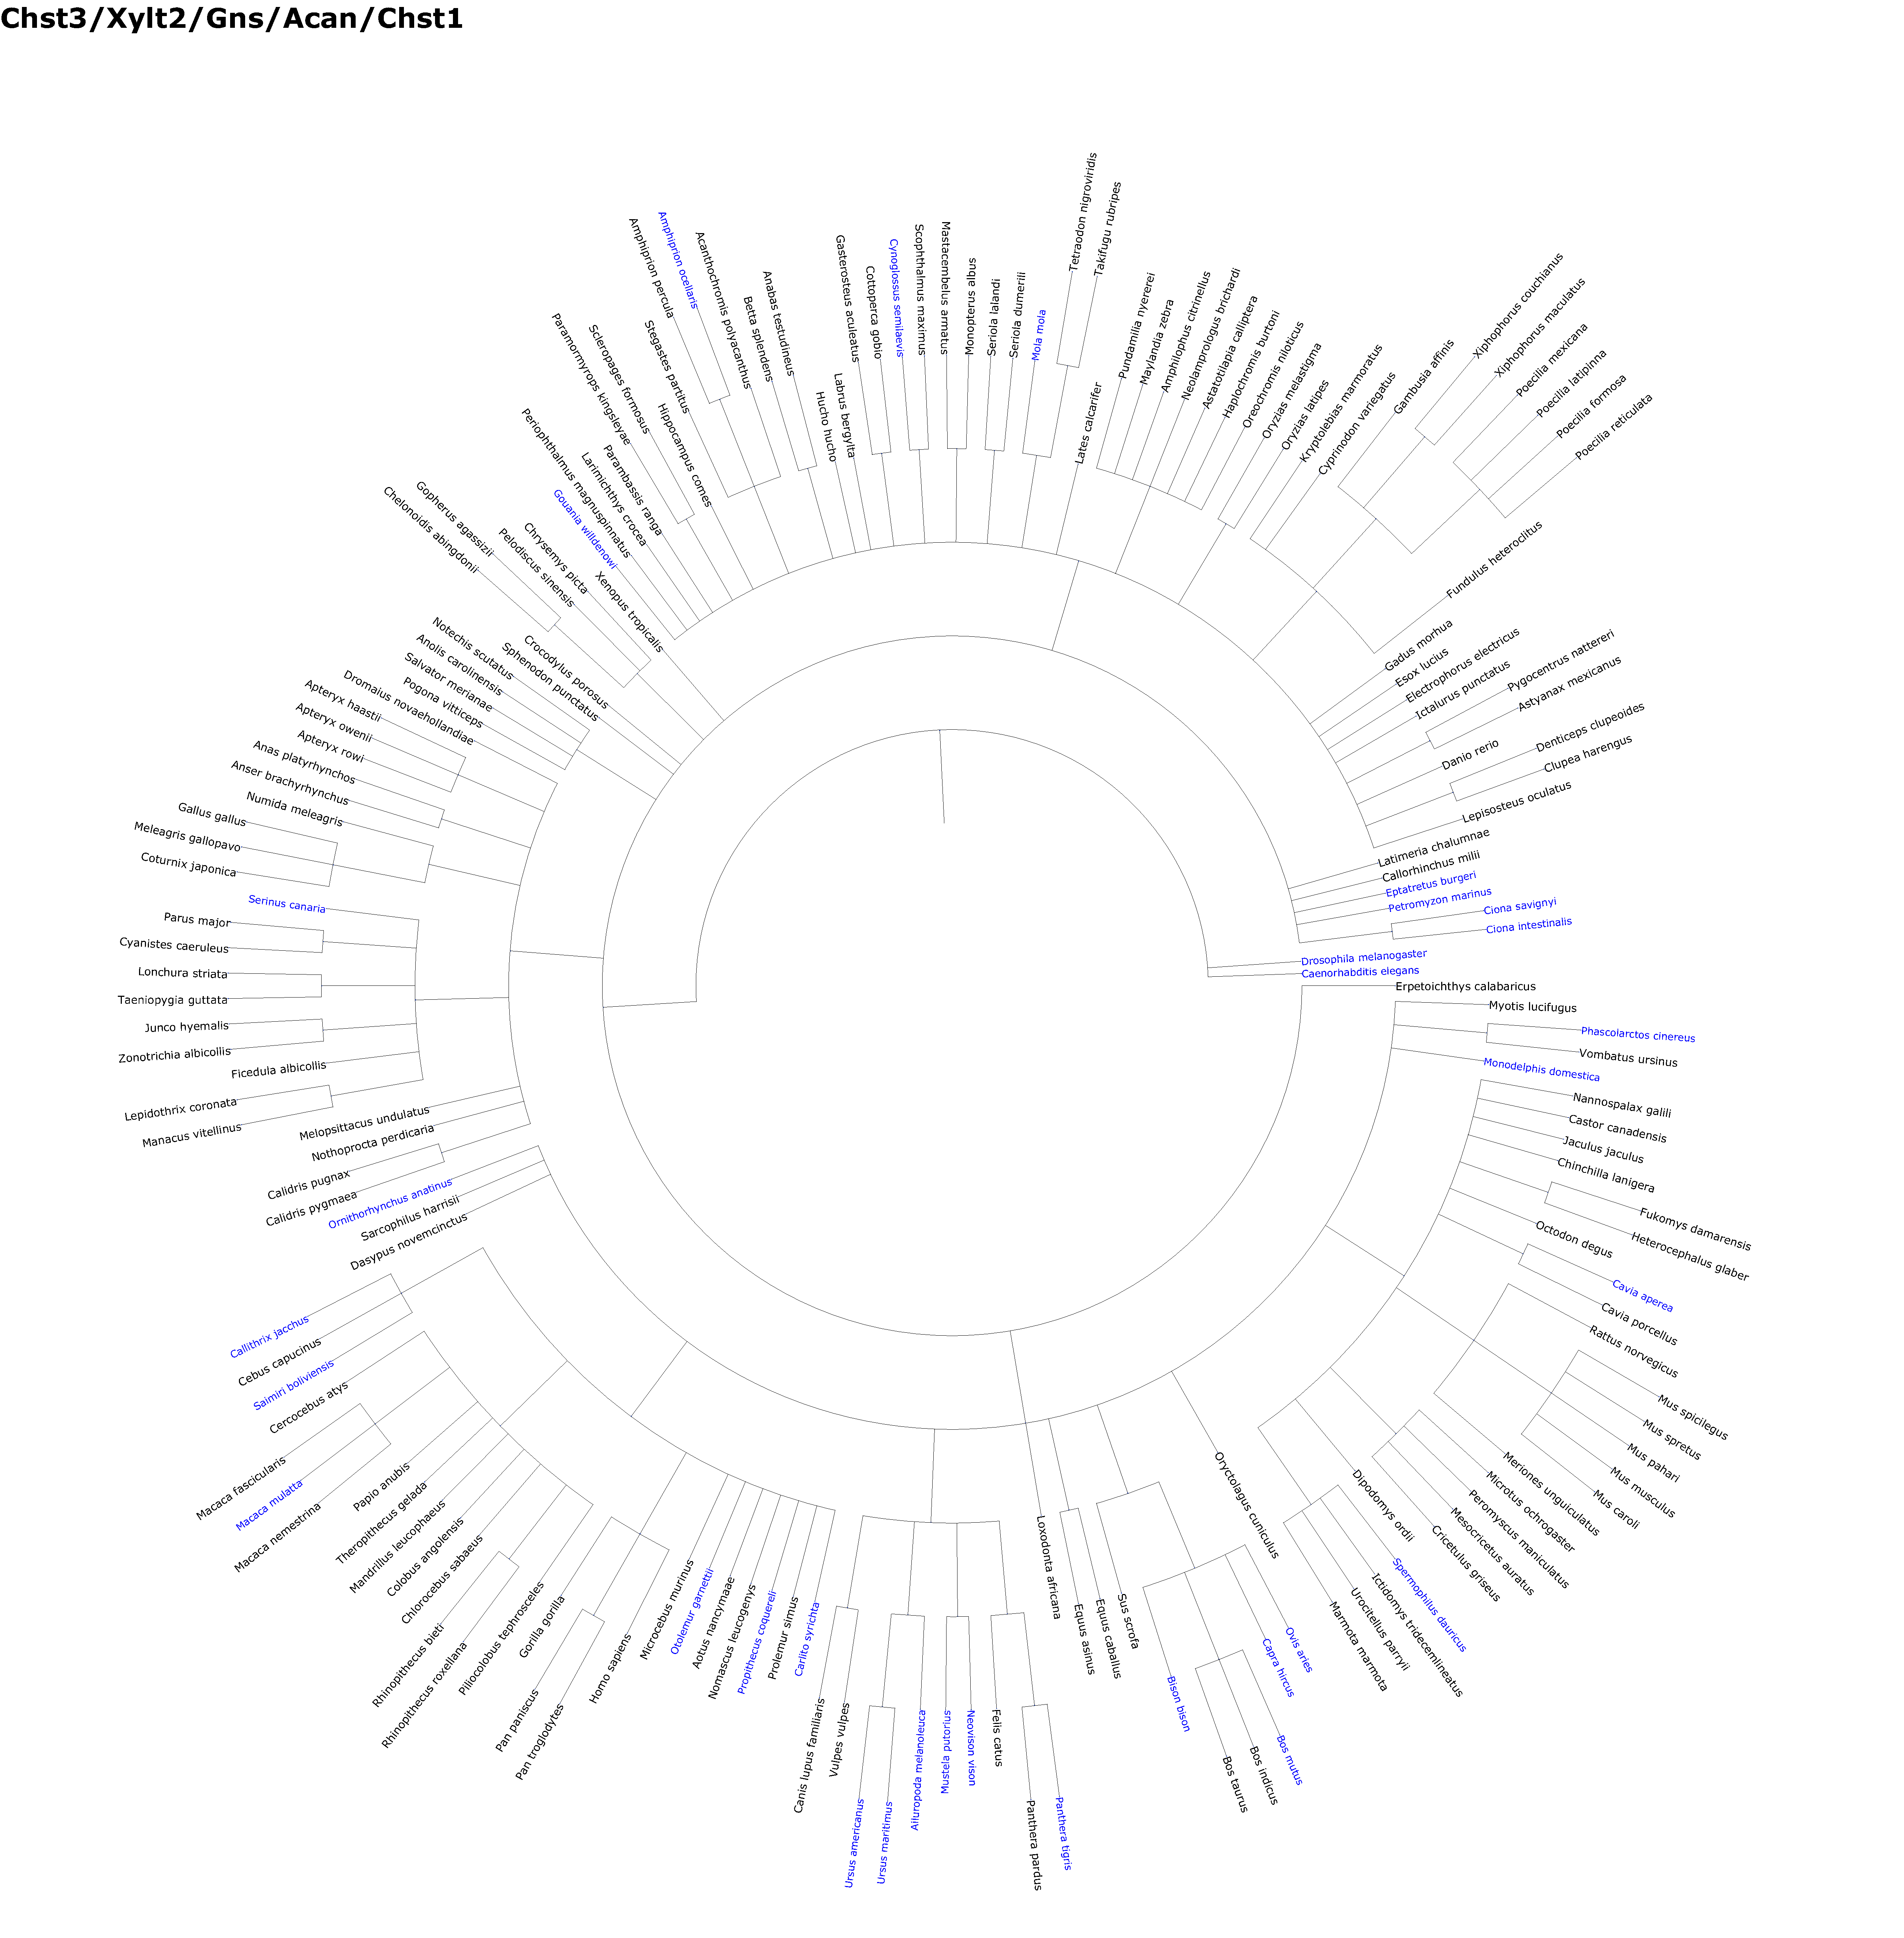
\includegraphics[height=7in,trim={0 0 0 3in},clip]{./appendix_images/trees/Chst3_Xylt2_Gns_Acan_Chst1.pdf}}
\caption{\textbf{The gene tree for \textit{Chst3, Xylt2, Gns, Acan} and \textit{Chst1}.}}
\label{sup_fig_9}
\end{figure}

\begin{figure}[H]
\centering
\makebox[\textwidth][c]{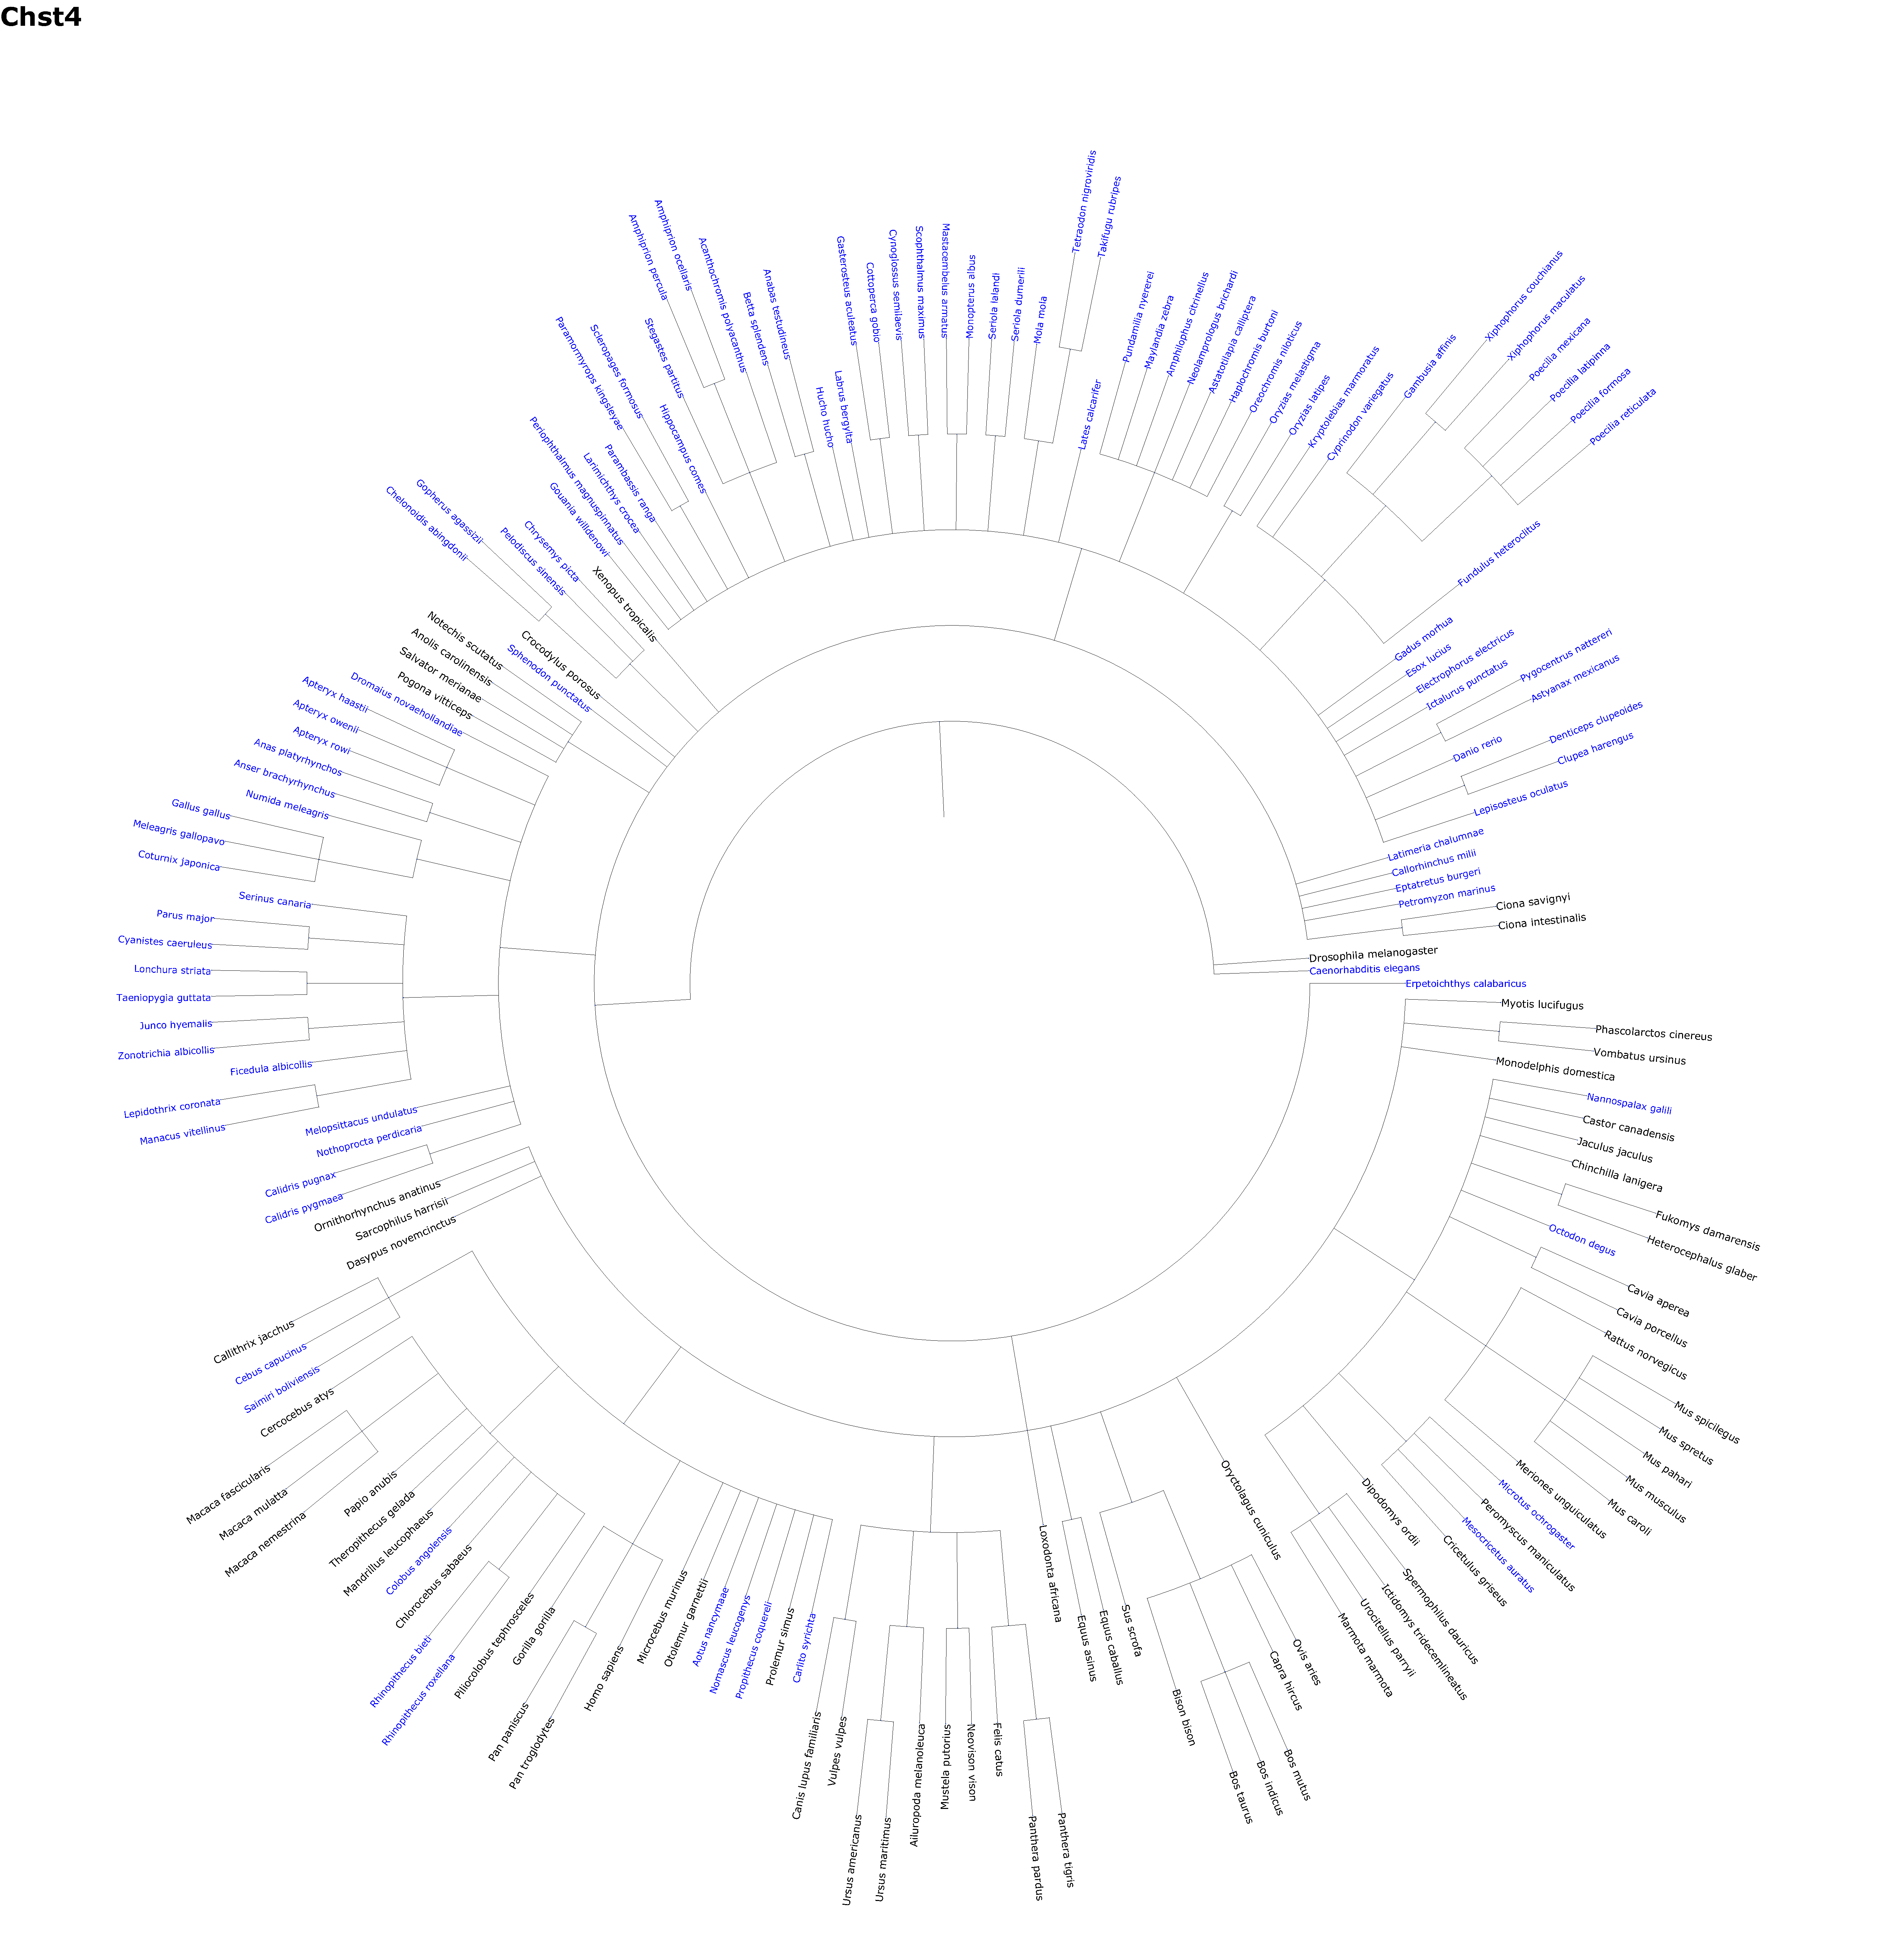
\includegraphics[height=7in,trim={0 0 0 3in},clip]{./appendix_images/trees/Chst4.pdf}}
\caption{\textbf{The gene tree for \textit{Chst4.}}}
\label{sup_fig_10}
\end{figure}

\begin{figure}[H]
\centering
\makebox[\textwidth][c]{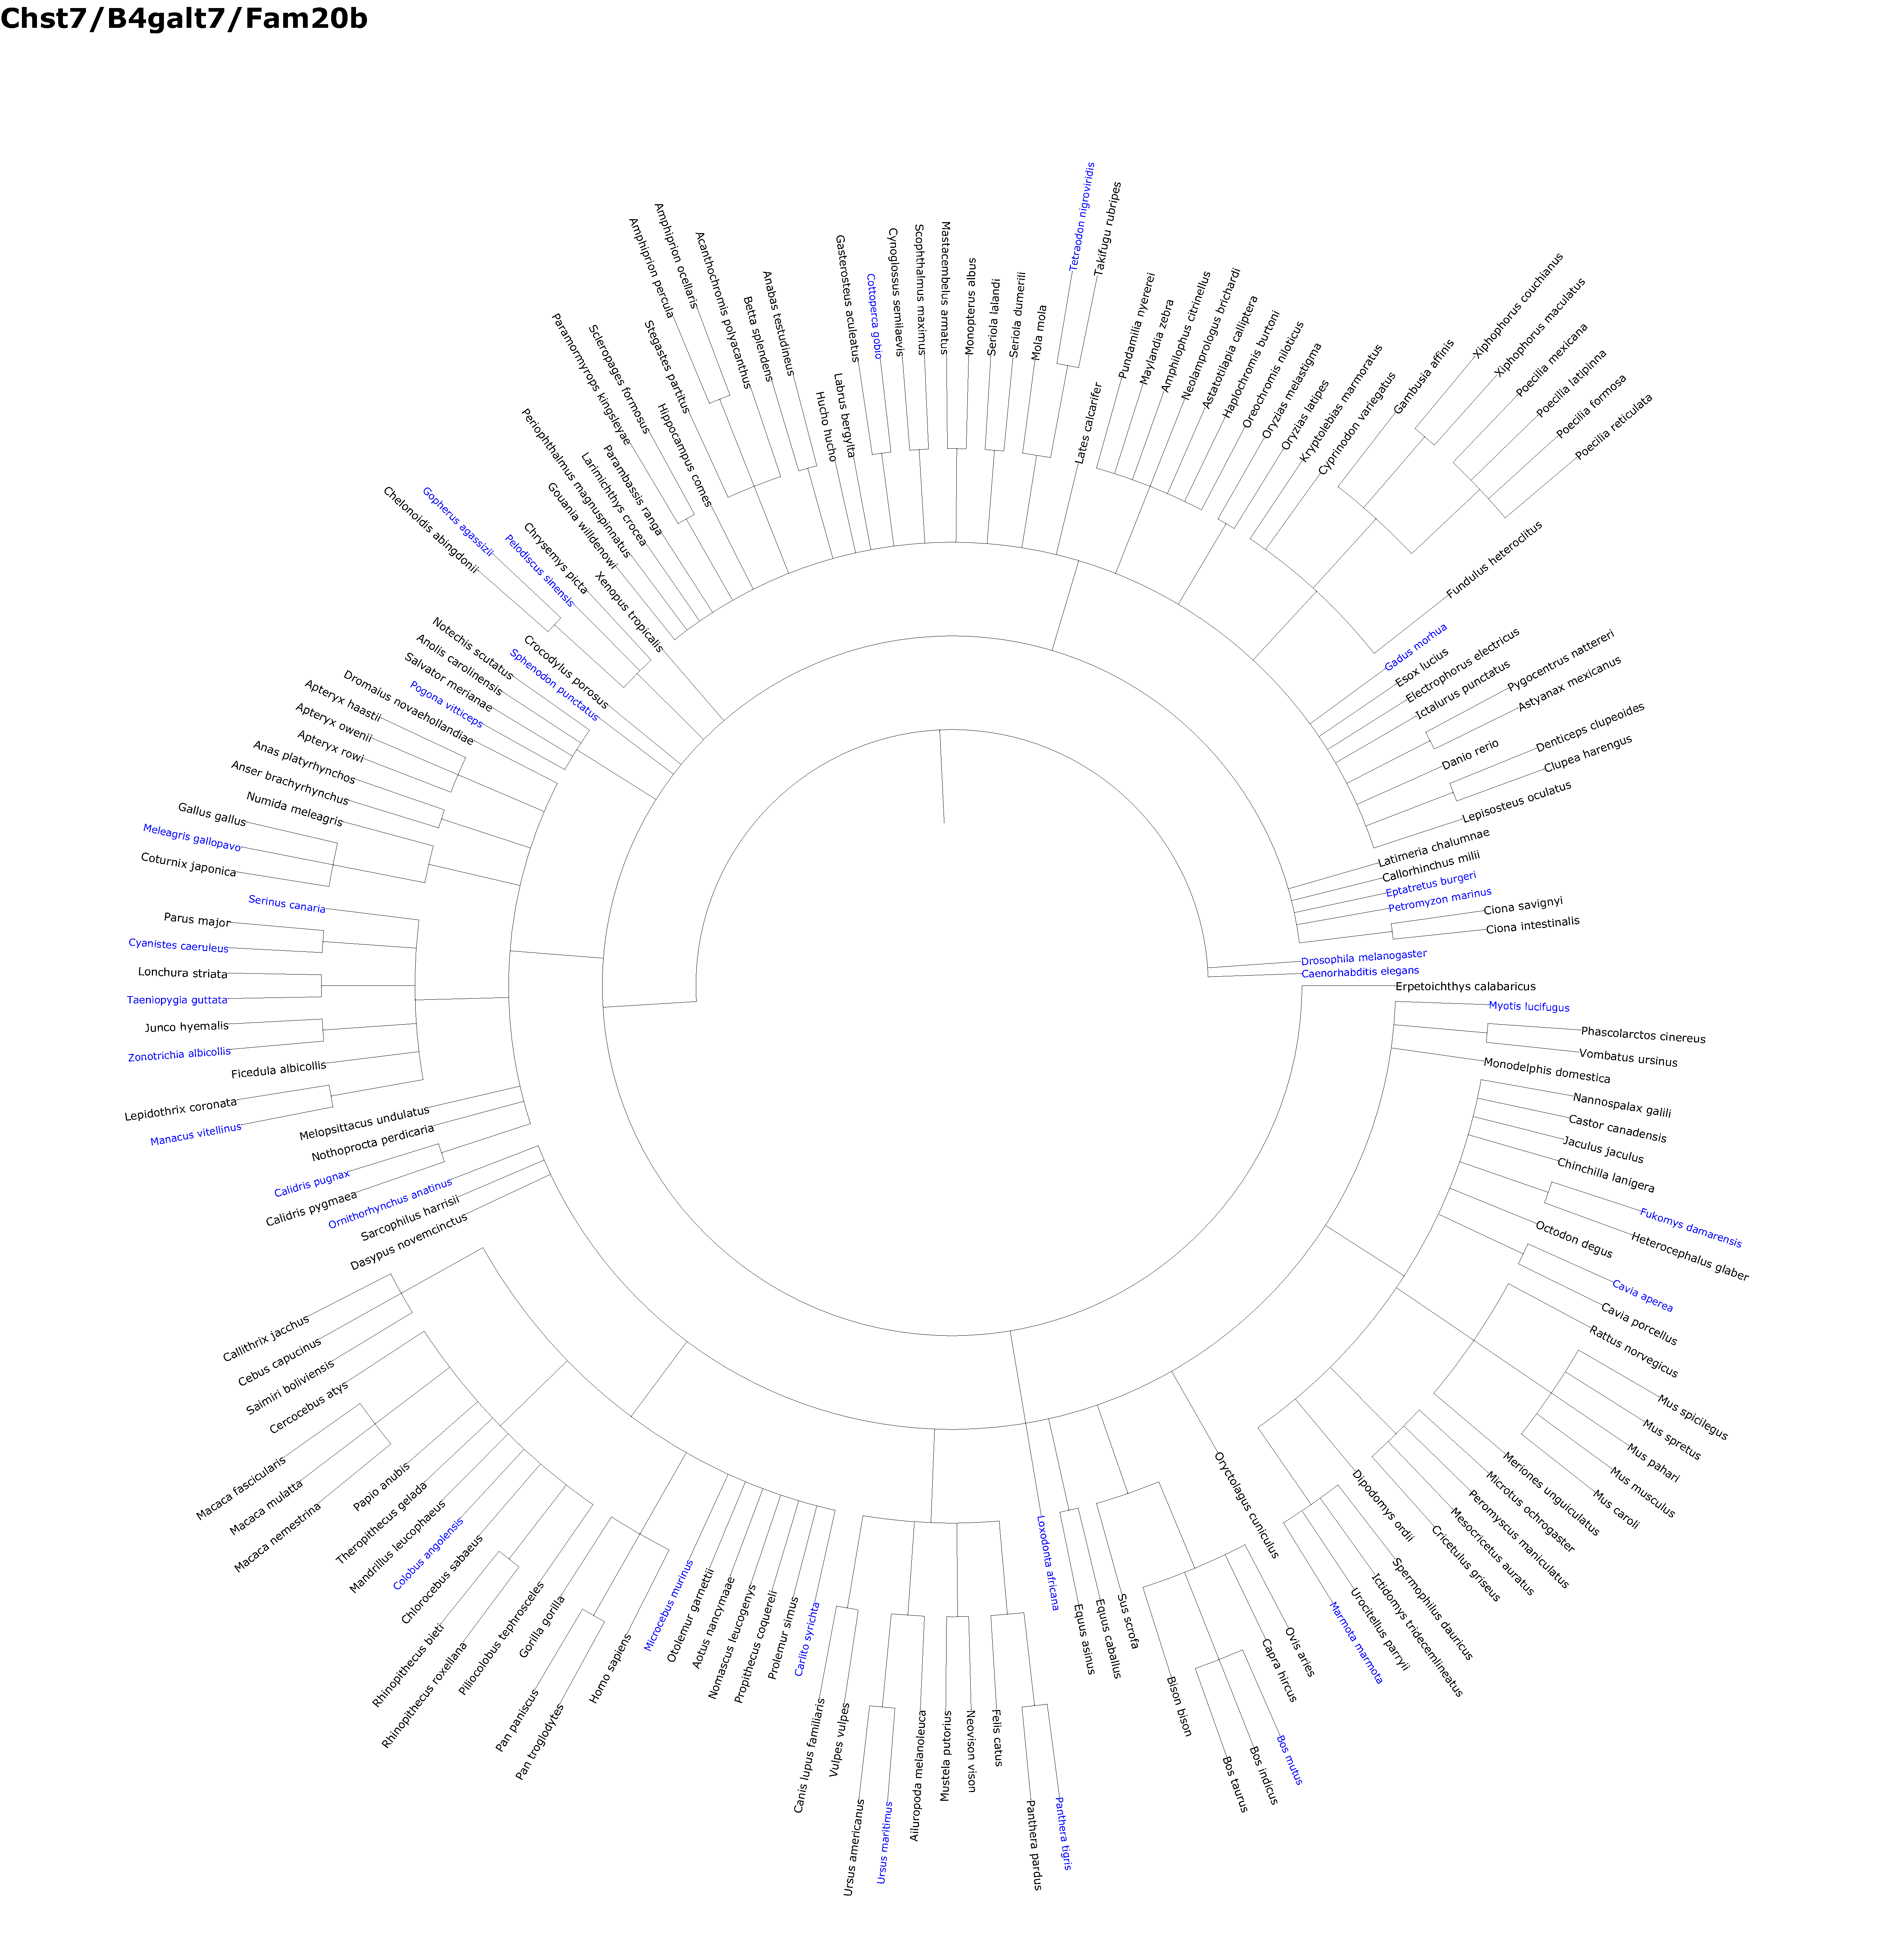
\includegraphics[height=7in,trim={0 0 0 3in},clip]{./appendix_images/trees/Chst7_B4galt7_Fam20b.pdf}}
\caption{\textbf{The gene tree for \textit{Chst7, B4galt7,} and \textit{Fam20b}.}}
\label{sup_fig_11}
\end{figure}

\begin{figure}[H]
\centering
\makebox[\textwidth][c]{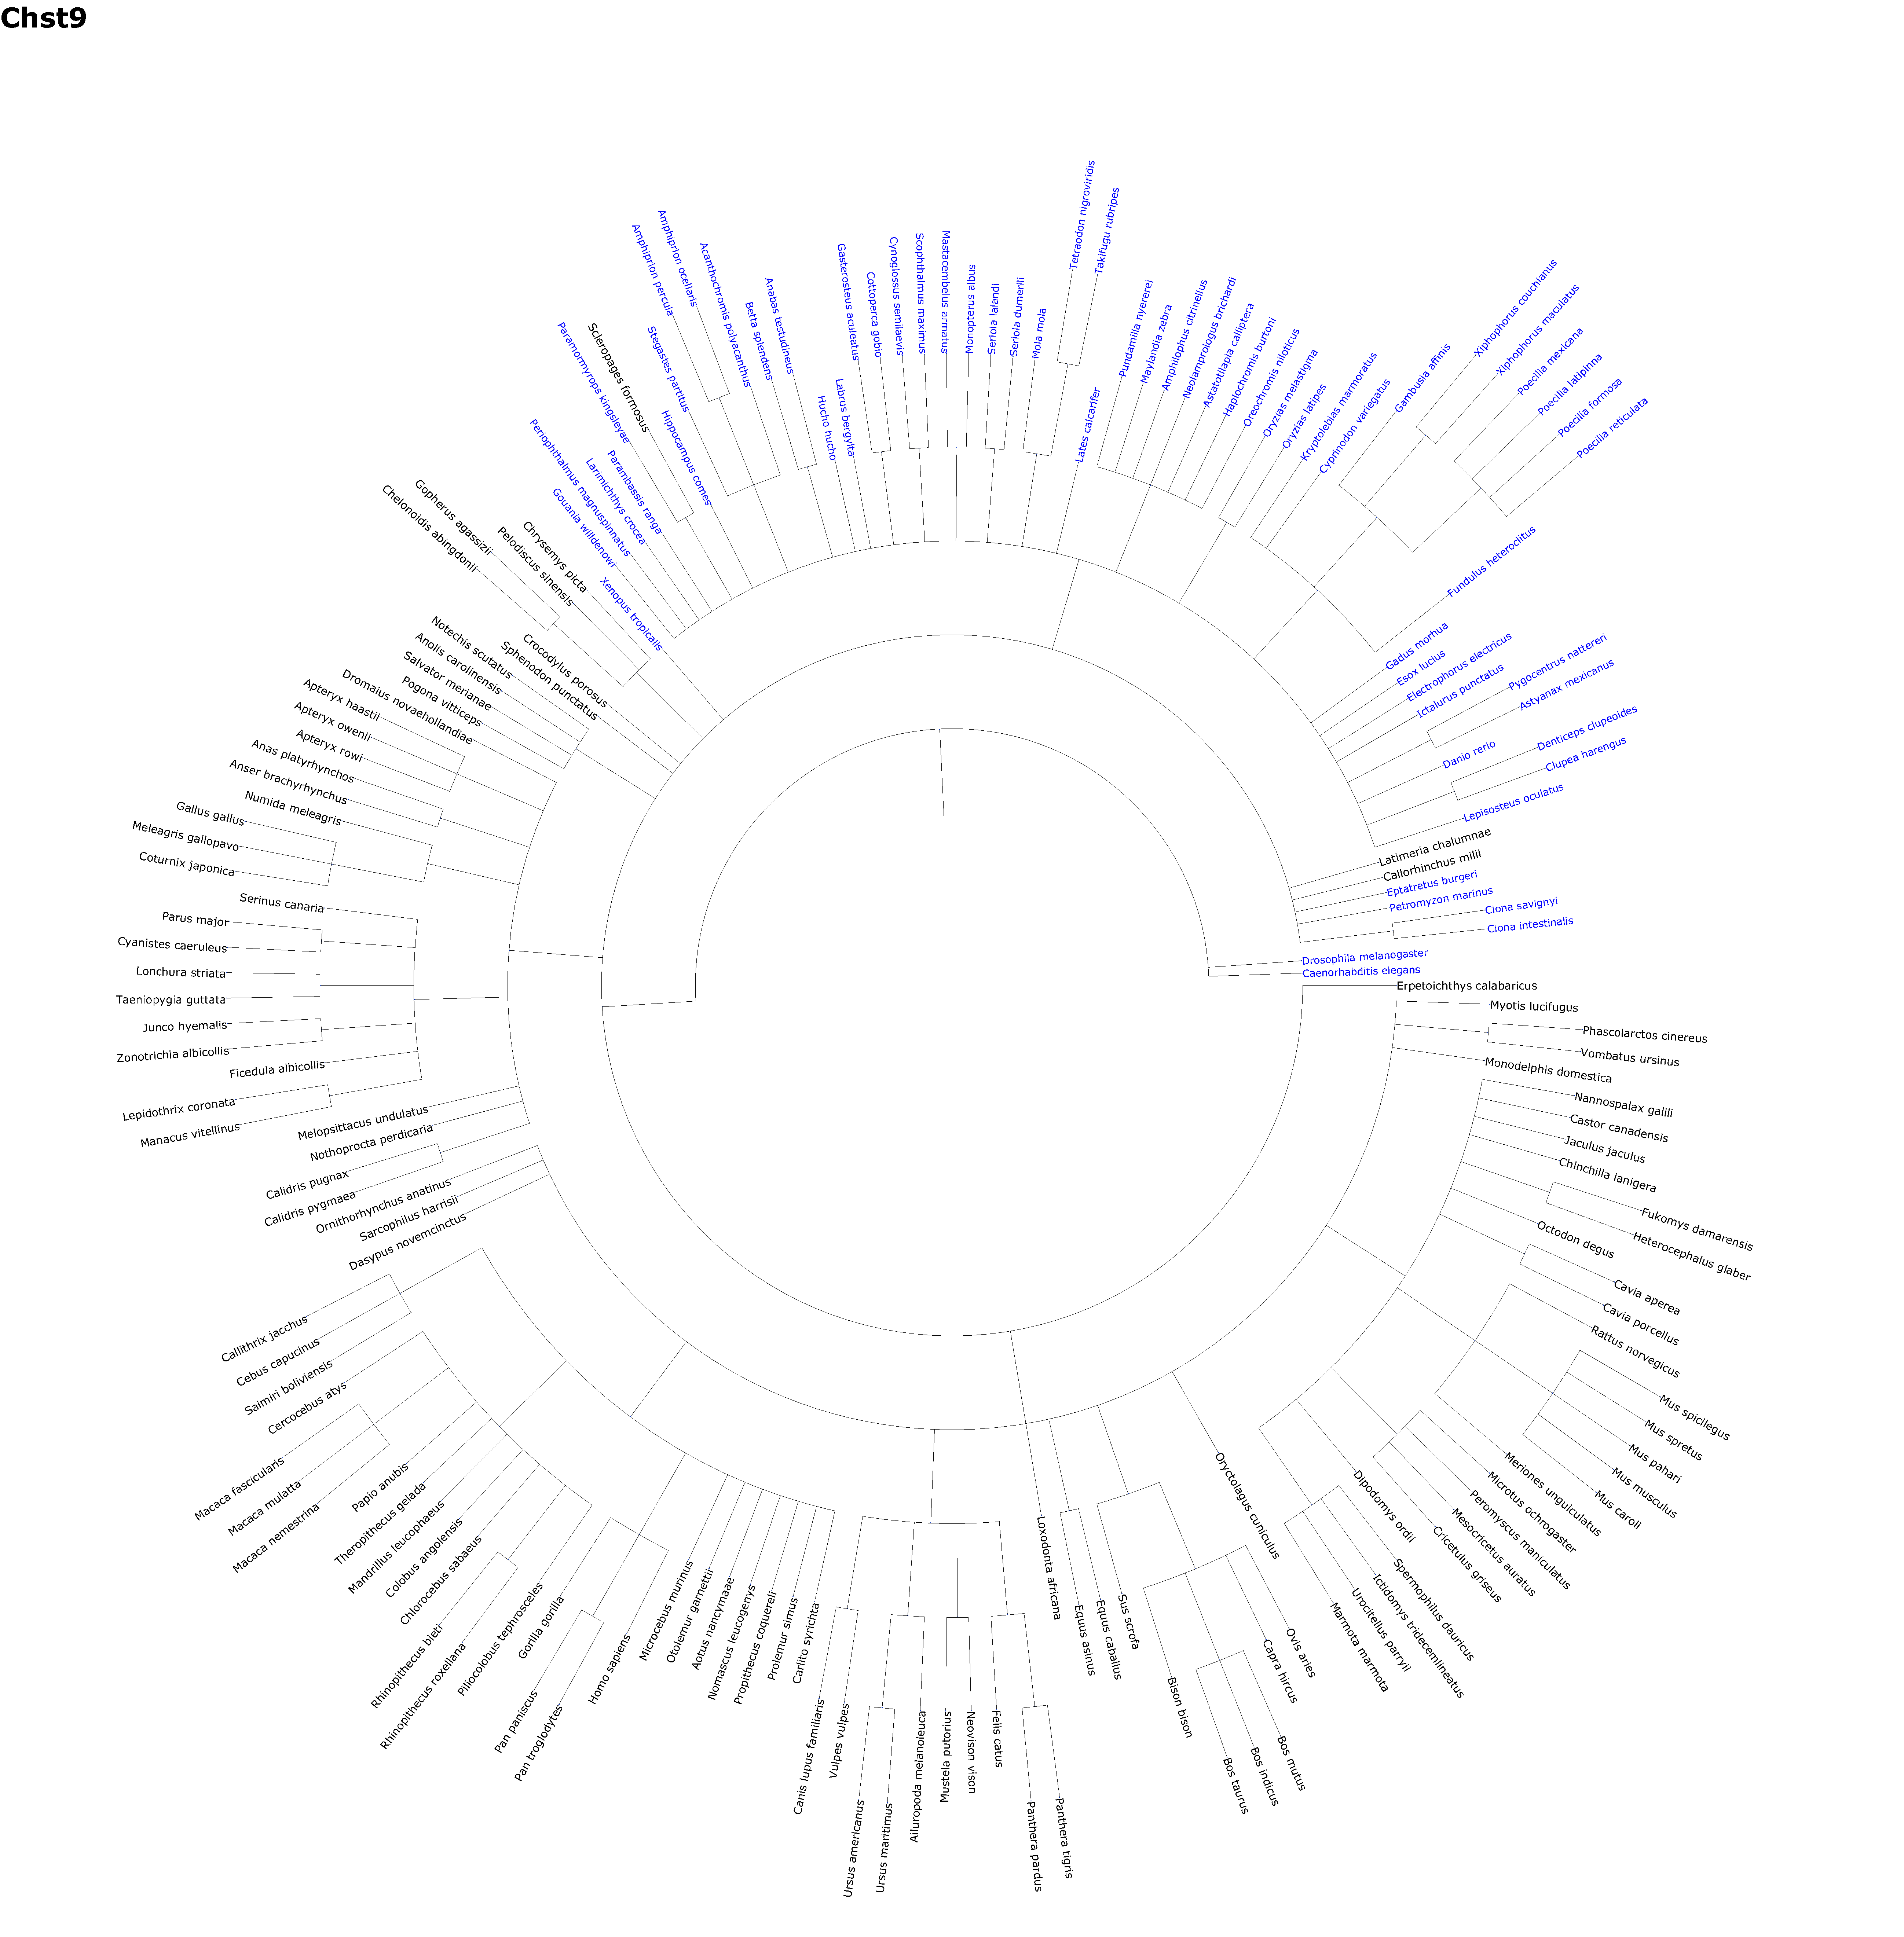
\includegraphics[height=7in,trim={0 0 0 3in},clip]{./appendix_images/trees/Chst9.pdf}}
\caption{\textbf{The gene tree for \textit{Chst9}.}}
\label{sup_fig_12}
\end{figure}

\begin{figure}[H]
\centering
\makebox[\textwidth][c]{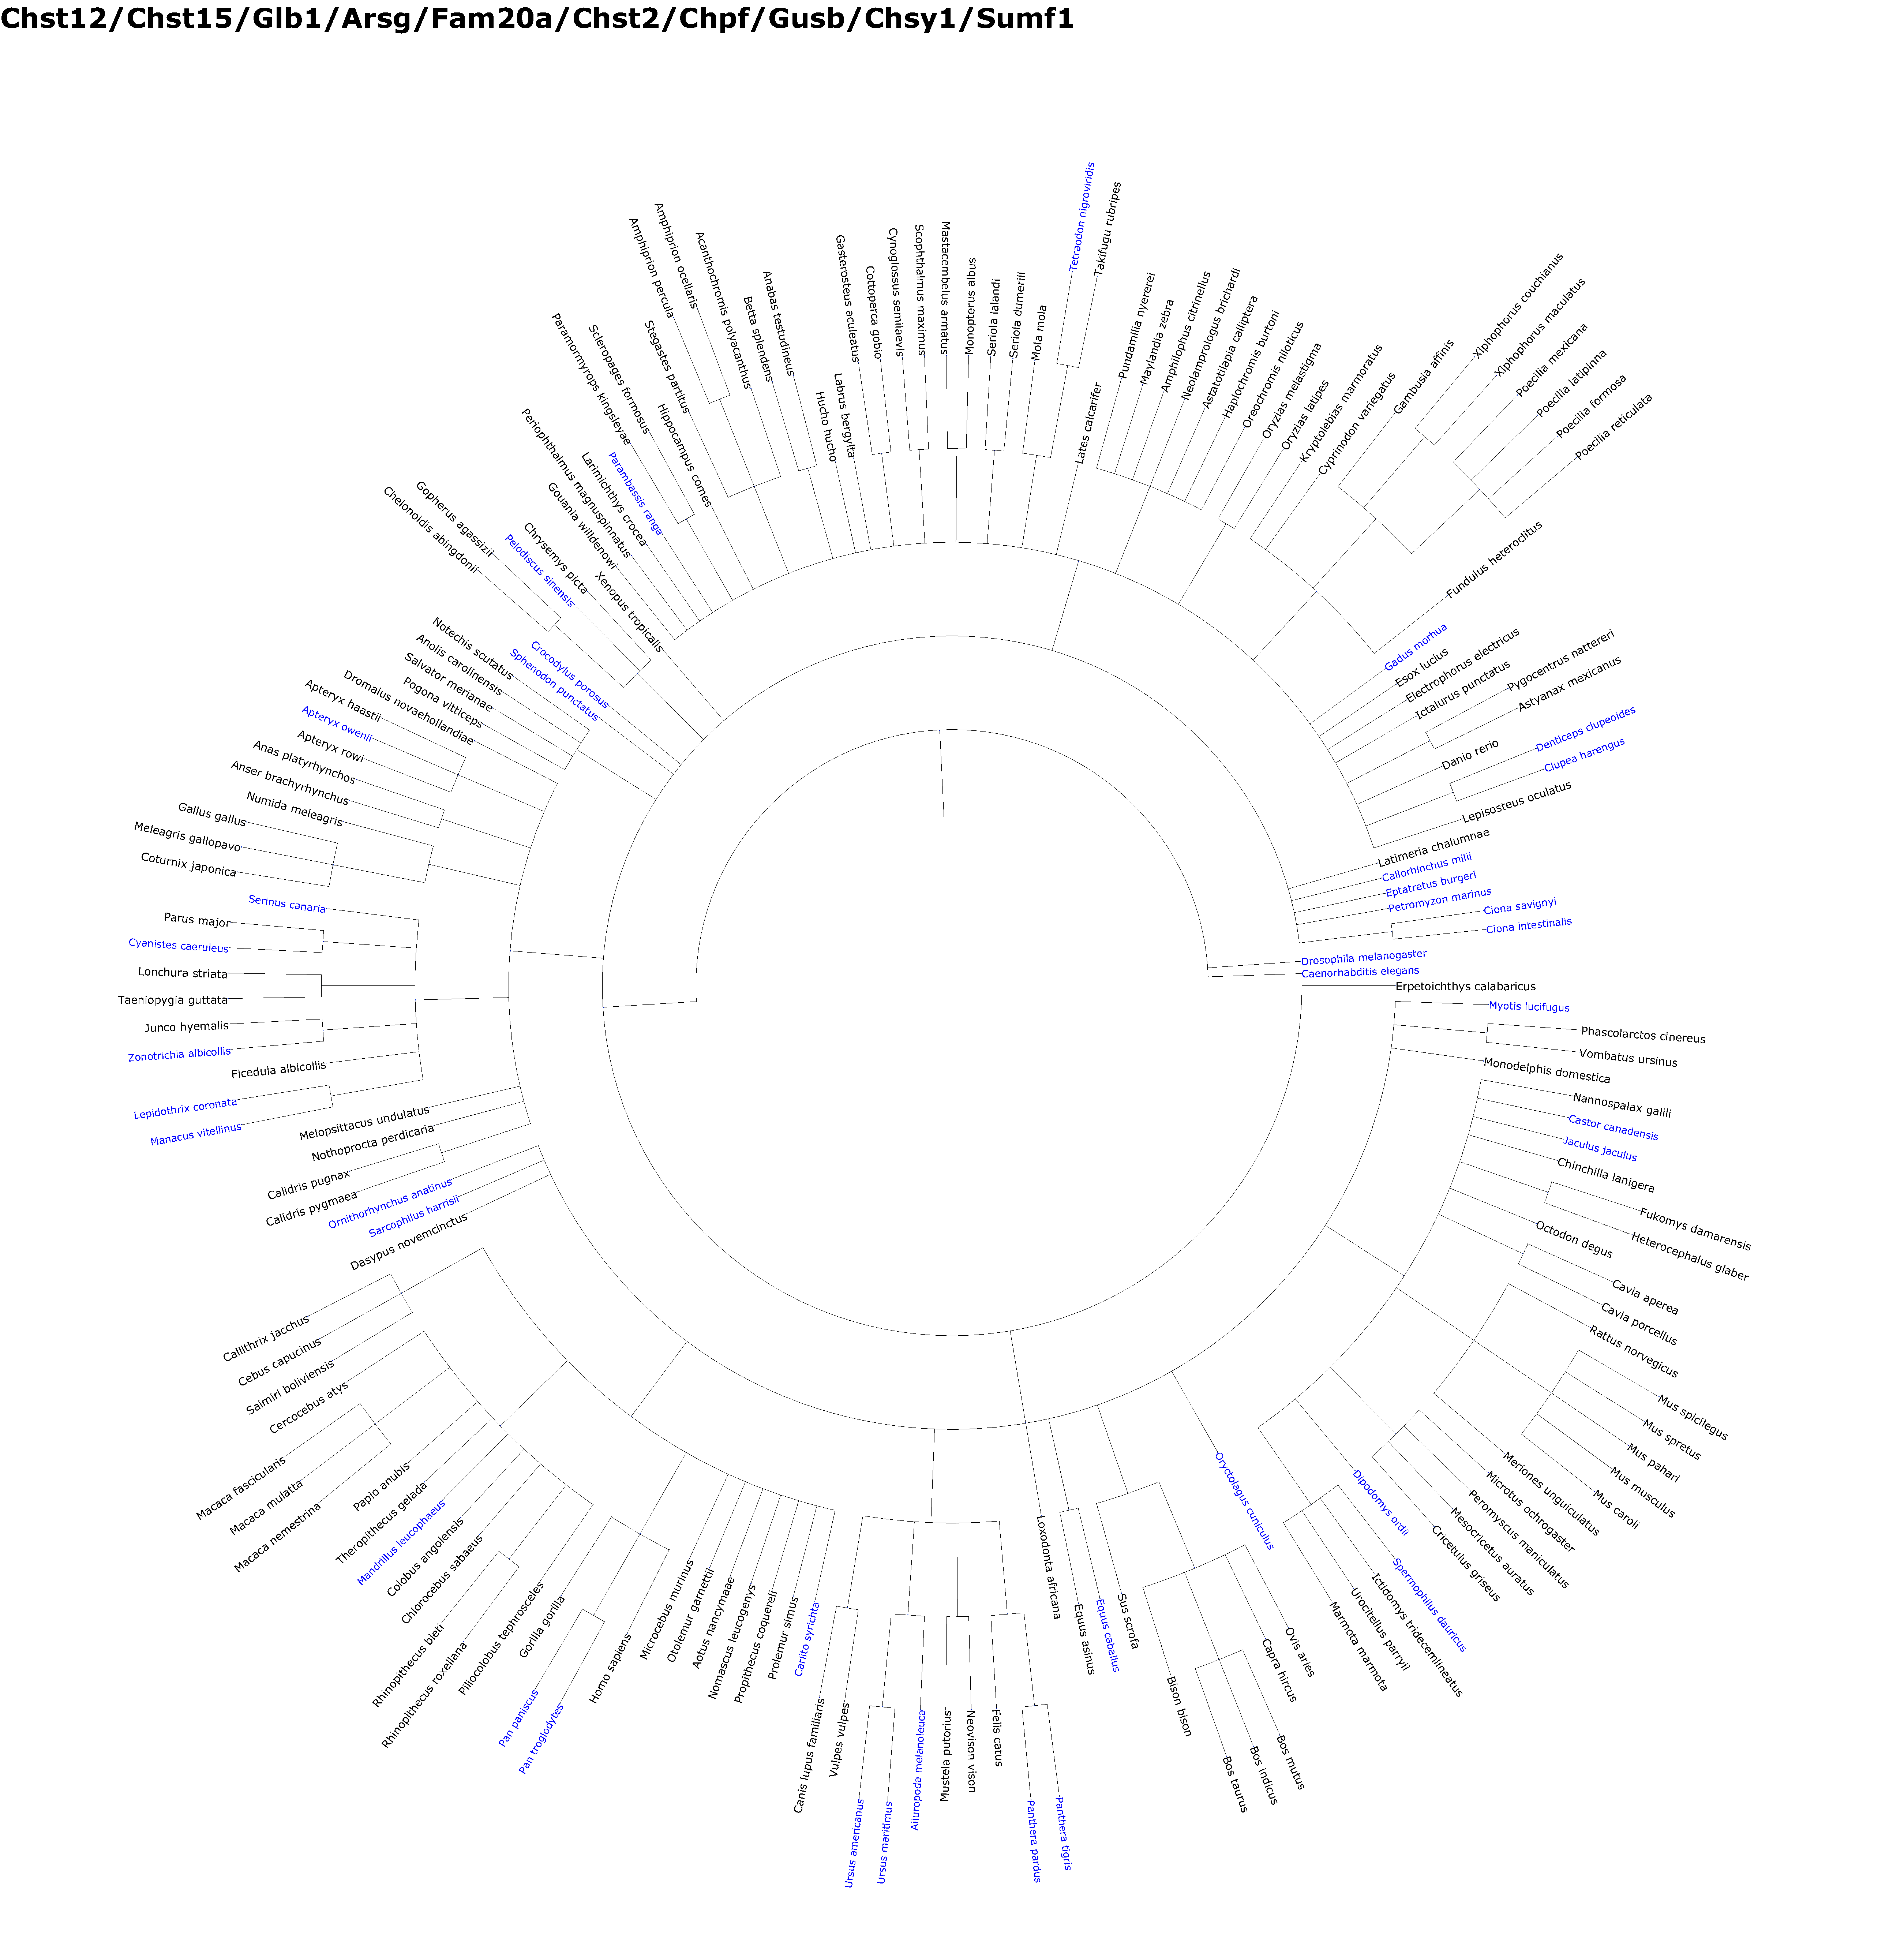
\includegraphics[height=7in,trim={0 0 0 3in},clip]{./appendix_images/trees/Chst12_Chst15_Glb1_Arsg_Fam20a_Chst2_Chpf_Gusb_Chsy1_Sumf1.pdf}}
\caption{\textbf{The gene tree for \textit{Chst12, Chst15, Gib1, Arsg, Fam20a, Chst2, Chpf, Gusb, Chsy1} and \textit{Sumf1}}}
\label{sup_fig_13}
\end{figure}

\begin{figure}[H]
\centering
\makebox[\textwidth][c]{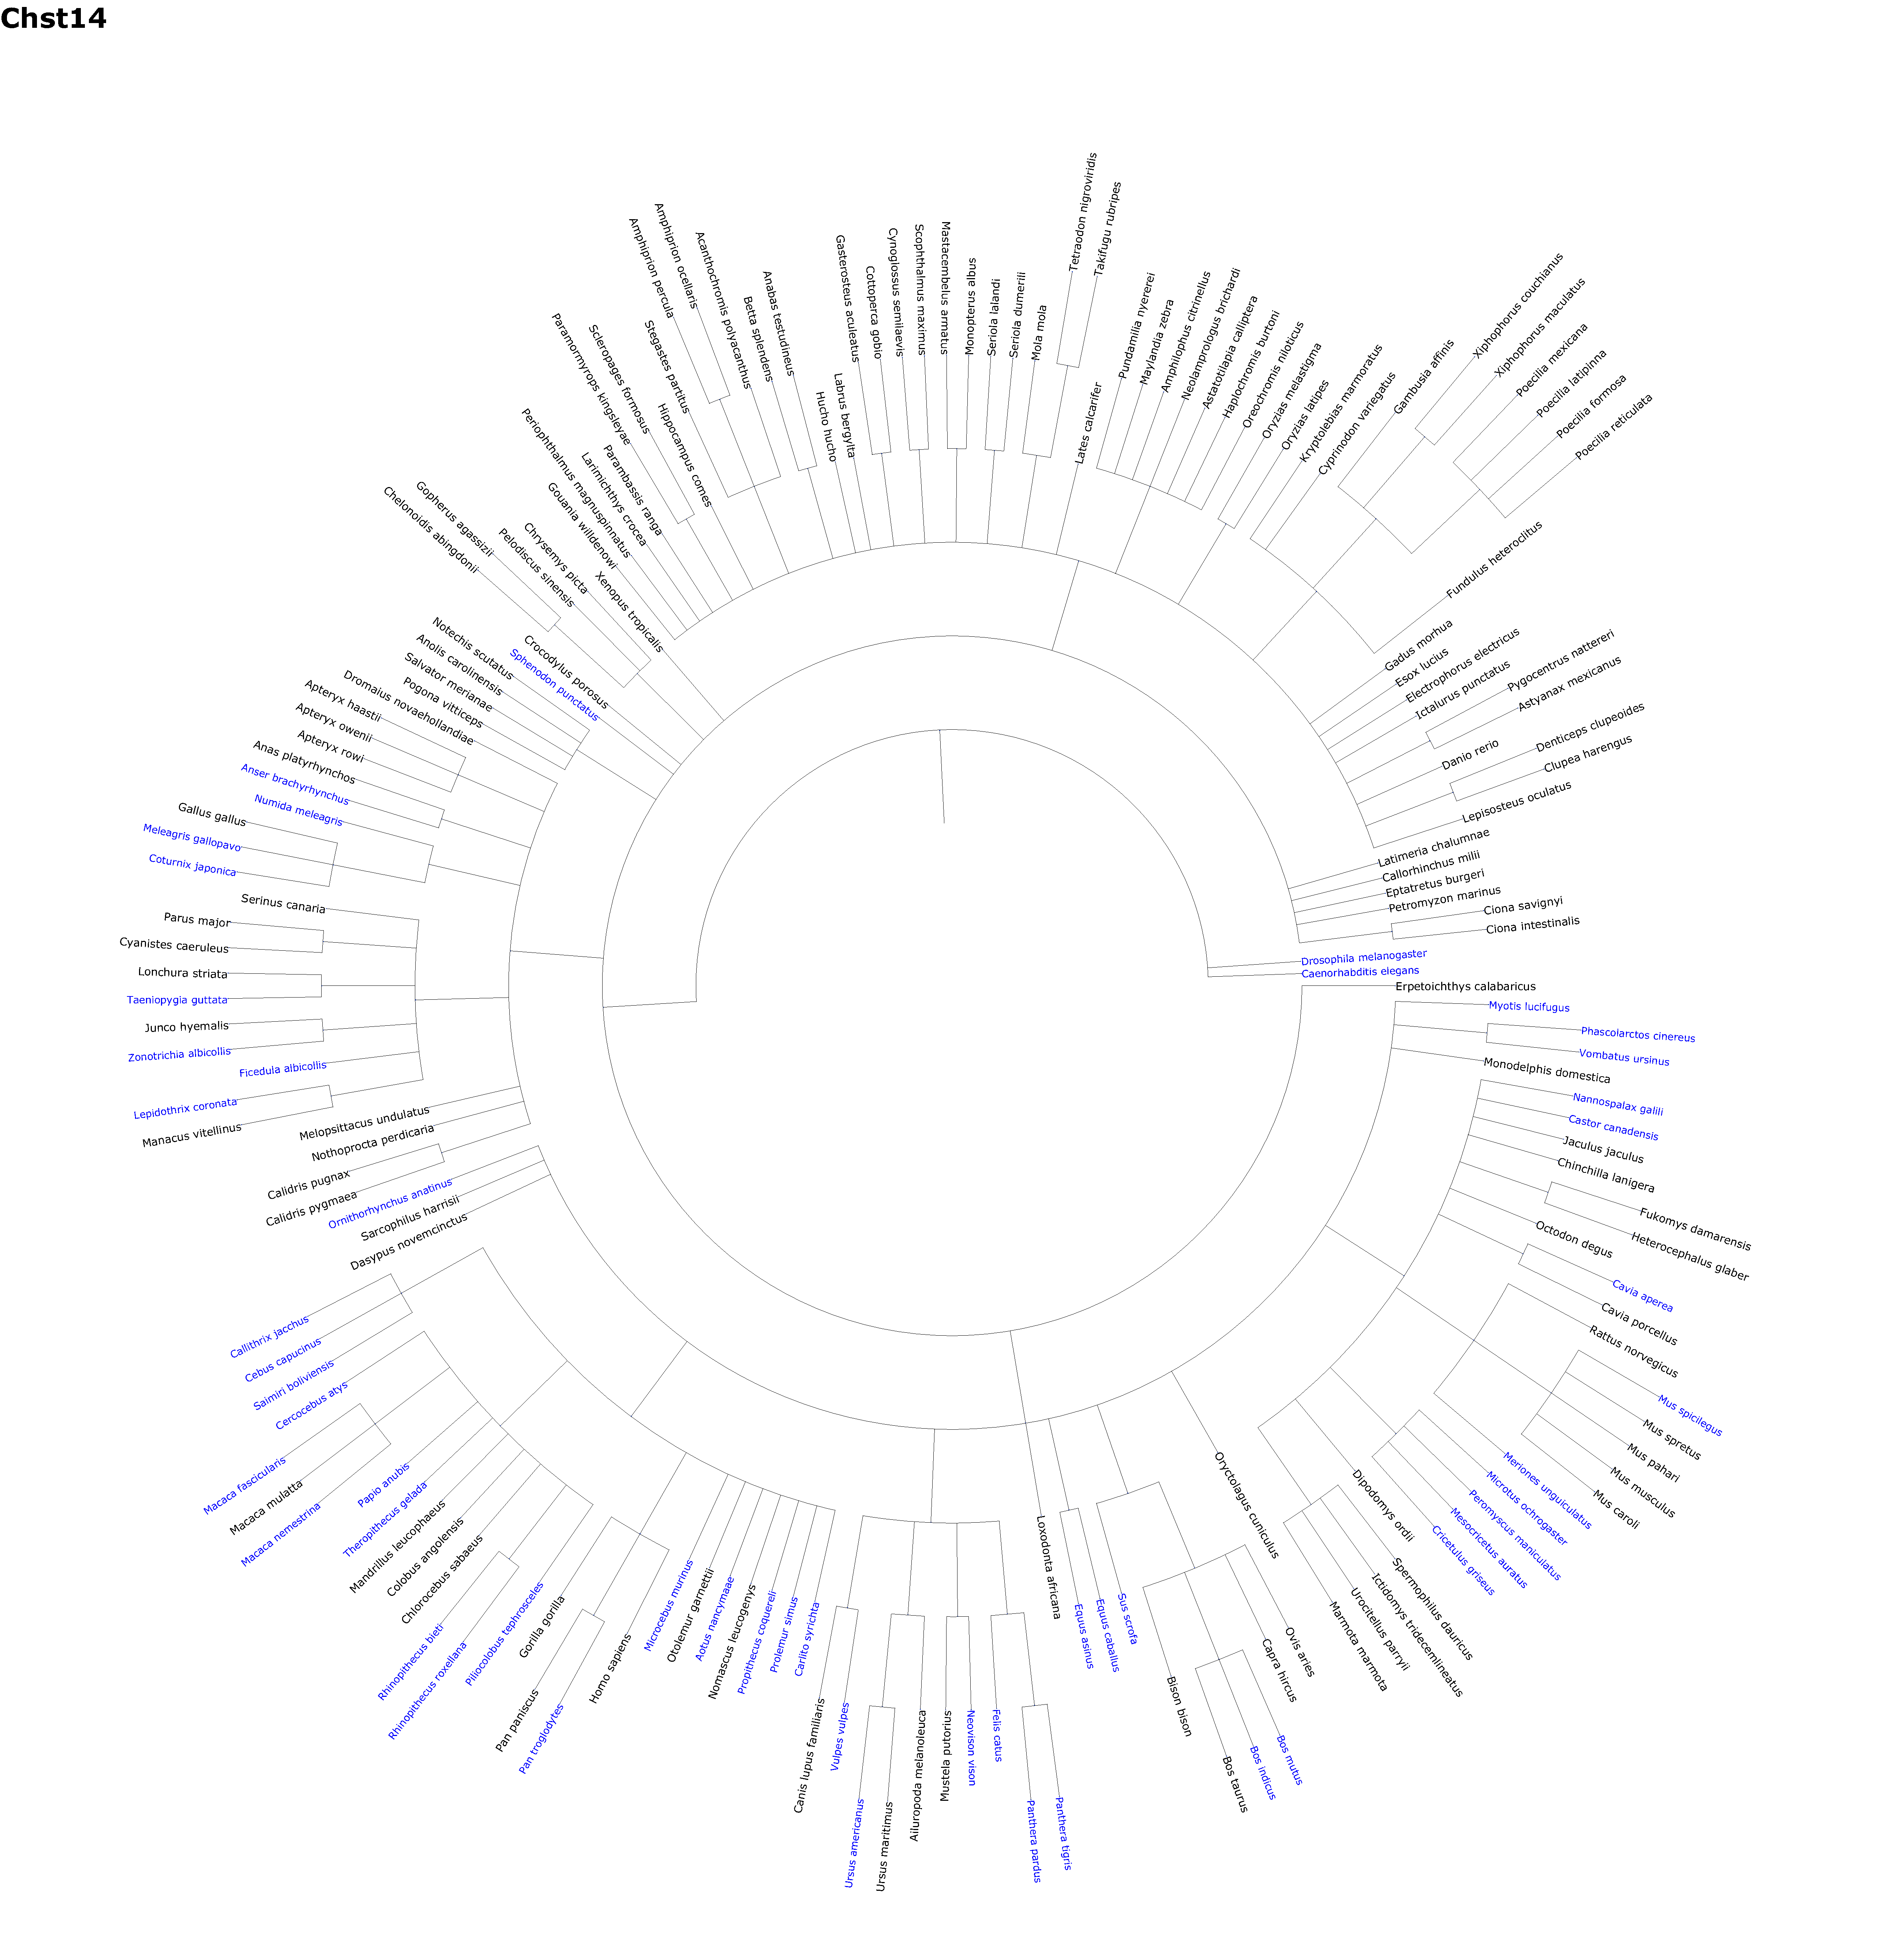
\includegraphics[height=7in,trim={0 0 0 3in},clip]{./appendix_images/trees/Chst14.pdf}}
\caption{\textbf{The gene tree for \textit{Chst14}.}}
\label{sup_fig_14}
\end{figure}

\begin{figure}[H]
\centering
\makebox[\textwidth][c]{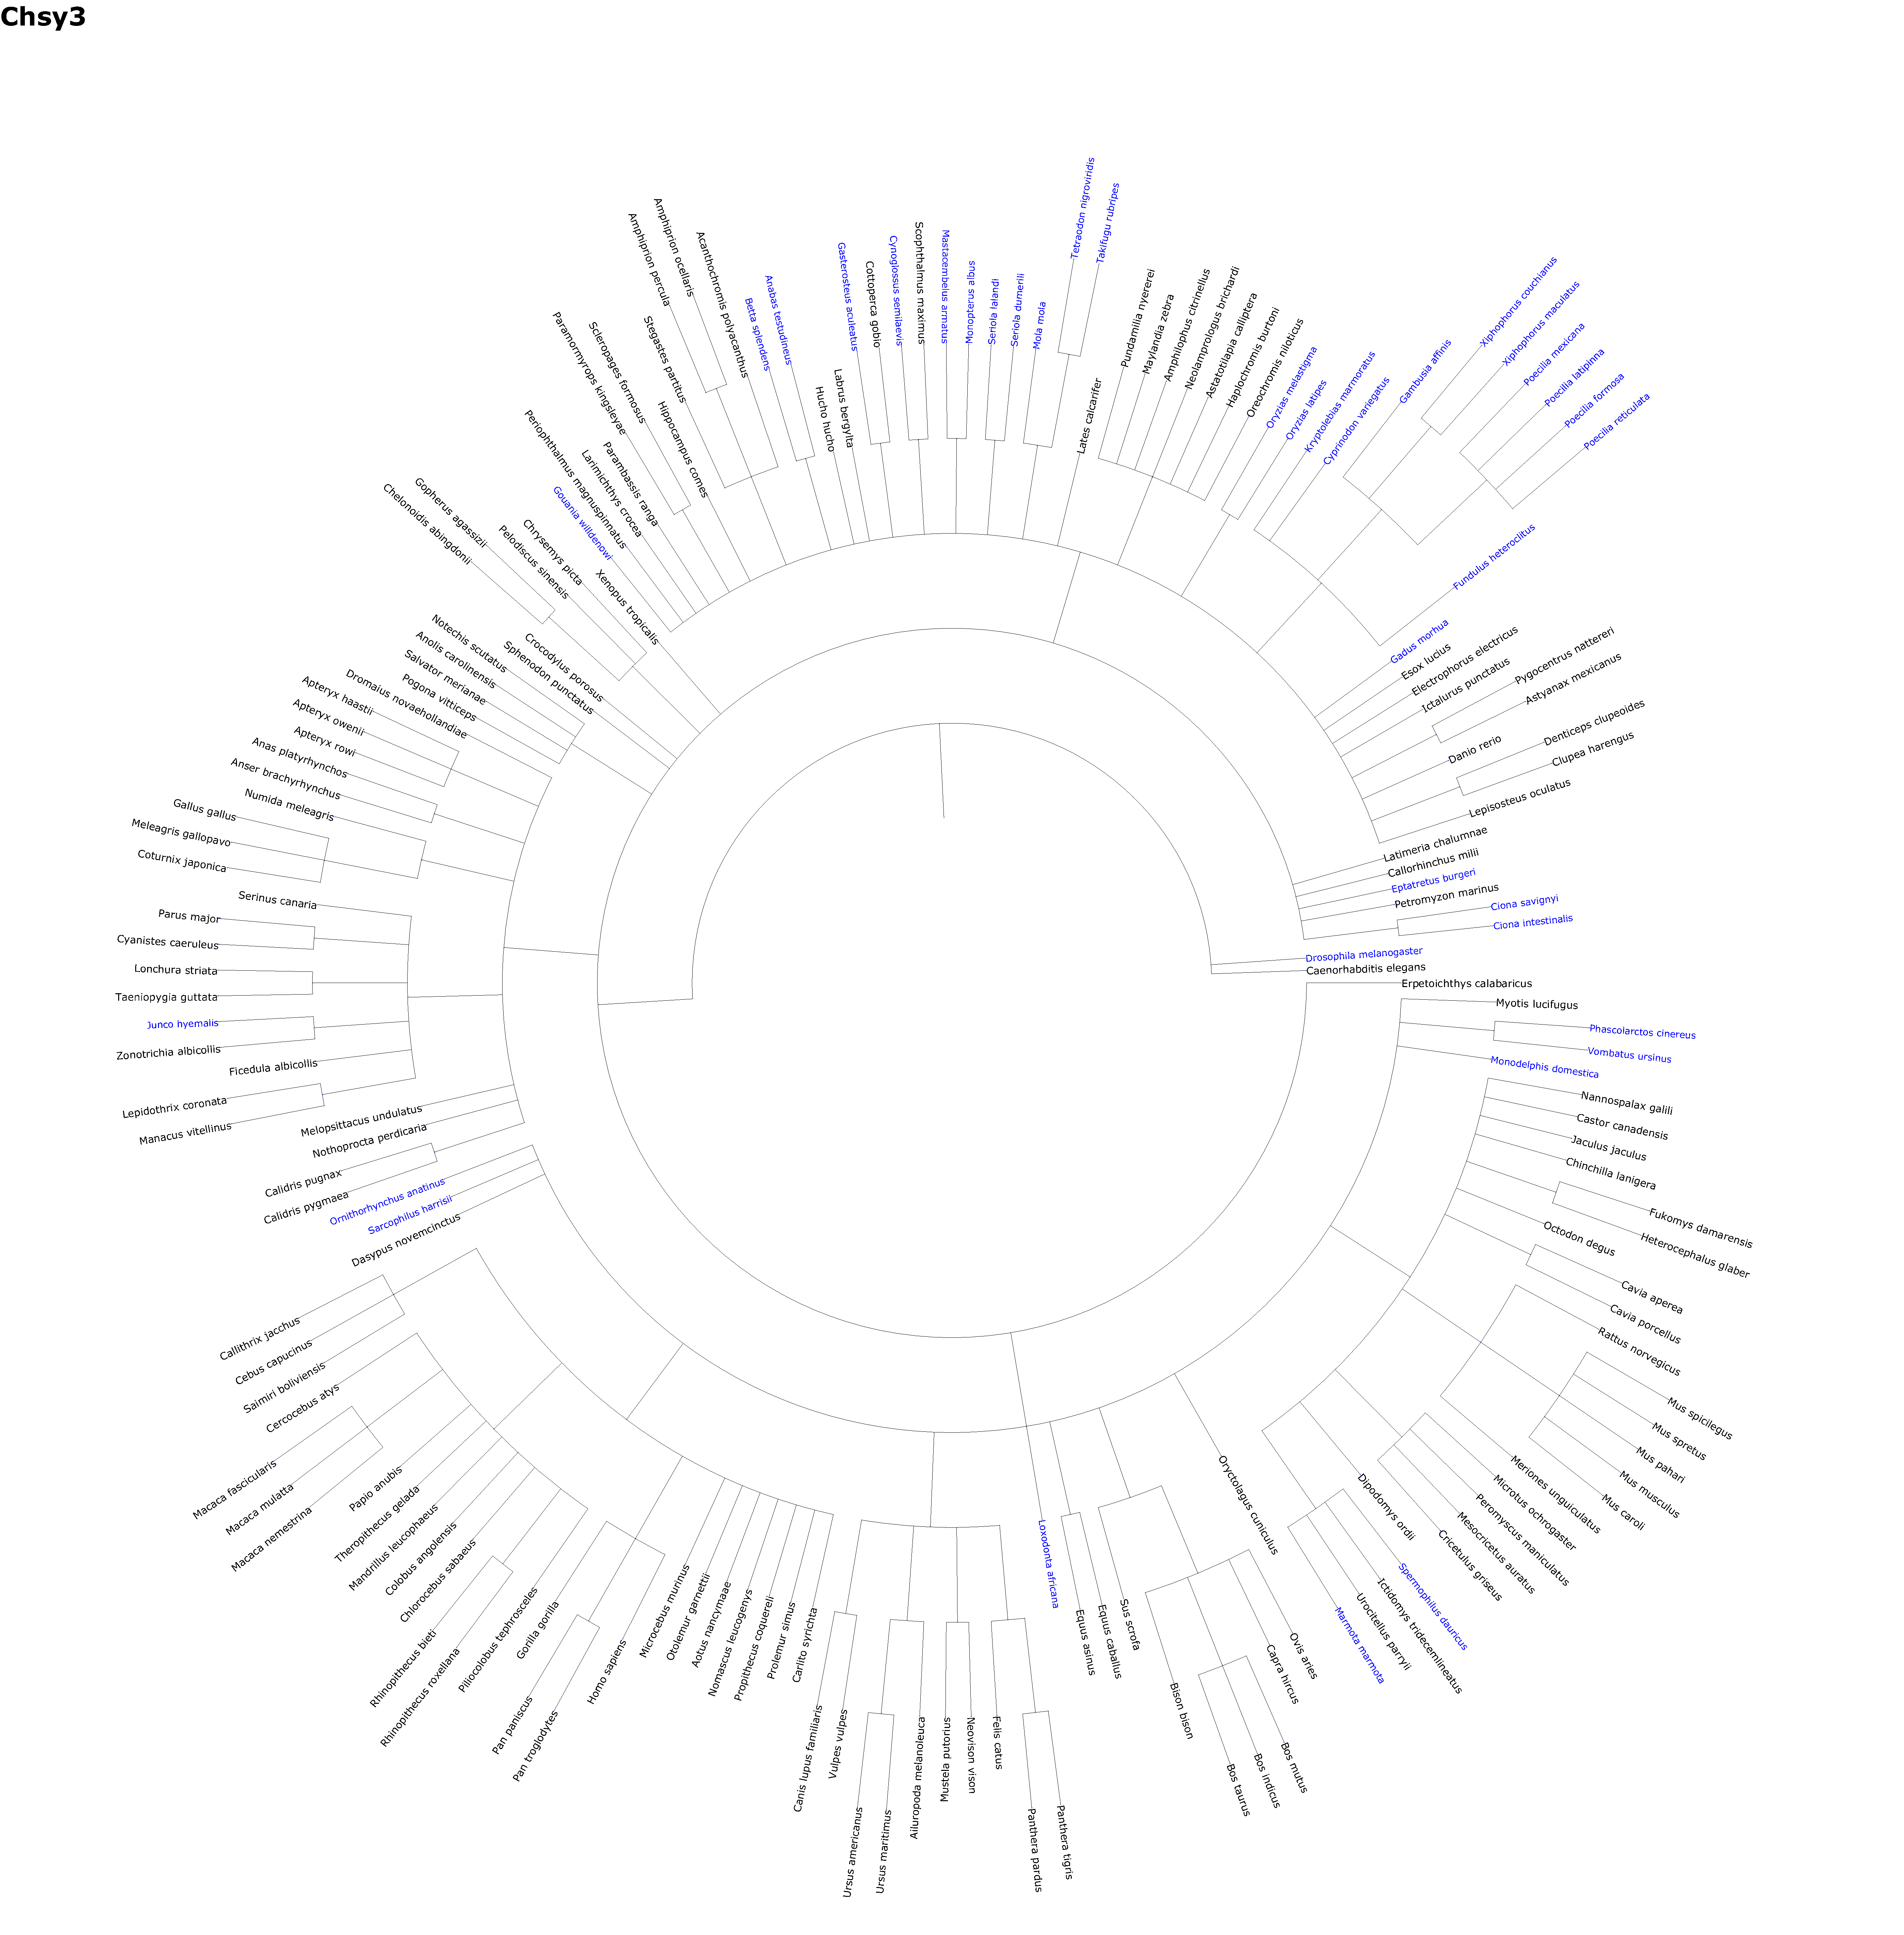
\includegraphics[height=7in,trim={0 0 0 3in},clip]{./appendix_images/trees/Chsy3.pdf}}
\caption{\textbf{The gene tree for \textit{Chsy3}.}}
\label{sup_fig_15}
\end{figure}

\begin{figure}[H]
\centering
\makebox[\textwidth][c]{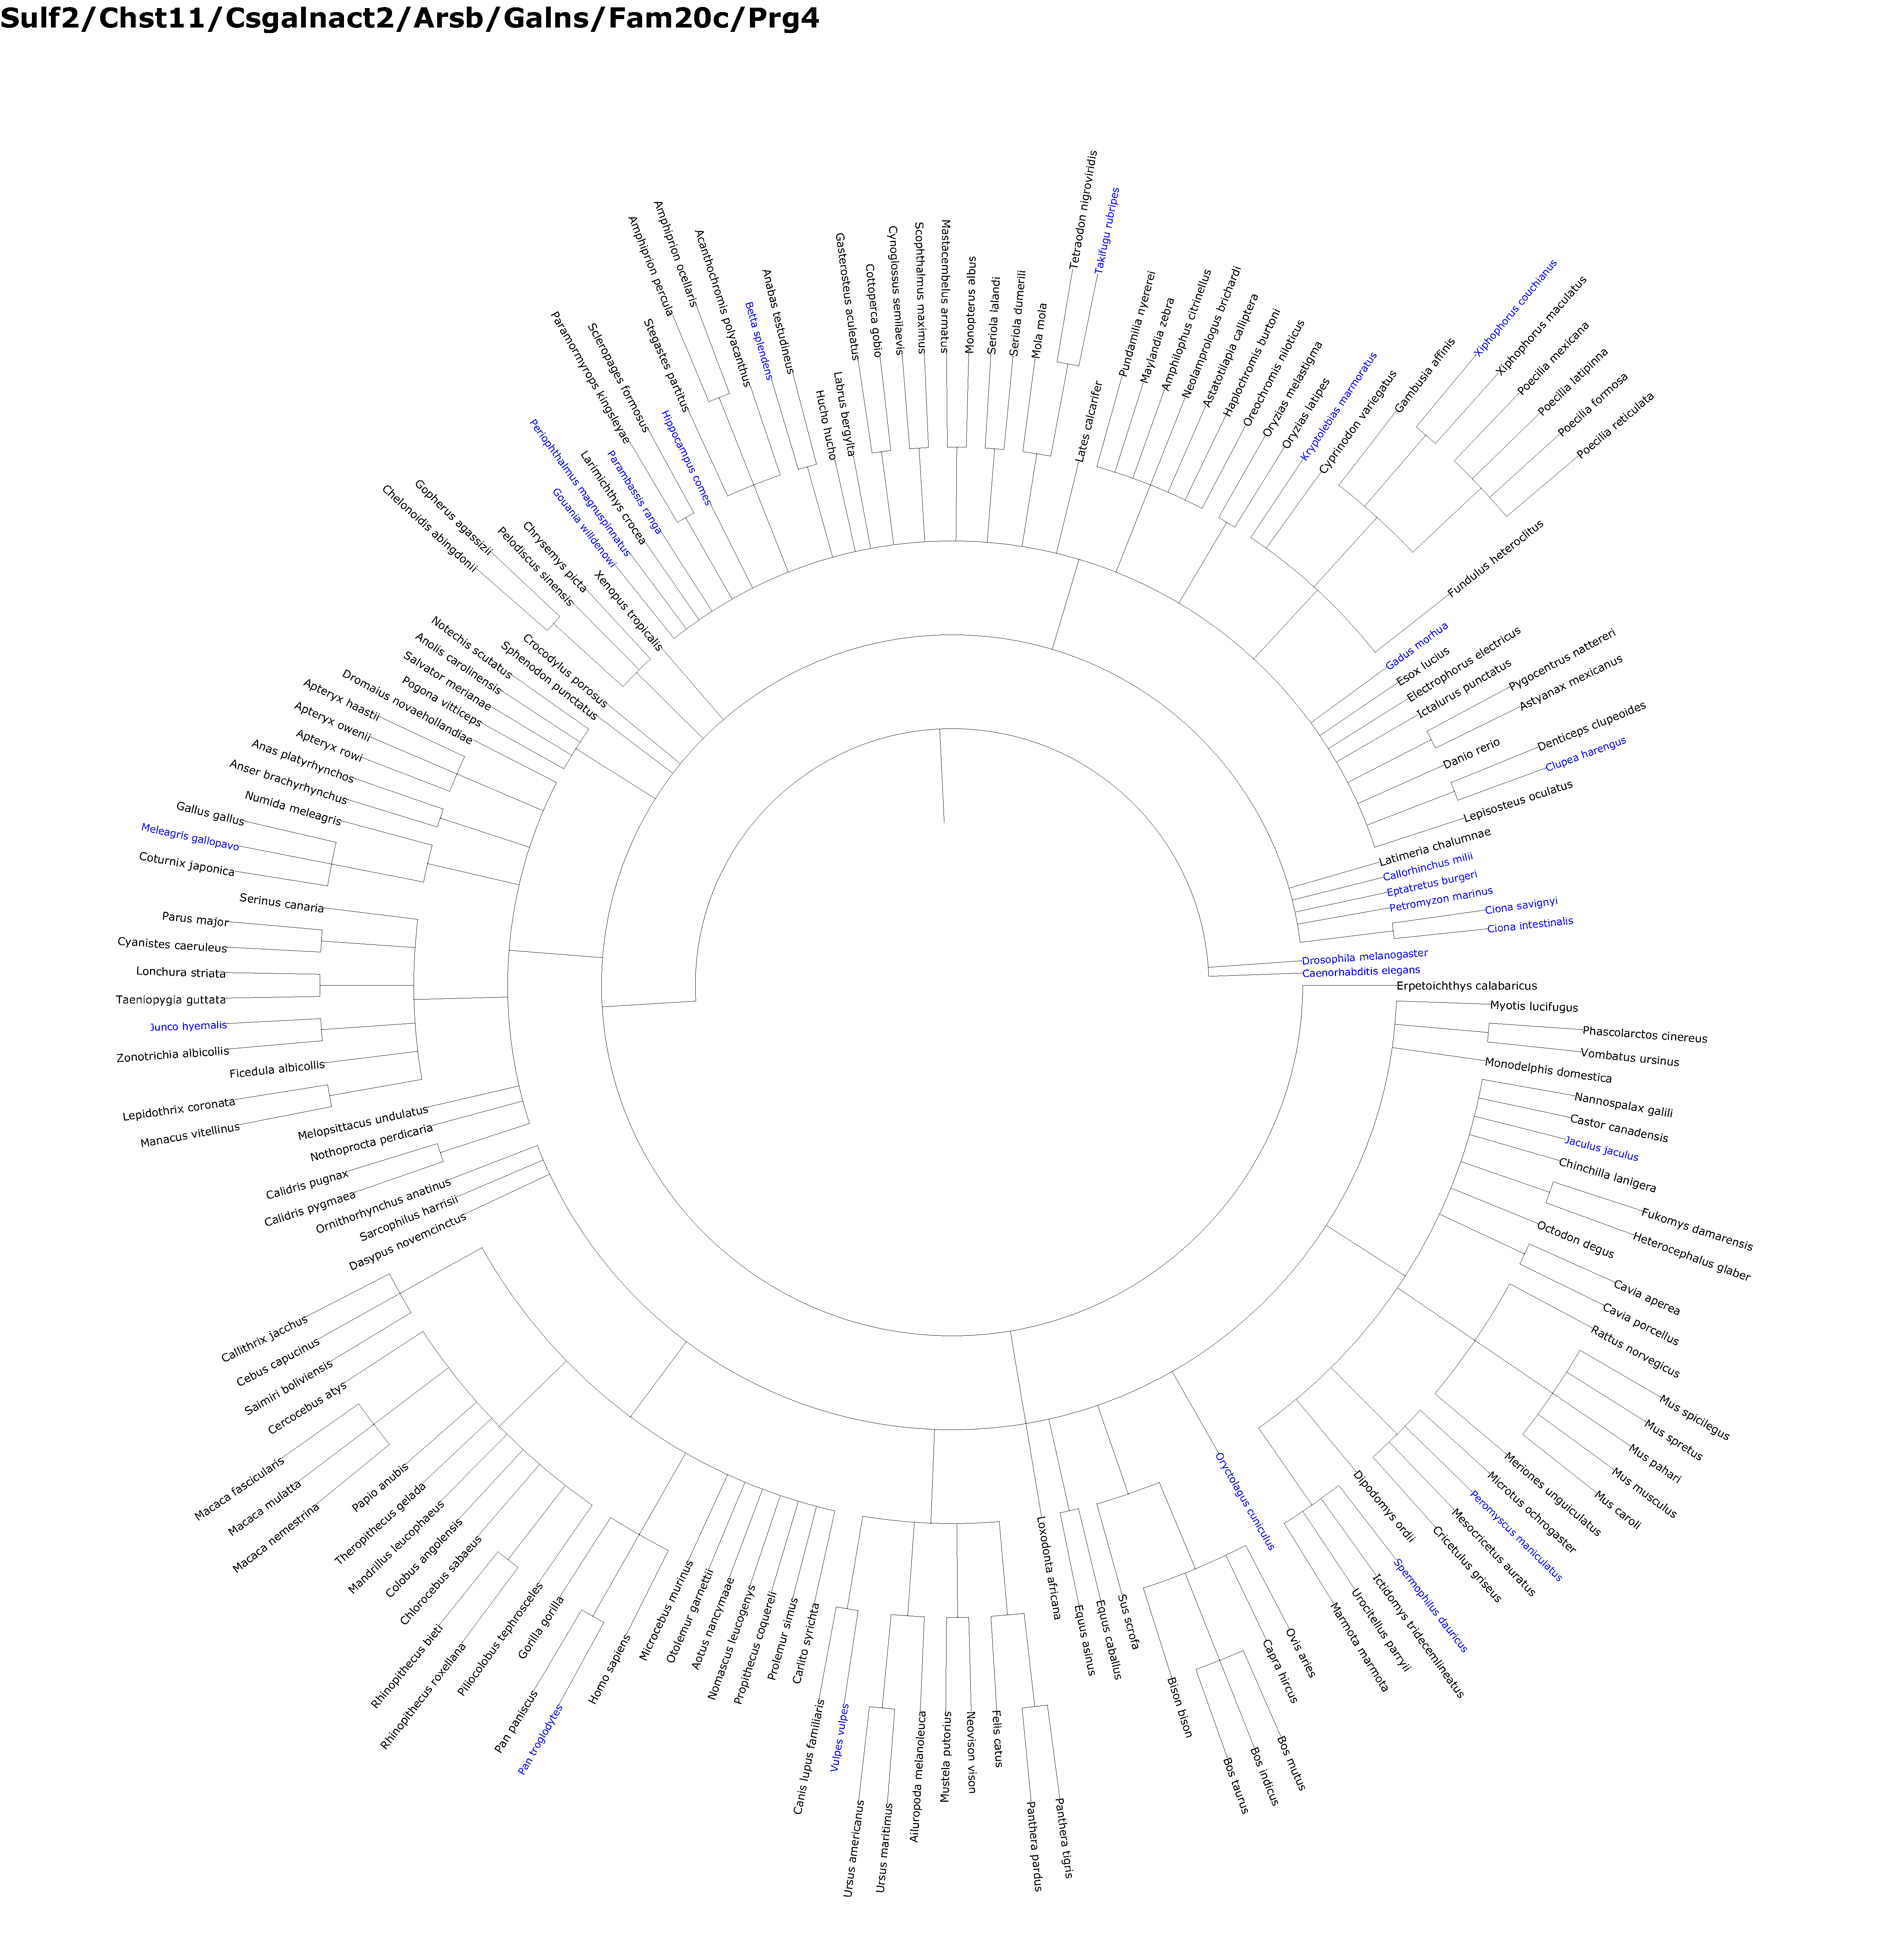
\includegraphics[height=7in,trim={0 0 0 3in},clip]{./appendix_images/trees/Sulf2_Chst11_Csgalnact2_Arsb_Galns_Fam20c_Prg4.pdf}}
\caption{\textbf{The gene tree for \textit{Sulf2, Chst11, Csgalnact2, Arsb, Galns, Fam20c}, and \textit{Prg4}.}}
\label{sup_fig_16}
\end{figure}

\begin{figure}[H]
\centering
\makebox[\textwidth][c]{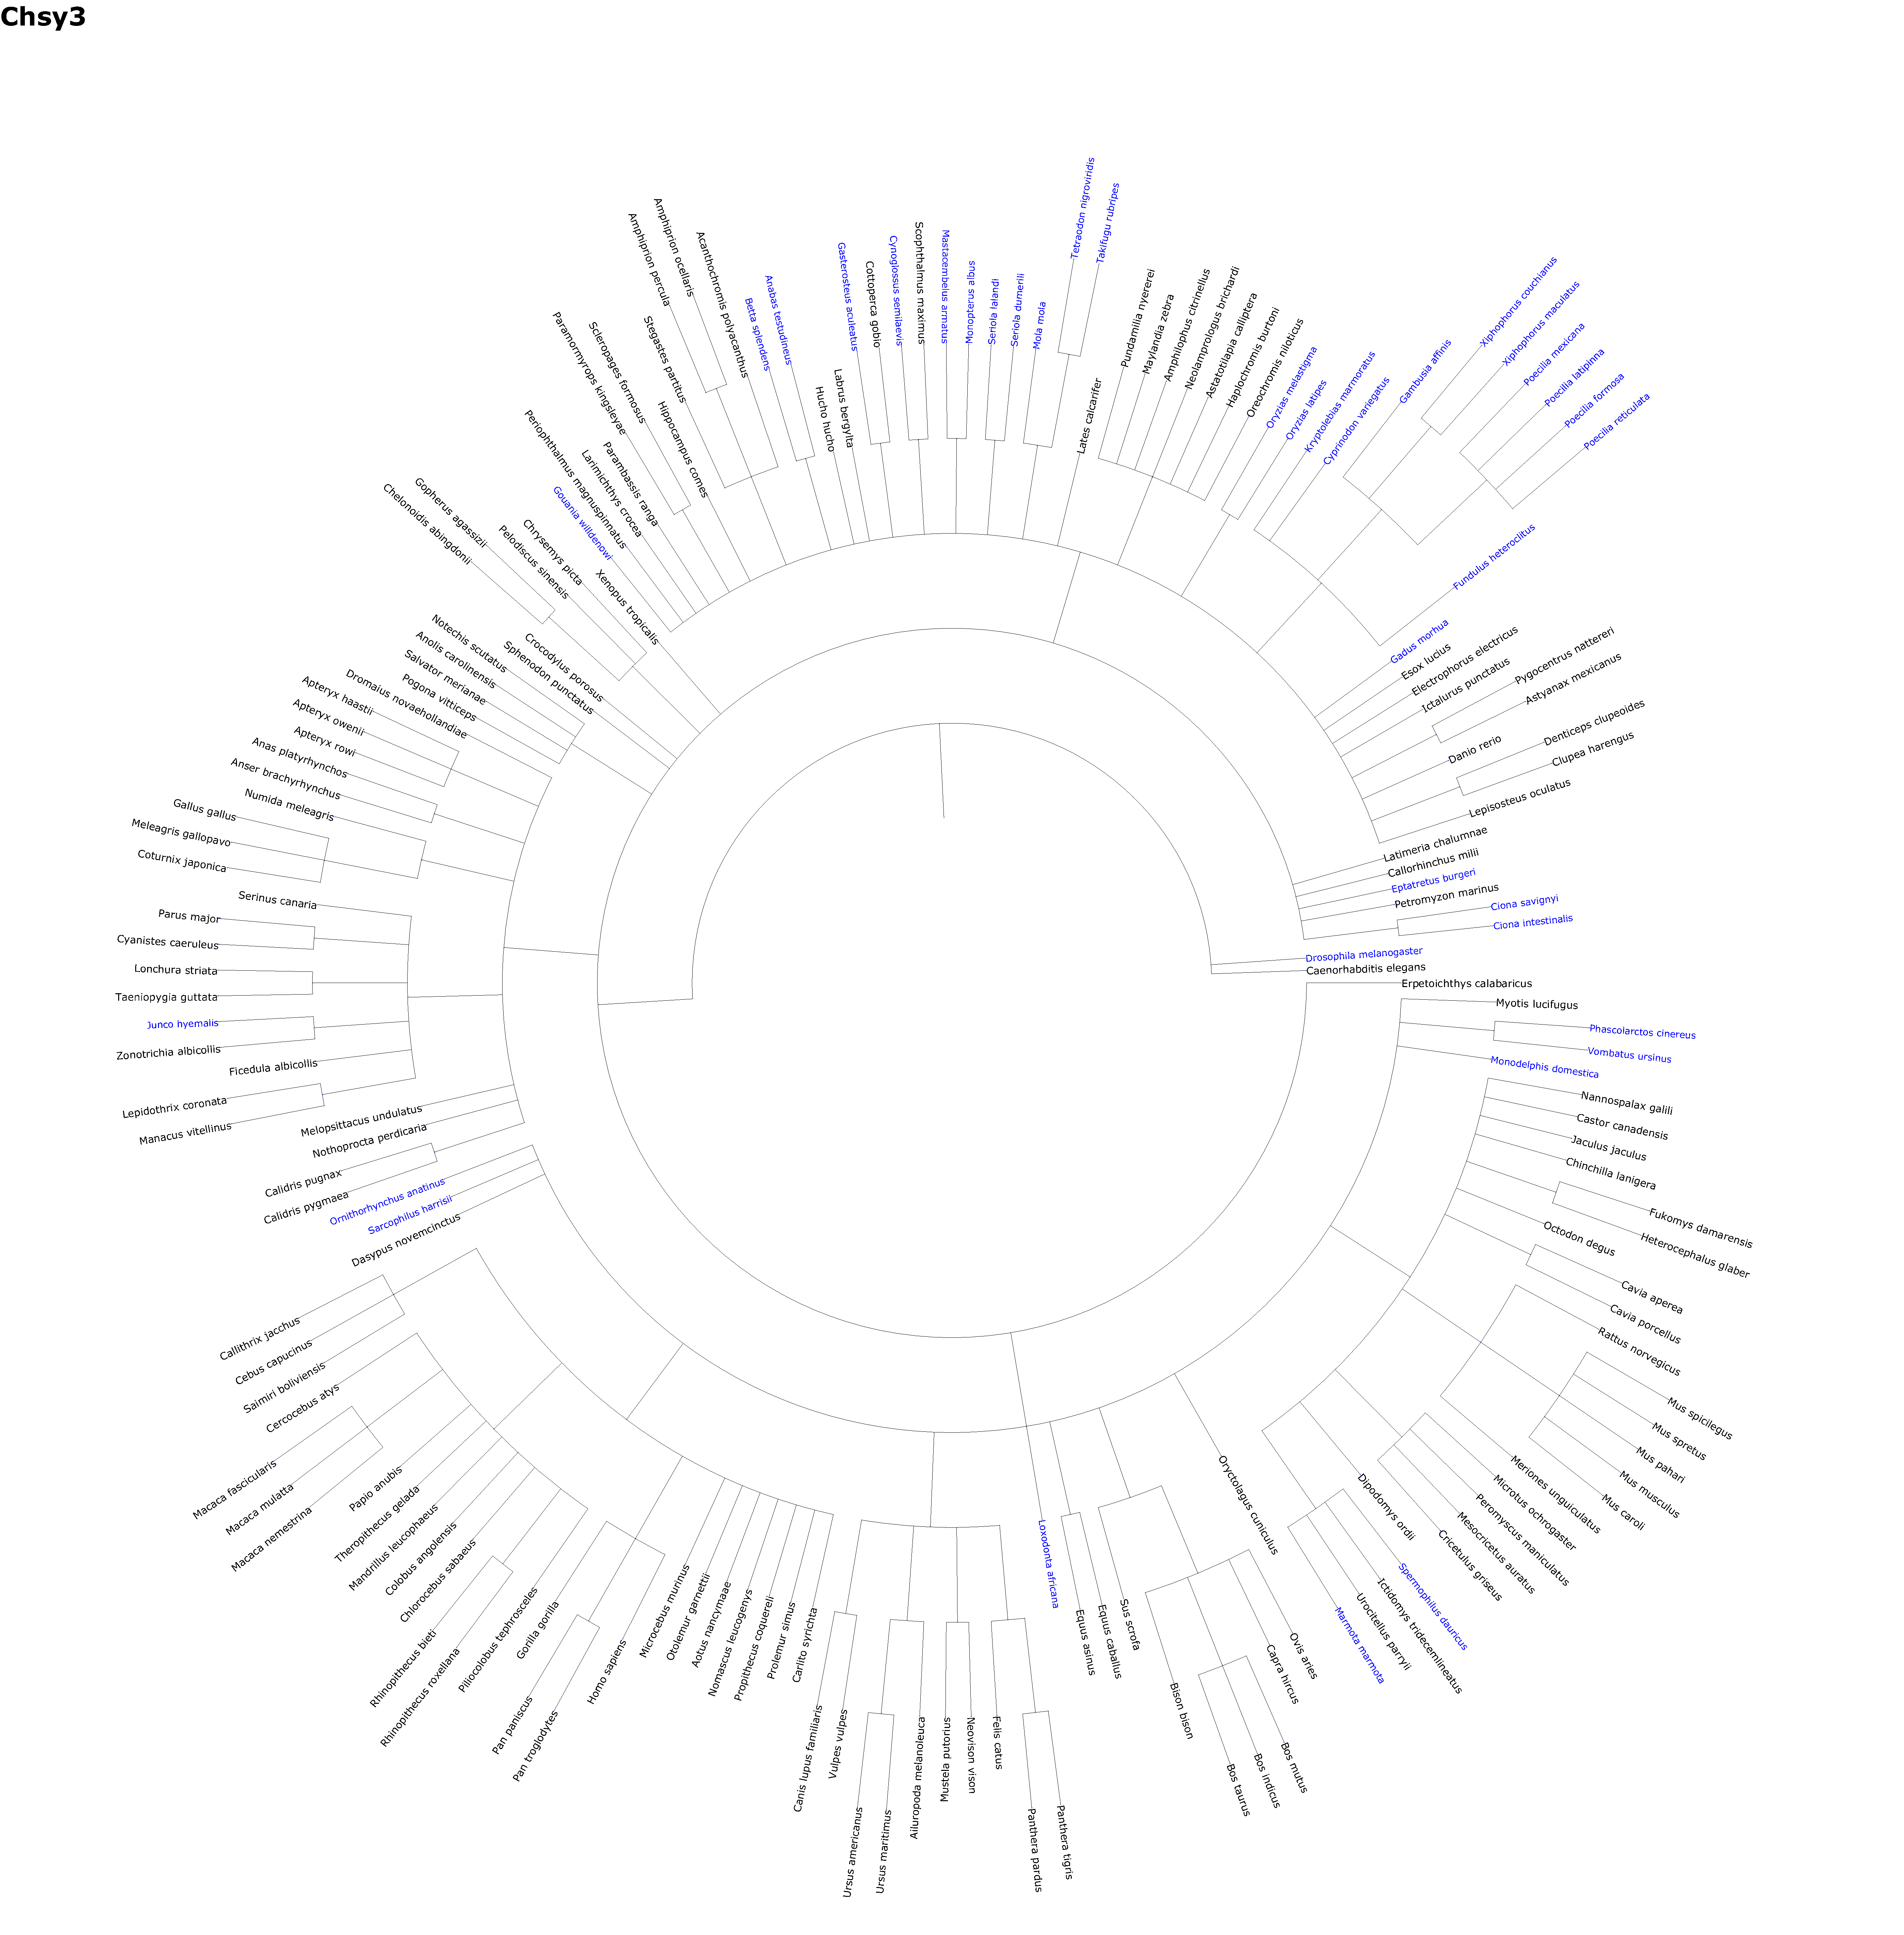
\includegraphics[height=7in,trim={0 0 0 3in},clip]{./appendix_images/trees/Chsy3.pdf}}
\caption{\textbf{The gene tree for \textit{Sumf2}.}}
\label{sup_fig_17}
\end{figure}

\begin{figure}[H]
\centering
\makebox[\textwidth][c]{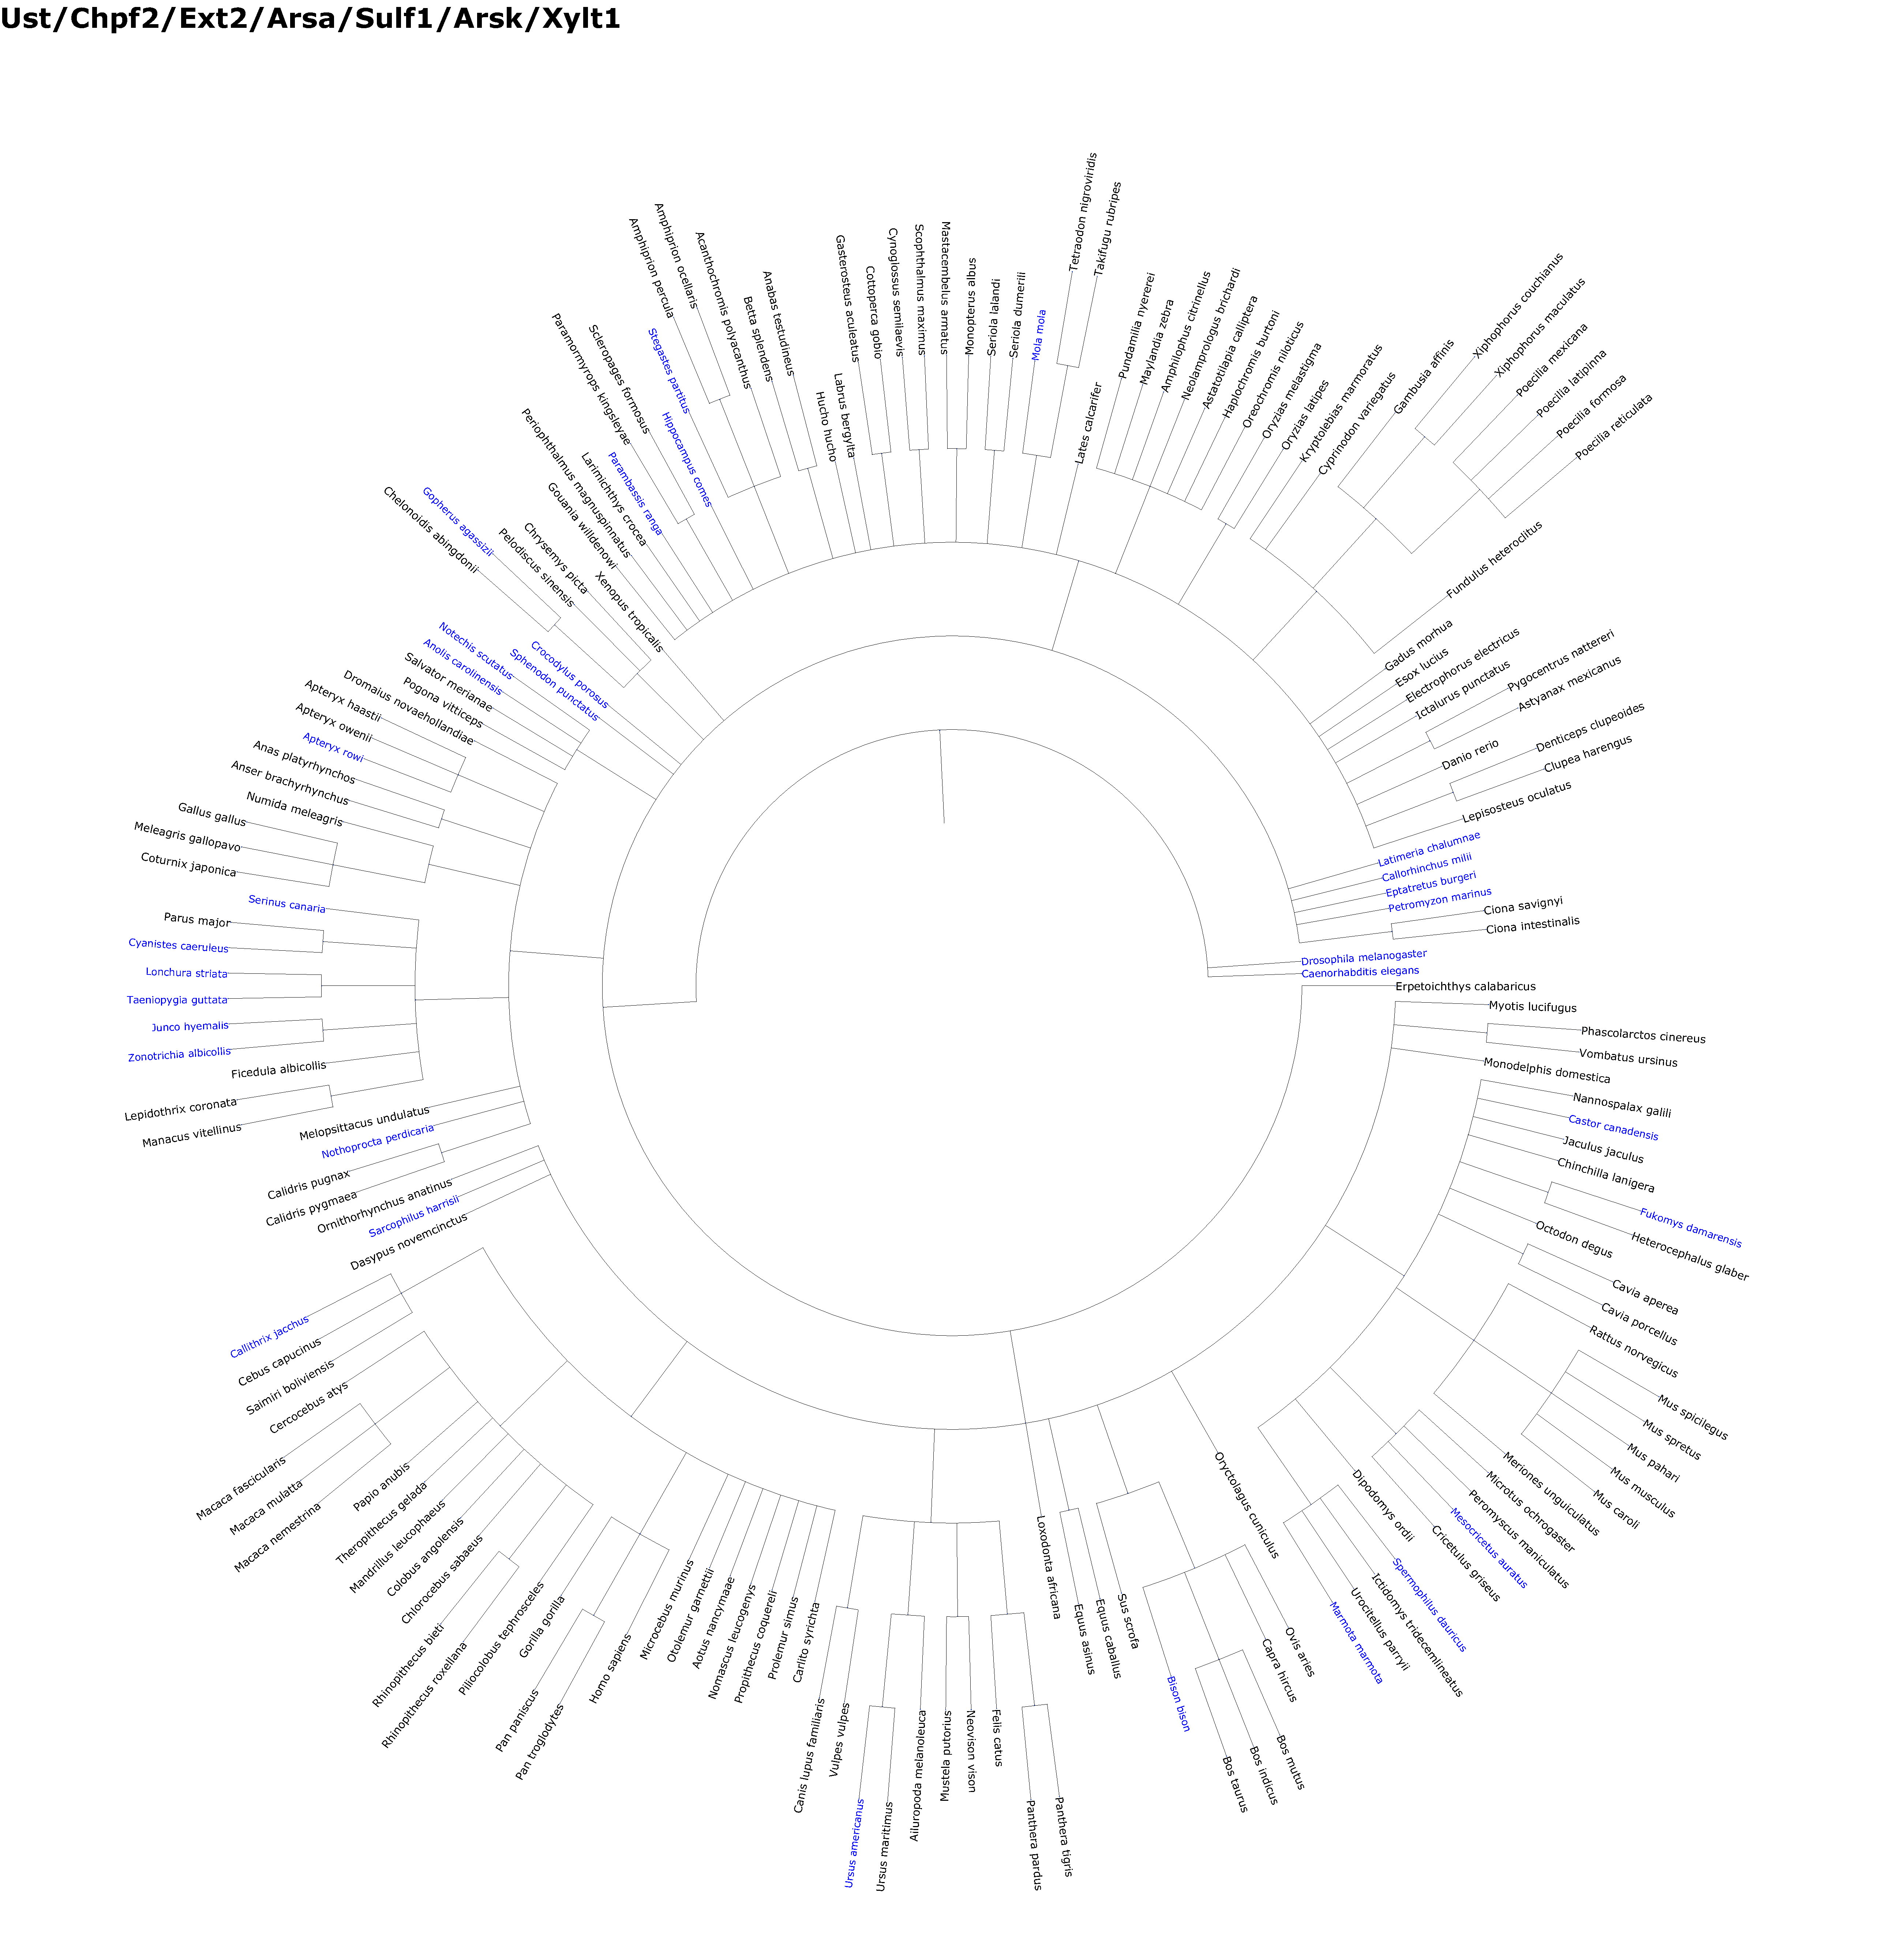
\includegraphics[height=7in,trim={0 0 0 3in},clip]{./appendix_images/trees/Ust_Chpf2_Ext2_Arsa_Sulf1_Arsk_Xylt1.pdf}}
\caption{\textbf{The gene tree for \textit{Ust, Chpf2, Ext2, Arsa, Sulf1, Arsk} and \textit{Xylt1}.}}
\label{sup_fig_18}
\end{figure}

\section{dN/dS}
This section includes supplementary material generated for visualizing the dN/dS ratios for all the significant organisms chosen to analyze in this study.

\begin{figure}[H]
\centering
\makebox[\textwidth][c]{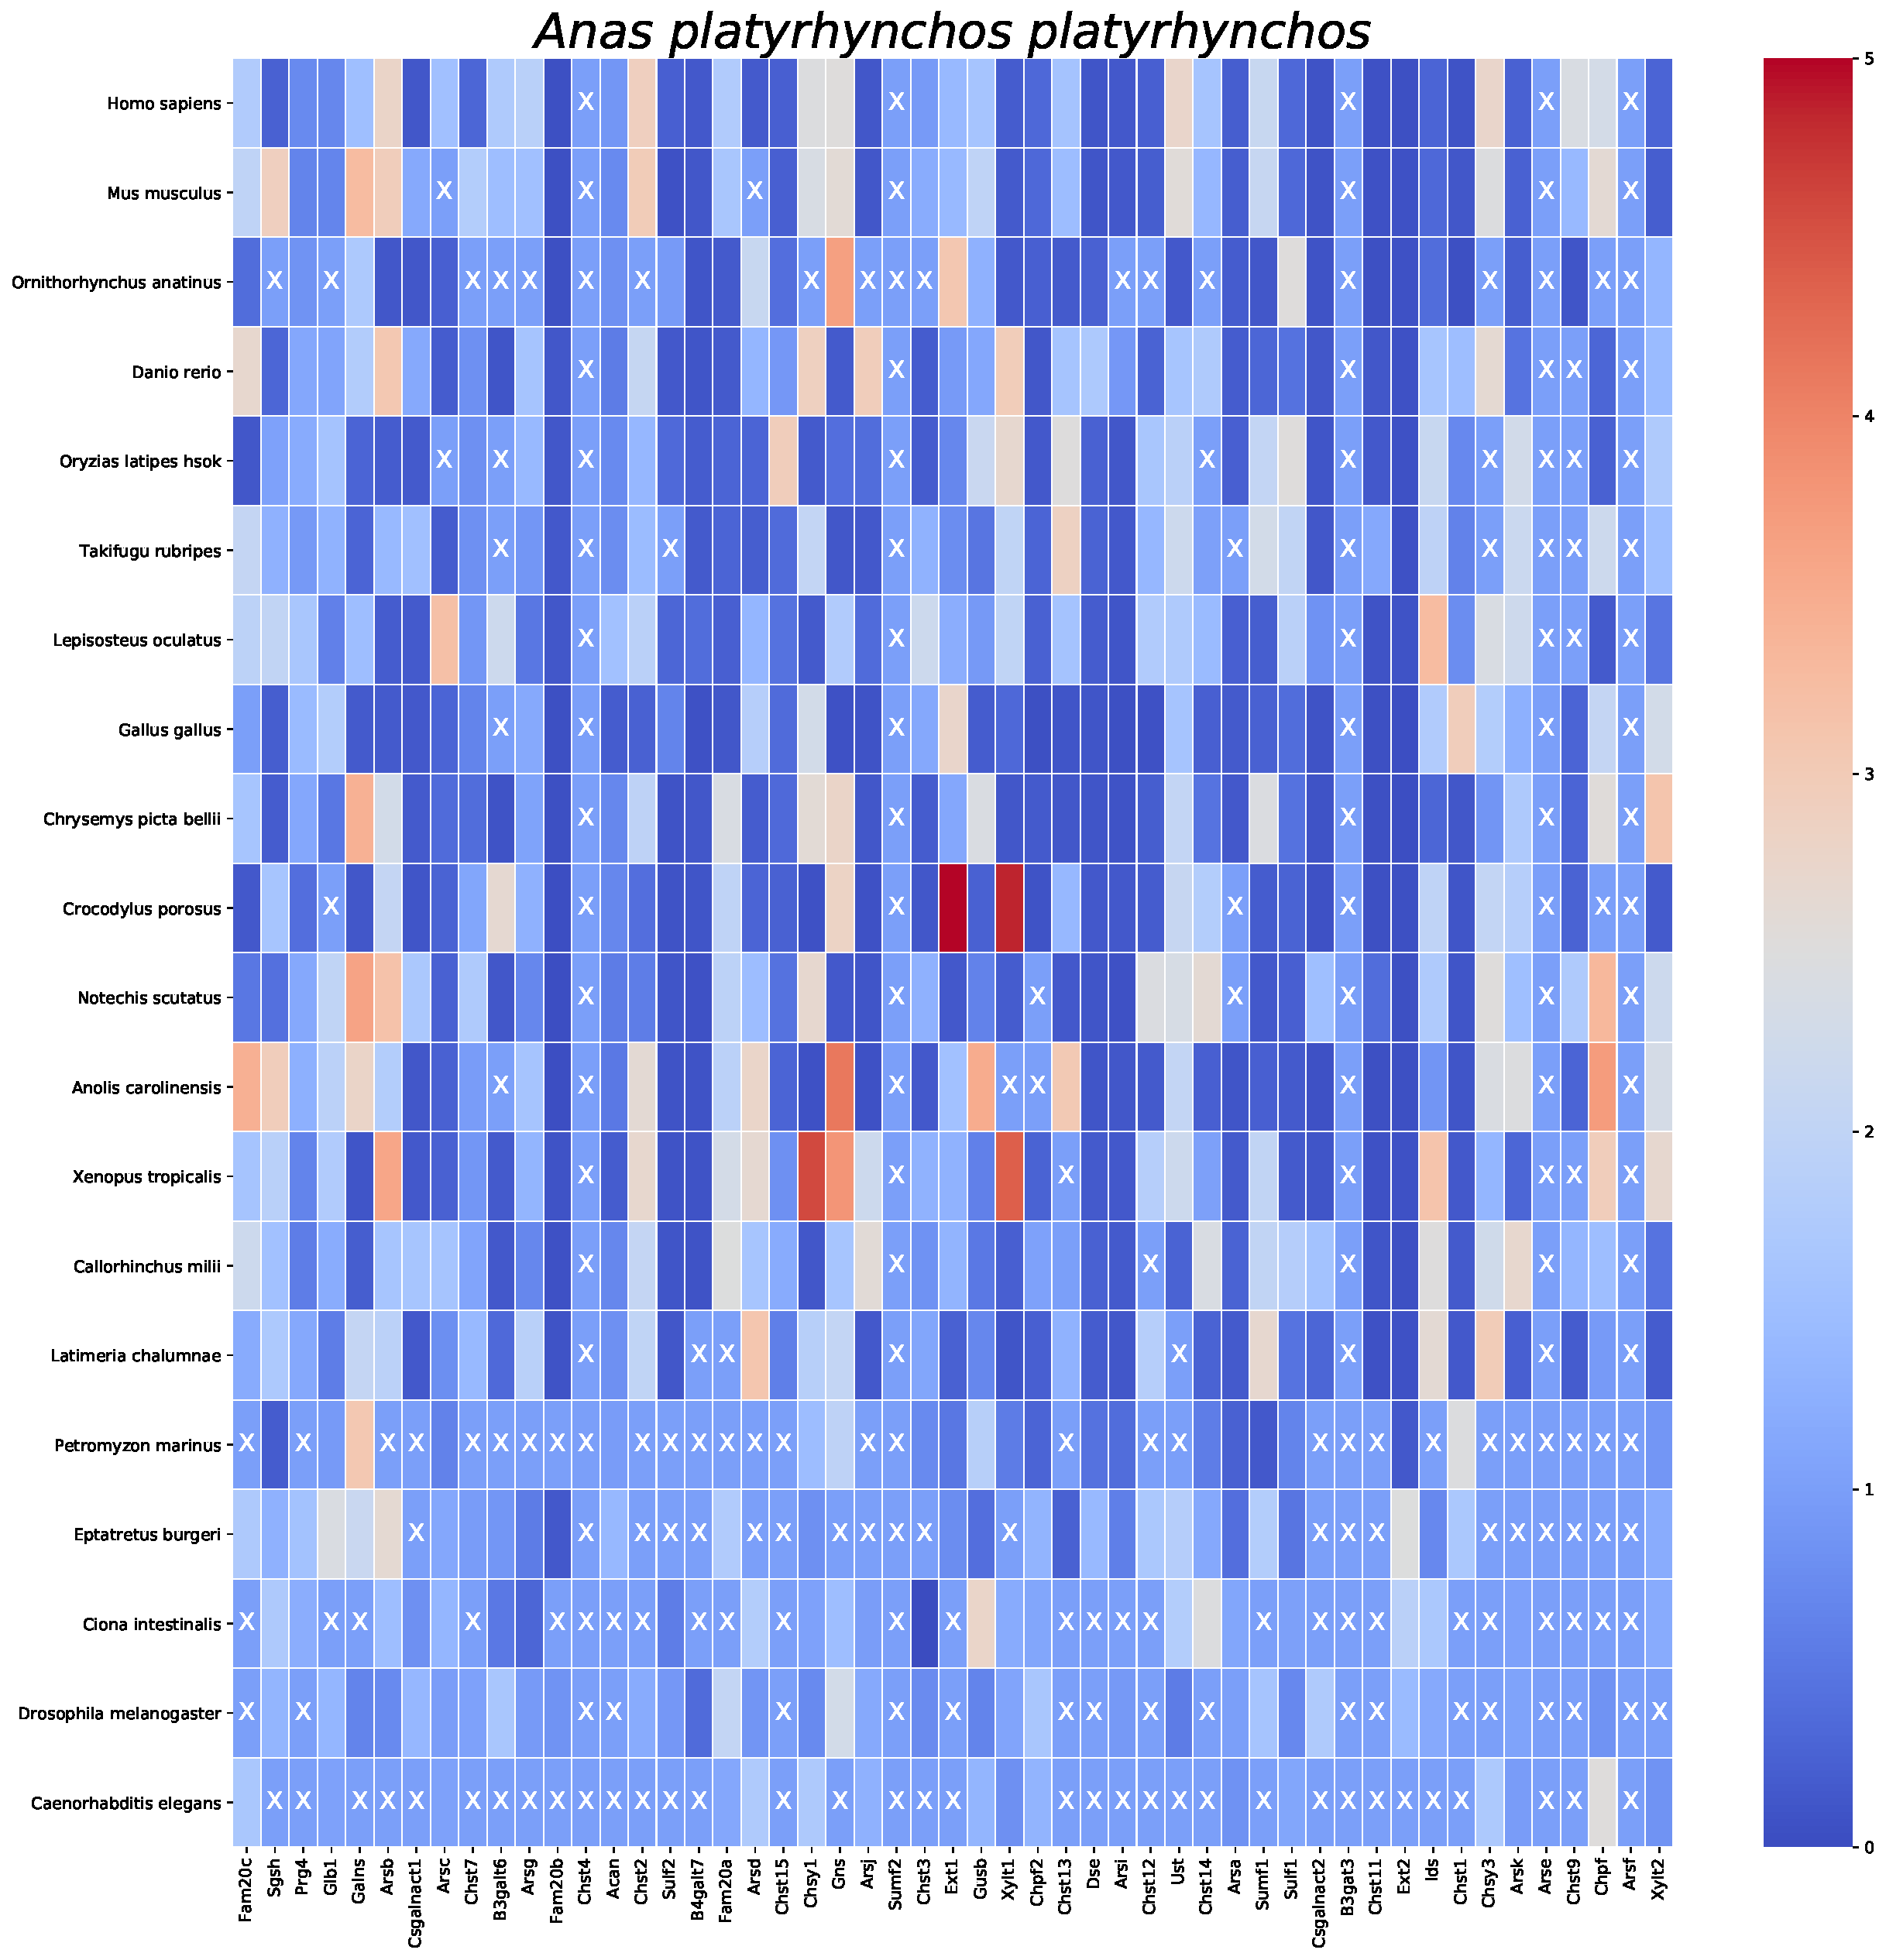
\includegraphics[height=7in,trim={0 0 0 0in},clip]{./appendix_images/dnds/anas_platyrhynchos_platyrhynchos.pdf}}
\caption{\textbf{dN/dS 2D grid for \textit{Anas platyrhynchos} computed against the other significant organisms.} The intensity values represent the dN/dS ratio - values lighter in colour are less than 1 and purifying selection while values darker in colour are greater than 1 and represent positive selection.}
\label{sup_fig_19}
\end{figure}

\begin{figure}[H]
\centering
\makebox[\textwidth][c]{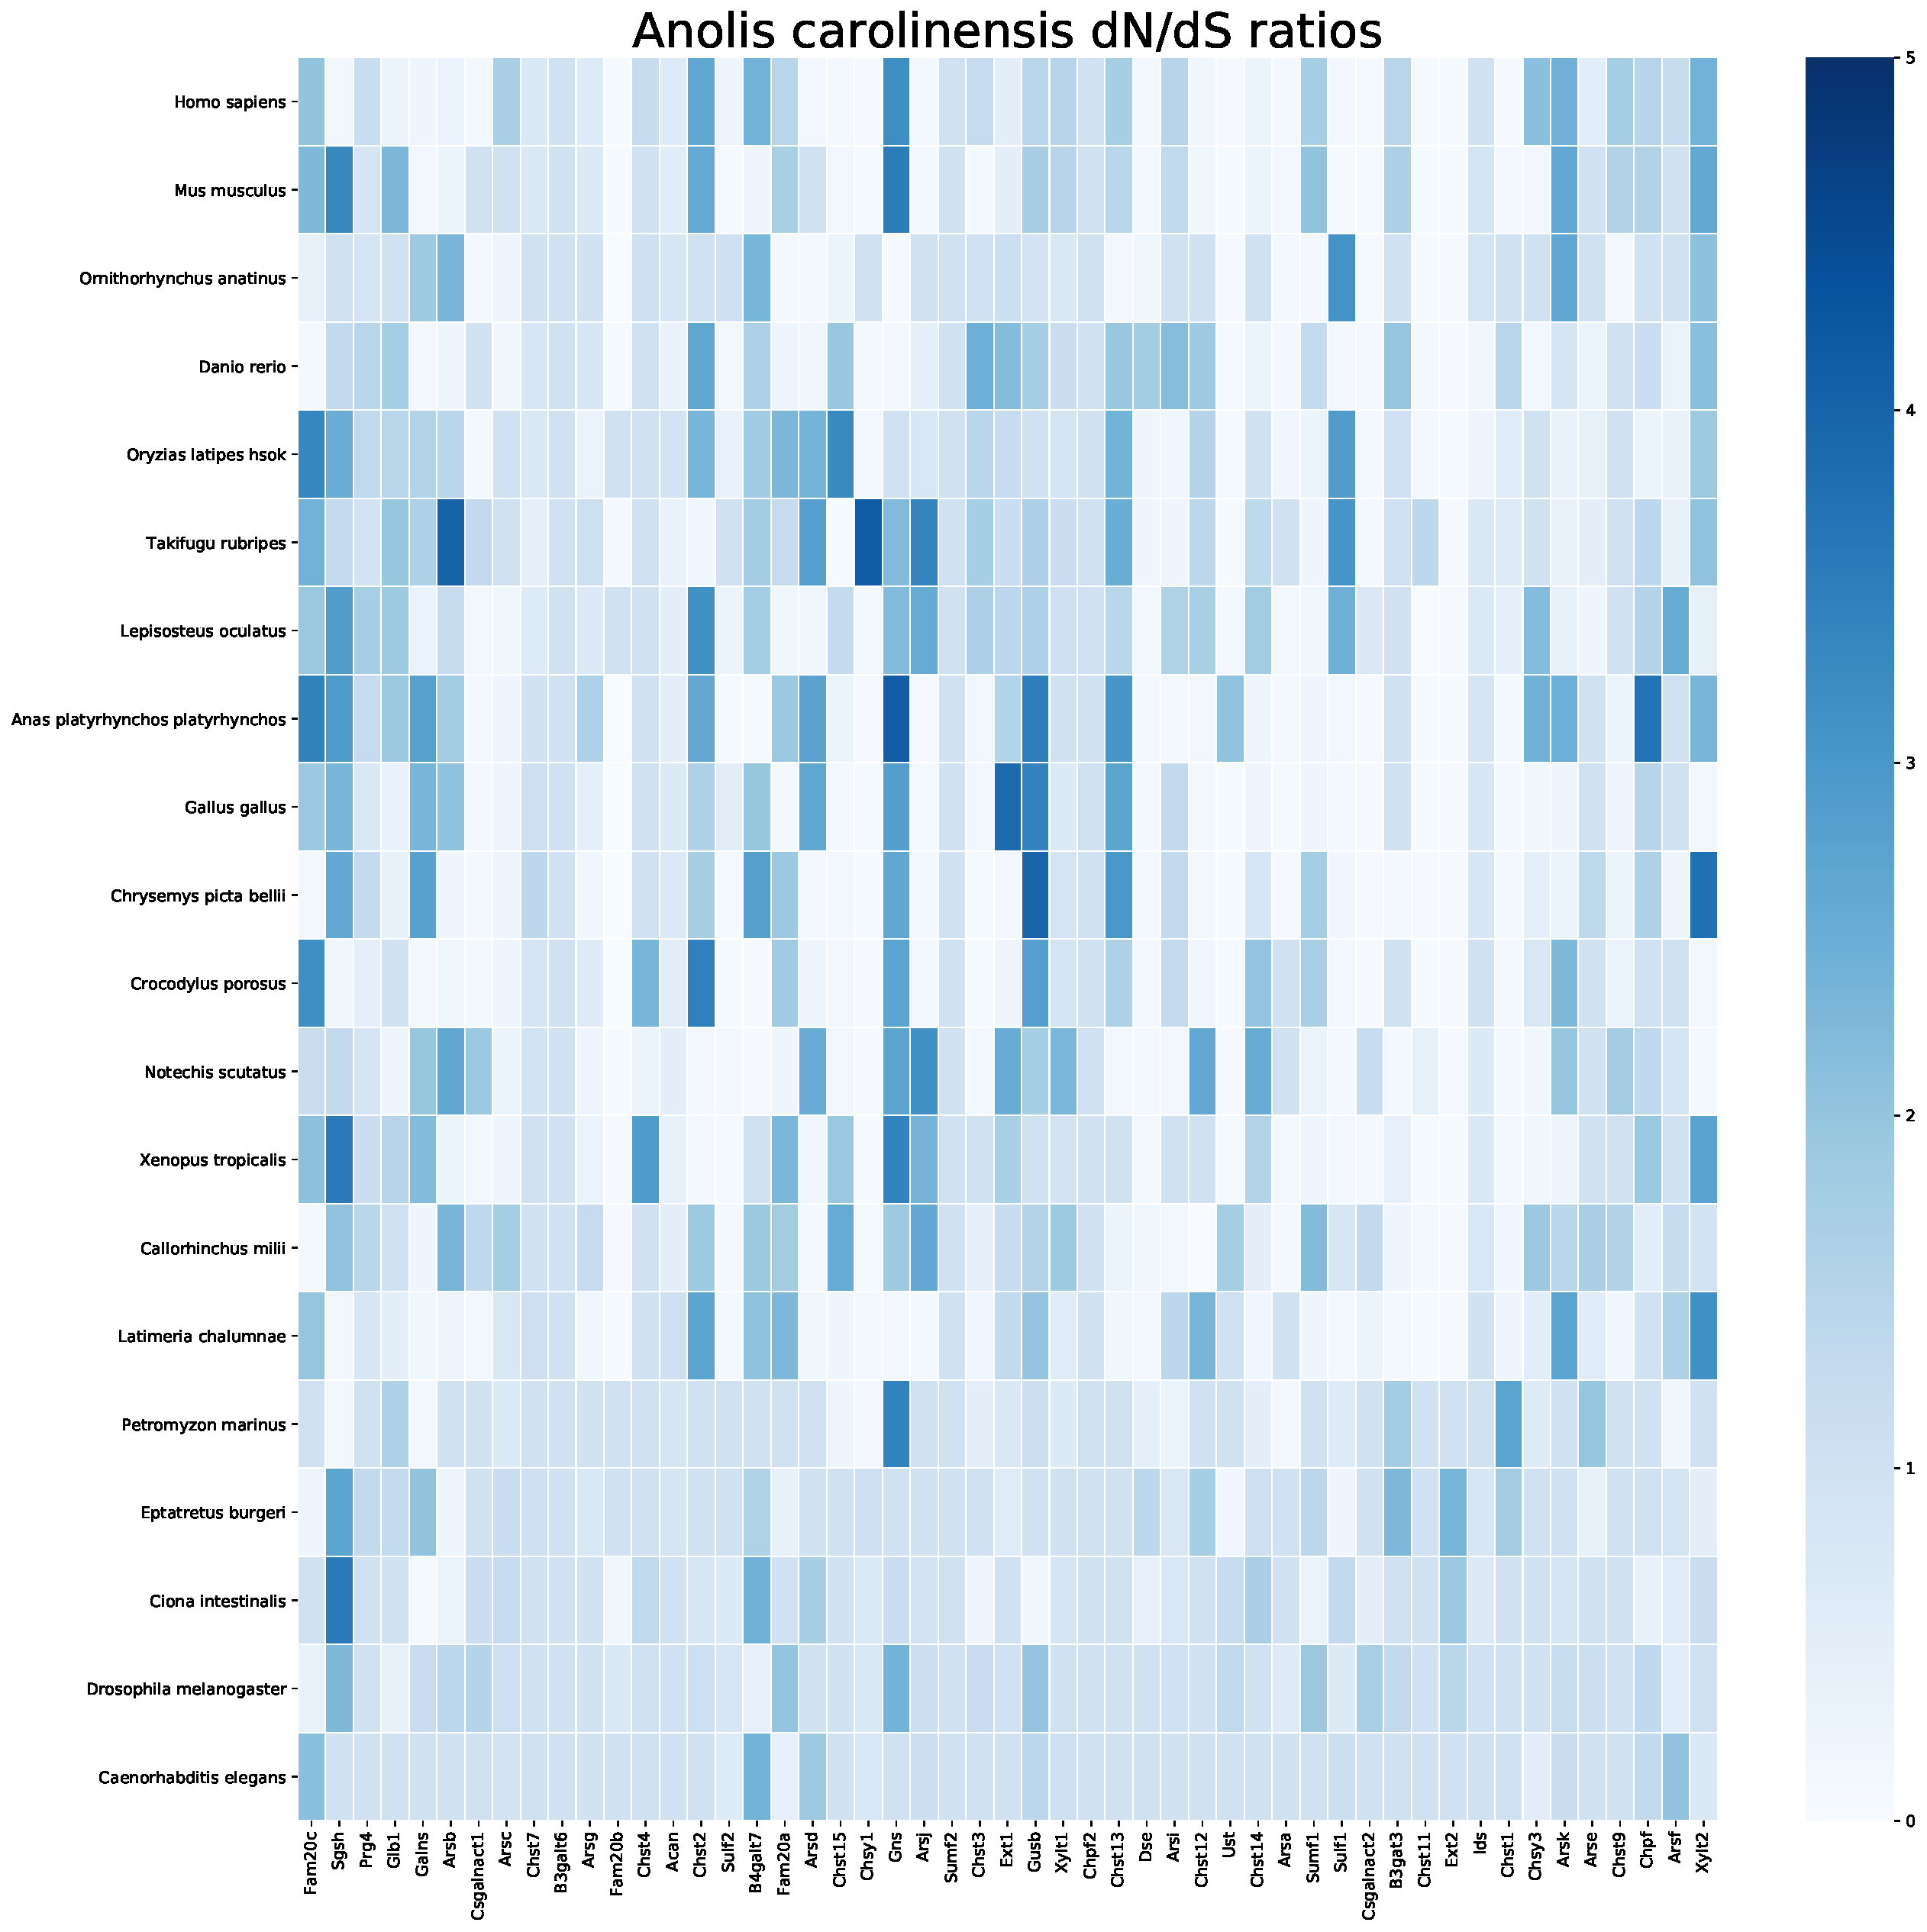
\includegraphics[height=7in,trim={0 0 0 0in},clip]{./appendix_images/dnds/anolis_carolinensis.pdf}}
\caption{\textbf{dN/dS 2D grid for \textit{Anolis Carolinensis} computed against the other significant organisms.} The intensity values represent the dN/dS ratio - values lighter in colour are less than 1 and purifying selection while values darker in colour are greater than 1 and represent positive selection.}
\label{sup_fig_20}
\end{figure}

\begin{figure}[H]
\centering
\makebox[\textwidth][c]{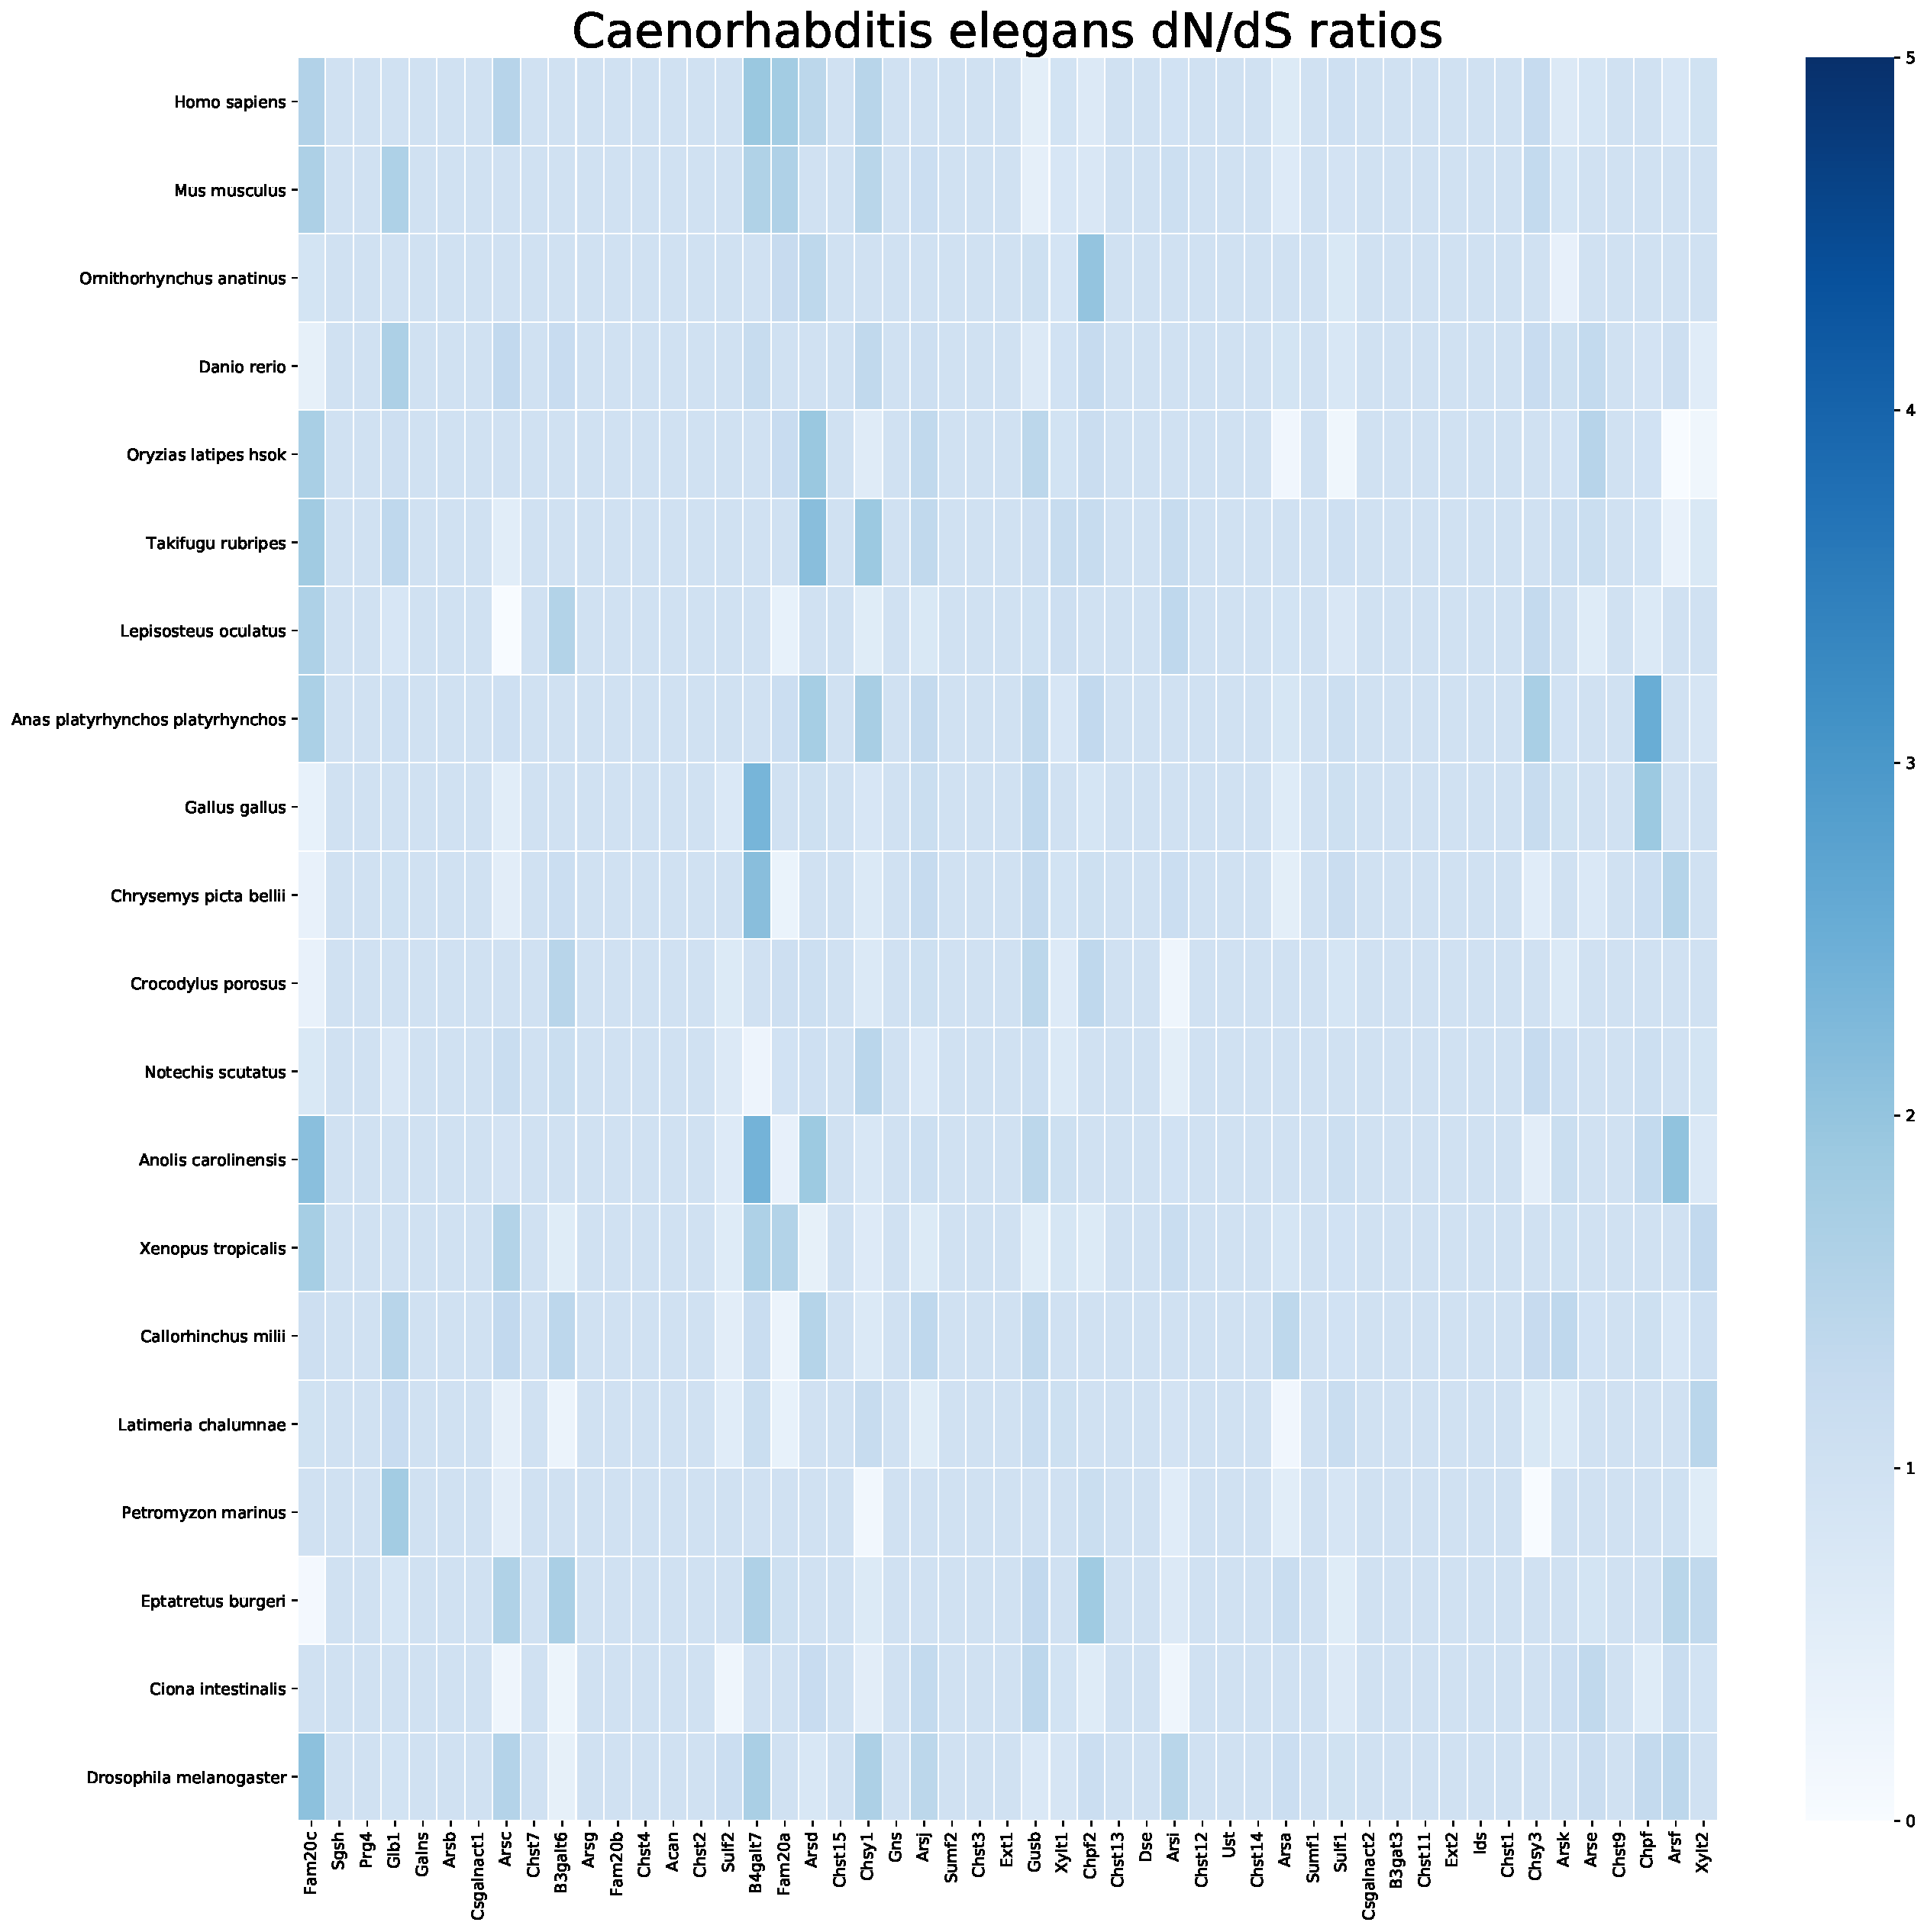
\includegraphics[height=7in,trim={0 0 0 0in},clip]{./appendix_images/dnds/caenorhabditis_elegans.pdf}}
\caption{\textbf{dN/dS 2D grid for \textit{Caenorhabditis elegans} computed against the other significant organisms.} The intensity values represent the dN/dS ratio - values lighter in colour are less than 1 and purifying selection while values darker in colour are greater than 1 and represent positive selection.}
\label{sup_fig_21}
\end{figure}

\begin{figure}[H]
\centering
\makebox[\textwidth][c]{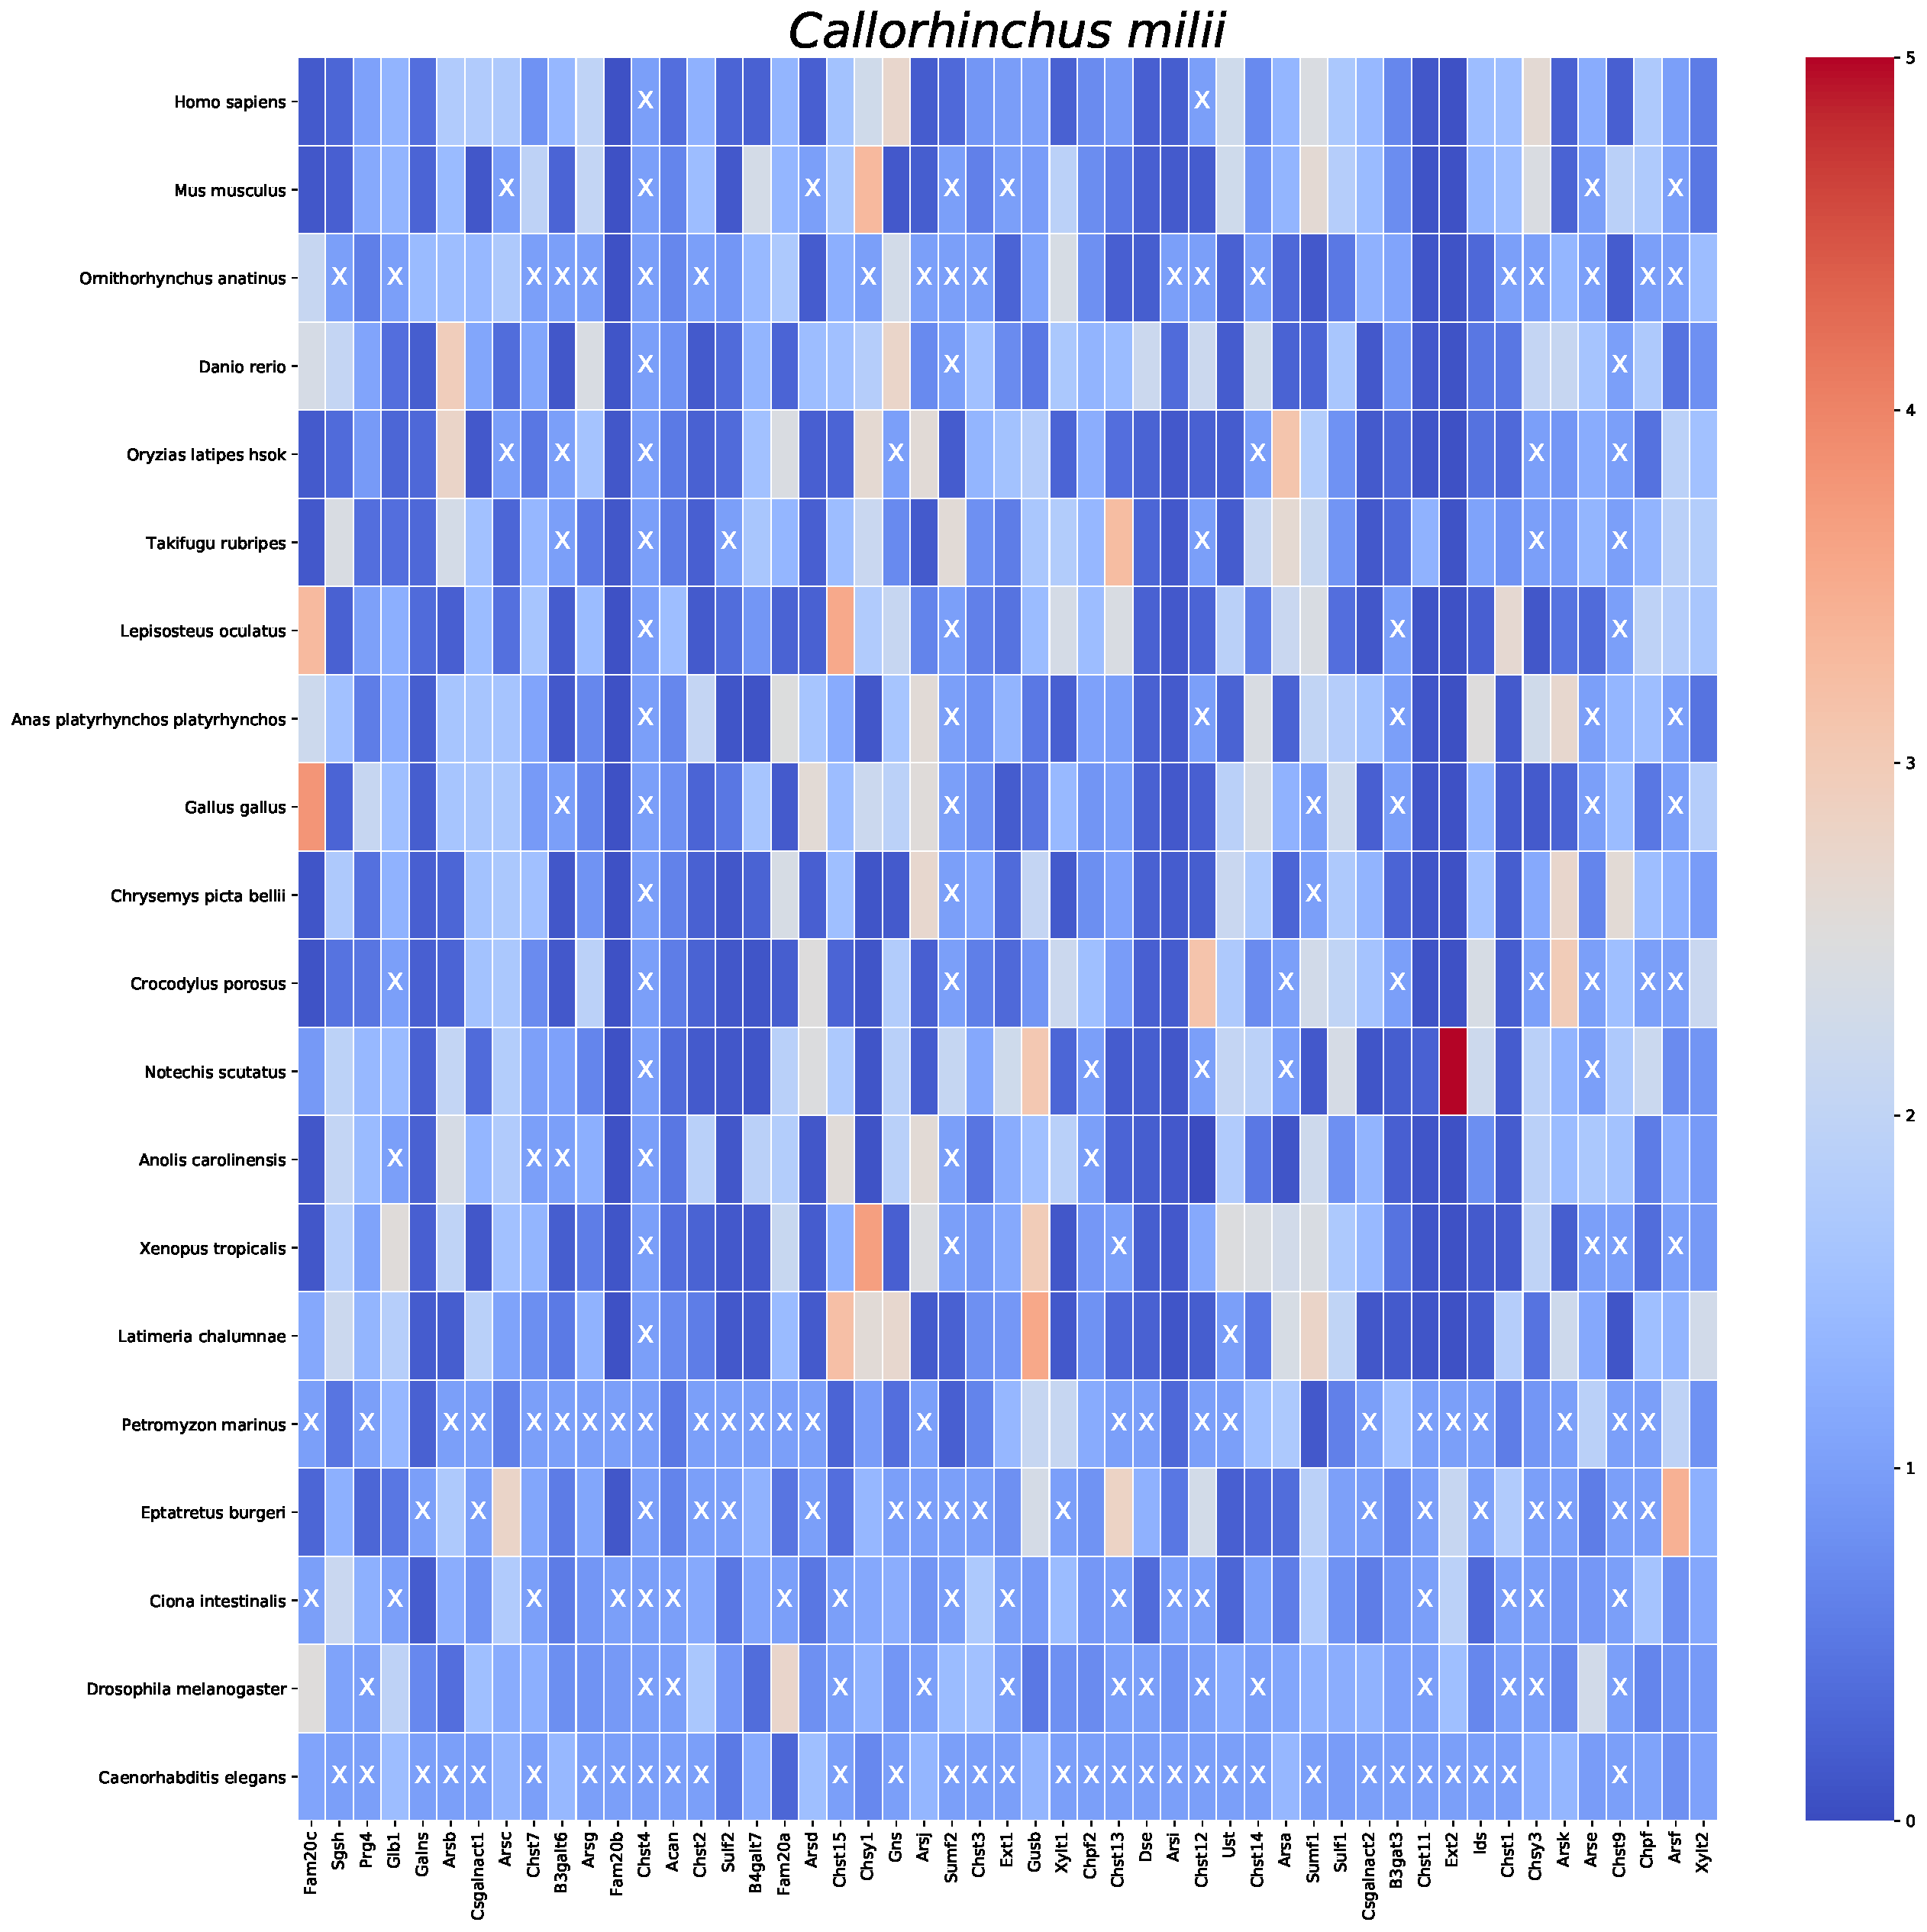
\includegraphics[height=7in,trim={0 0 0 0in},clip]{./appendix_images/dnds/callorhinchus_milii.pdf}}
\caption{\textbf{dN/dS 2D grid for \textit{Callorhinchus millii} computed against the other significant organisms.} The intensity values represent the dN/dS ratio - values lighter in colour are less than 1 and purifying selection while values darker in colour are greater than 1 and represent positive selection.}
\label{sup_fig_19}
\end{figure}

\begin{figure}[H]
\centering
\makebox[\textwidth][c]{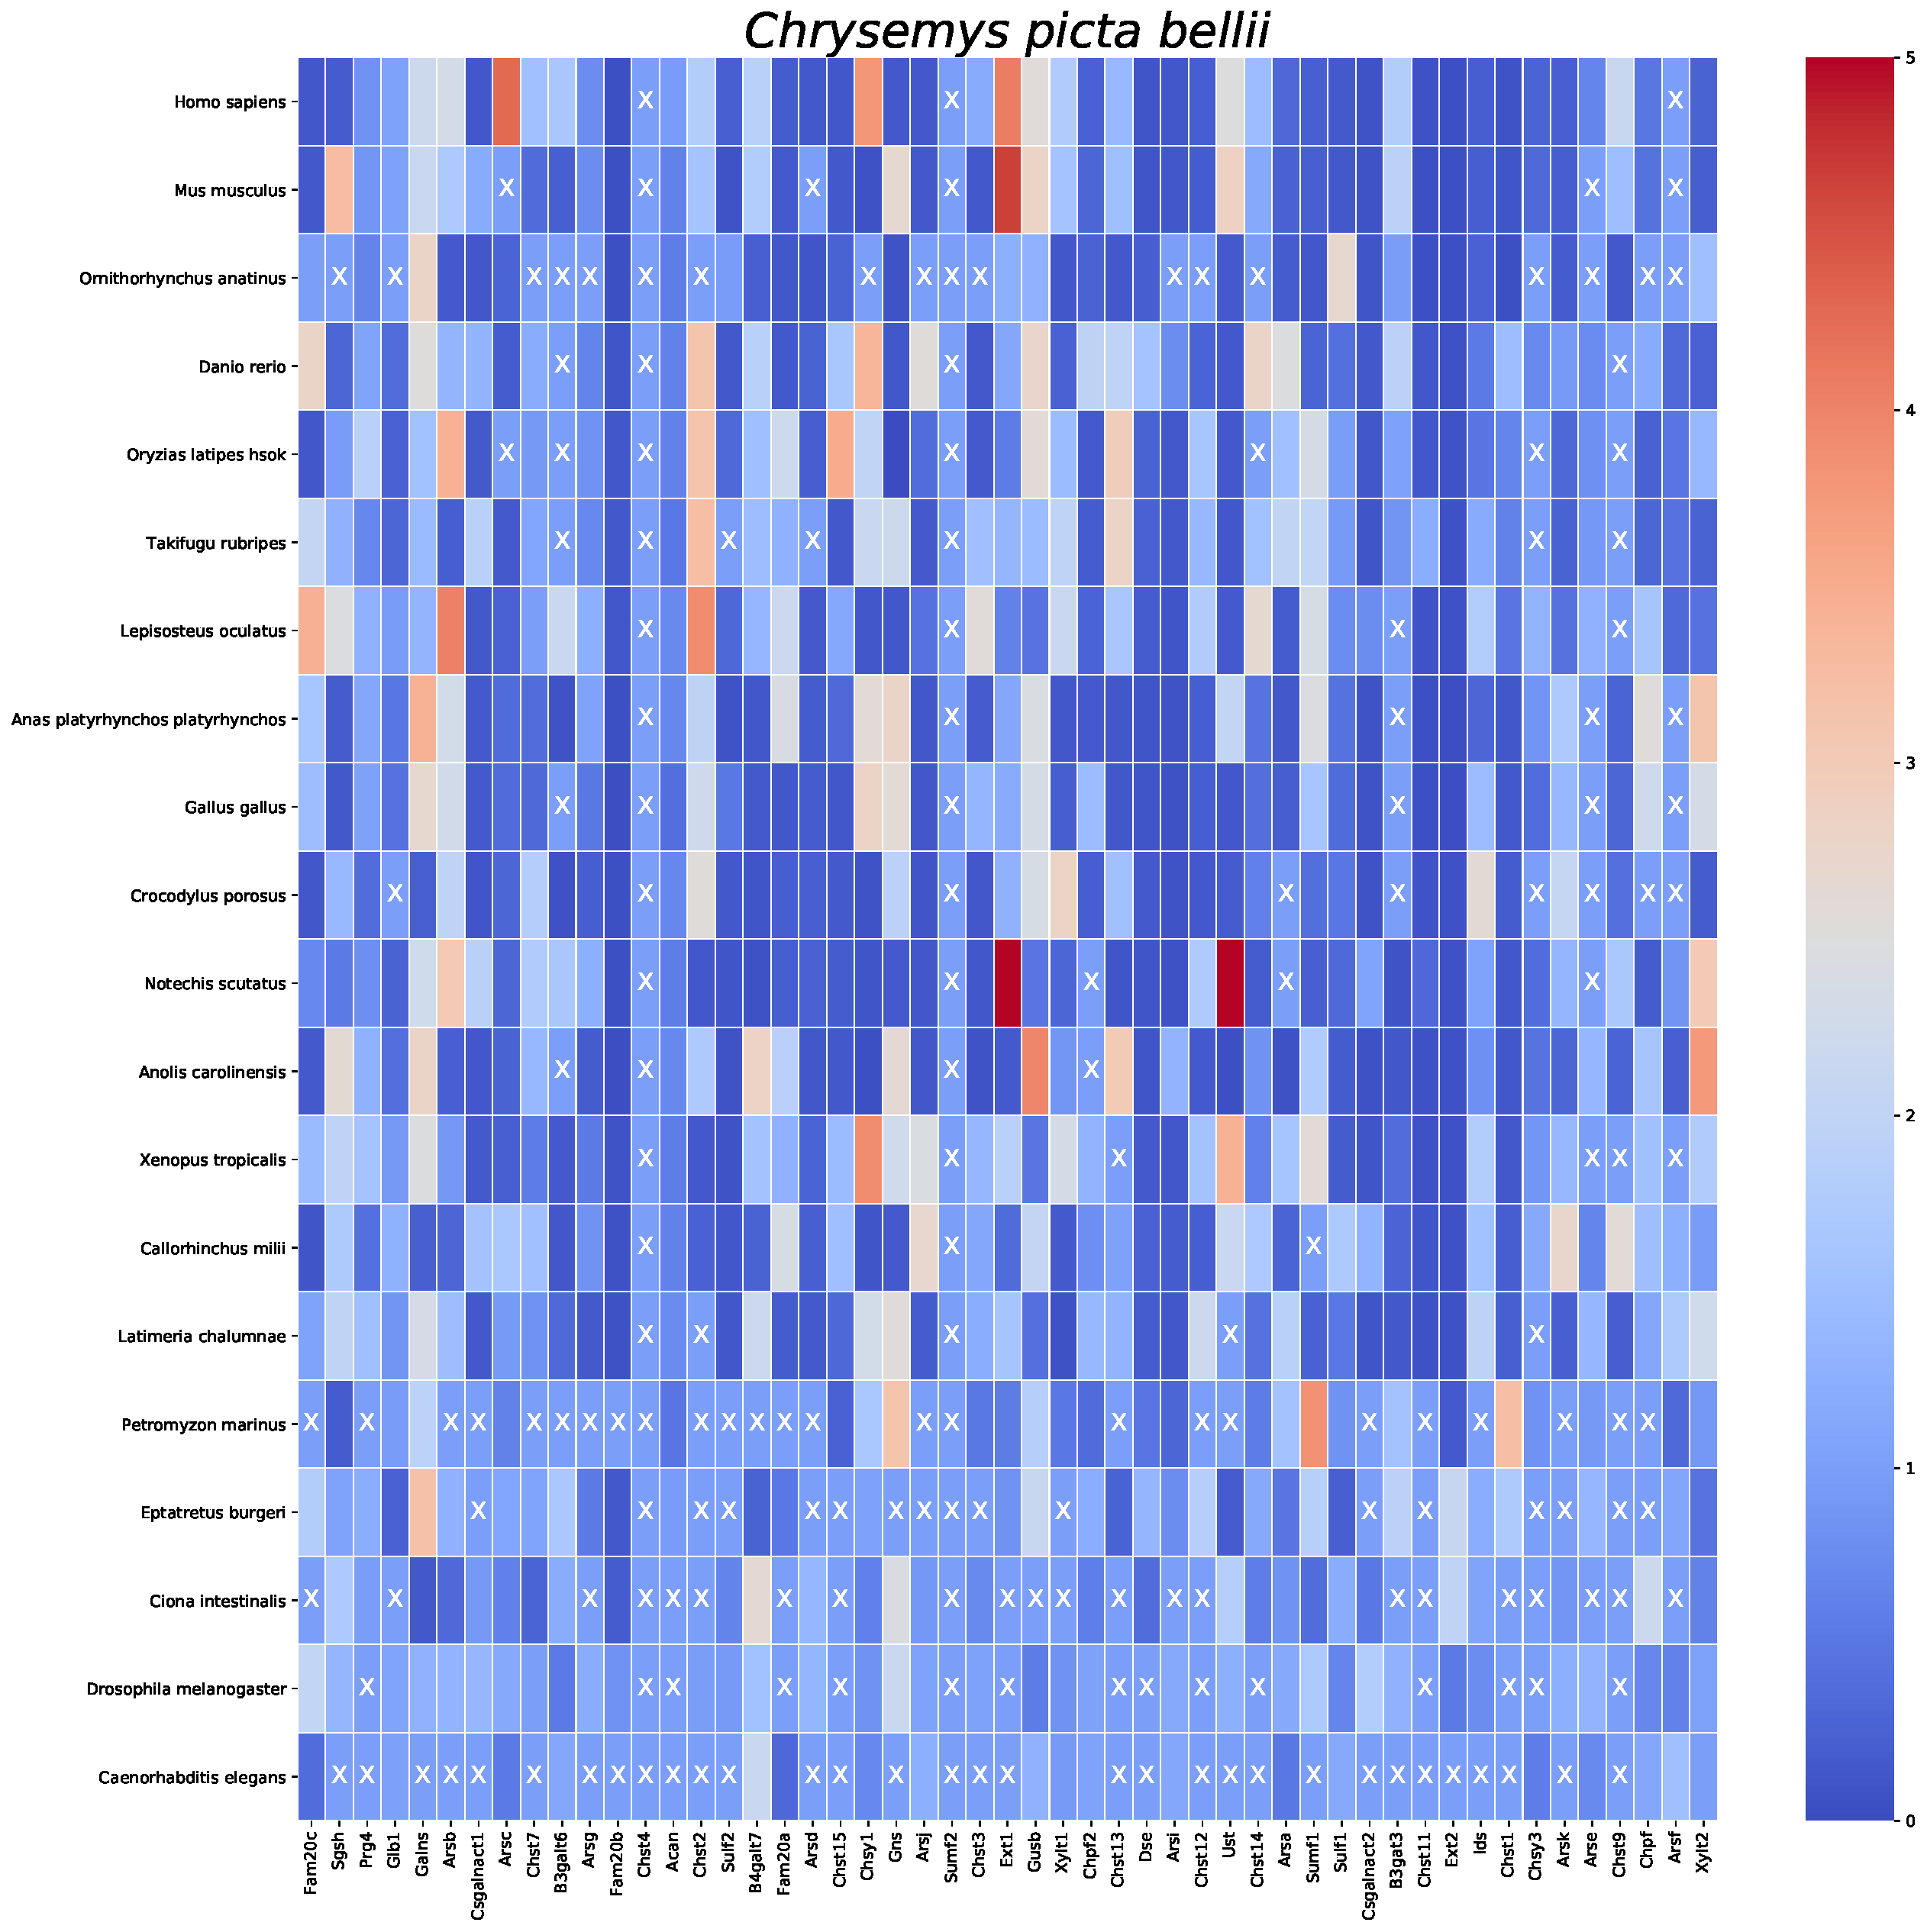
\includegraphics[height=7in,trim={0 0 0 0in},clip]{./appendix_images/dnds/chrysemys_picta_bellii.pdf}}
\caption{\textbf{dN/dS 2D grid for \textit{Chrysemys picta bellii} computed against the other significant organisms.} The intensity values represent the dN/dS ratio - values lighter in colour are less than 1 and purifying selection while values darker in colour are greater than 1 and represent positive selection.}
\label{sup_fig_20}
\end{figure}

\begin{figure}[H]
\centering
\makebox[\textwidth][c]{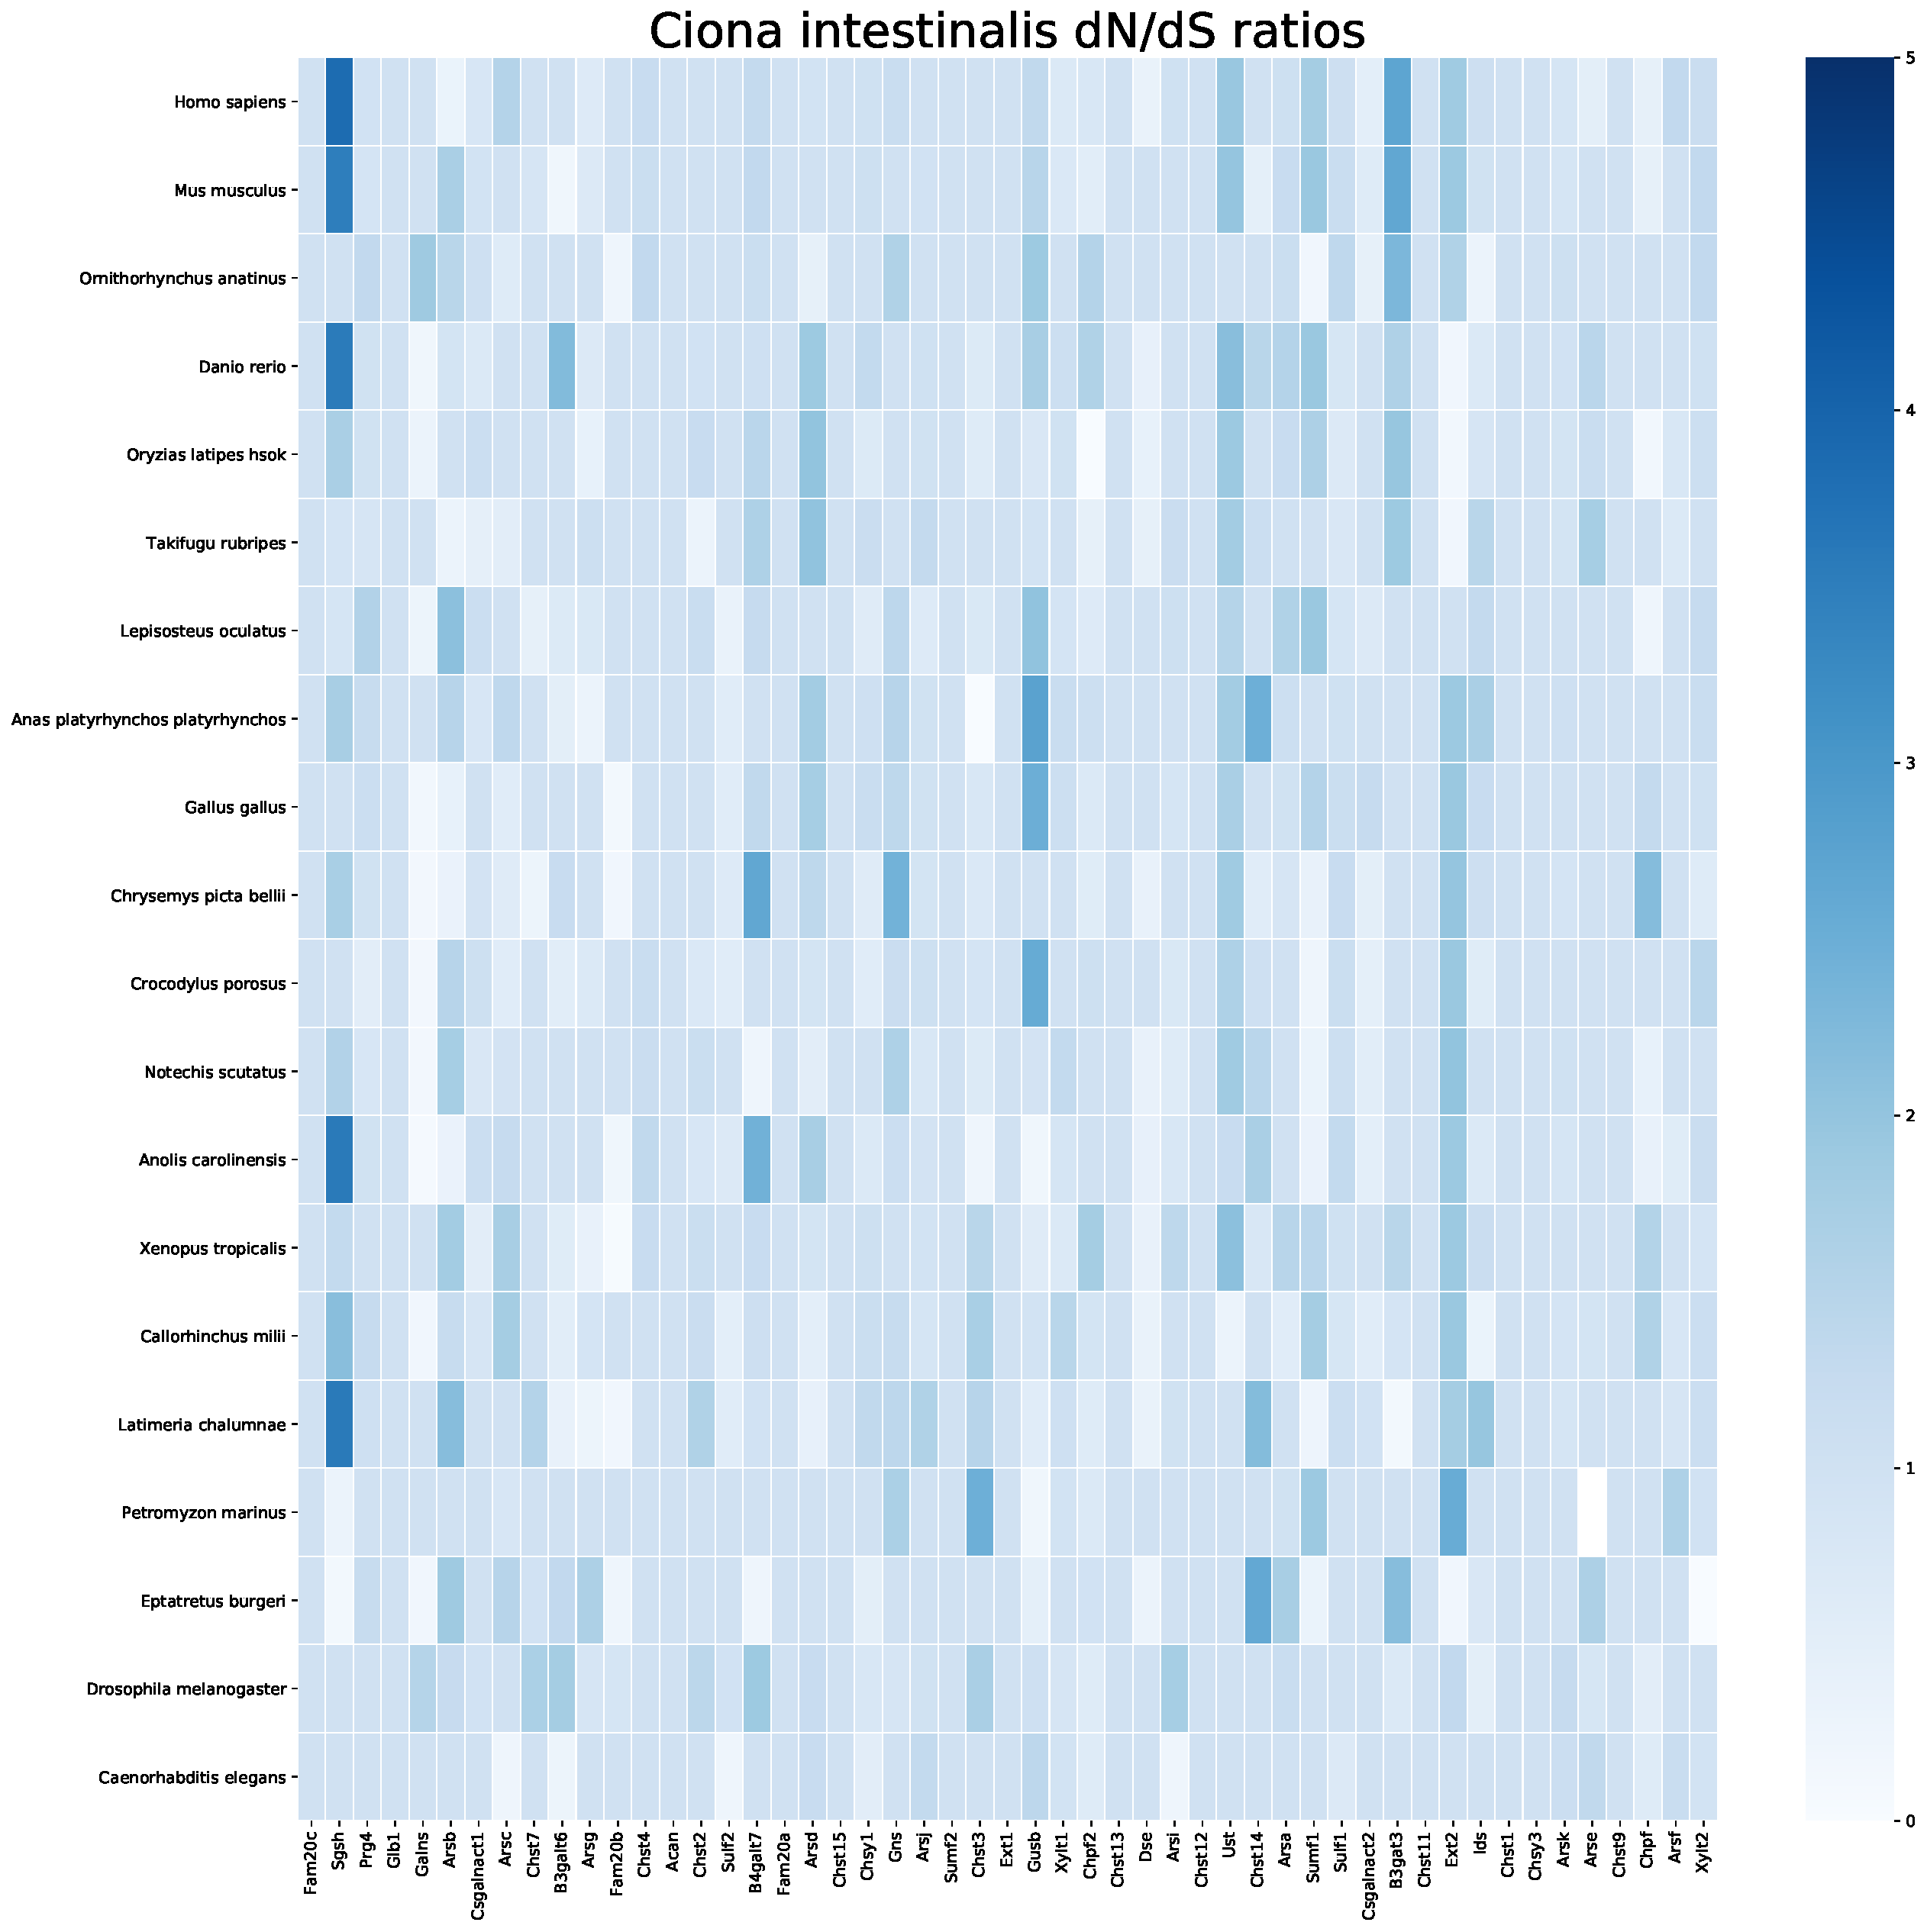
\includegraphics[height=7in,trim={0 0 0 0in},clip]{./appendix_images/dnds/ciona_intestinalis.pdf}}
\caption{\textbf{dN/dS 2D grid for \textit{Ciona intestinalis} computed against the other significant organisms.} The intensity values represent the dN/dS ratio - values lighter in colour are less than 1 and purifying selection while values darker in colour are greater than 1 and represent positive selection.}
\label{sup_fig_21}
\end{figure}

\begin{figure}[H]
\centering
\makebox[\textwidth][c]{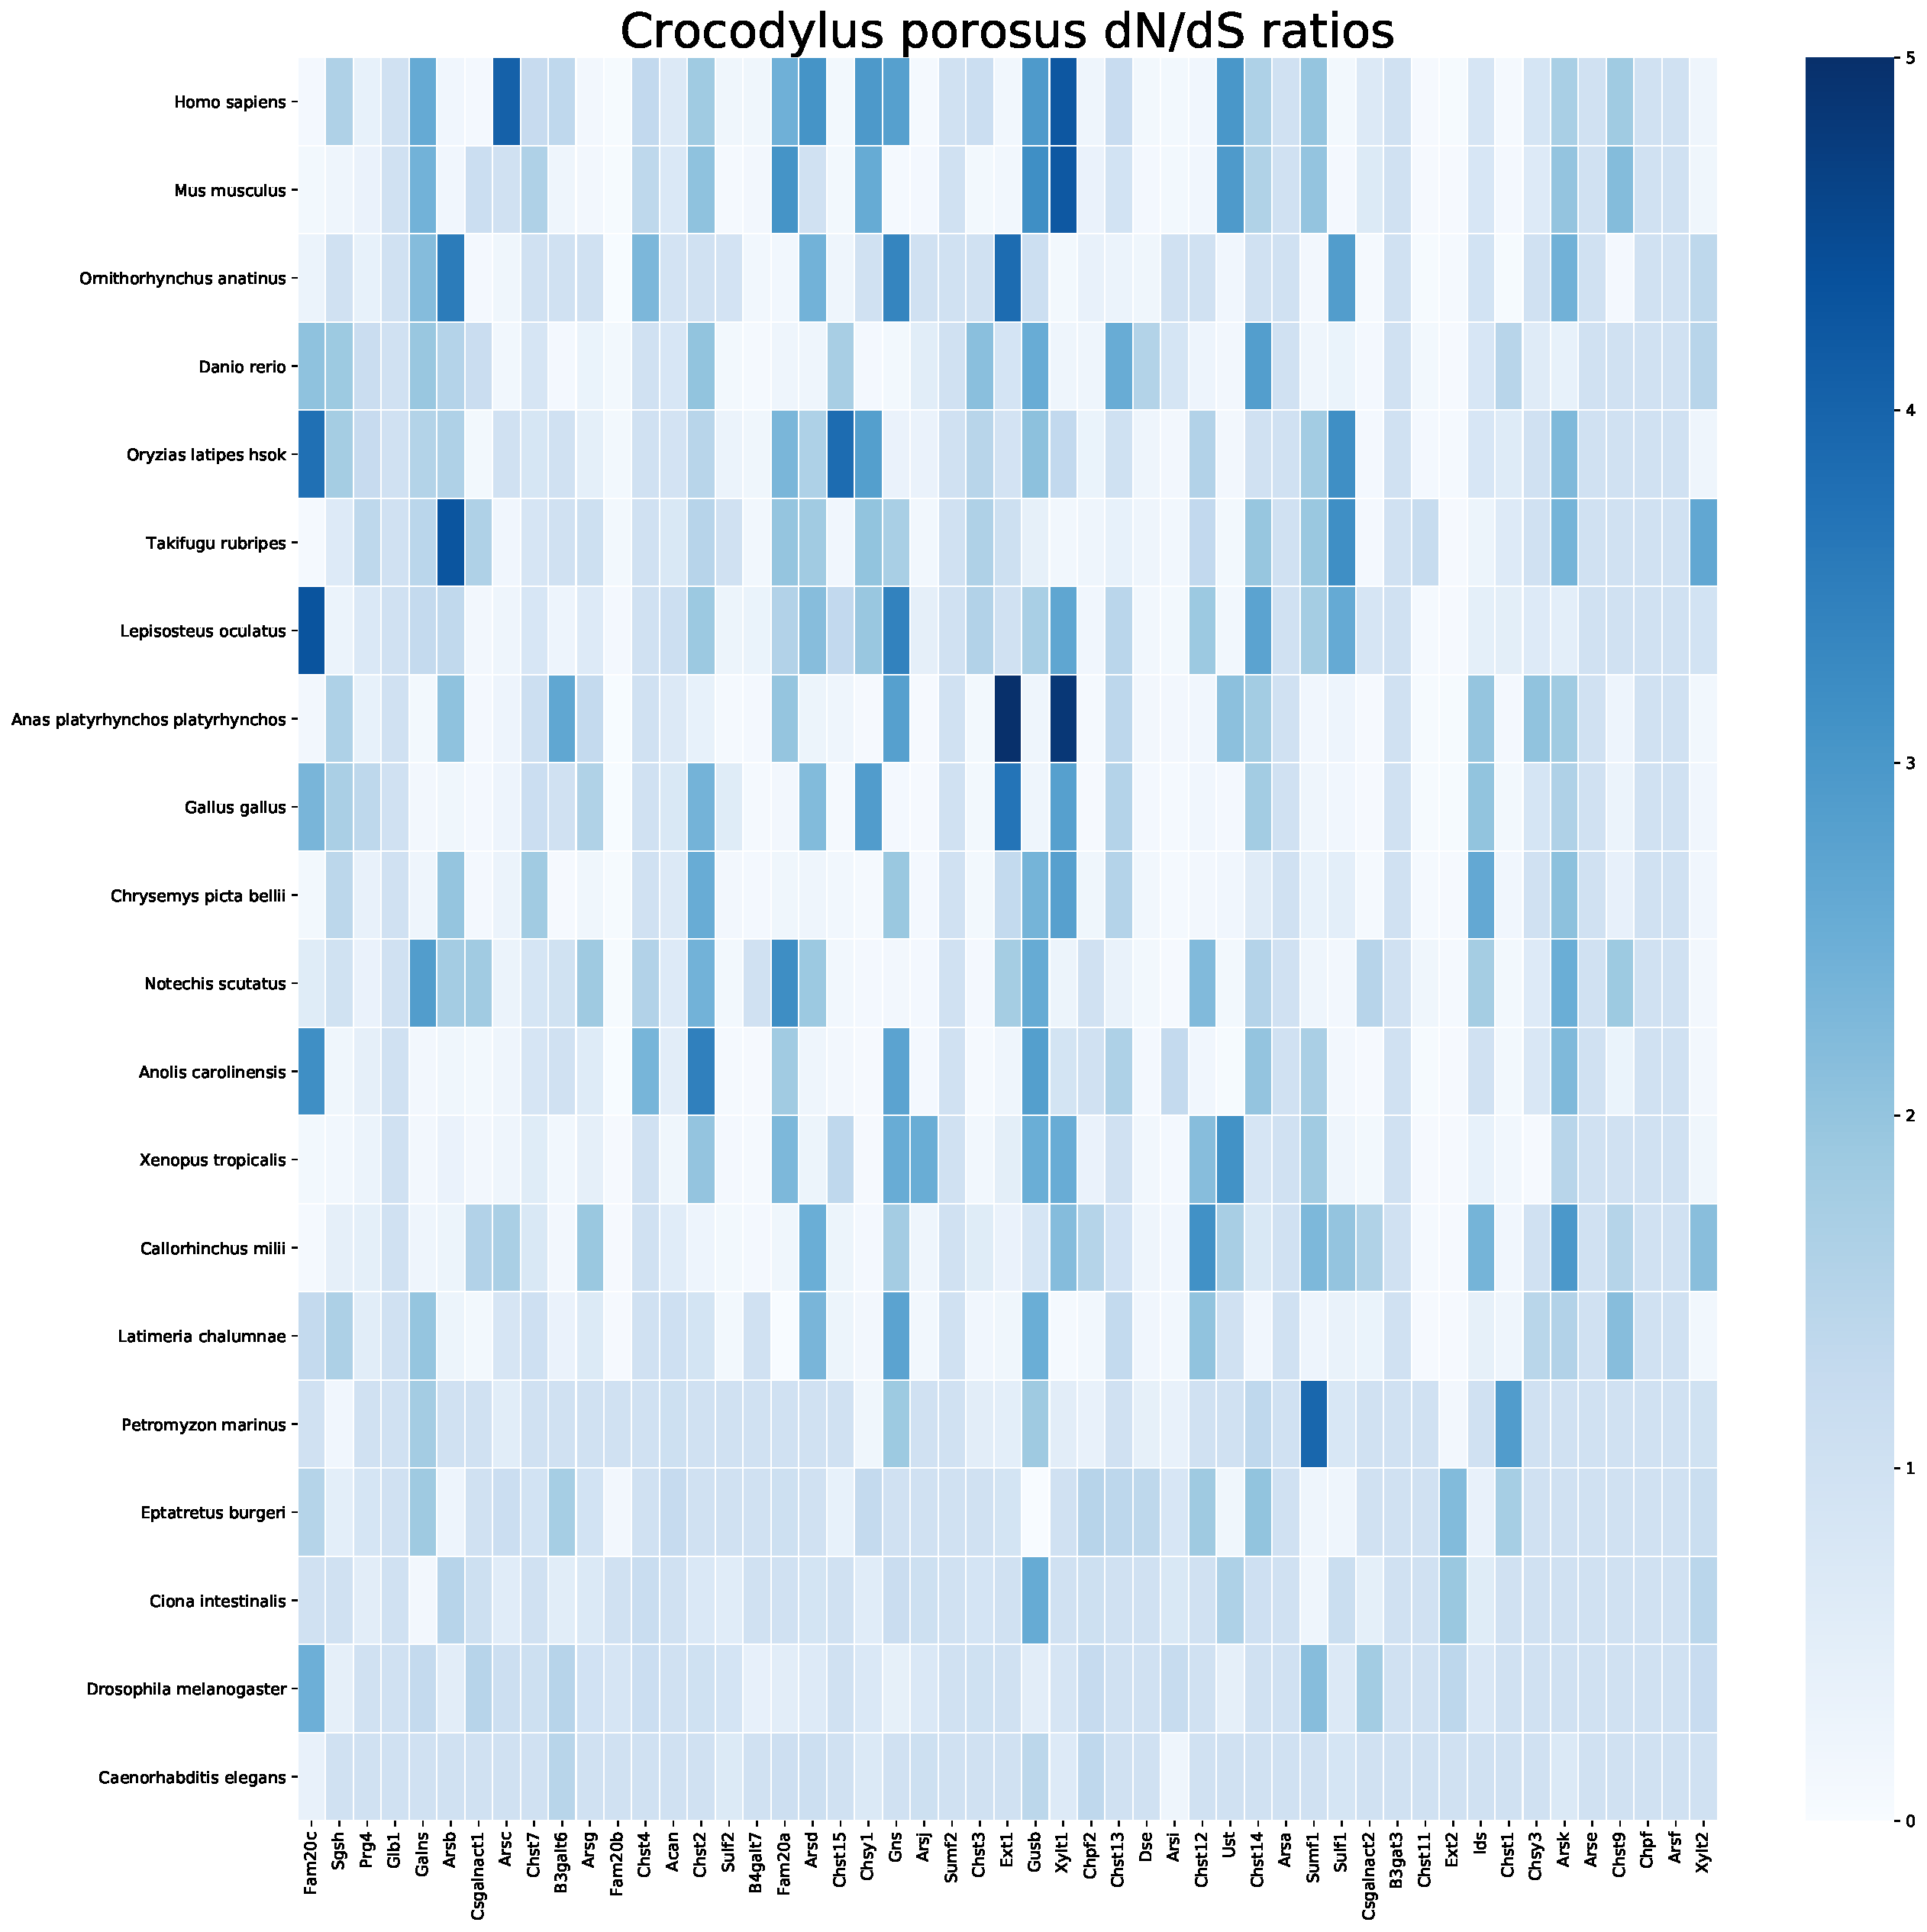
\includegraphics[height=7in,trim={0 0 0 0in},clip]{./appendix_images/dnds/crocodylus_porosus.pdf}}
\caption{\textbf{dN/dS 2D grid for \textit{Crocodylus porosus} computed against the other significant organisms.} The intensity values represent the dN/dS ratio - values lighter in colour are less than 1 and purifying selection while values darker in colour are greater than 1 and represent positive selection.}
\label{sup_fig_22}
\end{figure}

\begin{figure}[H]
\centering
\makebox[\textwidth][c]{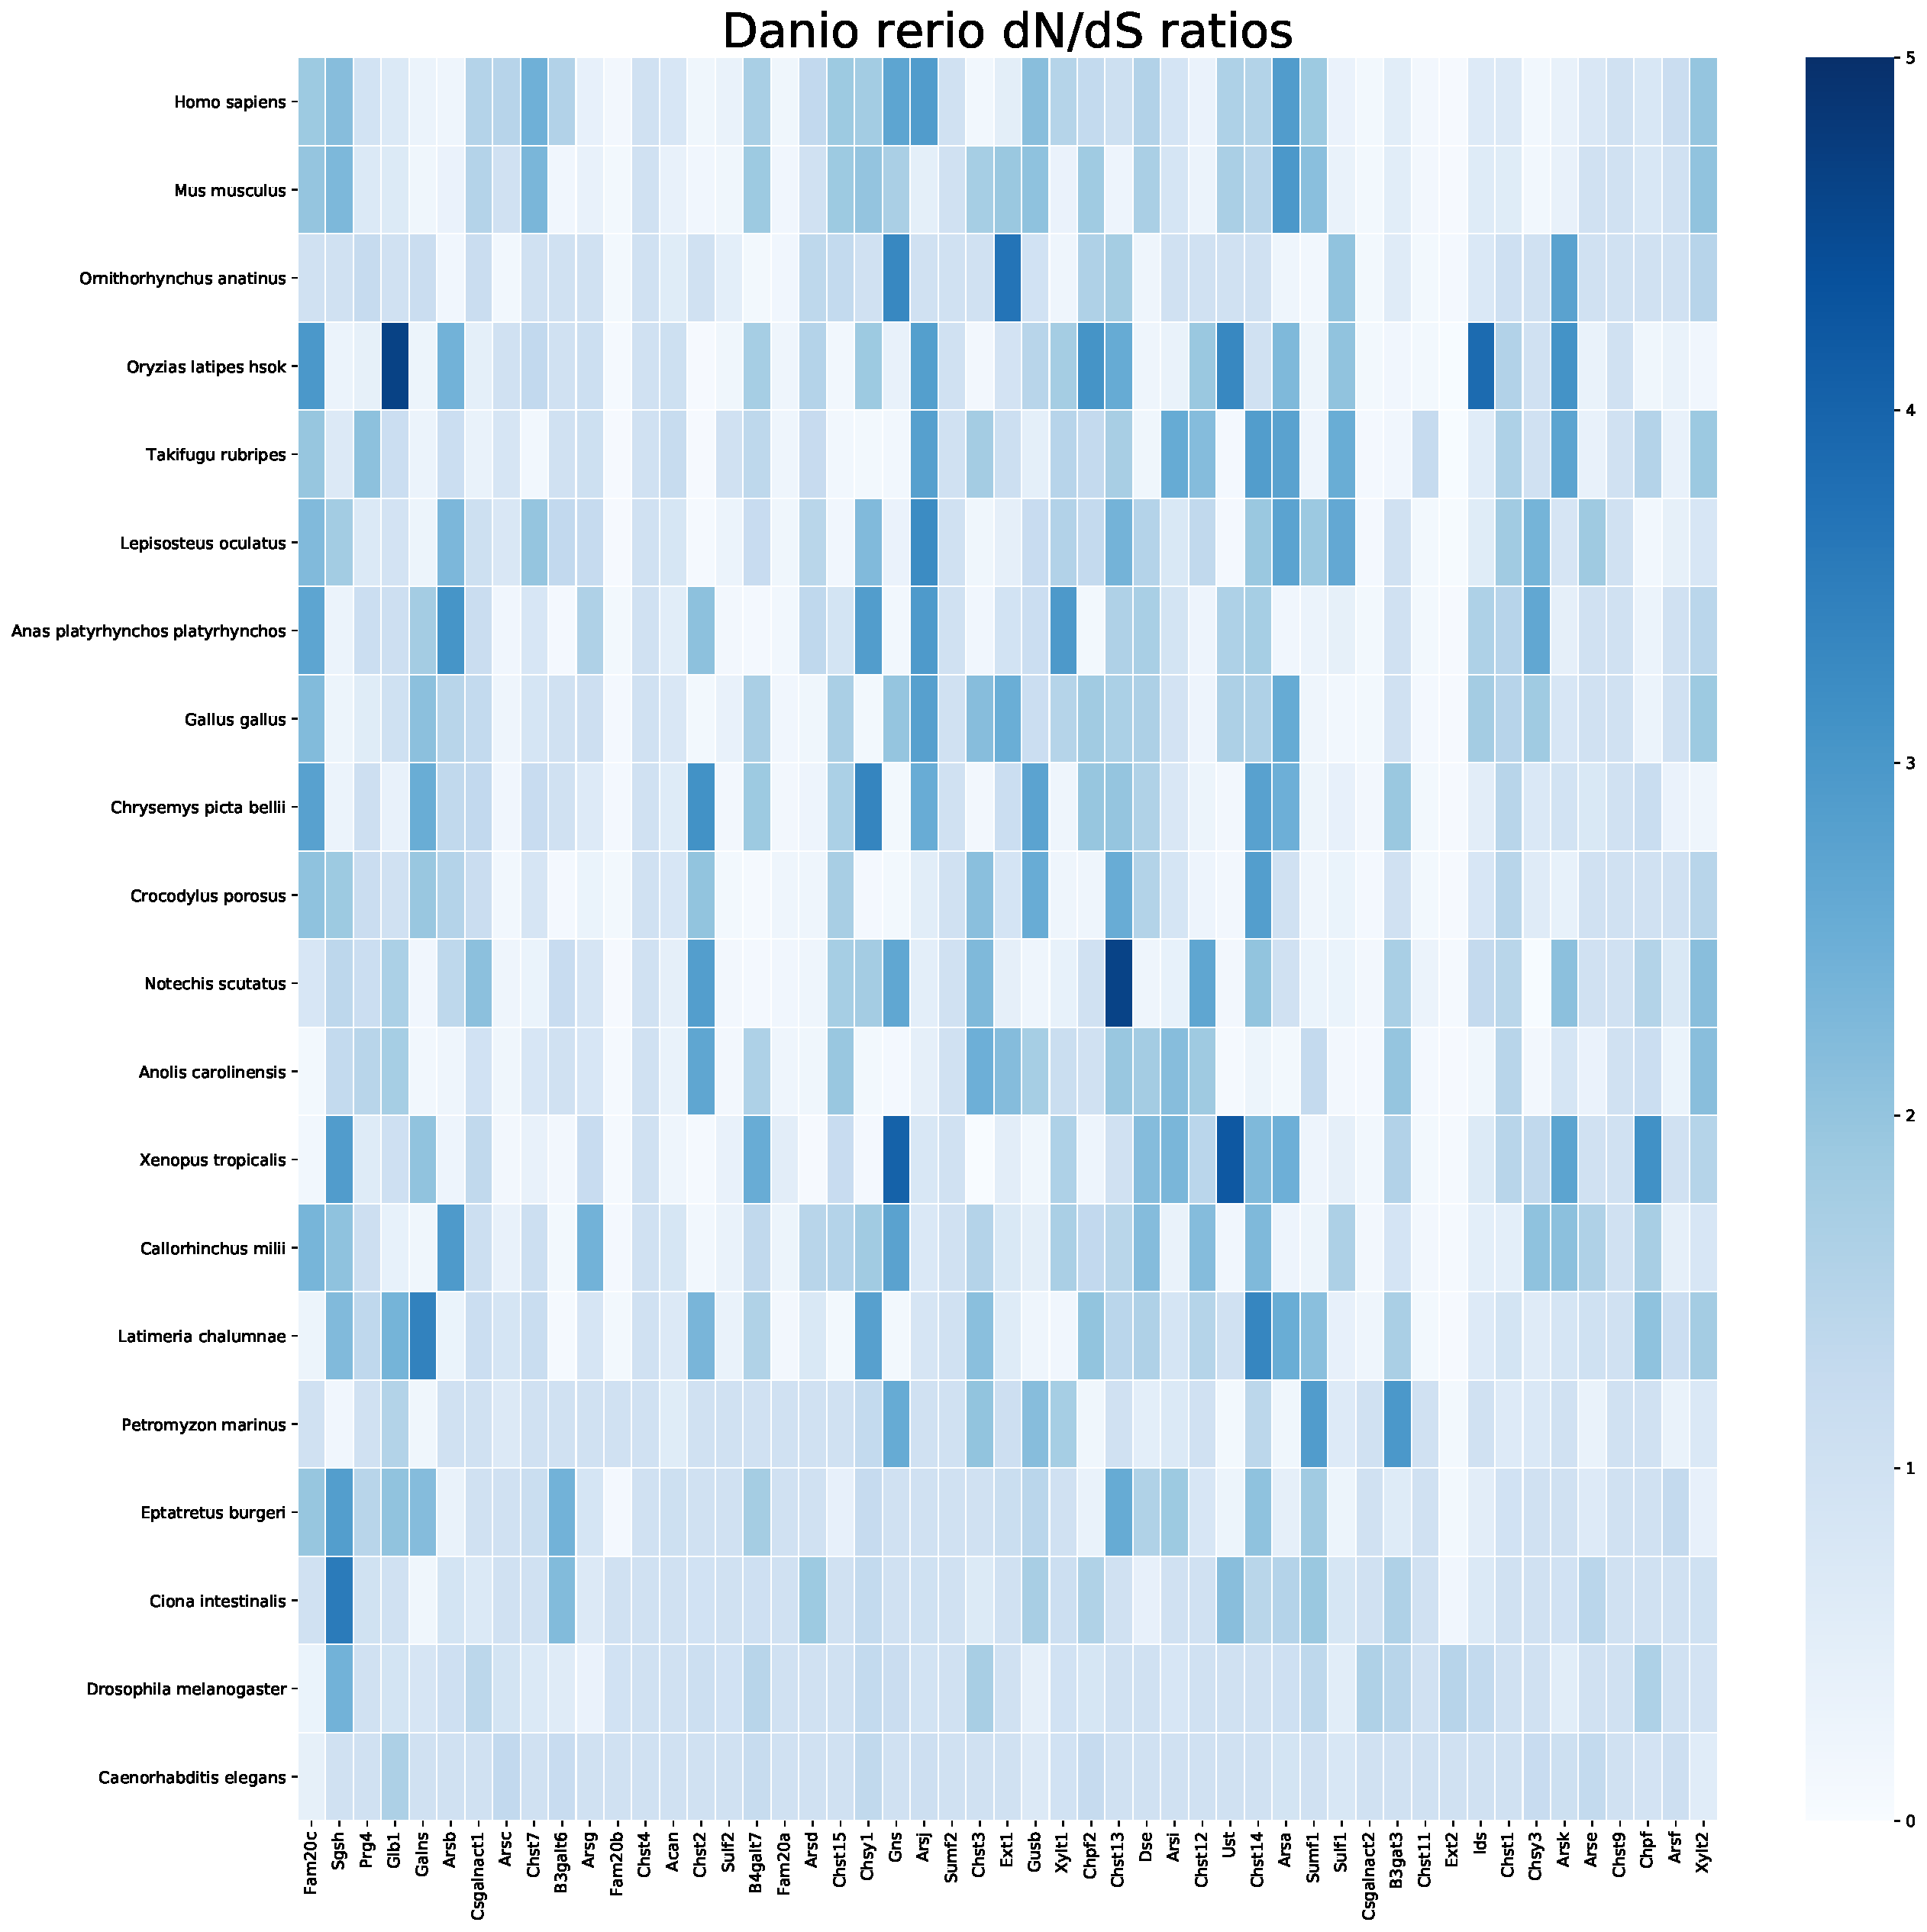
\includegraphics[height=7in,trim={0 0 0 0in},clip]{./appendix_images/dnds/danio_rerio.pdf}}
\caption{\textbf{dN/dS 2D grid for \textit{Danio rerio} computed against the other significant organisms.} The intensity values represent the dN/dS ratio - values lighter in colour are less than 1 and purifying selection while values darker in colour are greater than 1 and represent positive selection.}
\label{sup_fig_23}
\end{figure}

\begin{figure}[H]
\centering
\makebox[\textwidth][c]{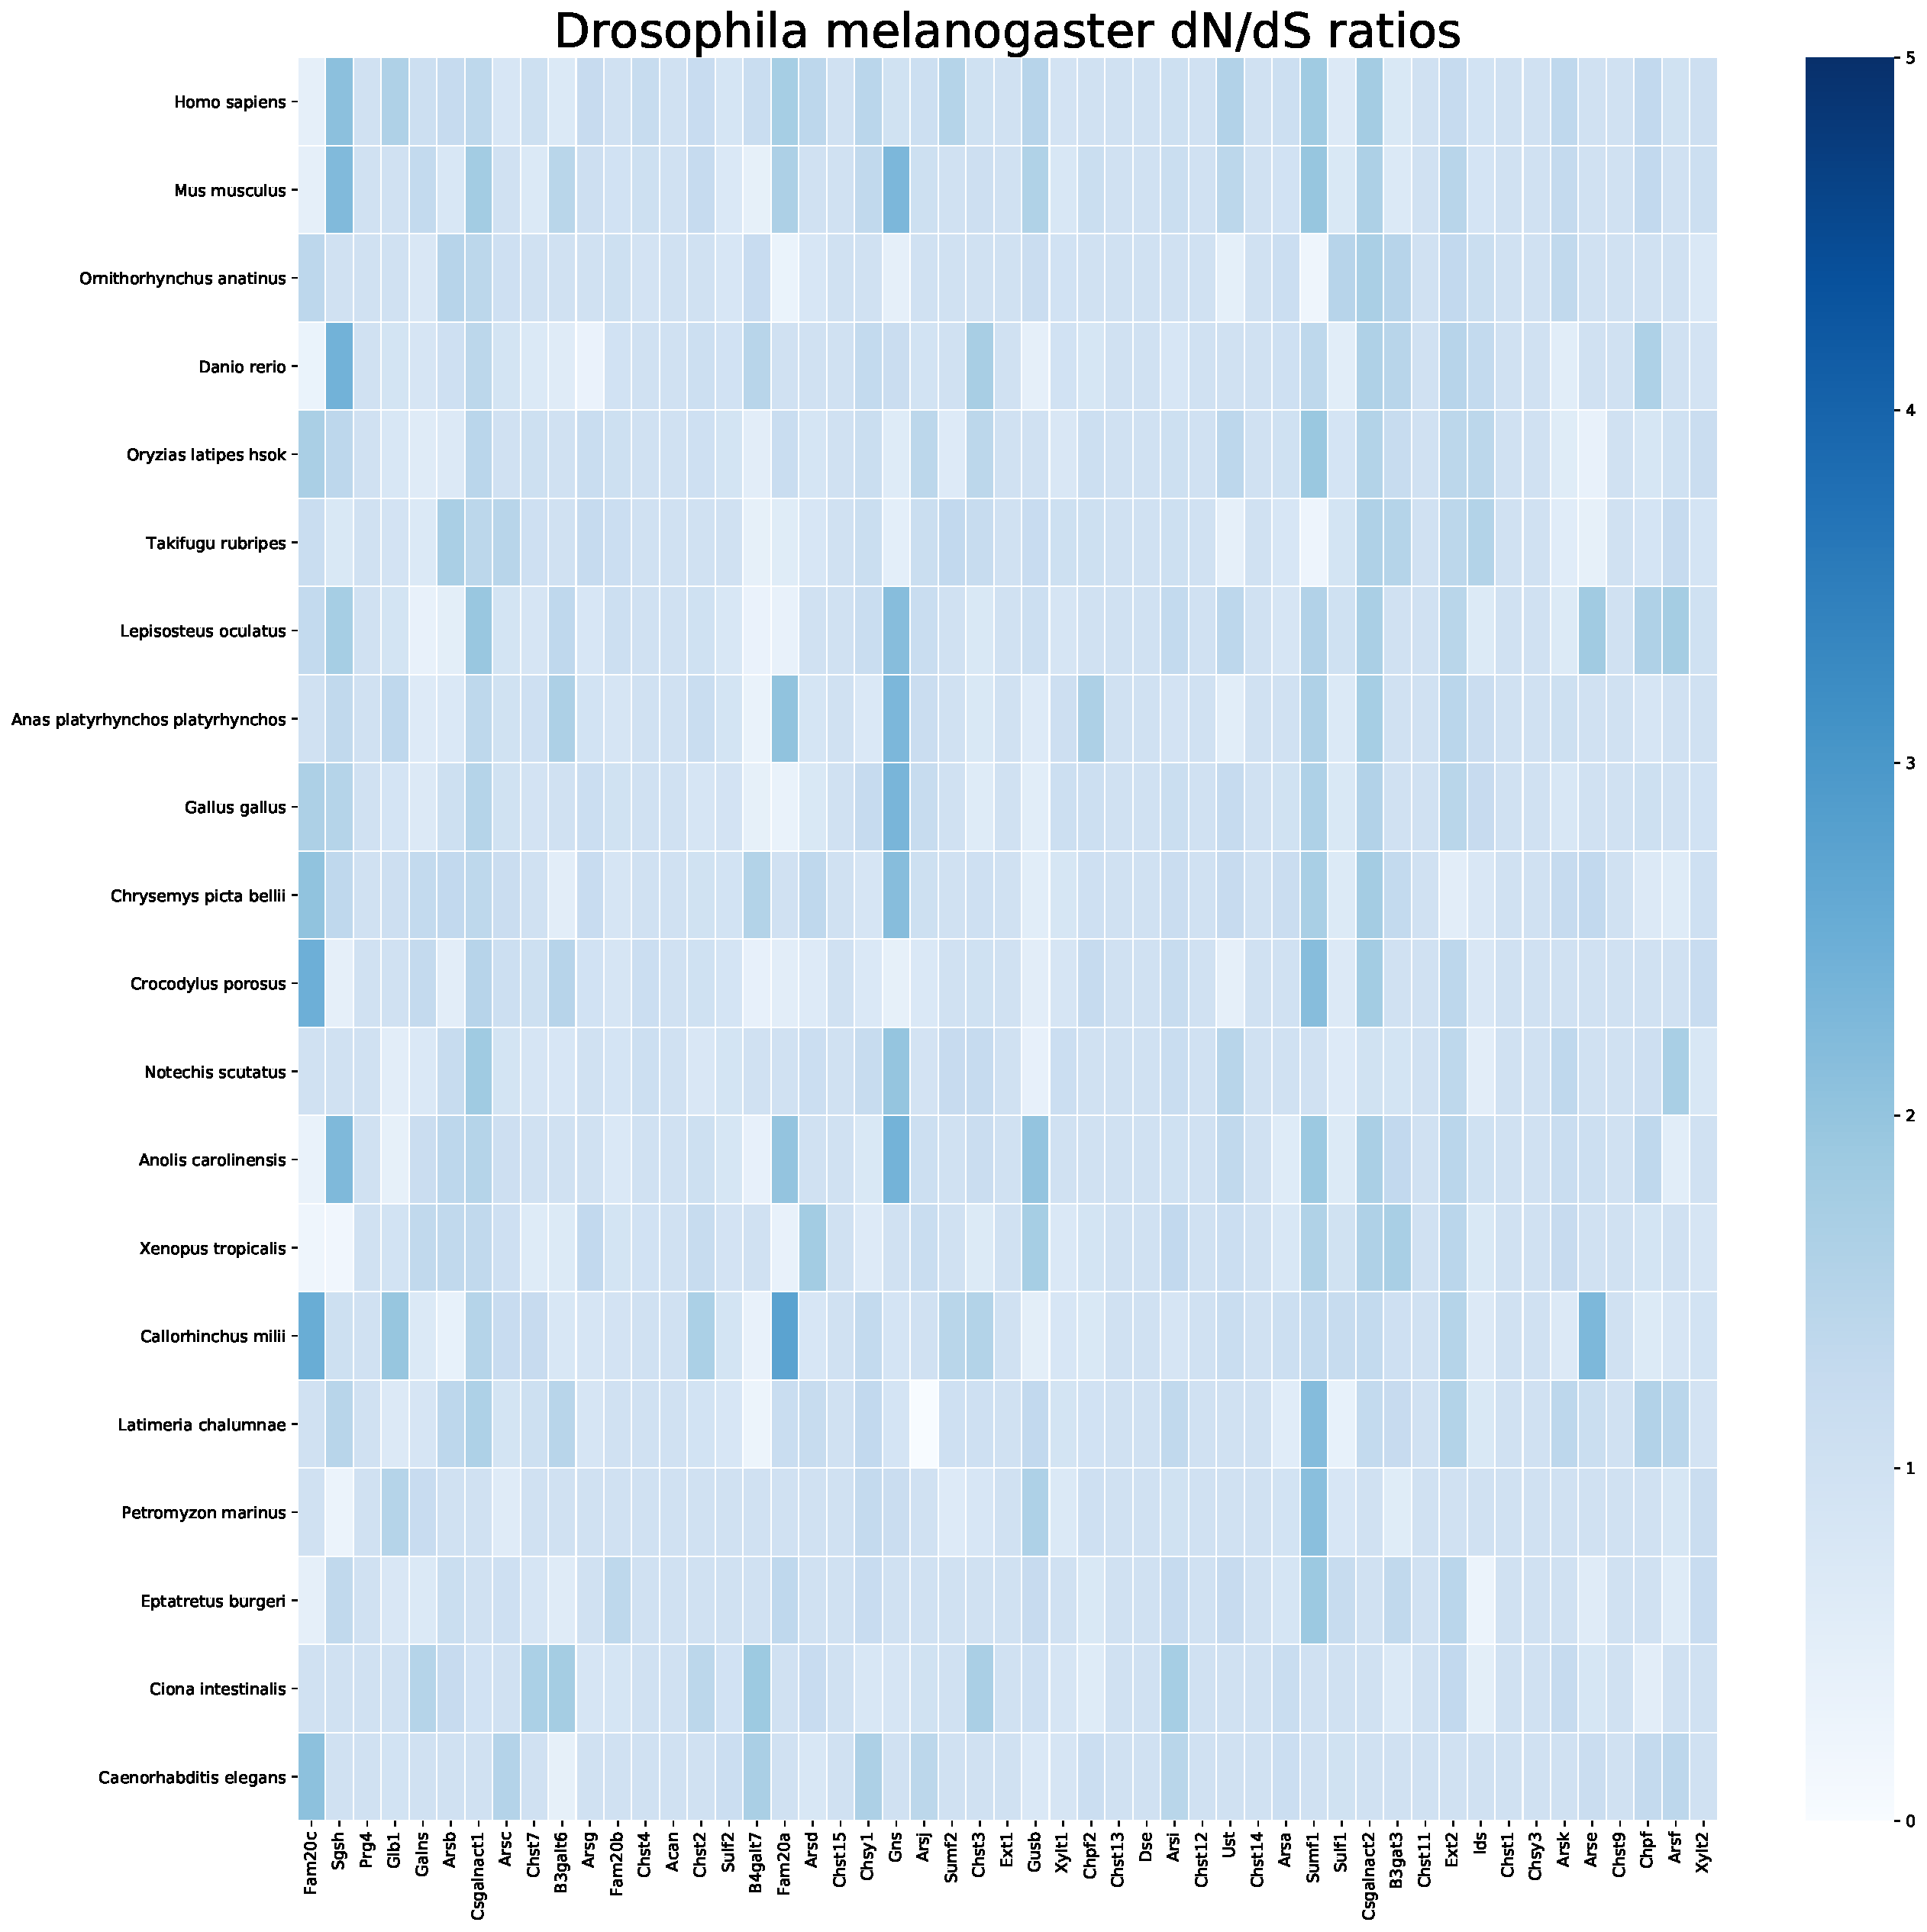
\includegraphics[height=7in,trim={0 0 0 0in},clip]{./appendix_images/dnds/drosophila_melanogaster.pdf}}
\caption{\textbf{dN/dS 2D grid for \textit{Drosophila melanogaster} computed against the other significant organisms.} The intensity values represent the dN/dS ratio - values lighter in colour are less than 1 and purifying selection while values darker in colour are greater than 1 and represent positive selection.}
\label{sup_fig_24}
\end{figure}

\begin{figure}[H]
\centering
\makebox[\textwidth][c]{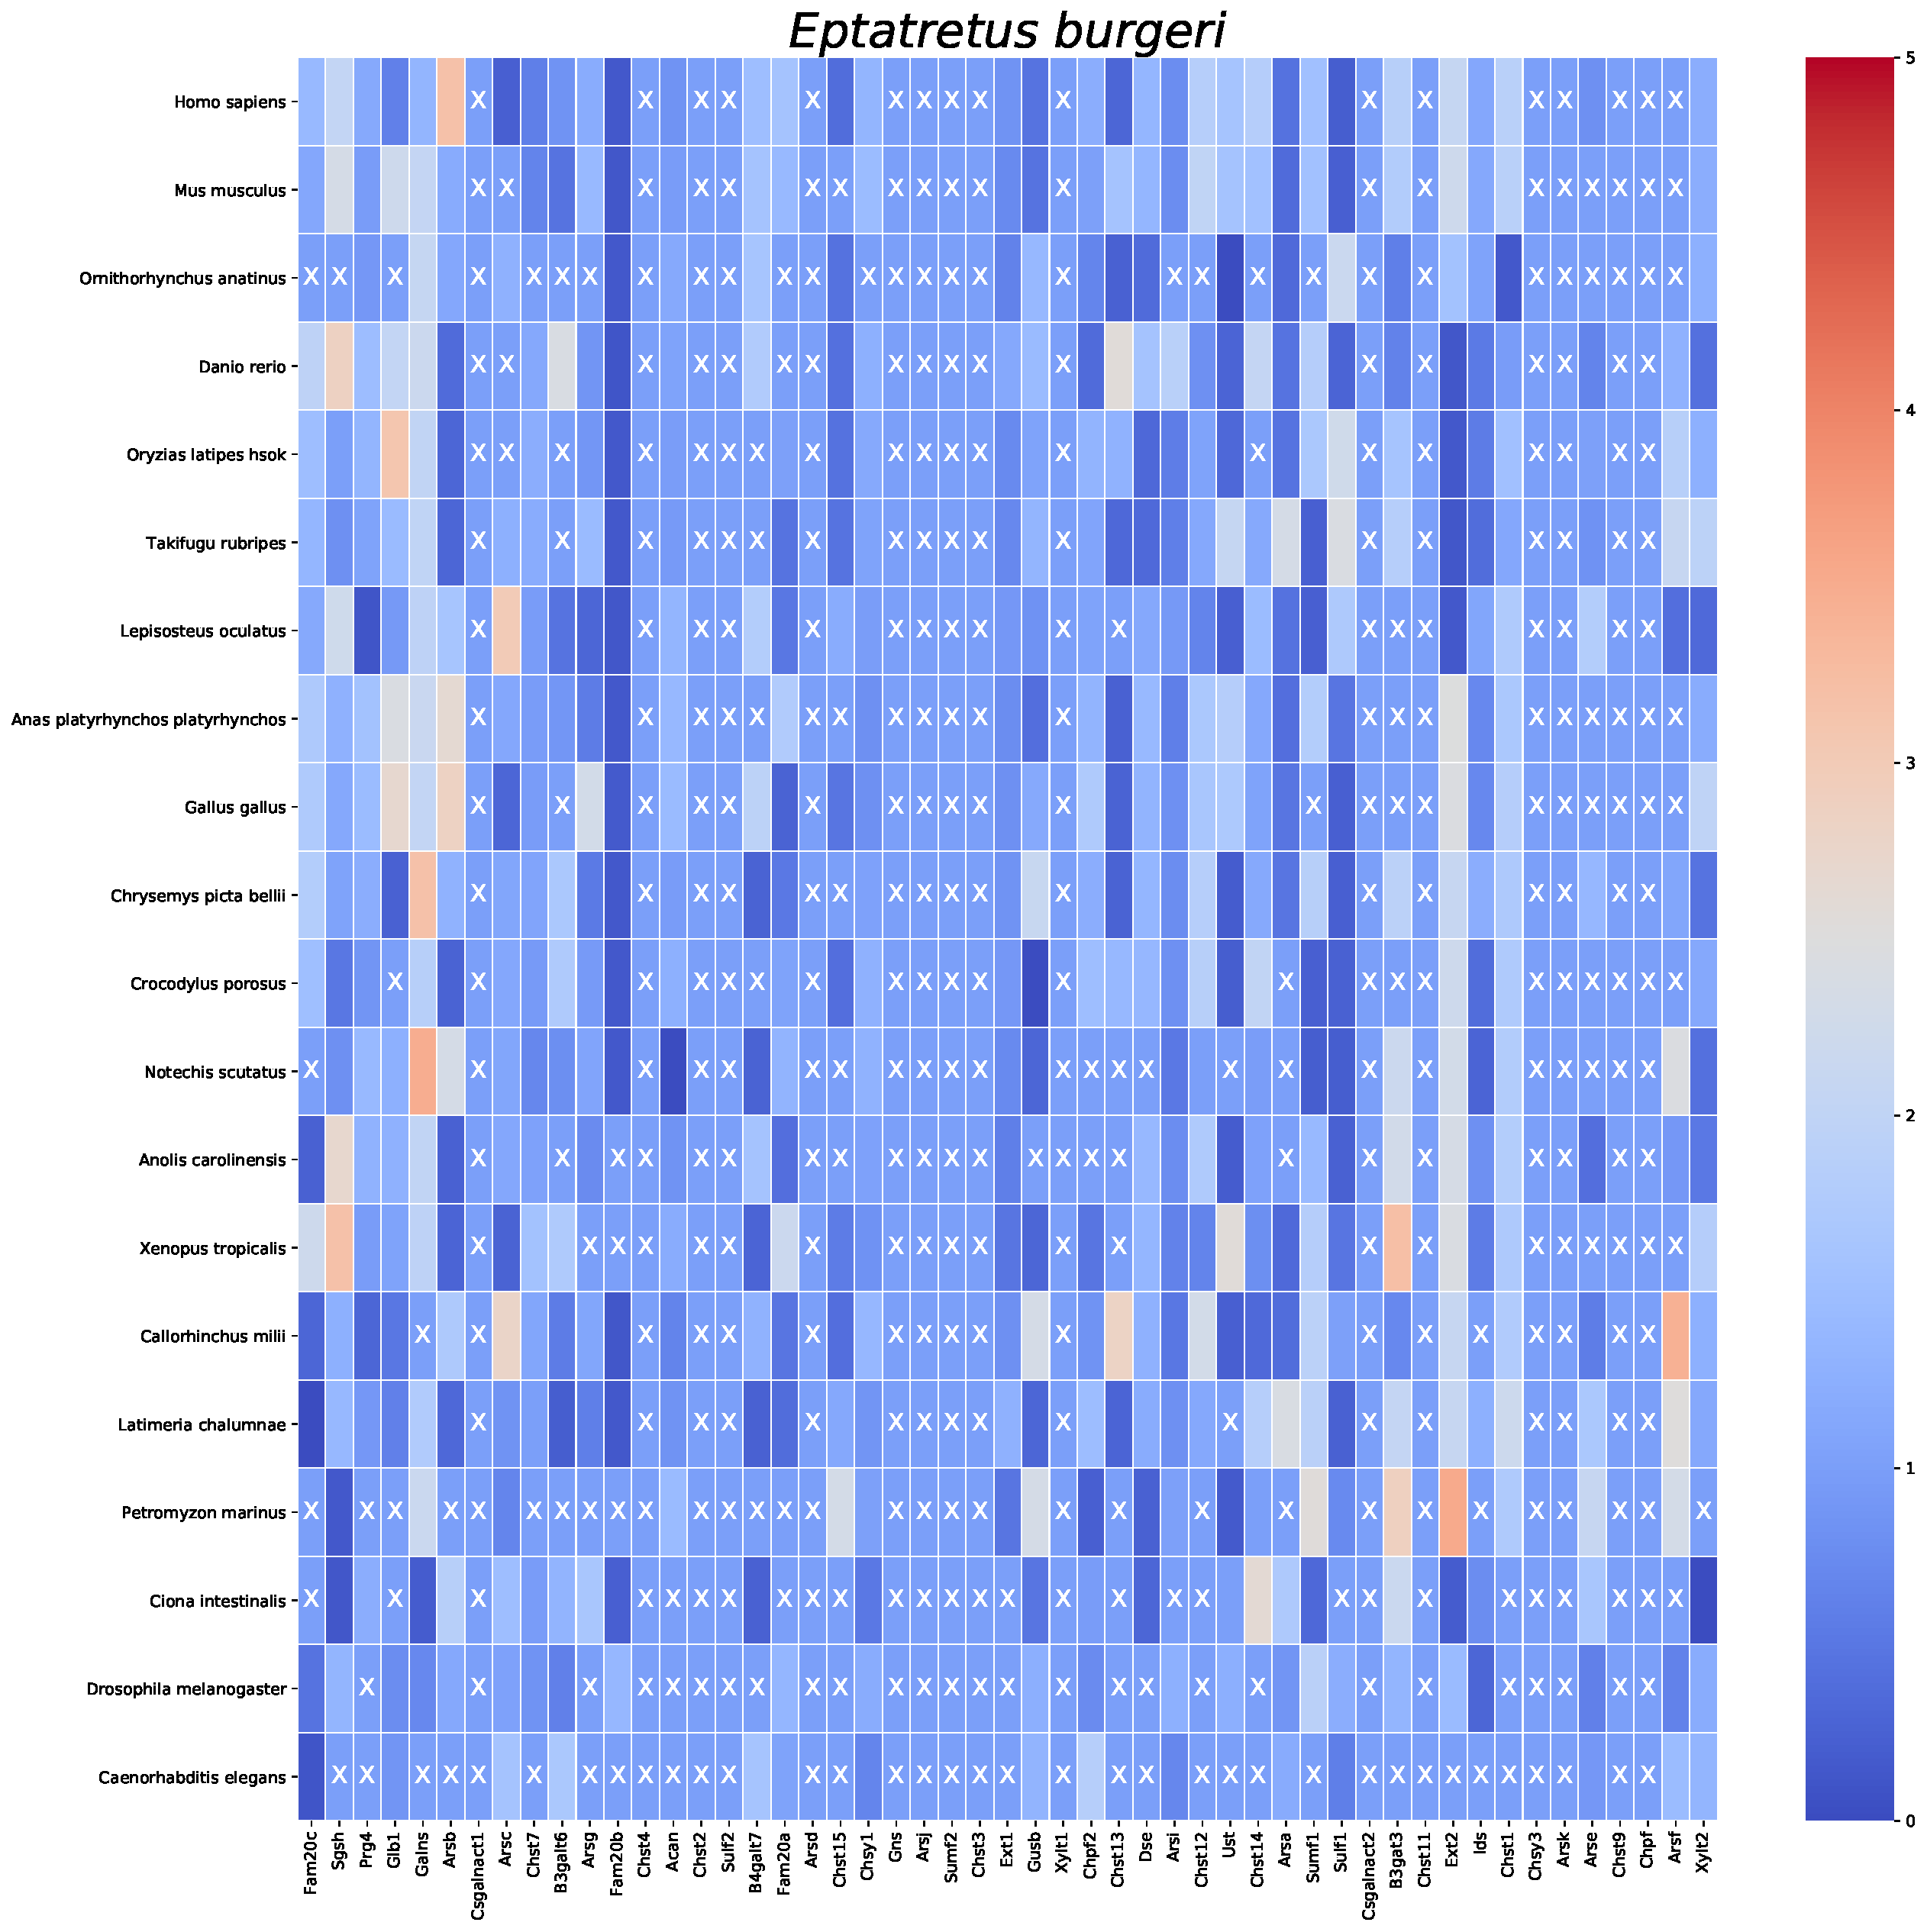
\includegraphics[height=7in,trim={0 0 0 0in},clip]{./appendix_images/dnds/eptatretus_burgeri.pdf}}
\caption{\textbf{dN/dS 2D grid for \textit{Eptatretus burgeri} computed against the other significant organisms.} The intensity values represent the dN/dS ratio - values lighter in colour are less than 1 and purifying selection while values darker in colour are greater than 1 and represent positive selection.}
\label{sup_fig_25}
\end{figure}

\begin{figure}[H]
\centering
\makebox[\textwidth][c]{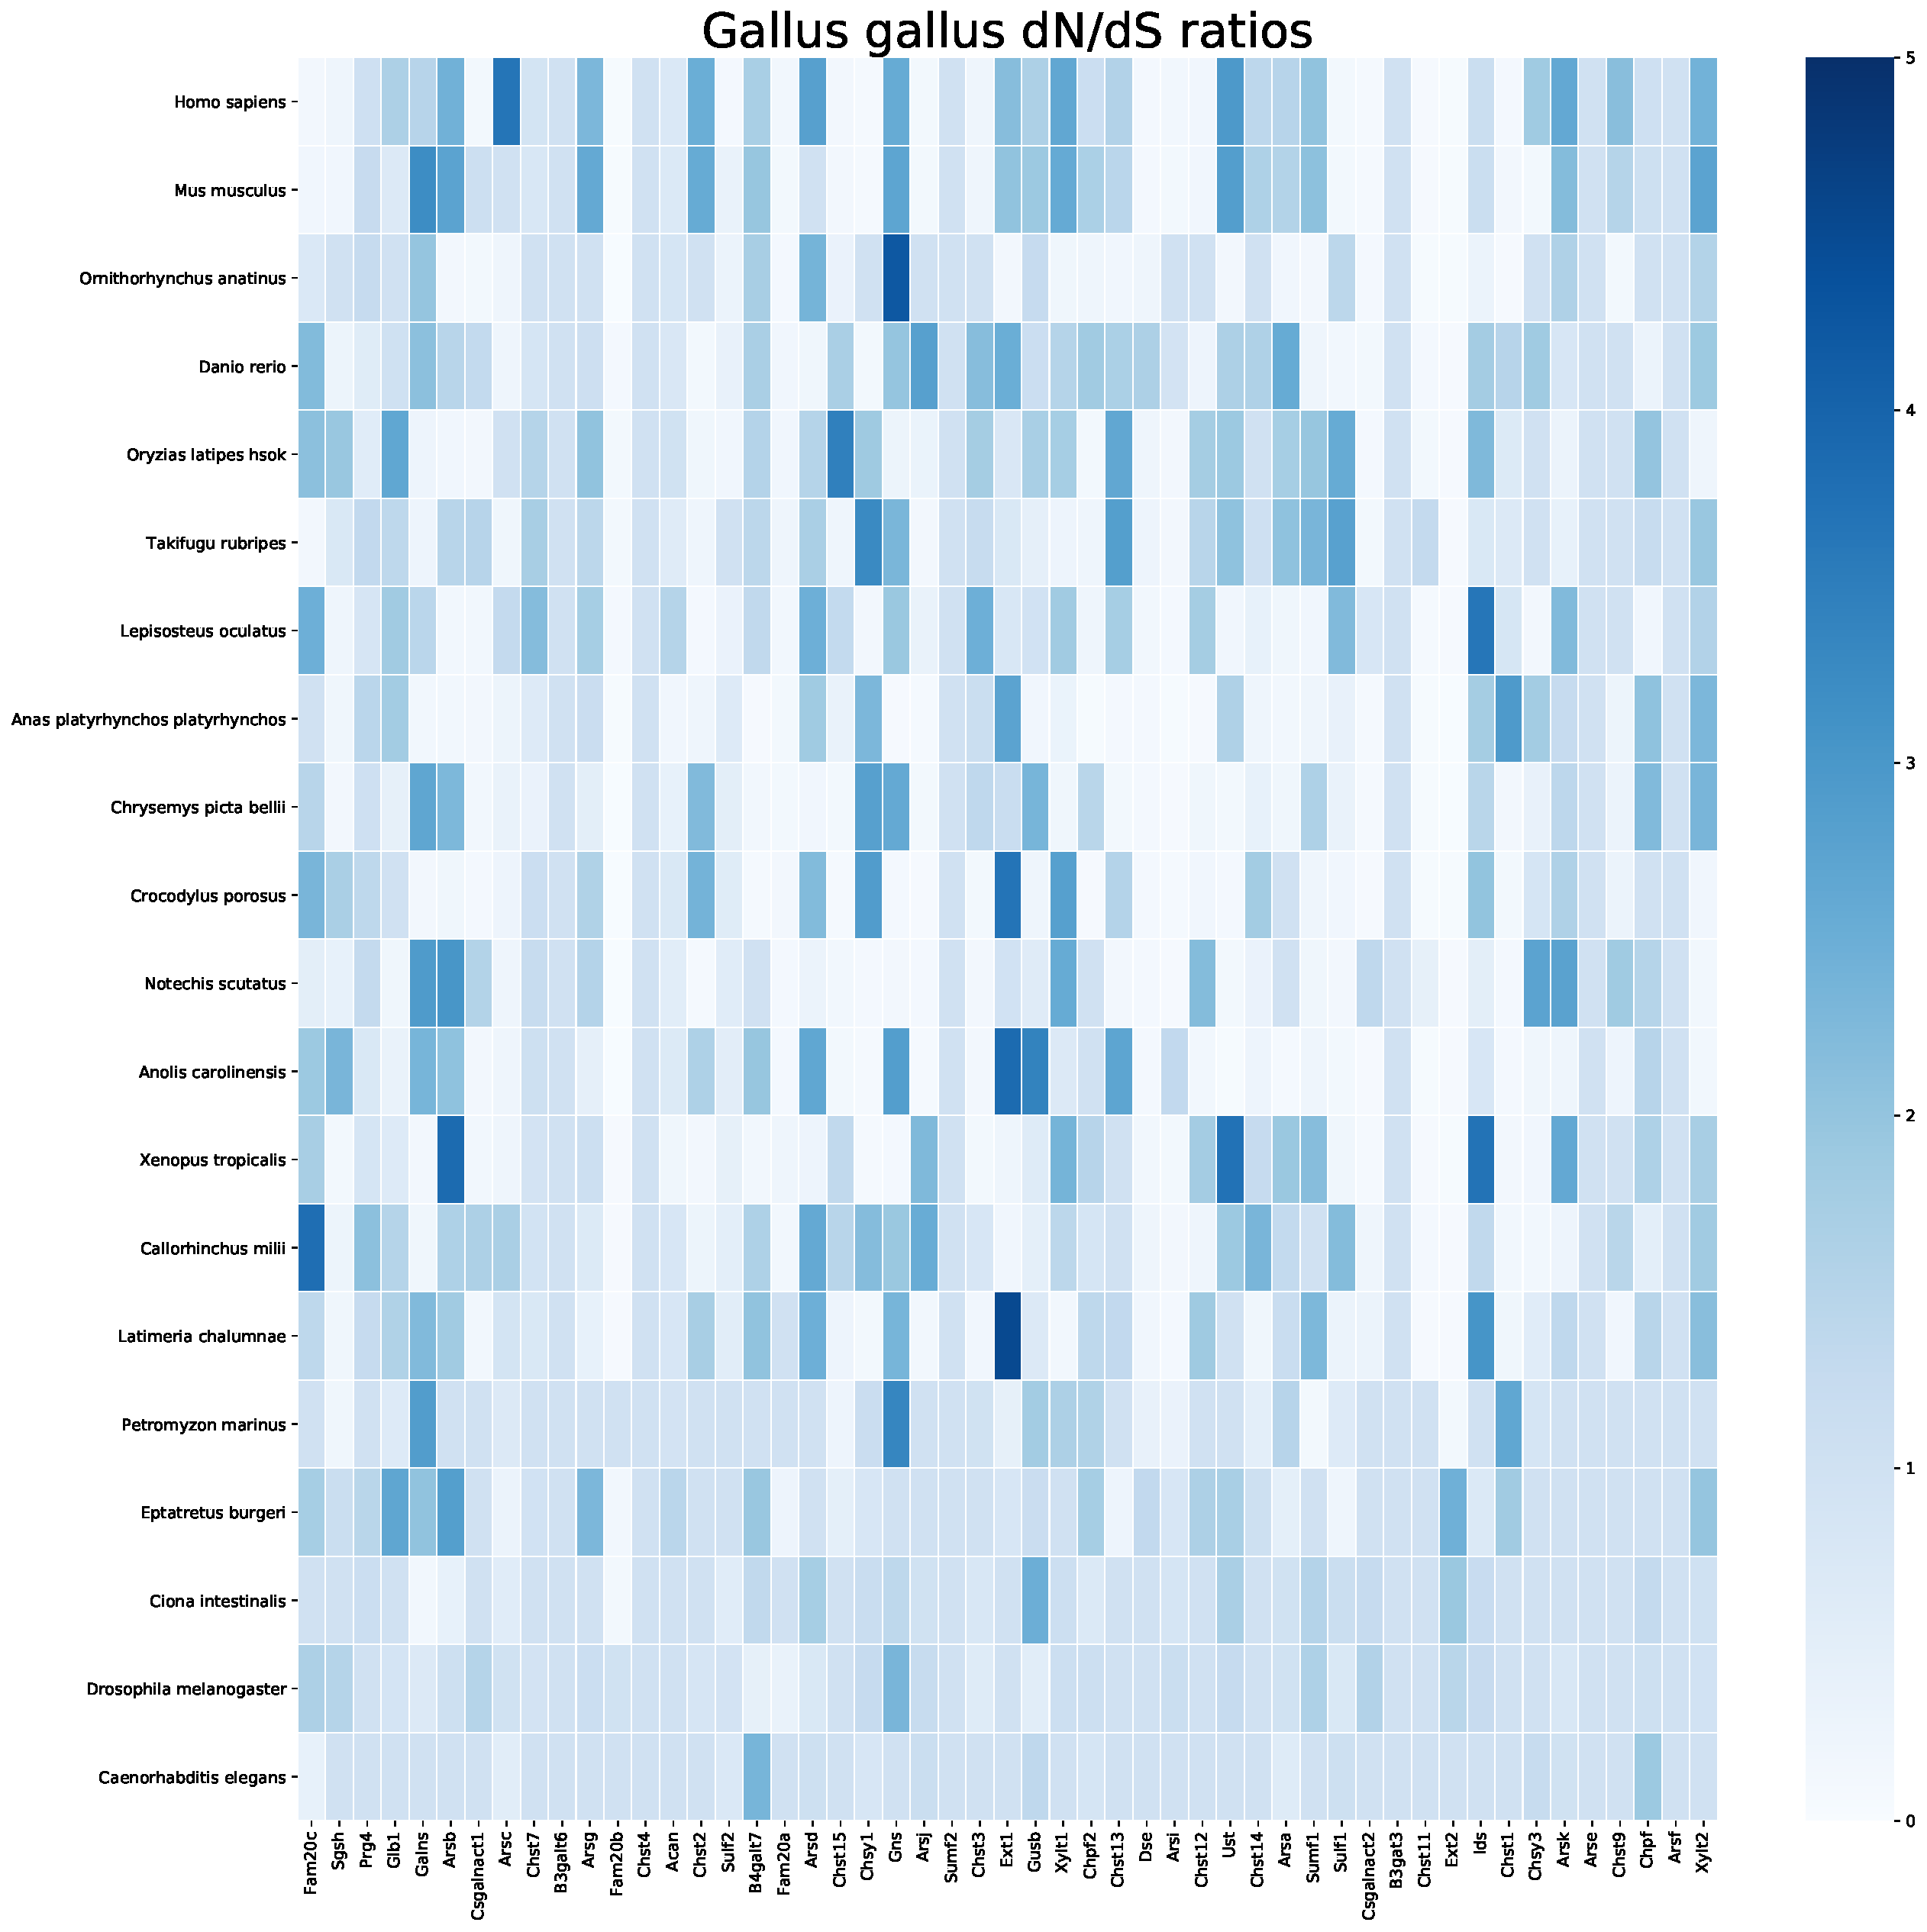
\includegraphics[height=7in,trim={0 0 0 0in},clip]{./appendix_images/dnds/gallus_gallus.pdf}}
\caption{\textbf{dN/dS 2D grid for \textit{Gallus gallus} computed against the other significant organisms.} The intensity values represent the dN/dS ratio - values lighter in colour are less than 1 and purifying selection while values darker in colour are greater than 1 and represent positive selection.}
\label{sup_fig_26}
\end{figure}

\begin{figure}[H]
\centering
\makebox[\textwidth][c]{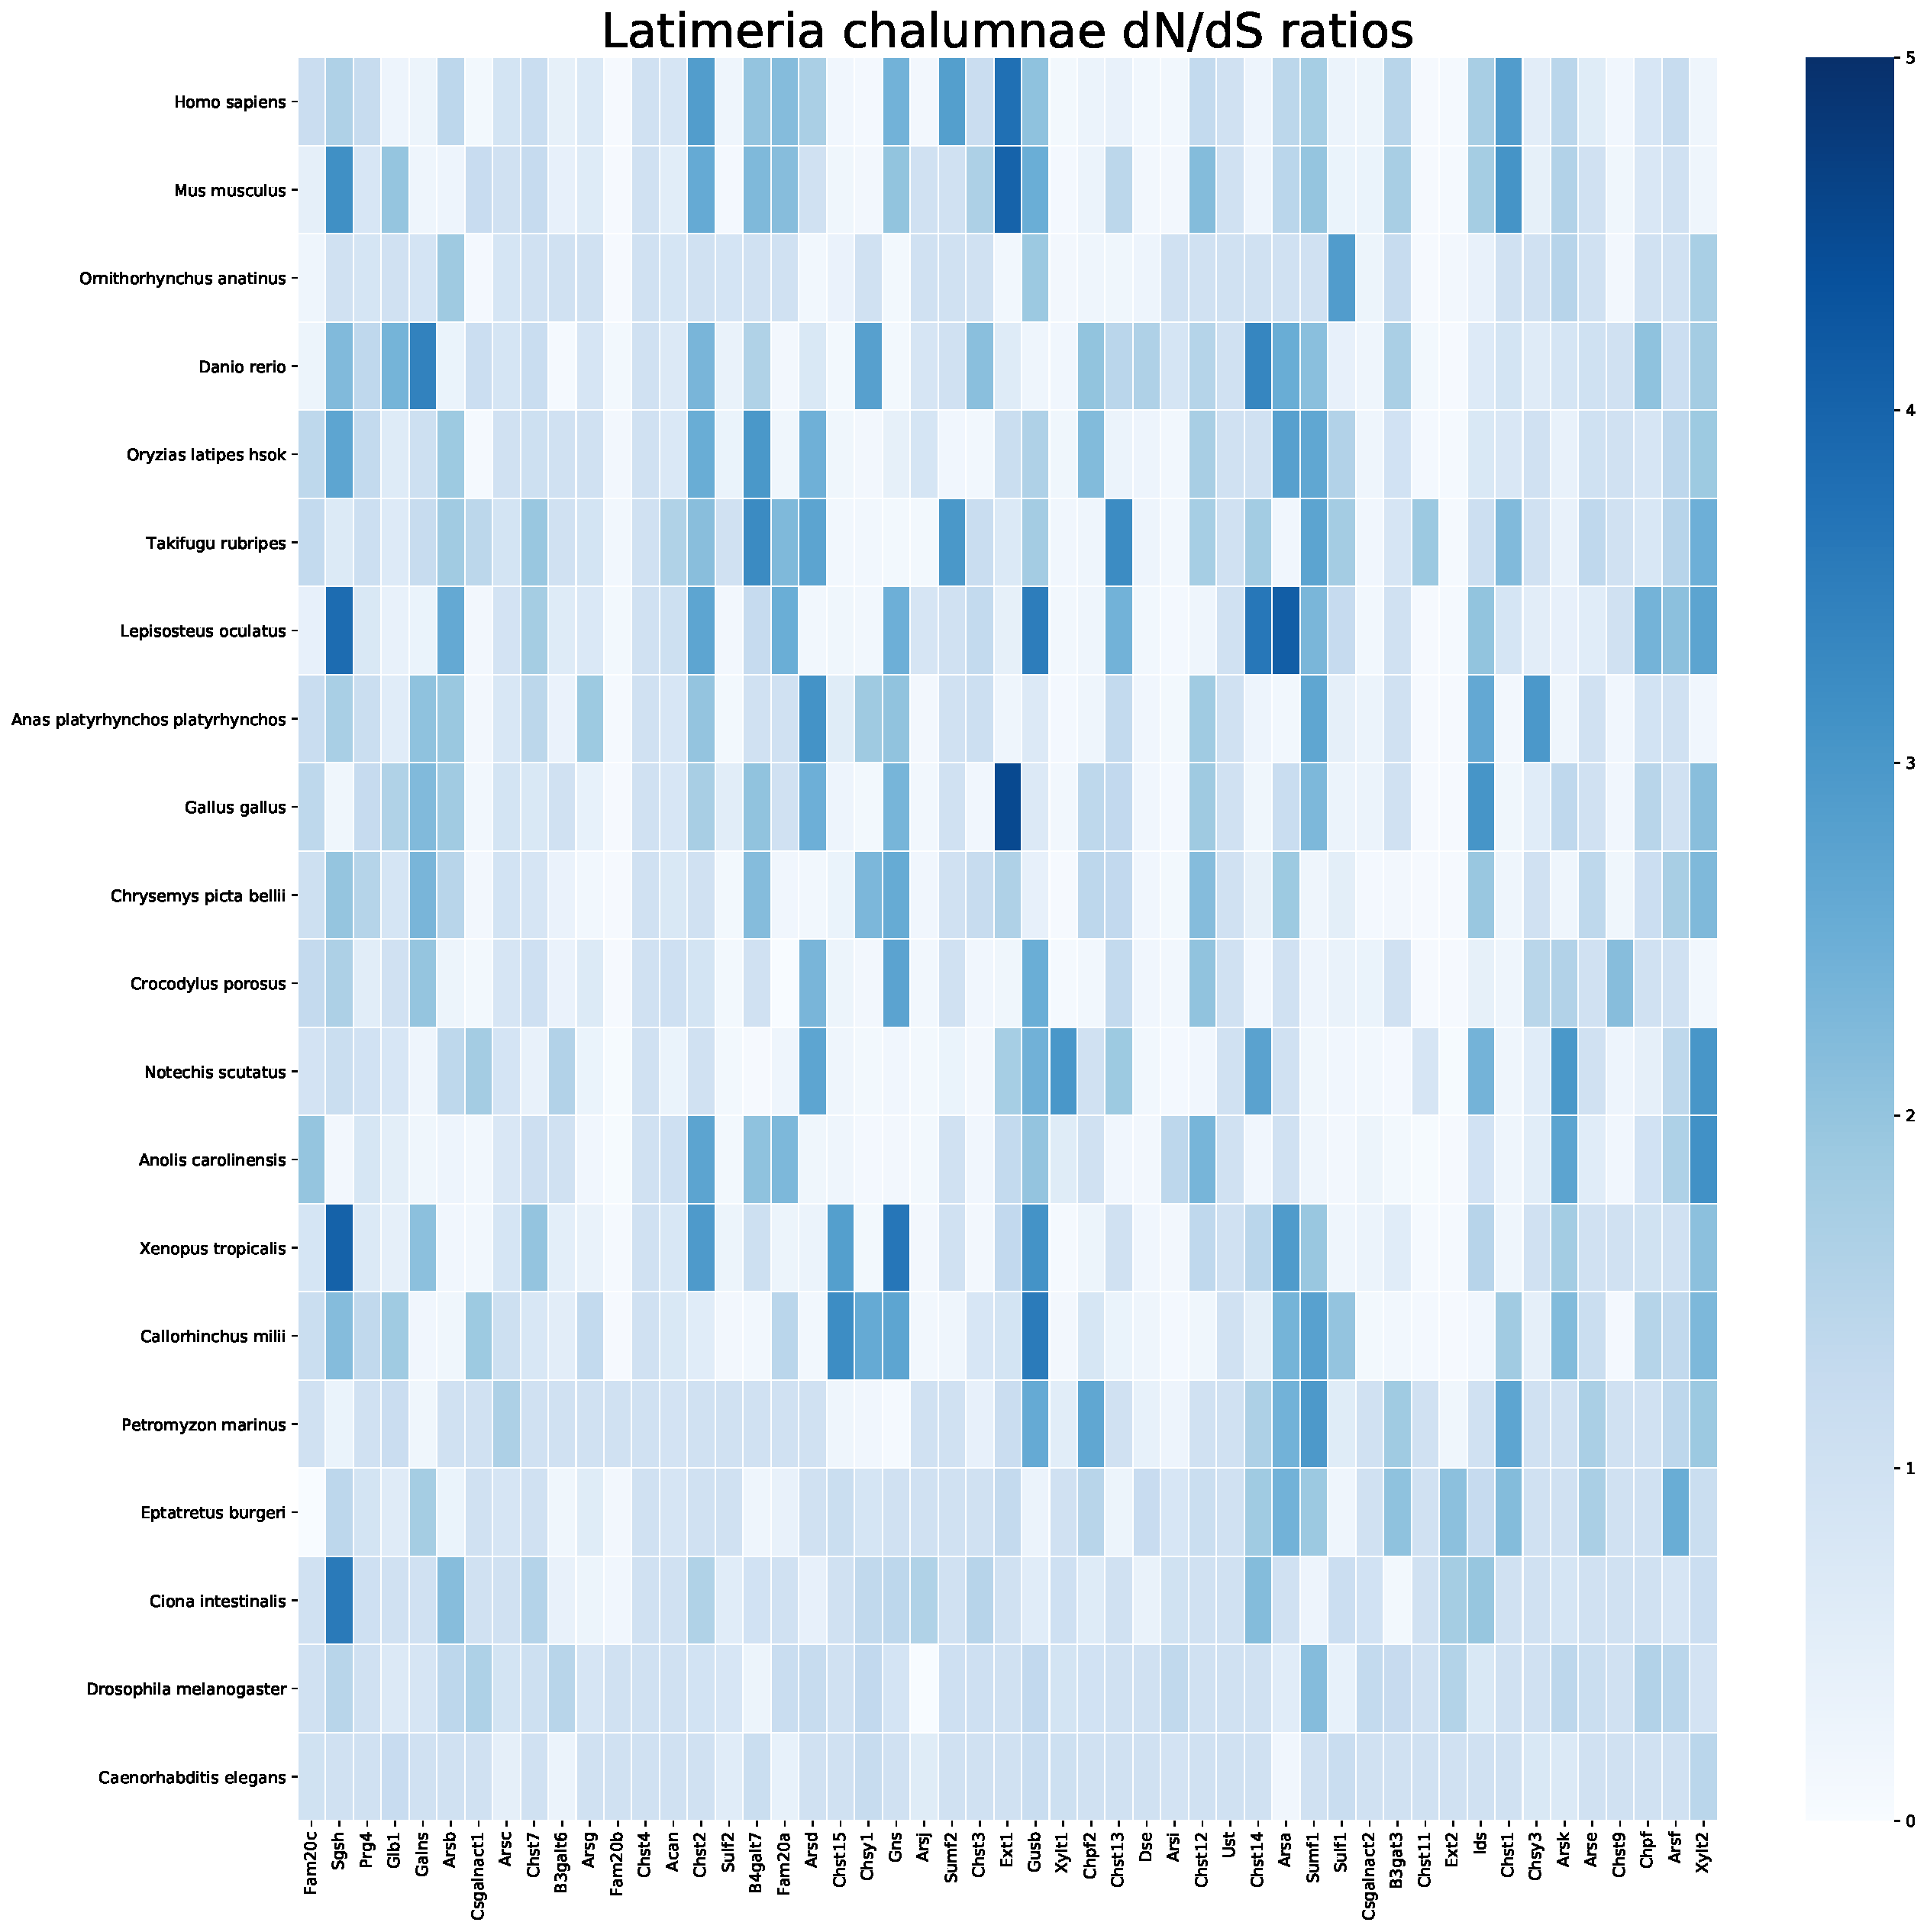
\includegraphics[height=7in,trim={0 0 0 0in},clip]{./appendix_images/dnds/latimeria_chalumnae.pdf}}
\caption{\textbf{dN/dS 2D grid for \textit{Latimeria chalumnae} computed against the other significant organisms.} The intensity values represent the dN/dS ratio - values lighter in colour are less than 1 and purifying selection while values darker in colour are greater than 1 and represent positive selection.}
\label{sup_fig_27}
\end{figure}

\begin{figure}[H]
\centering
\makebox[\textwidth][c]{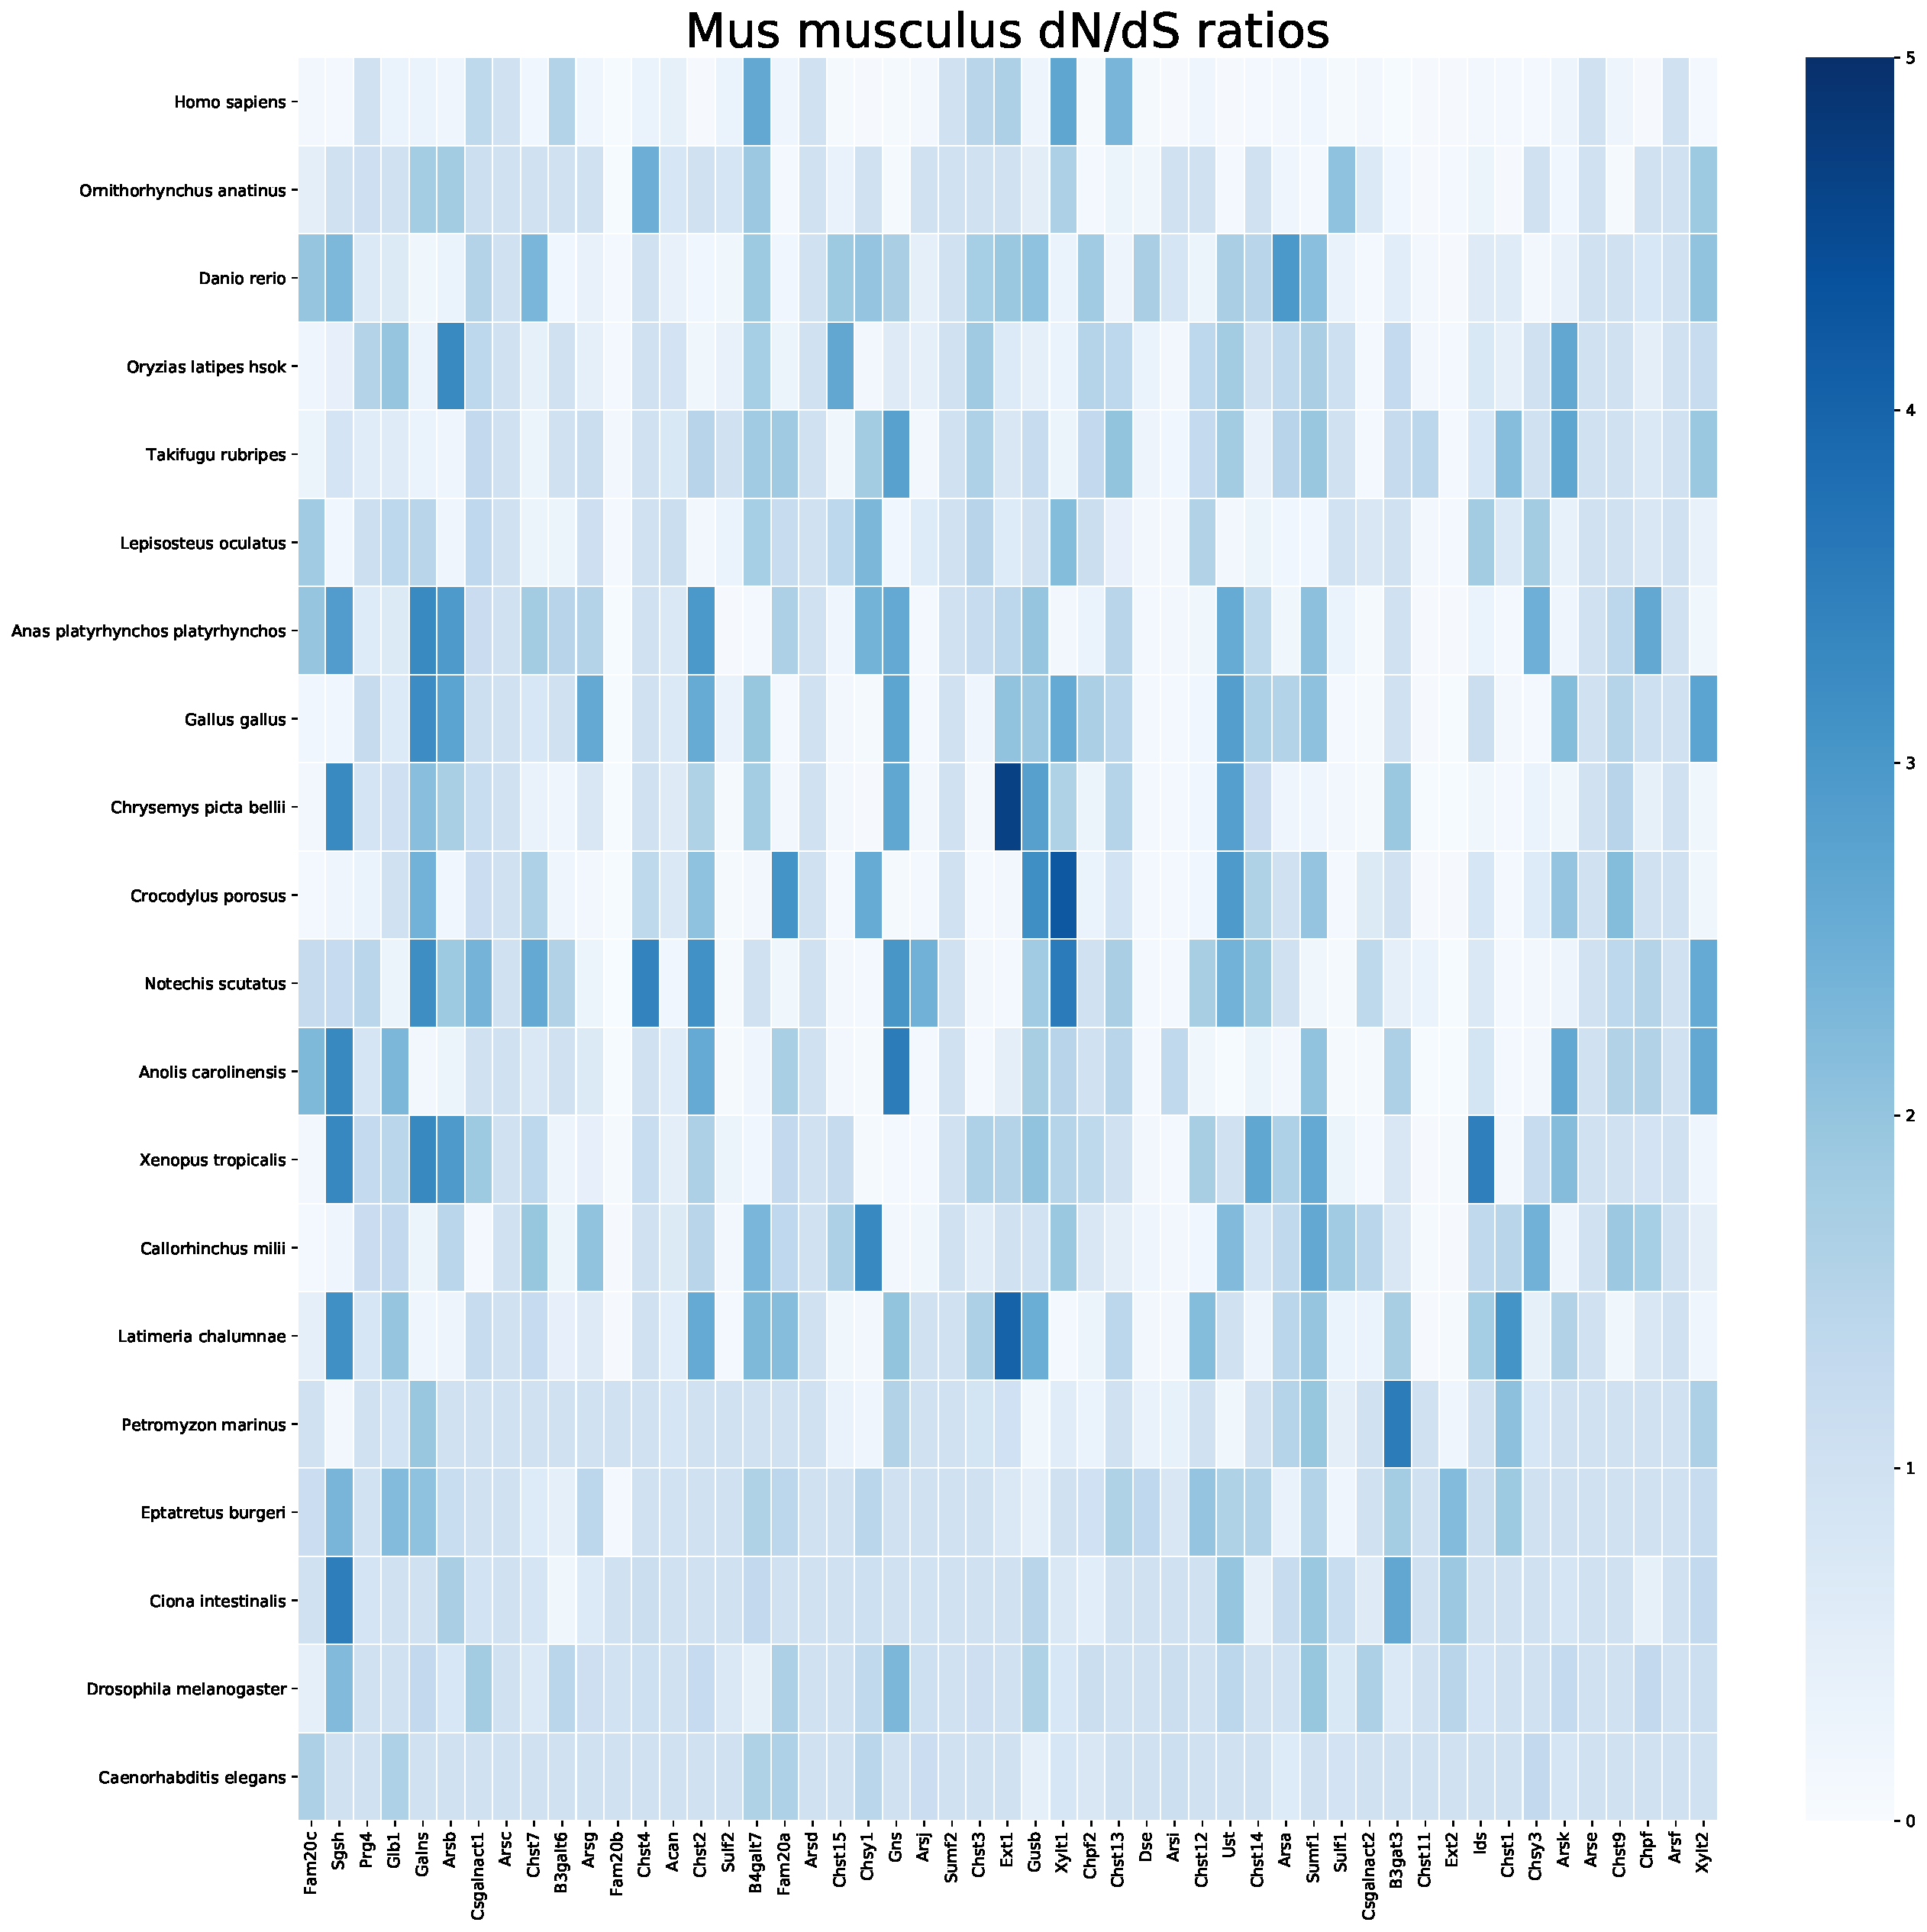
\includegraphics[height=7in,trim={0 0 0 0in},clip]{./appendix_images/dnds/mus_musculus.pdf}}
\caption{\textbf{dN/dS 2D grid for \textit{Mus musculus} computed against the other significant organisms.} The intensity values represent the dN/dS ratio - values lighter in colour are less than 1 and purifying selection while values darker in colour are greater than 1 and represent positive selection.}
\label{sup_fig_28}
\end{figure}

\begin{figure}[H]
\centering
\makebox[\textwidth][c]{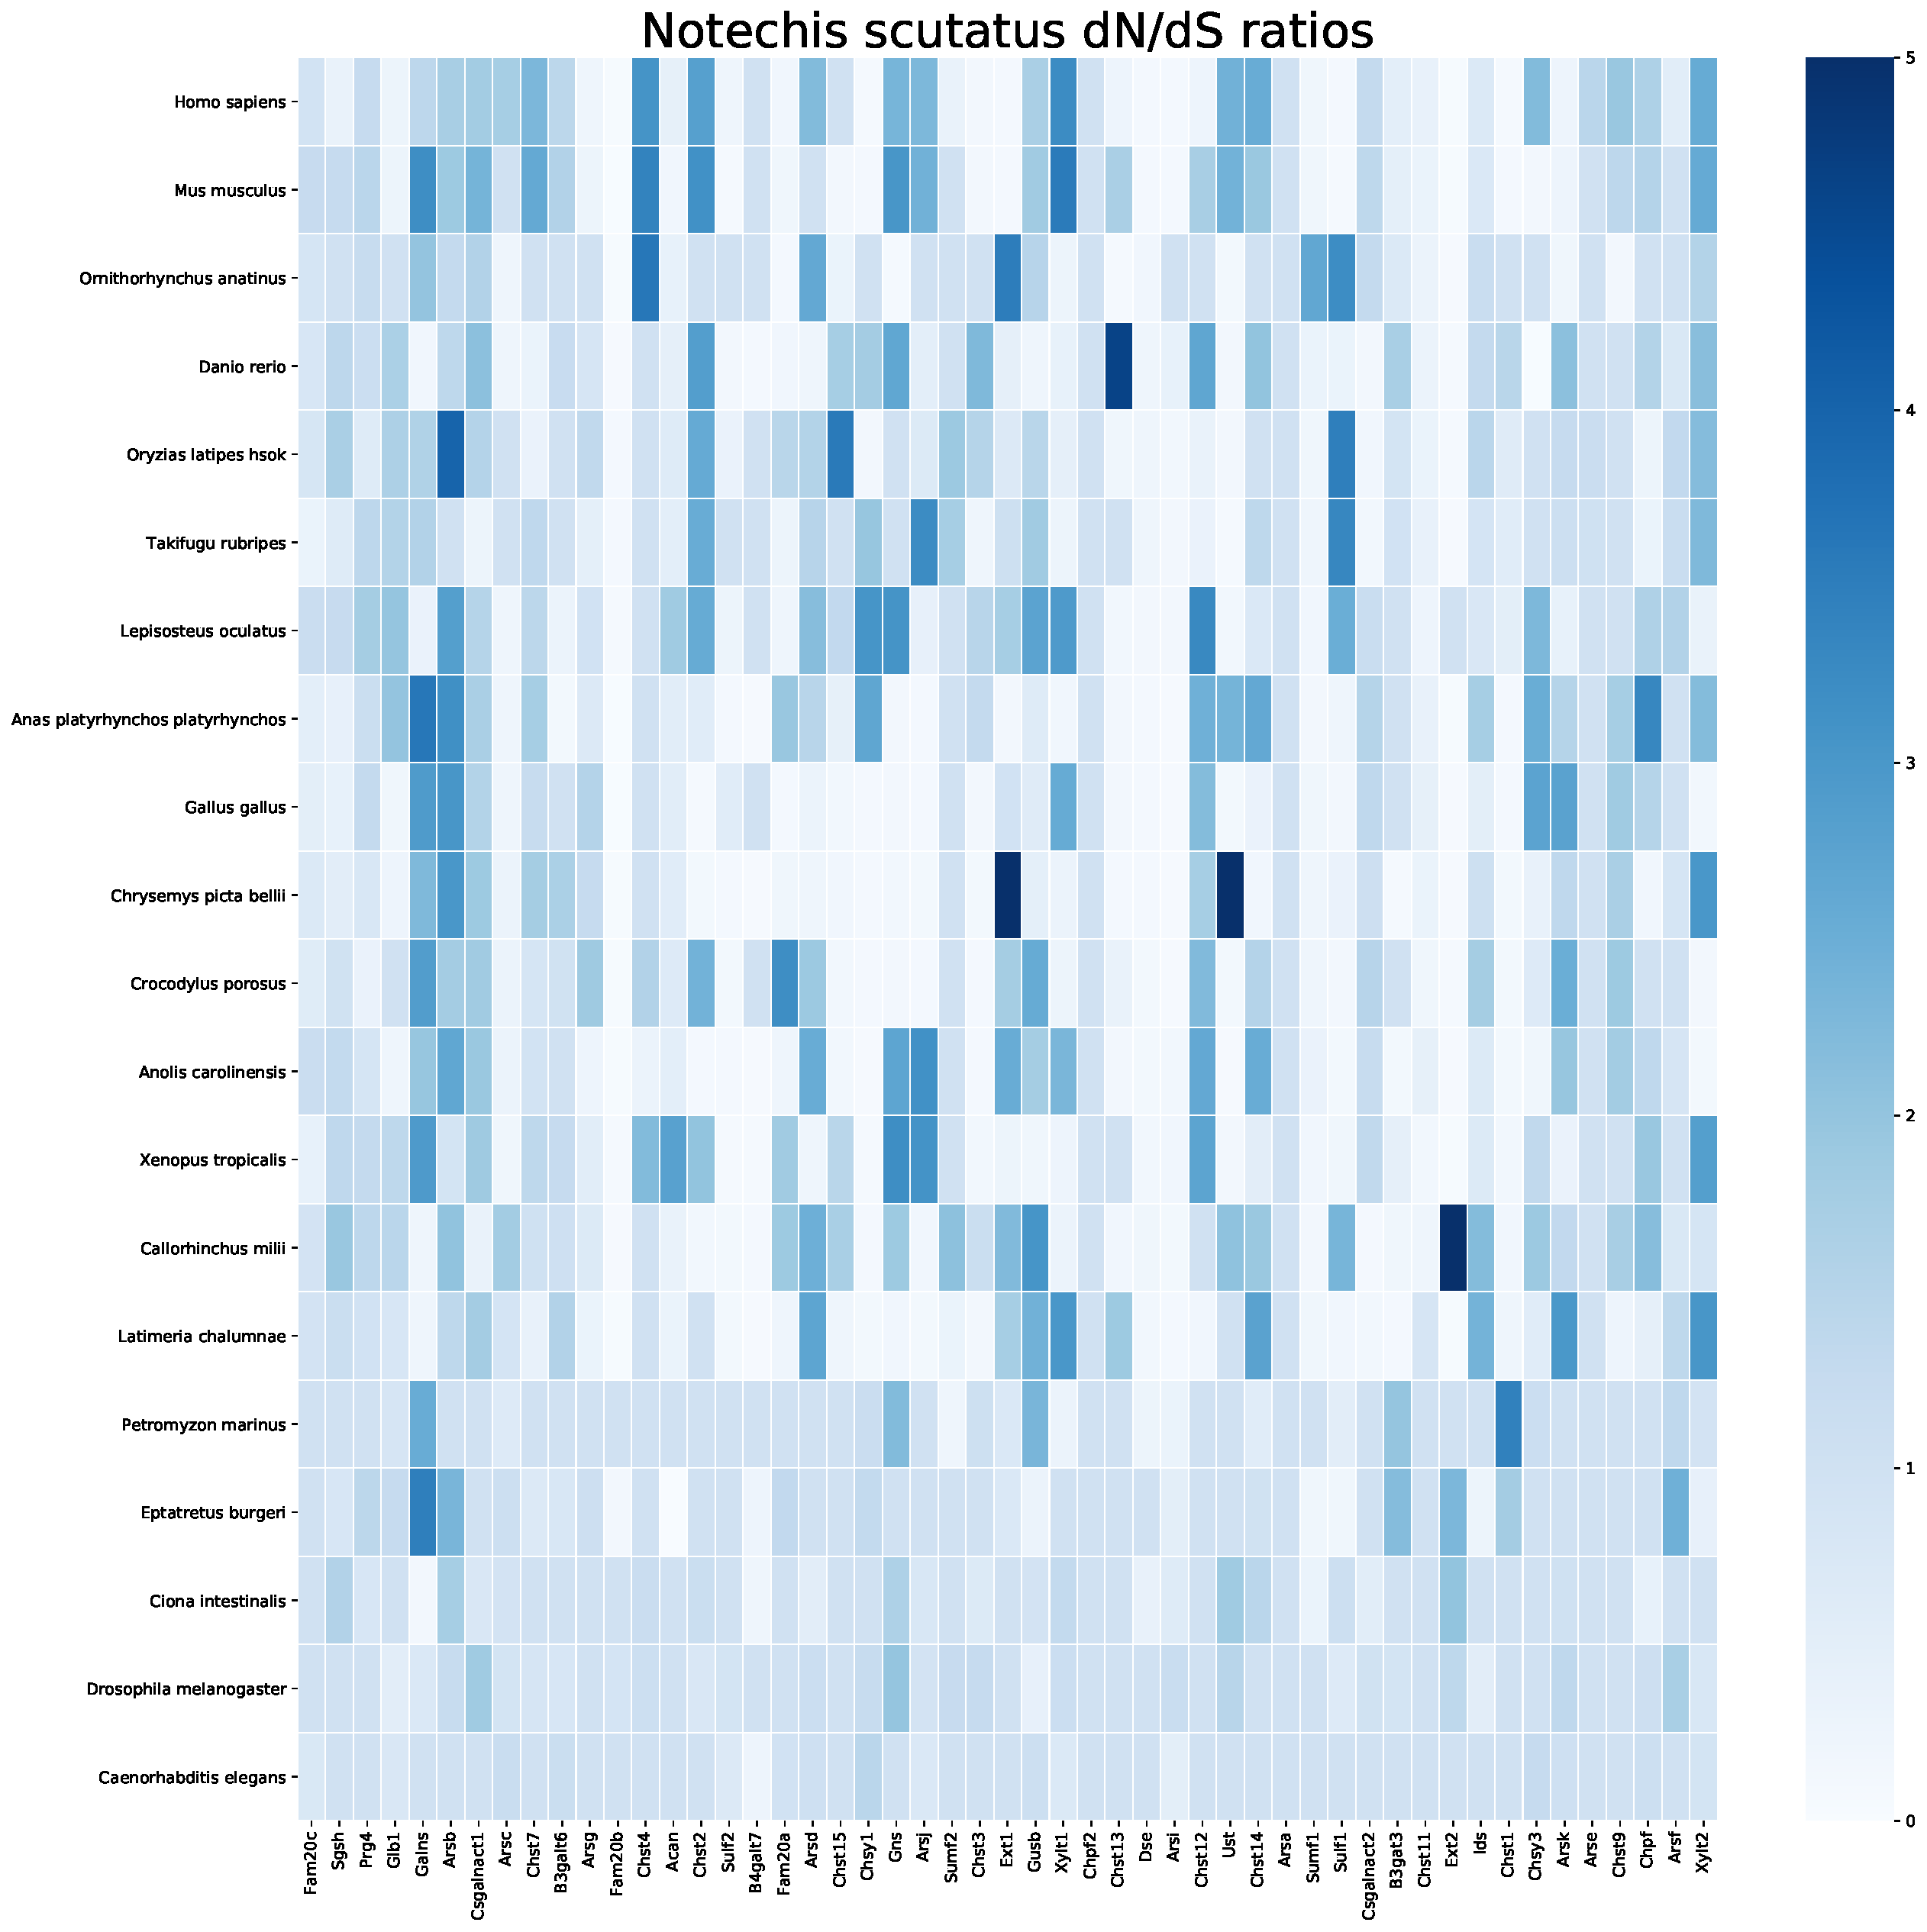
\includegraphics[height=7in,trim={0 0 0 0in},clip]{./appendix_images/dnds/notechis_scutatus.pdf}}
\caption{\textbf{dN/dS 2D grid for \textit{Notetis scutatus} computed against the other significant organisms.} The intensity values represent the dN/dS ratio - values lighter in colour are less than 1 and purifying selection while values darker in colour are greater than 1 and represent positive selection.}
\label{sup_fig_29}
\end{figure}

\begin{figure}[H]
\centering
\makebox[\textwidth][c]{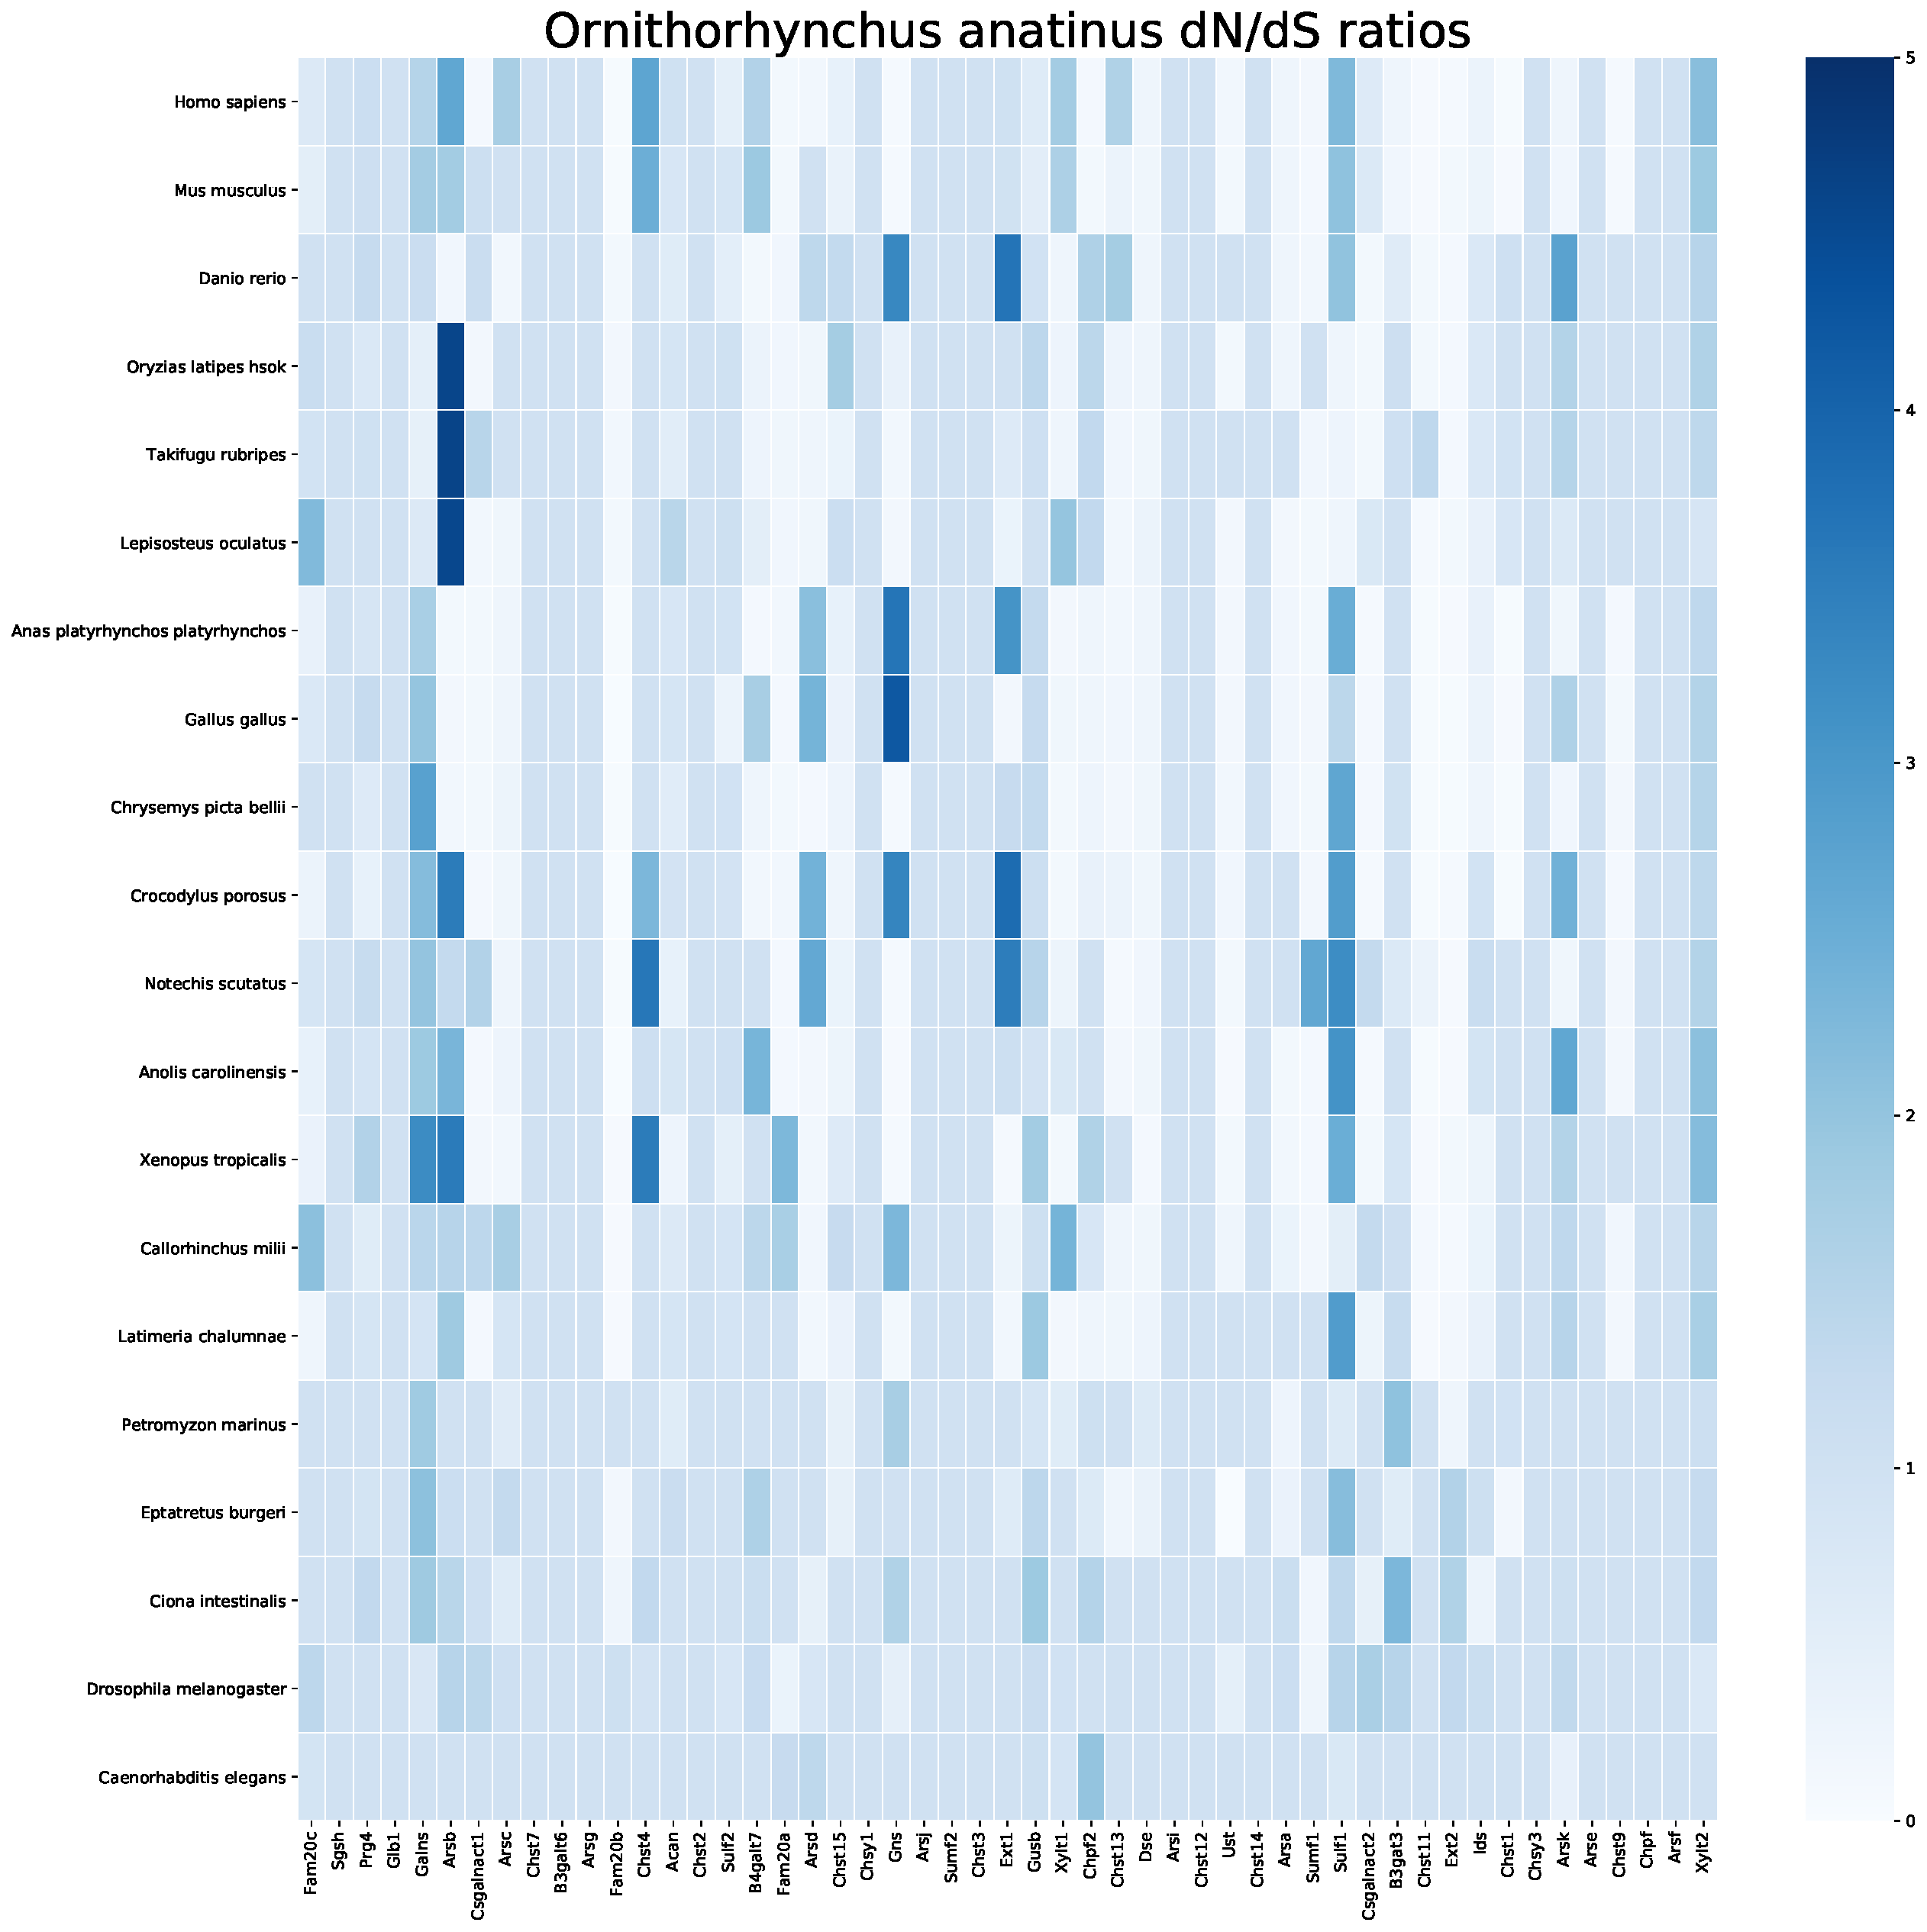
\includegraphics[height=7in,trim={0 0 0 0in},clip]{./appendix_images/dnds/ornithorhynchus_anatinus.pdf}}
\caption{\textbf{dN/dS 2D grid for \textit{Ornithorhynchus anatinus} computed against the other significant organisms.} The intensity values represent the dN/dS ratio - values lighter in colour are less than 1 and purifying selection while values darker in colour are greater than 1 and represent positive selection.}
\label{sup_fig_30}
\end{figure}

\begin{figure}[H]
\centering
\makebox[\textwidth][c]{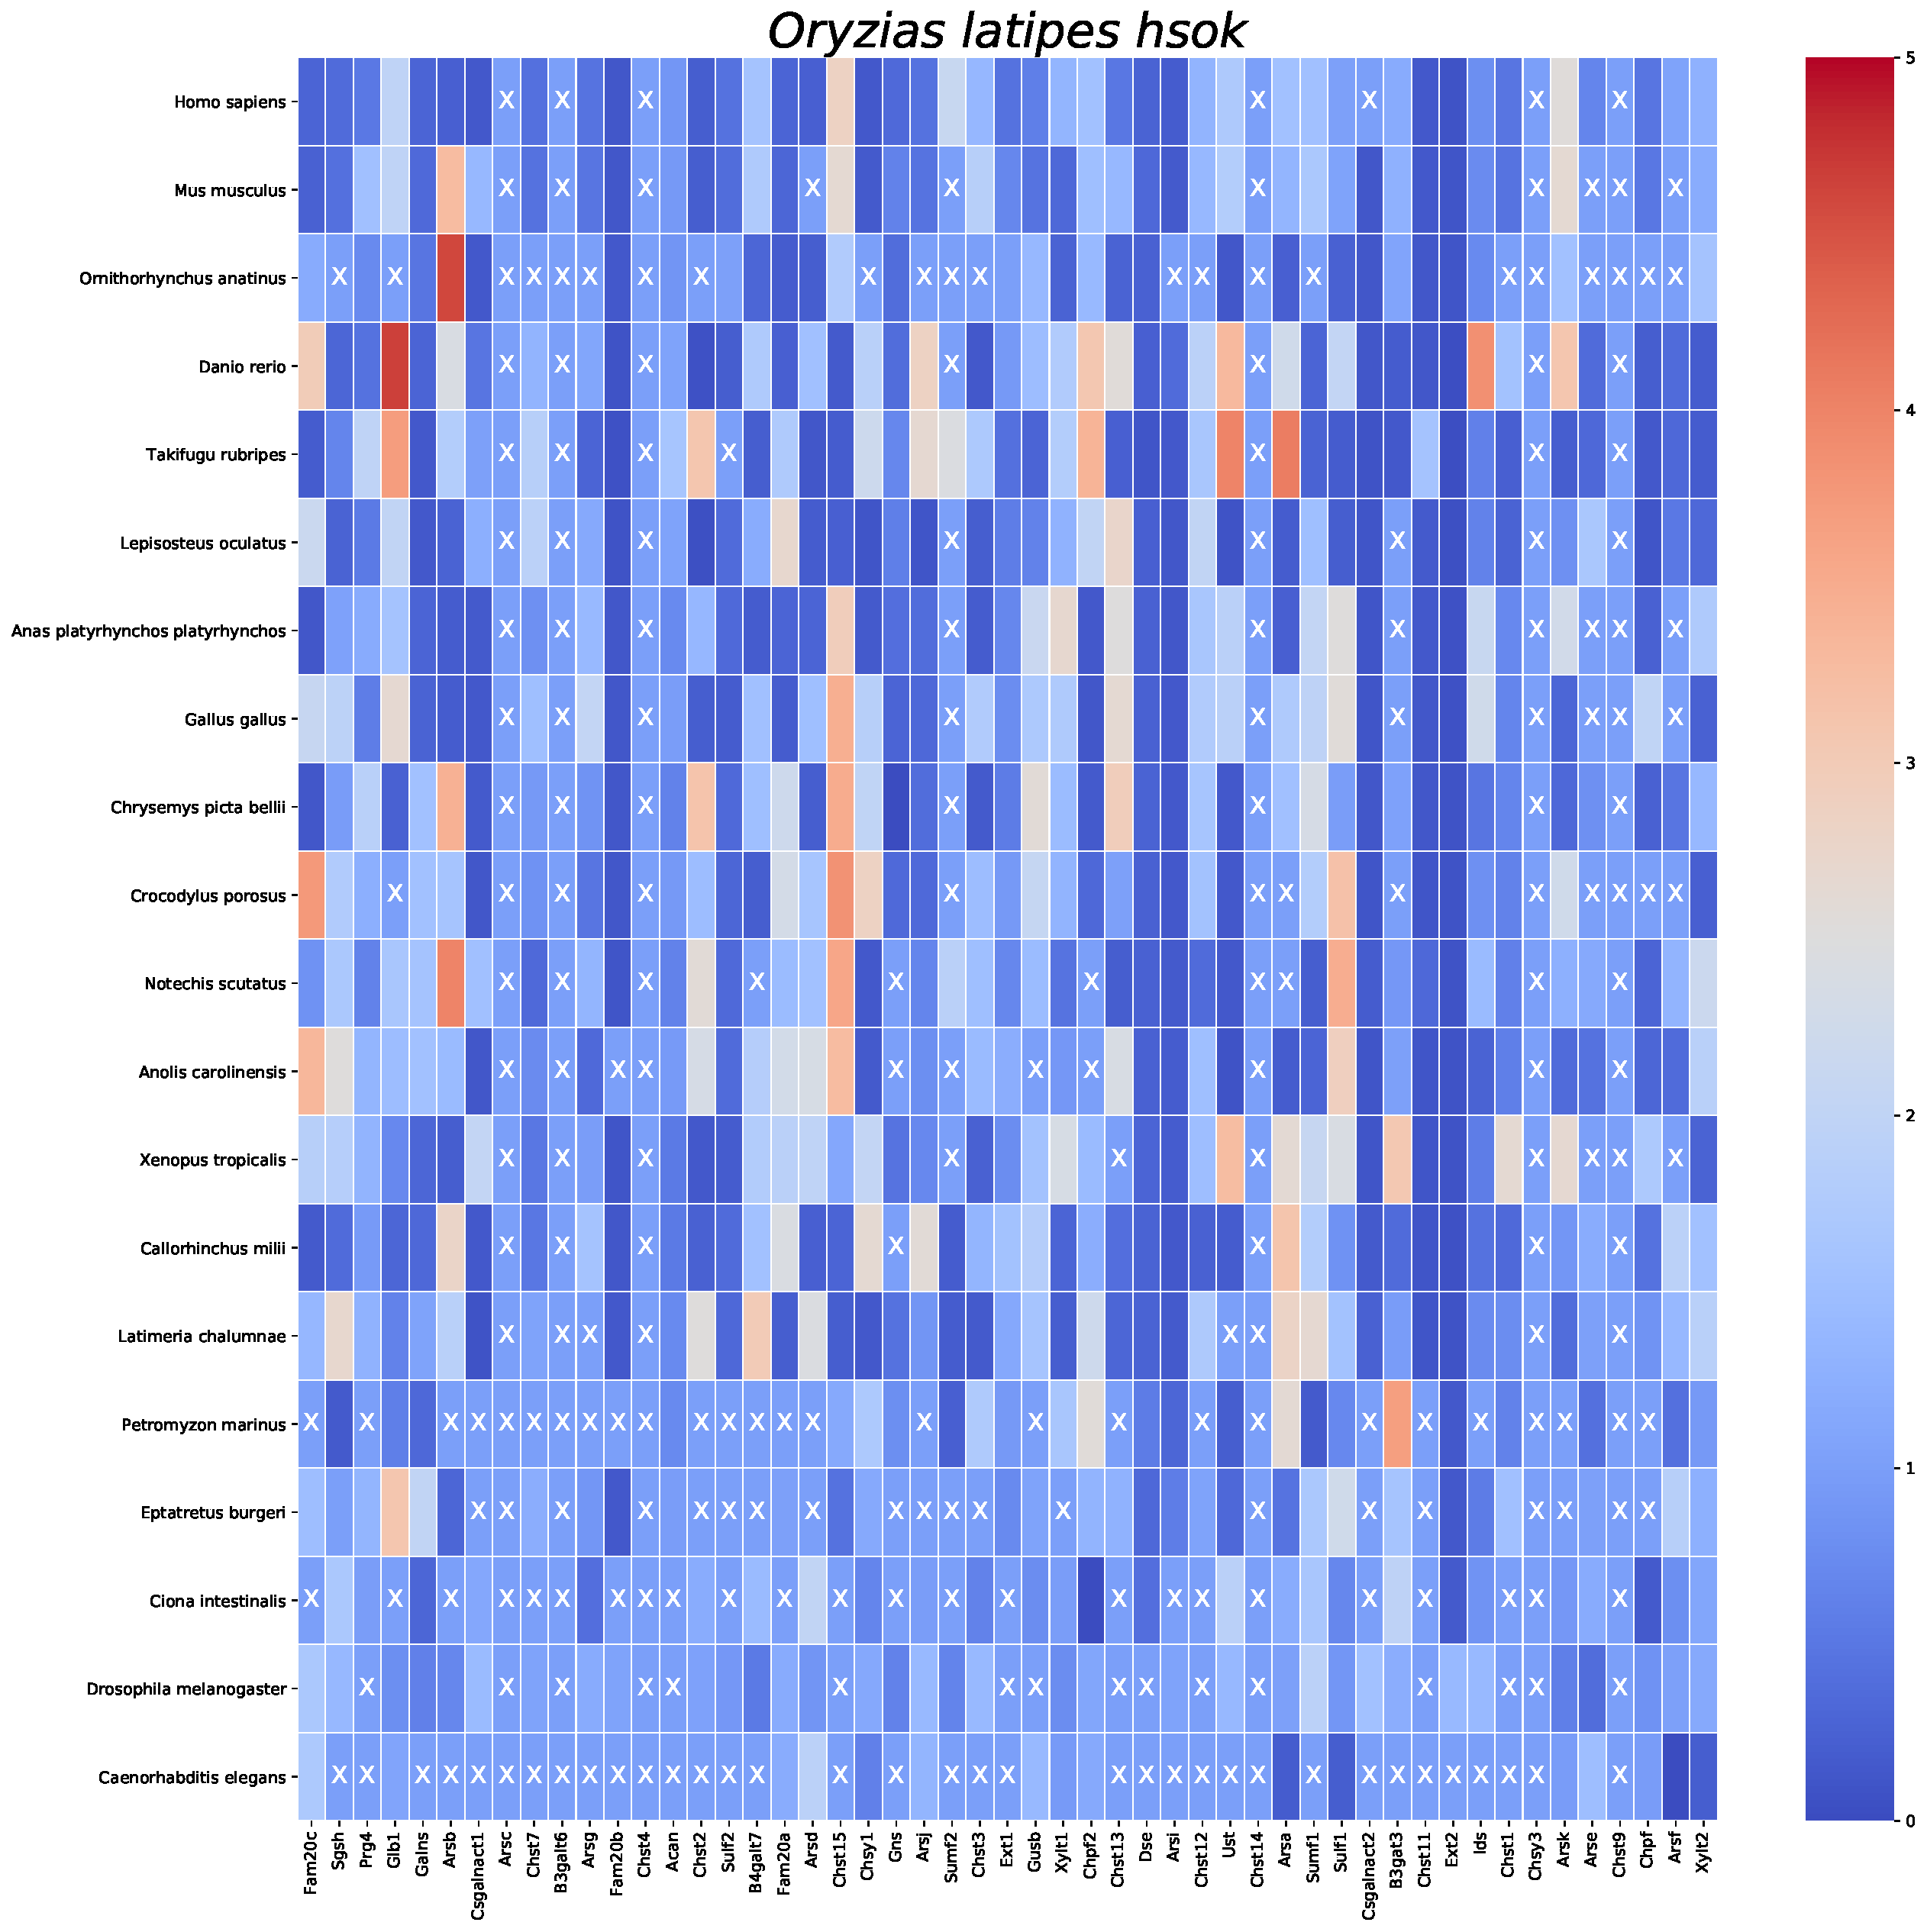
\includegraphics[height=7in,trim={0 0 0 0in},clip]{./appendix_images/dnds/oryzias_latipes_hsok.pdf}}
\caption{\textbf{dN/dS 2D grid for \textit{Oryzias latipes} computed against the other significant organisms.} The intensity values represent the dN/dS ratio - values lighter in colour are less than 1 and purifying selection while values darker in colour are greater than 1 and represent positive selection.}
\label{sup_fig_31}
\end{figure}

\begin{figure}[H]
\centering
\makebox[\textwidth][c]{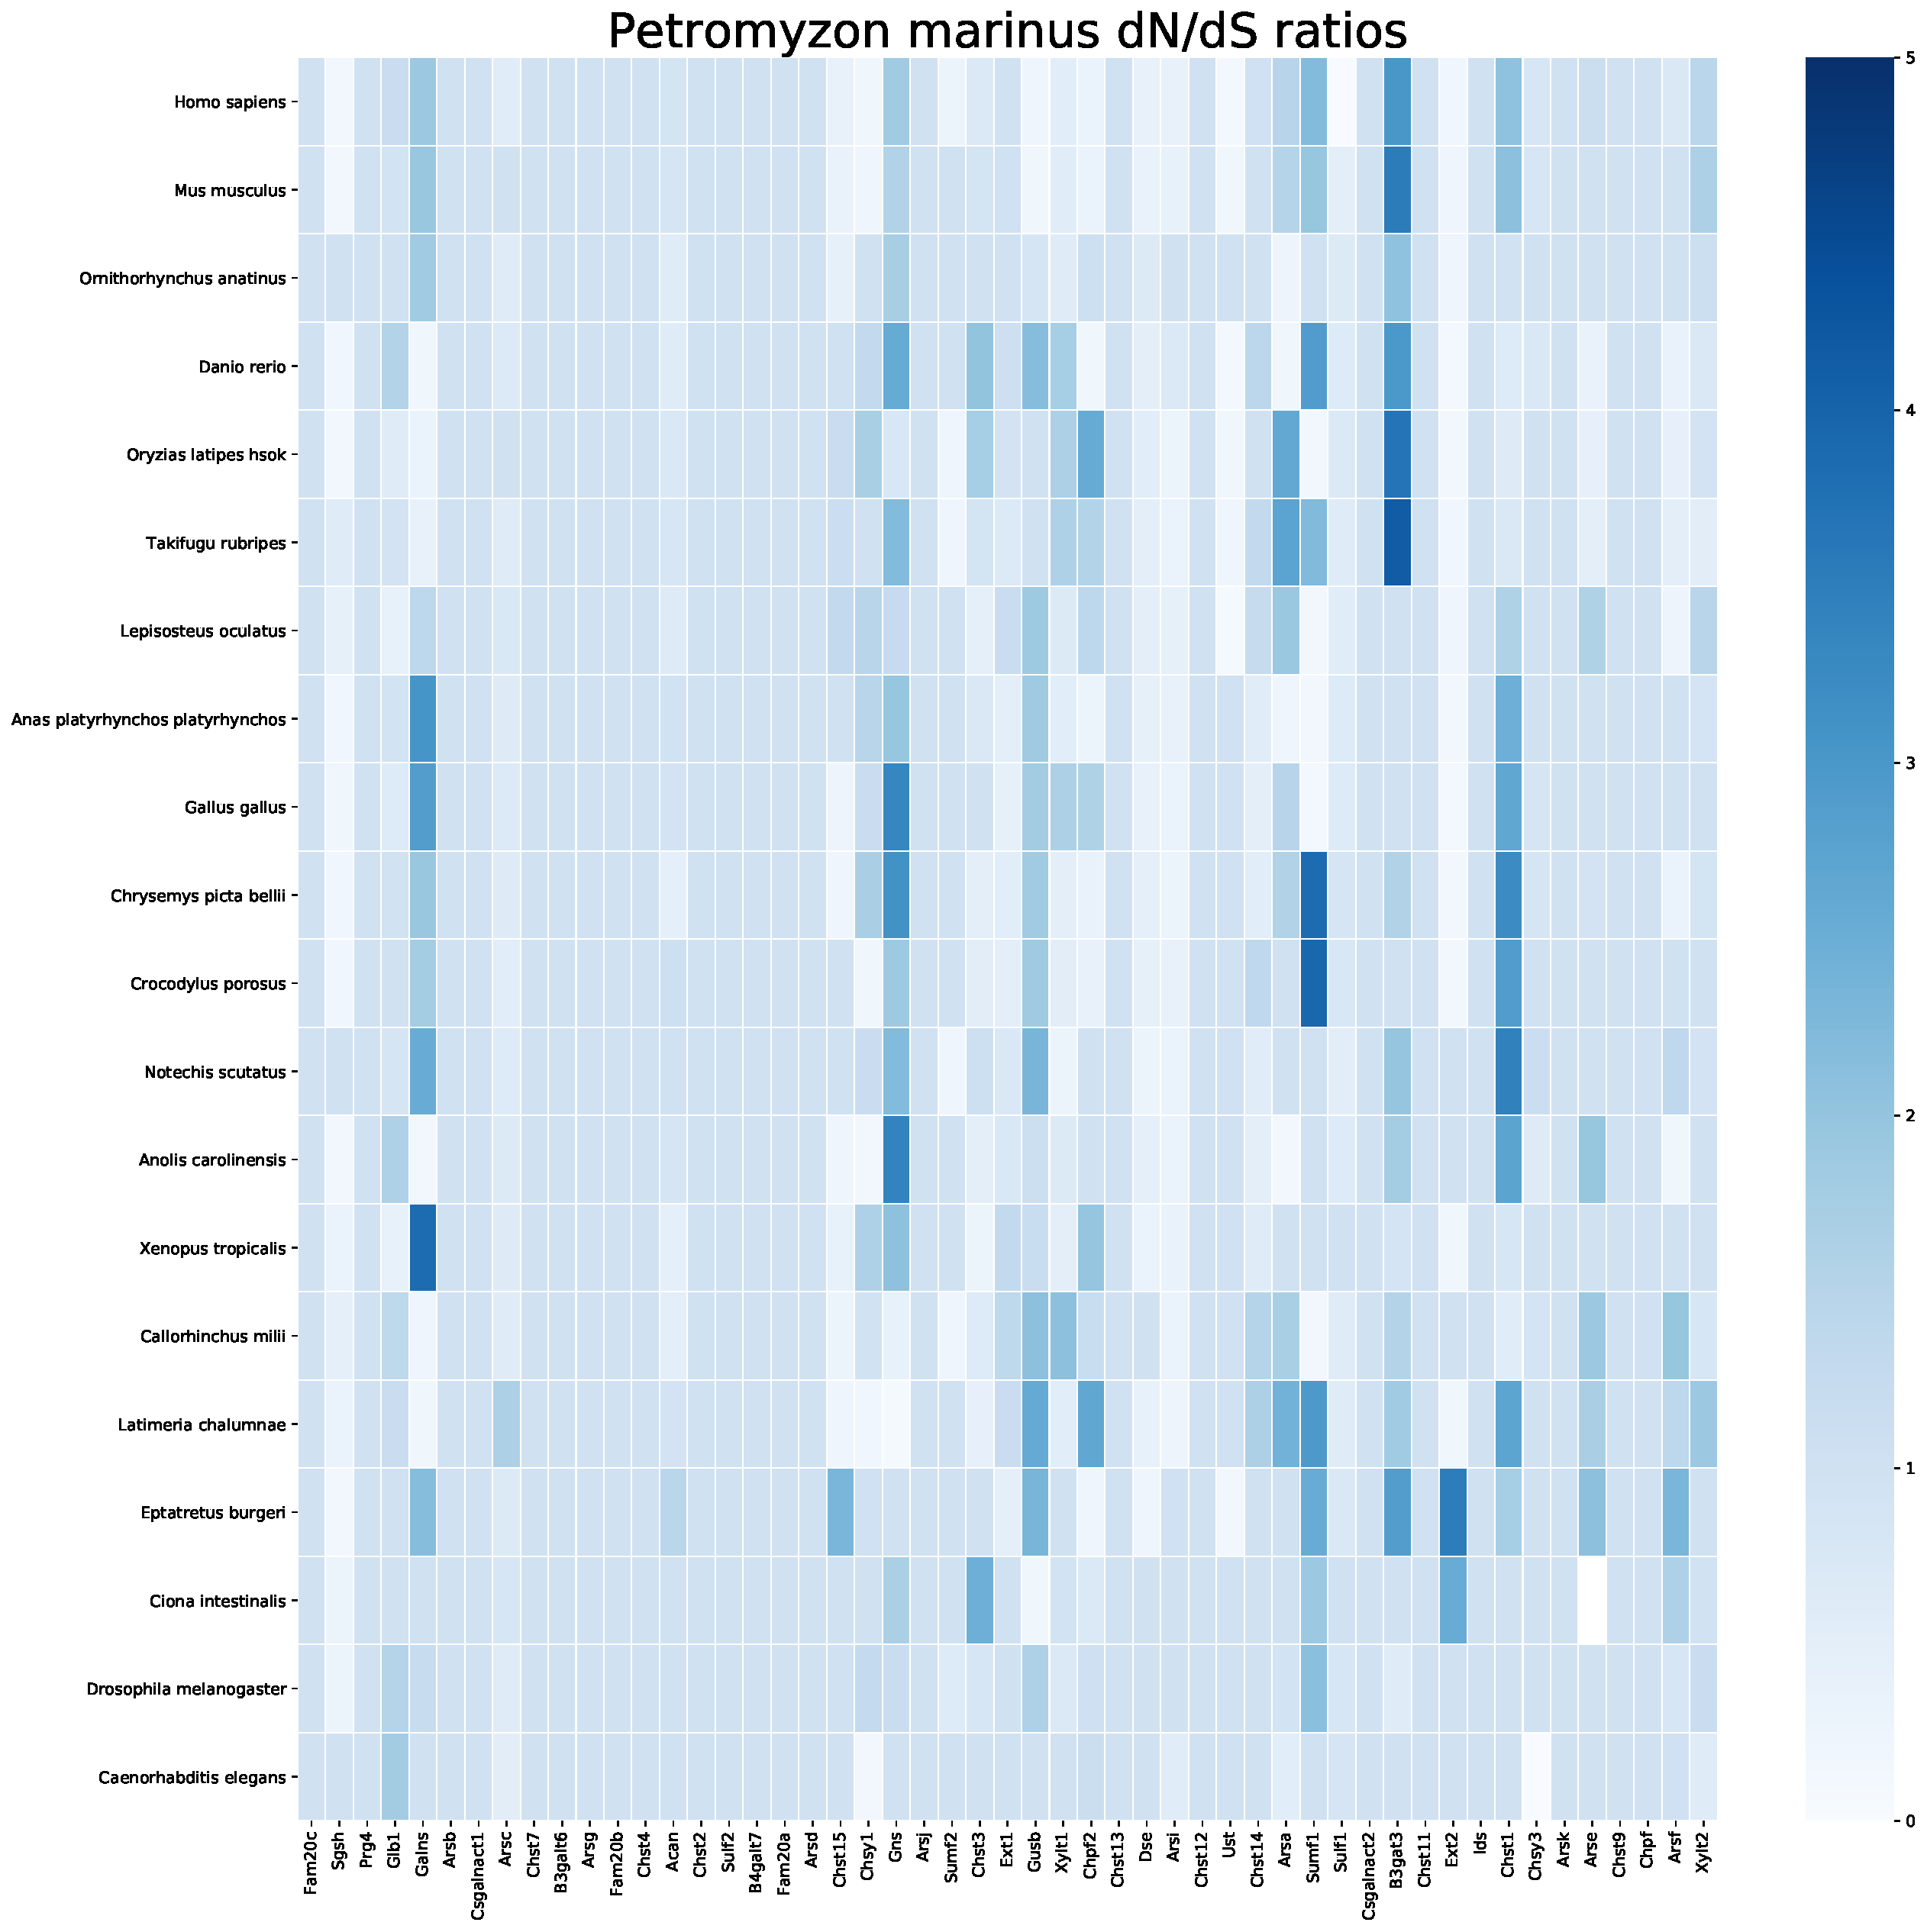
\includegraphics[height=7in,trim={0 0 0 0in},clip]{./appendix_images/dnds/petromyzon_marinus.pdf}}
\caption{\textbf{dN/dS 2D grid for \textit{Petromyzon marinus} computed against the other significant organisms.} The intensity values represent the dN/dS ratio - values lighter in colour are less than 1 and purifying selection while values darker in colour are greater than 1 and represent positive selection.}
\label{sup_fig_32}
\end{figure}

\begin{figure}[H]
\centering
\makebox[\textwidth][c]{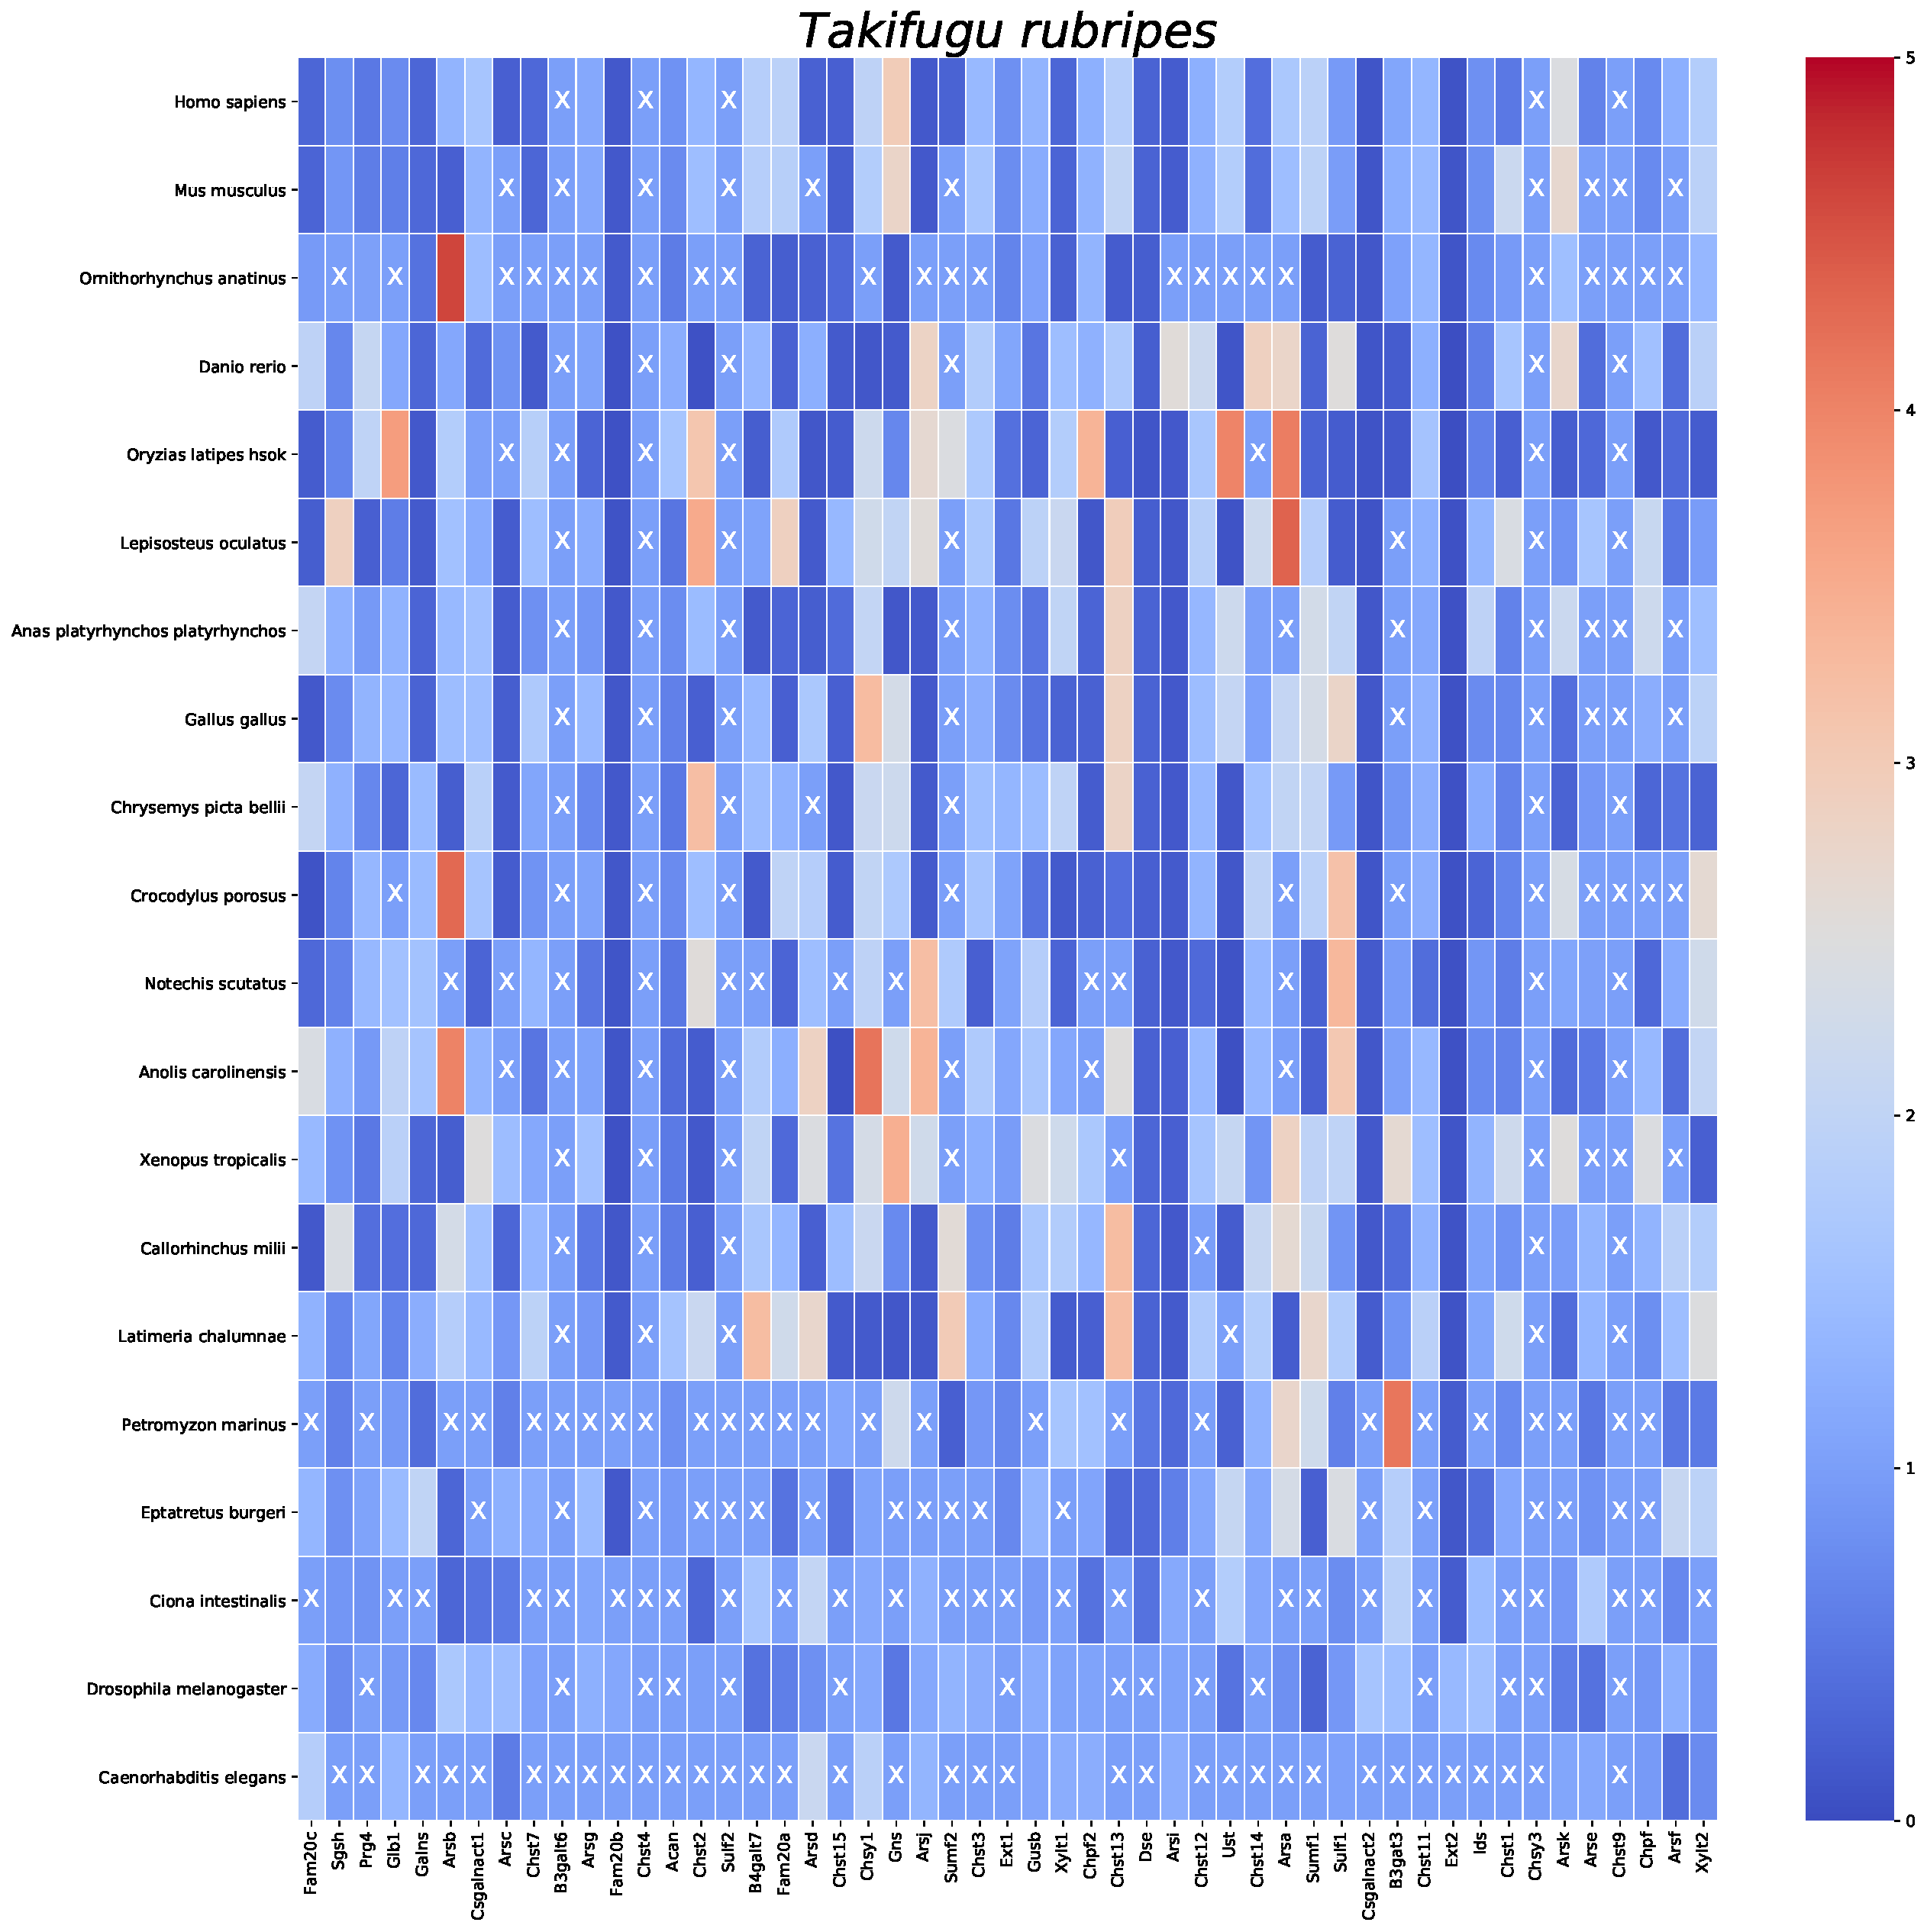
\includegraphics[height=7in,trim={0 0 0 0in},clip]{./appendix_images/dnds/takifugu_rubripes.pdf}}
\caption{\textbf{dN/dS 2D grid for \textit{Takifugu rubripes} computed against the other significant organisms.} The intensity values represent the dN/dS ratio - values lighter in colour are less than 1 and purifying selection while values darker in colour are greater than 1 and represent positive selection.}
\label{sup_fig_33}
\end{figure}

\begin{figure}[H]
\centering
\makebox[\textwidth][c]{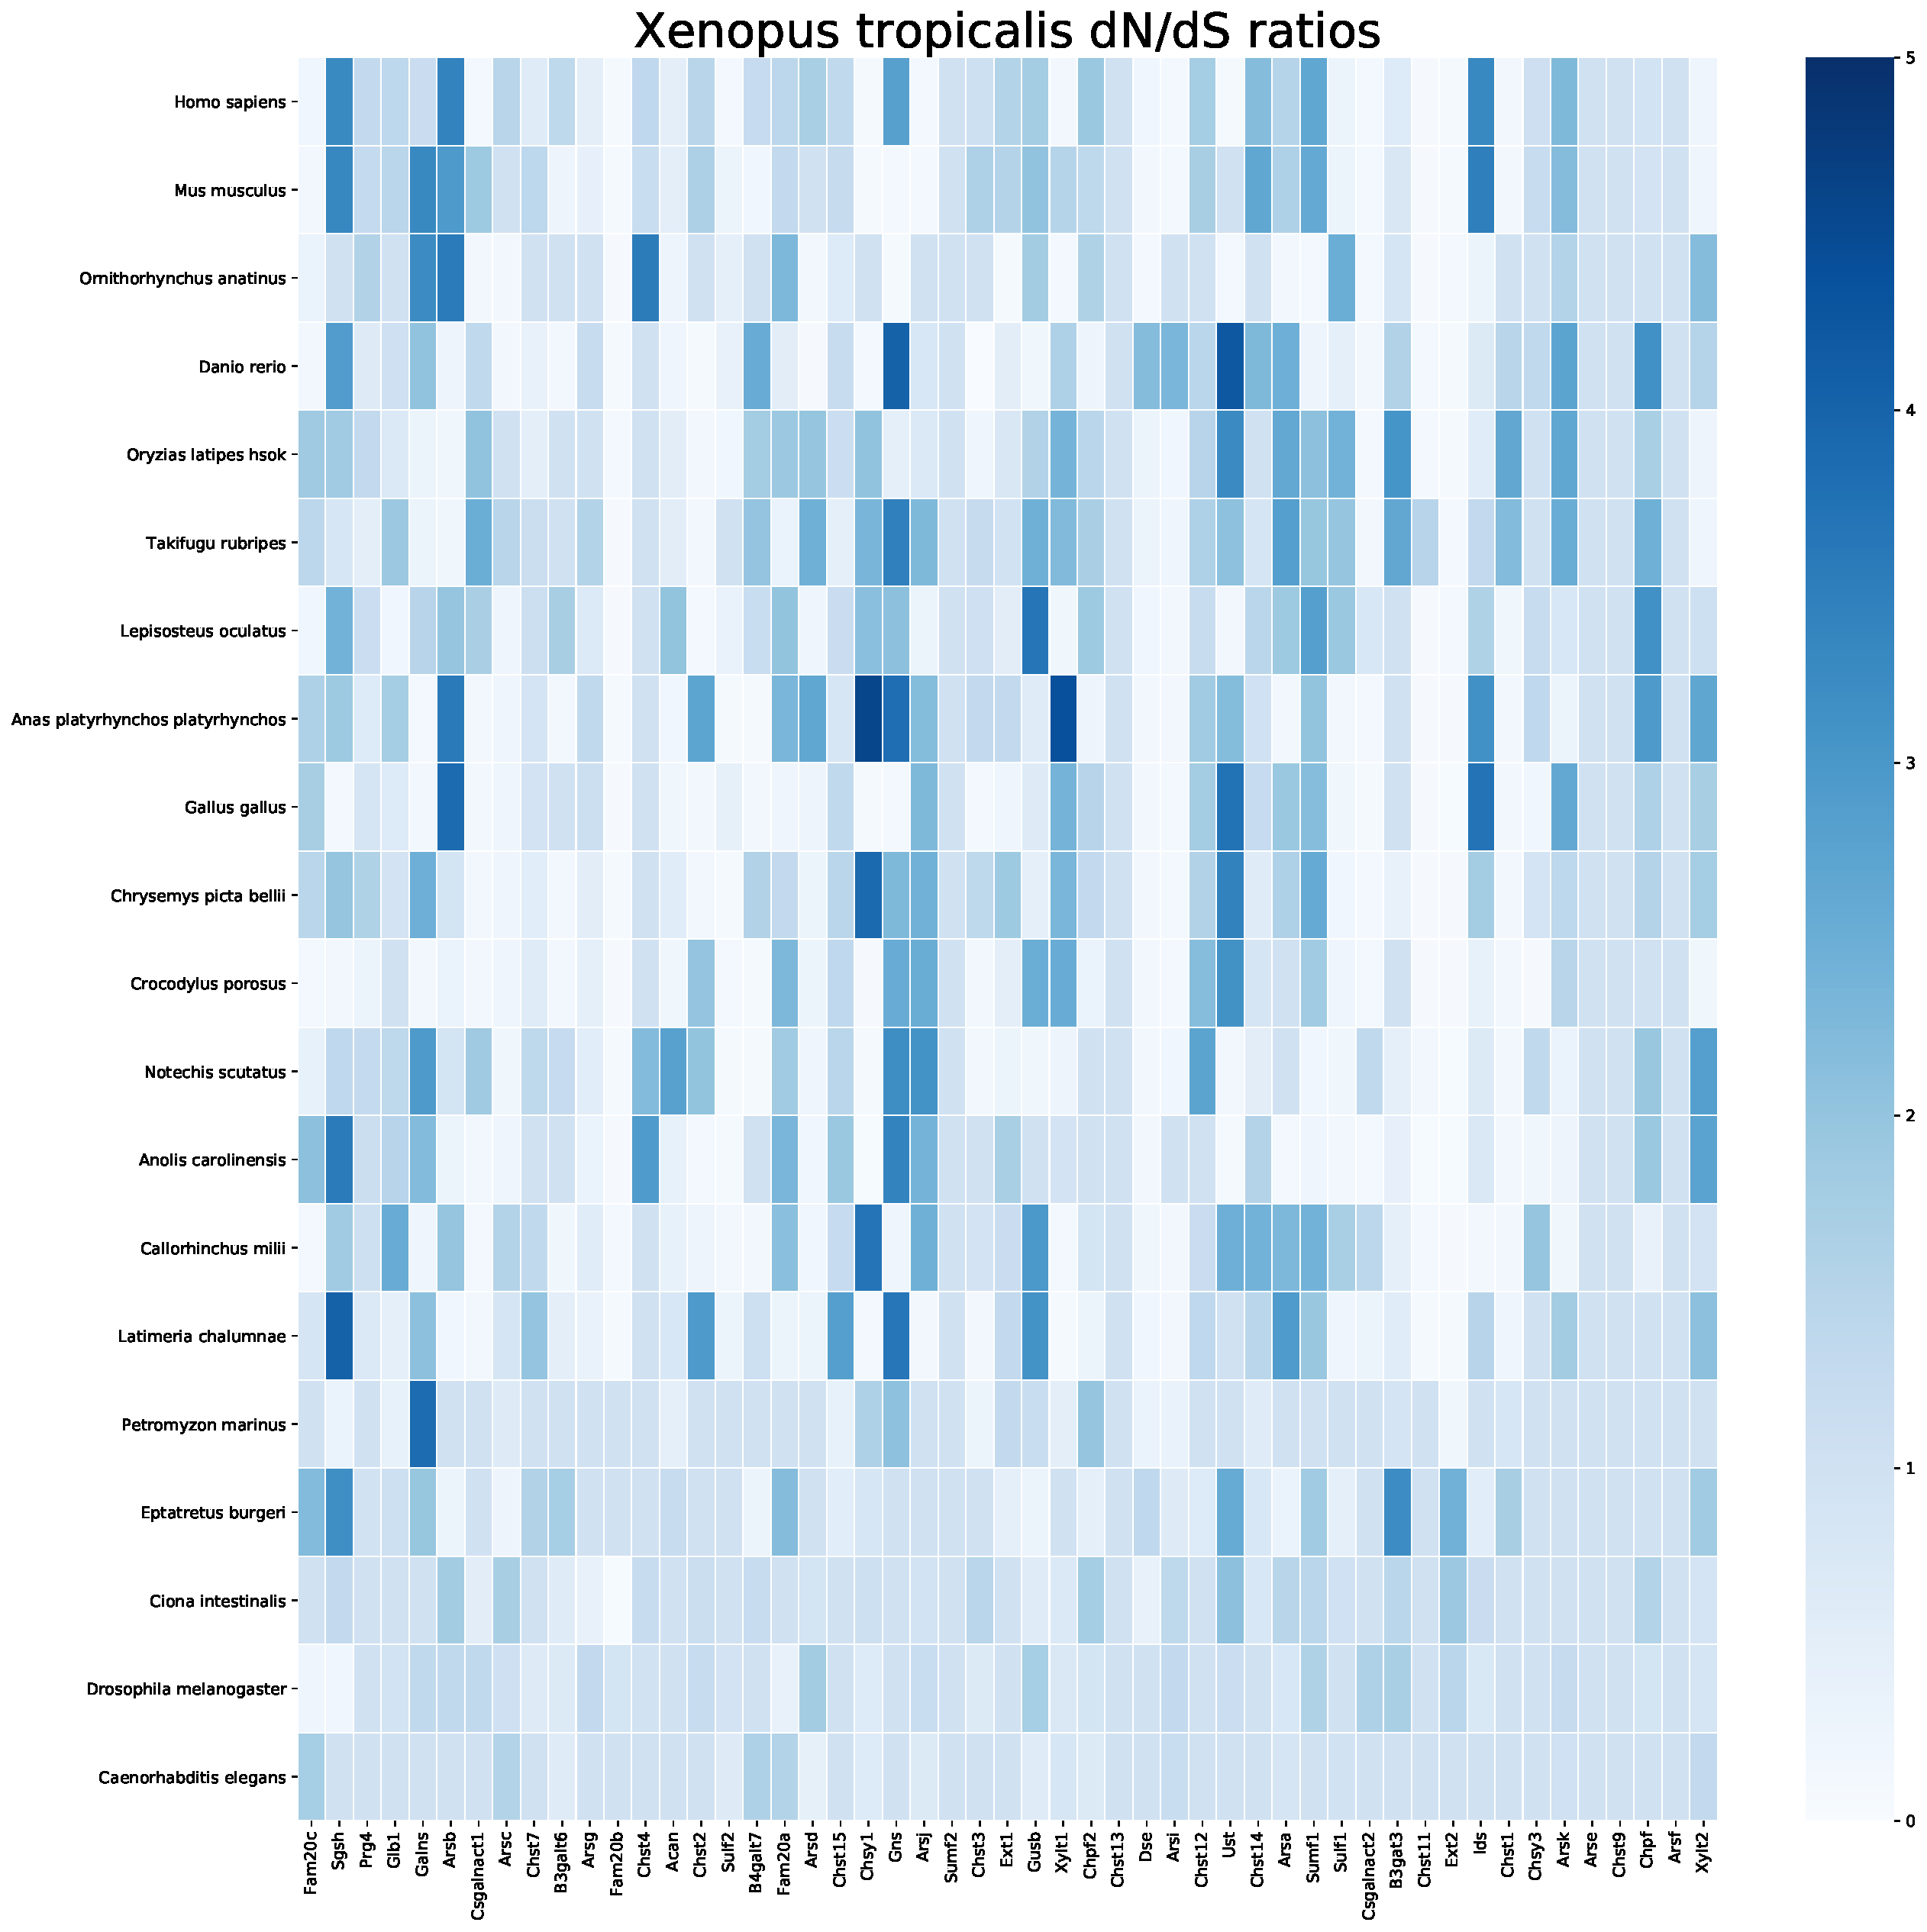
\includegraphics[height=7in,trim={0 0 0 0in},clip]{./appendix_images/dnds/xenopus_tropicalis.pdf}}
\caption{\textbf{dN/dS 2D grid for \textit{Xenopus tropicalis} computed against the other significant organisms.} The intensity values represent the dN/dS ratio - values lighter in colour are less than 1 and purifying selection while values darker in colour are greater than 1 and represent positive selection.}
\label{sup_fig_34}
\end{figure}

\end{document}